
%-----------------------------------------------------------------------------------
%	PACKAGES AND OTHER DOCUMENT CONFIGURATIONS
%-----------------------------------------------------------------------------------
\documentclass[11pt, twoside,hidelinks]{Thesis}
% The default font size and two-sided printing 
% For a one-sided printing change the flag "twoside" to "oneside" 

\graphicspath{{Figures/},{Logos/}}

% \usepackage[dvipsnames]{xcolor}
\usepackage{tikzit}
\usepackage{tikz}
\usepackage{tikz-3dplot}
\usepackage{tkz-euclide}
\usepackage{caption}
\usepackage{subcaption}
\newcommand\hmmax{0}
\newcommand\bmmax{0}
\usepackage{lipsum} % For dummy text
\usepackage{graphicx,float}% Include figure files
\usepackage{epsfig}		
\usepackage{dcolumn}% Align table columns on decimal point
\usepackage{bm}% bold math
\usepackage{amsmath}
\usepackage{etoolbox}
\usepackage[boxsize=1em,centertableaux]{ytableau}
\usepackage{pgfplots}
\pgfplotsset{compat = newest}
\usepackage{upgreek}
\usepackage{todonotes}
\usepackage{amssymb}
\usepackage{braket}
%\usepackage{mciteplus}
\usepackage[square, numbers, comma, sort&compress]{natbib} % Use the natbib reference package - read up on this to edit the reference style; if you want text (e.g. Smith et al., 2012) for the in-text references (instead of numbers), remove 'numbers' 
\usepackage{mathtools}
\usepackage{nameref}
\usepackage{notoccite}
\usepackage{enumerate}
\usepackage{dsdshorthand}
\usepackage{array, booktabs, makecell}
\usepackage{siunitx, mhchem}


\hypersetup{
  colorlinks=False,
  % citecolor=Blue,
  % linkcolor=Red,
  % urlcolor=Blue
  }
%-----------------------------------------------------------------------------------
% BIBLIOGRAPHY STYLE
%-----------------------------------------------------------------------------------

% \usepackage{natbib}
% \setcitestyle{square, numbers, comma, sort&compress}
\usepackage[square, numbers, comma, sort&compress]{natbib}
% \usepackage{chapterbib}

%%% BST STYLES
% \bibliographystyle{apsrev4-1}
% \bibliographystyle{apsrev4-1-etal}
% \bibliographystyle{unsrt}
% With emphasized titles and no comma in the last author
%TIKZ

\usetikzlibrary{arrows,calc,shapes,decorations.pathmorphing,decorations.markings}
\tikzset{
>=stealth',
help lines/.style={dashed, thick},
axis/.style={<->},
important line/.style={thick},
connection/.style={thick, dotted},
  cross/.style={
    cross out,
    draw=black, 
    minimum size=7pt, 
    inner sep=0pt,
    outer sep=0pt
  },
  branchcut/.style={
    decoration={
      snake,
      amplitude=1pt,
      segment length=6pt,
    },
    decorate,
    thick
  },
->-/.style={decoration={
  markings,
  mark=at position #1 with {\arrow{>}}},postaction={decorate}},
  twopt/.style={
    circle,
    draw,
    fill=black,
    inner sep=1pt,
    minimum size=1pt
  },
  scalar/.style={
    thick,
    dashed,
    postaction={
      decorate,
      decoration={
        markings,
        mark=at position 0.5 with {\arrow{>}}
      }
    }
  },
  spinning/.style={
    thick,
    postaction={
      decorate,
      decoration={
        markings,
        mark=at position 0.5 with {\arrow{>}}
      }
    }
  },
  scalar no arrow/.style={
    thick,
    dashed,
  },
  spinning no arrow/.style={
    thick,
  },
  finite/.style={
    decoration={
      snake,
      amplitude=1pt,
      segment length=6pt,
    },
    decorate,
    thick
  },
  axis/.style={
    thick,
    postaction={
      decorate,
      decoration={
        markings,
        mark=at position 1 with {\arrow{>}}
      }
    }
  },
}

\tikzset{snake it/.style={decorate, decoration=snake , samples = 100}}
%-----------------------------------------------------------------------------------
% FONTS & SPECIAL CHARACTERS
%-----------------------------------------------------------------------------------

\usepackage{mathpazo}% default 
% \usepackage[notextcomp]{stix}% Times font like package with math support 
% \usepackage{fourier}
% \usepackage{palatino}% ( mathpazo on text + Computer Modern on math )
%\usepackage{newpxtext,newpxmath}


%-----------------------------------------------------------------------------------
%	DOCUMENT VARIABLES
%-----------------------------------------------------------------------------------

\thesistitle[Header title]{Topics in Conformal Regge theory} % Thesis title
\author[mailto:salgarkaraaditya@fc.up.pt]{Aaditya \textsc{Salgarkar}} % Your name
% \address{} % Your address
% \subject{} % Your subject area
\keywords{ conformal field theory, AdS-CFT correspondence, holography , Regge theory , high energy scattering } % Keywords for your thesis 
\supervisor[mailto:]{Prof. Miguel \textsc{Costa}} % Your supervisor's name
%\cosupervisor[mailto:name@host.com]{John \textsc{Doe}} % Your co-supervisor's name
% To hide the co-supervisor field, just comment out \cosupervisor[<url>]{<name>}  
\degree{Doctor of Philosophy}{Doctoral} % Your degree name
\university[http://www.univesityurl.com]{University of Porto} % Your university's name
\department[http://www.departmenturl.com]{Departament of Physics and Astronomy} % Your department's name 
% To hide the Department field, just comment out \department[<url>]{<name>}         
\group[http://www.groupurl.com]{Centro de Física do Porto} % Your research group's name
% To hide the Group field, just comment out \group[<url>]{<name>}    
\faculty[http://www.facultyurl.com]{Faculty of Sciences} % Your faculty's name
% To hide the Faculty field, just comment out \faculty[<url>]{<name>}  
\logos[15mm]{{Logos/up2},{Logos/fc}}
% To hide the logos, just comment out \logos{<relative location>}  


%-----------------------------------------------------------------------------------
%	NOTATION VARIABLES
%-----------------------------------------------------------------------------------

\newcommand{\dd}{\mathrm{d}}
\newcommand{\fractd}[2][]{\frac{\dd #1}{\dd #2}}
\newcommand{\fracpd}[2][]{\frac{\partial #1}{\partial #2}}
\newcommand{\uu}[3][]{\,{}_{#1} #2_{#3}}
\renewcommand{\Re}{\mathrm{Re}}
\renewcommand{\Im}{\mathrm{Im}}
\def\bb#1{\mbox{\footnotesize $(#1)$}}
\def\bkR{{\rm I\kern-.17em R}}
\def\half{{\textstyle{1\over 2}}}
\newcommand*{\defeq}{\mathrel{\vcenter{\baselineskip0.5ex \lineskiplimit0pt
           \hbox{\scriptsize.}\hbox{\scriptsize.}}}%
           =}
\newcommand{\bea}{\begin{equation}\begin{aligned}}
\newcommand{\eea}[1]{\label{#1}\end{aligned}\end{equation}}
\DeclareMathOperator \Disc {Disc}




\newcommand{\beq}{\begin{equation}}
\newcommand{\eeq}{\end{equation}}
\newcommand   \xb  {\bar{x}}
\newcommand   \zb  {\bar{z}}
\newcommand   \wb  {\bar{w}}
\newcommand   \pb  {{\bar{p}}}
\newcommand   \kb  {\bar{k}}
\newcommand   \vb  {\bar{v}}
\newcommand   \Deb  {\bar{\De}}
\newcommand   \ellb  {\bar{\ell}}
\newcommand   \nb  {\bar{n}}
\newcommand{\dDisc}{\text{dDisc}}
\def\Cut{{\mathbf{Cut}}}
\def\hCut{\widehat\Cut}
\def\1{{\rm 1-loop}}

\def\TODO#1{{\bf[TODO: #1]}}
\def\THnote#1{{\bf[TH: #1]}}


\newcommand{\diagramEnvelope}[1]{#1}










\newcommand{\non}{\nonumber}
\newcommand{\ubar}[1]{\underline{#1}}
\newcommand   \bnu  {\boldsymbol{\nu}}
\newcommand   \bmu  {\boldsymbol{\mu}}
\newcommand   \brho  {\boldsymbol{\rho}}

\newcommand   \balpha  {\boldsymbol{\alpha}}
\newcommand   \bbeta  {\boldsymbol{\beta}}
\newcommand   \bgamma  {\boldsymbol{\gamma}}
\newcommand   \bdelta  {\boldsymbol{\delta}}

%-----------------------------------------------------------------------------------
%	DOCUMENT
%-----------------------------------------------------------------------------------

\begin{document}

\frontmatter % Use roman page numbering style for the pre-content pages

% \maketitle % Make title page
%region

%-----------------------------------------------------------------------------------
%	QUOTATION PAGE
%-----------------------------------------------------------------------------------
% \vspace{1cm}
% \quotepage{Richard Feynman}{%
  % It doesn’t make any difference how beautiful your guess is, it doesn’t make any difference how smart you are, who made the guess, or what his name is. If it disagrees with experiment, it’s wrong. That’s all there is to it.}
% \vspace{1cm}
% \vfill
% \cleardoublepage
%-----------------------------------------------------------------------------------
%	Sworn statement
%-----------------------------------------------------------------------------------

\begin{frontchapter}{Sworn statement} \label{sworn_statement}

  I, Aaditya Salgarkar, enrolled in the Doctor’s Degree of Physics at the Faculty of Sciences of the
University of Porto hereby declare, in accordance with the provisions of paragraph a) of
Article 14 of the Code of Ethical Conduct of the University of Porto, that the content of
this thesis reflects perspectives, research work and my own interpretations at the time
of its submission.
By submitting this thesis, I also declare that it contains the results of my own research
work and contributions that have not been previously submitted to this or any other
institution.
I further declare that all references to other authors fully comply with the rules of
attribution and are referenced in the text by citation and identified in the bibliographic
references section. This thesis does not include any content whose reproduction is
protected by copyright laws.
I am aware that the practice of plagiarism and self-plagiarism constitute a form of
academic offense.
\end{frontchapter}
\cleardoublepage


%-----------------------------------------------------------------------------------
%	ACKNOWLEDGEMENTS
%-----------------------------------------------------------------------------------

\begin{acknowledgements}

  First, I would like to thank my advisor, Professor Miguel Costa, for giving me the opportunity do work in the group.
  I would specially like to thank for making part of the Simons Collaboration on nonperturbative bootstrap which helped me understand the important ideas in the field by joining stimulating discussions in the conferences.
  His high standards for the research were instrumental in my development as a researcher and the work in this thesis.
  I thoroughly enjoyed working with him and I am grateful for his guidance, support and specially his patience.
  
  I would also like to thank the Simons foundation (grant ID 488637) for providing me the funding throughout my PhD as well as several conferences.
  
  I was fortunate to have several amazing collaborators during my PhD.
  I am grateful to them for the exchange of ideas and discussions about finished projects, as well as the several ideas for future projects.
  Therefore, I would like to thank António, Balt VR, Vasco, João P, João VB, Sourav, Miguel.
  
  I would like to thank all the friends I have made during my time in Porto inside and outside the university.
  
  Finally, I would like to thank my parents for all the support they have provided me throughout my life and specially the patience during my PhD, without which this work would not have been possible.
  This thesis is dedicated to them.
\end{acknowledgements}


%-----------------------------------------------------------------------------------
%	DEDICATORY
%-----------------------------------------------------------------------------------

\begin{dedicatory}
  To 
  Aai, Baba
\end{dedicatory}

\addvspacetoc{3mm} % Add a gap in the Contents, for aesthetics

%-----------------------------------------------------------------------------------
%	ABSTRACT PAGE
%-----------------------------------------------------------------------------------

\begin{abstract}
  %\lipsum[10-20]
  In this thesis, we discuss two aspects of conformal field theory, more specifically, the conformal Regge theory.
  Conformal field theories are a special class of quantum field theories with enhanced symmetry under the group of conformal transformations.
  Regge limit is a special kinematical limit of observables in conformal field theories analogous to the high energy limit of the flat space scattering amplitude.
  First, we discuss the generalization of Optical theorem from flat space to $ AdS $ space, in the Regge limit.
  We discuss its relation to the flat space optical theorem in the appropriate limit.
  Second, we discuss the generalization of conformal Regge theory to higher point correlation functions.
  In particular, we propose the kinematics in the position space for the higher point correlation functions and show that they are equivalent to a natural generalization from the multi Regge limit of the flat space scattering amplitude.
\end{abstract}

%-----------------------------------------------------------------------------------
%	ABSTRACT PAGE (PORTUGUESE)
%-----------------------------------------------------------------------------------

\begin{abstract}[title={Resumo},thesistitle={Tópicos em teoria de Regge conforme},degree={Doutor de Ciência},nameconnector={por}]
  
  Nesta dissertação, discutimos dois aspetos da teoria de campos conformes, particularmente, a teoria de Regge conforme.
  As teorias de campos conformes são uma classe especial de teorias de campos quânticos com simetria aprimorada sob o grupo de transformações conformes.
  O limite de Regge é um limite cinemático especial de observáveis em teorias de campos conformes, análogo ao limite de alta energia da `Scattering amplitude' de espaço plano.
  Em primero lugar, discutimos a generalização do teorema ótico de espaço plano para o espaço $AdS$, no limite de Regge.
  Adicionalmente, discutimos a sua relação com o teorema ótico de espaço plano no limite apropriado.
  Em segundo lugar, discutimos a generalização da teoria conforme de Regge para funções de correlação com mais de quatro pontos.
  Em particular, propomos a cinemática no espaço de posição para funções de correlação de mais de quatro pontos e mostramos que são equivalentes a uma generalização natural do limite multi Regge da `Scattering amplitude' de espaço plano. 
  
\end{abstract}


%-----------------------------------------------------------------------------------
%	LIST OF CONTENTS/FIGURES/TABLES
%-----------------------------------------------------------------------------------

\addvspacetoc{3mm} % Add a gap in the Contents, for aesthetics

\tableofcontents % Write out the Table of Contents

\listoffigures % Write out the List of Figures

\listoftables % Write out the List of Tables

%\addvspacetoc{3mm} % Add a gap in the Contents, for aesthetics


%-----------------------------------------------------------------------------------
%	PHYSICAL CONSTANTS/OTHER DEFINITIONS
%-----------------------------------------------------------------------------------

% \begin{listofcontants}
% 	\const{My little ponny test of magical rainbow}{$m_n/m_p$}{$2.997\ 924\ 58\times10^{8}\ \text{m\,s}^{-1}$}
% 	\const{Vaccuum permeability test of magical rainbow for a specific case of condensed matter physics}{$\epsilon_0$}{$2.997\ 924\ 58\times10^{8}\ \text{m\,s}^{-1}$}
% 	\const{Speed of Light test of magical rainbow}{$c$}{$2.997\ 924\ 58\times10^{8}\ \text{m\,s}^{-1}$}
% \end{listofcontants}


%-----------------------------------------------------------------------------------
%	SYMBOLS
%-----------------------------------------------------------------------------------

% \begin{listofsymbols}
% 	\symb{$F_{\mu\nu}$}{Maxwell tensor}{F}
% 	\symb{$a$}{distance}{m}
% 	\\
% 	\symb{$\omega$}{angular frequency}{rads$^{-1}$}
% \end{listofsymbols}


%-----------------------------------------------------------------------------------
%	NOTATION
%-----------------------------------------------------------------------------------

% \begin{frontchapter}{Notation and Conventions} \label{notation}
%   \begin{align}
%     z,\bar{z}         & \quad \text{cross ratios for the four point functions in CFT }                               \\ 
%     s, t              & \quad \text{Mandelstam invariants for the two to two scattering in QFT}                      \\ 
%     \rho , \bar{\rho} & \quad \text{Radial coordinates}                                                              \\ 
%     \dDisc            & \quad \text{double discontinuity}                                                            \\ 
%     G_{\Delta,J}      & \quad \text{Conformal block of operator with the representation $ \left( \Delta,J \right) $} \\
%     g_{\Delta,J}      & \quad \text{pure Conformal block, a single solution to Casimir equation}
%   \end{align}
  
  
% \end{frontchapter}

%-----------------------------------------------------------------------------------
%	NOTATION
%-----------------------------------------------------------------------------------

\begin{frontchapter}{Publications} \label{Publications}
During the period of his PhD, the author contributed to the publication of the three works
below.
This thesis focuses on the first and the last publication of this list
\begin{enumerate}
  \item A. Antunes, M. S. Costa, T. Hansen, A. Salgarkar, and S. Sarkar, The perturbative CFT optical
theorem and high-energy string scattering in AdS at one loop, JHEP 04 (2021) 088,
[arXiv:2012.0151],
\item 
A. Antunes, M. S. Costa, J. a. Penedones, A. Salgarkar, and B. C. van Rees, Towards
bootstrapping RG flows: sine-Gordon in AdS, JHEP 12 (2021) 094, [arXiv:2109.1326],
\item 
M. S. Costa, V. Gon\c{c}alves, A. Salgarkar, and J. Vilas Boas, 
Conformal multi-Regge theory, To appear.
\end{enumerate}

\end{frontchapter}

%-----------------------------------------------------------------------------------
%	ABBREVIATIONS
%-----------------------------------------------------------------------------------

\begin{glossary}
  \textbf{CFT} & Conformal Field Theory\\
  \textbf{QFT} & Quantum Field Theory\\
  \textbf{AdS} & Anti de-Sitter\\
  \textbf{SYM} & super Yang-Mills\\
\end{glossary}
%%% NOTE
% "\b Word" is equivalent to "\textbf{W}ord"
% "\b{Word}" is equivalent to "\textbf{Word}"


\addvspacetoc{3mm} % Add a gap in the Contents, for aesthetics
%-----------------------------------------------------------------------------------
%	THESIS CONTENT - PARTS/CHAPTERS/APPENDICES
%-----------------------------------------------------------------------------------

% \addvspacetoc{3mm} % Add a gap in the Contents, for aesthetics

\mainmatter % Begin numeric (1,2,3...) page numbering

% \resetpartcounters % After each \part all chapters, etc. start from 0

%endregion
%%% PART I %%%
%\part{First project}

%  \part{Introduction}
% Chapter Template

\chapter{Introduction}
\label{part:Introduction}

Two of the most beautiful theories developed in the $ 20 ^{\text{th}} $ century are Quantum mechanics and General theory of relativity.
Generically, the theory of quantum mechanics is crucial in the description of phenomenon at the atomic scale, where the deviation from classical mechanics governed by Newton's law is significant.
On the other hand, general theory of relativity is important for the description astronomical phenomenon, where, again, the deviation from the Newton's law is significant.
One of the most important problem at our hand is to find a consistent framework that unifies both these theories, dubbed the problem of `quantum gravity'.

An important milestone in the quest for quantum gravity was achieved with the framework of perturbative quantum field theories.
This framework successfully combines quantum mechanics and special theory of relativity.
The breadth of this framework includes, but not limited to, the scattering of particles at the Large Hadron Collider, the description of the boiling water, exploration of the exotic phases of matter and Hawking radiation coming out of black hole.

Among all quantum field theories, there is a class of theories with enhanced symmetry when compared to the Lorentz invariance of special relativity.
This includes all the transformations of the spacetime which preserve angles between two lines, in addition to the transformations that preserve the Lorentzian length.
This class of theories is called `conformal field theories' (henceforth CFTs), the central topic of this thesis.

Conformal field theories appear in a variety of physical phenomenon.
An important class of them appear at the end of renormalization group flow.
Generically, the coupling constants in quantum field theories depend on the energy scale at which one probes the said theory, called `running coupling constant'.
This flow of the coupling constant can stop due to coincidences, at which point the theory becomes independent of the energy at which it is probed.
Precisely this independence on the energy scale leads to the enhancement of symmetries from Lorentz length invariance to scale invariance.
These `fixed points' of the flow of couplings are described by scale invariant theories.
In addition, one hypothesizes that this scale invariance is enhanced to `conformal invariance'.
Thus, these `end points of the flow' are described by CFTs.

Another context in which this class of theories appear is the criticality of the statistical physical models.
Ising models in various dimensions provide a detailed model of magnetization.
This model is exactly solved in two dimensions on the lattice.
It is also solved in four dimensions since the mean field approximation is exact.
However, in three dimensions, both these techniques fail to be tractable.
One simplification can be made in this case by considering the case of criticality.
In this case, the fluctuations becomes scale independent, and therefore amenable to be analyzed using the tools of CFT.

Yet another context where the study of CFTs is important pertains the `AdS/CFT correspondence'.
While a first principle construction of nonperturbative theory of quantum gravity, mentioned above, is still unclear, the `AdS/CFT' correspondence provides an indirect formulation of such a framework.
In its strongest form, it postulates the duality between two theories.
On one hand, there is the nonperturbative completion of certain type of string theory in asymptotically AdS backgrounds, certain highly symmetric solutions of Einstein equation.
On the other hand, there is a maximally supersymmetric and conformal invariant cousin of quantum chromodynamics.
This conformal invariant theory can be understood in the framework of CFTs, and therefore furnish \textit{a} definition of nonperturbative theory of quantum gravity.
\section*{Conformal field theories}
CFTs are a class of quantum field theories with enhanced symmetries.
Thus, they combine quantum mechanics with conformal invariance.
The central aspect of quantum mechanics is `Unitarity', which encodes the preservation of information.
This is an appropriate generalization of the Liouville theorem, which states that the number of possible physical states in a classical system can neither decrease nor increase.
In essence, the quantum generalization states that the number of possible physical states remain preserved, and therefore all the probabilities add to 1.
In particular, this means that the probability of any physical process must be between 0 and 1.
In quantum theories, the physical states are described by rays in the Hilbert space, and the corresponding probability is given by the square of the norm of the corresponding vector, as per `Born rule'.

Conformal invariance means invariance of the observables in the quantum theory under conformal transformations.
In $ d $ dimensional Euclidean space, they are encoded in the group $ SO(d+1,1) $ , as opposed to the Lorentzian theory, where it is $ SO(d,2) $.
An important class of observables in CFTs are the correlation functions of local operators, denoting the amount of correlation in the respective local operators.
These can be defined in both Euclidean and Lorentzian setup, and are related to each other via the Wightman functions.
These correlation functions depends on the types of the local operators and the respective location of these operators.
However, their form is highly constrained due to conformal invariance more than one might naively imagine.
Naively, a correlation function of $ n $ operators can be a function of $ 4n $ variables, namely, the spacetime coordinates of the $ n $ operators,
\begin{align}
  \langle  O_1\left( x_1 \right)O_2\left( x_2 \right) \dots  O_n\left( x_n \right)\rangle = f\left( x_i \right)
  .
\end{align}

Two and three points are highly constrained by conformal invariance, up to certain numbers depending on conformal representation theory.
Two point function can be written in terms of squared distances $ x_{ij}^2  = (x_i-x_j)^2 $ to be \cite{Poland:2018epd}
\begin{align}
  \langle O_{\Delta,J=0}\left( x_1 \right)O_{\Delta',J=0}\left( x_2 \right)\rangle = \frac{\delta_{\Delta,\Delta'}}{x_{12}^{2\Delta}}
  .
\end{align}

However, four point correlation functions are not fixed entirely like the two and three point case. This follows from the nontrivial dependence on the `cross ratios' \cite{Poland:2018epd}
\begin{align}
  U & =\frac{x_{12}^2x_{34}^2 }{x_{14}^2x_{32}^2 } , & V & =\frac{x_{13}^2x_{24}^2 }{x_{14}^2x_{23}^2 }
  .
\end{align}
Conformal invariance can be used to write the correlation function in terms of a function of these cross ratios by choosing some appropriate scaling behavior.
A key object in the analysis of this correlator is the `conformal block'.
It encodes the contribution of a certain exchanged primary operator and all its descendants in a single function of cross ratios.
Any Euclidean correlator can be expanded into these kinematical objects.
This allows us to separate the kinematical part of the correlation function from the dynamical part.
We will discuss these details in the next chapter.
\section*{Conformal Regge theory}

The topic of this thesis is a particular aspect of CFTs, namely, Conformal Regge theory.
The main idea is to consider certain limit of the correlation function where the dependence on the spacetime point is even more constrained which leads to more direct and analytical study of the observables of the CFTs.
This idea is rooted in the analogous simplification that occurs in the S-matrix theory, called the Regge theory.

Consider two to two scattering in a generic quantum field theory.
Conservation of momentum and Lorentz invariance forces the scattering amplitude $ A $  for such a process to be dependent on only two `Mandelstam' variables: $ s=\left( p_1 + p_2 \right)^2,\, t = \left( p_1+p_3 \right)^2 $.
Regge limit concerns the study of this amplitude in the limit large $ s $ for fixed $ t $ .
In this limit, the amplitude is expected to have a simple structure, 
\begin{align}
  A\left( s,t \right) \rightarrow s ^{\alpha\left( t \right)} f\left( t \right)
  .
\end{align}
This scaling behavior of the scattering amplitude is experimentally verified \cite{Gribov:2003nw}.

In fact, this limit provided the crucial insight to prescribe a model of meson scattering consistent with Unitarity, proposed by Veneziano.
Providing a first principle derivation of this scattering amplitude lead to the `model of dual resonances'.
This paved the way to the analysis of perturbative string theory.

Important insight from the analysis of Regge limit can be summarized in the Chew-Frautschi plot.
In this plot, one considers spin angular momentum in the $ x $ axis and squared mass in the $ y $ axis.
Then, one plots the exchanged particles in the scattering process as points in this space.
These plots from the experiments have an approximate structure of a straight line.
Thus, the idea is to consider these particles as a `Regge trajectory' rather than individual particles.
In particular, the spin quantum number is not necessarily quantized, but rather is a general complex number.

While perturbative string theory in the asymptotically flat spacetime is rather well understood, its analogue in the curved spacetime is unclear due to technical difficulties.
However, one expects a similar structure as in the flat spacetime.
To begin understanding this structure, it is useful to consider anti de-Sitter space in $ d+1 $ dimensions, since they are maximally symmetric backgrounds.

AdS/CFT correspondence \cite{Maldacena:1997re} states the equivalence of string theory in these spacetime with an independently defined CFT.
Therefore, Regge limit of string theory in AdS should reflect itself as some limit in the dual CFT description.
Two to two scattering amplitude admits a dual description in terms of the four point correlation function.
The role of the Mandelstam invariants in CFT case is played by the cross ratios.
Therefore, one considers analogous limit of the correlation functions.
As described in \cite{Costa:2012cb}, this limit can be pictured in the Lorentzian cylinder as in \cref{fig:ReggeFig}.
\begin{figure}[htbp]
  \centering
  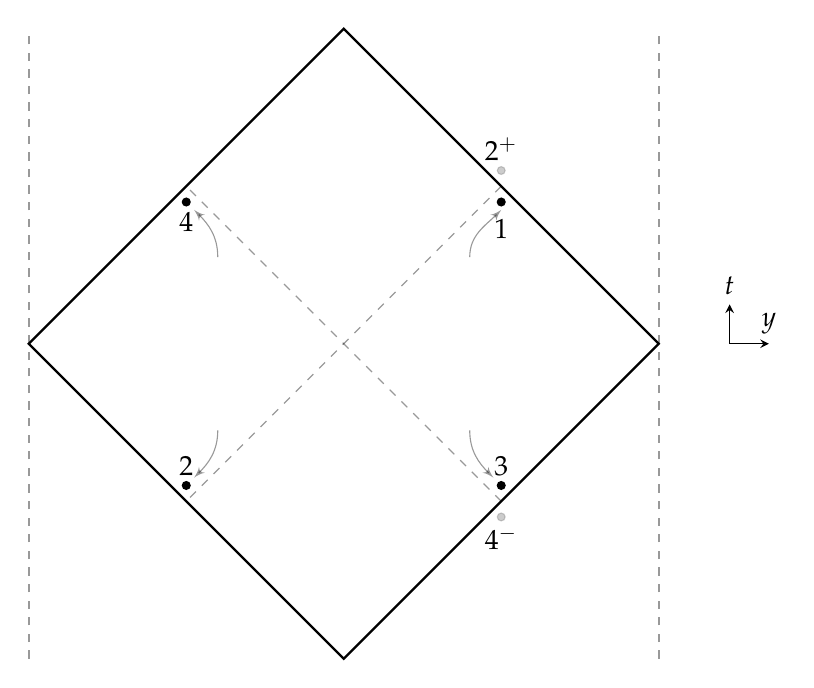
\begin{tikzpicture}
    %draw a square with points at (2,0) (0,2) (0,-2) (-2,-2)
    \draw[thick] (4,0) -- (0,4)  -- (-4,0) -- (0,-4)-- cycle;
    %draw side bisectors
    \draw[dashed,opacity=0.4] (2,2) -- (-2,-2);
    \draw[dashed,opacity=0.4] (2,-2) -- (-2,2);
    %points
    % \node[below] at (0.7,0) {$5$};
    % \draw[fill,black](0.7,0) circle (0.05cm);
    \node[below] at (2,1.7) {$1$};
    \draw[fill,black](2,1.8) circle (0.05cm);
    \node[above] at (2,-1.8) {$3$};
    \draw[fill,black](2,-1.8) circle (0.05cm);
    \node[below] at (2,-2.2) {$4^{-}$};
    \draw[fill,gray,opacity=0.4](2,-2.2) circle (0.05cm);
    \node[above] at (-2,-1.8) {$2$};
    \draw[fill,black](-2,-1.8) circle (0.05cm);
    \node[above] at (2,2.2) {$2^{+}$};
    \draw[fill,gray,opacity=0.4](2,2.2) circle (0.05cm);
    \node[below] at (-2,1.8) {$4$};
    \draw[fill,black](-2,1.8) circle (0.05cm);

    %arrows for Regge 
    \draw[->,opacity=0.4,-latex'] (1.6,1.1) to[out=90,in=225] (2,1.7);
    \draw[->,opacity=0.4,-latex'] (-1.6,1.1) to[out=90,in=-45] (-1.9,1.7);
    \draw[->,opacity=0.4,-latex'] (1.6,-1.1) to[out=270,in=135] (1.9,-1.7);
    \draw[->,opacity=0.4,-latex'] (-1.6,-1.1) to[out=270,in=45] (-1.9,-1.7);

    \draw[opacity=0.4,thick,dashed] (4,-4) -- (4,4);
    \draw[opacity=0.4,thick,dashed] (-4,-4) -- (-4,4);
    %plot axis and label
    \draw[-stealth] (4.9,0) -- (4.9,0.5) node[anchor=south]{$ t $ };
    \draw[-stealth] (4.9,0) -- (5.4,0) node[anchor=south]{$ y $ };
  \end{tikzpicture}
  \caption{Regge limit configuration in the Lorentzian cylinder.}
  \label{fig:ReggeFig}
\end{figure}

\section*{Outline}
This sets the stage for the work in this thesis.
First, we describe the implications of the Regge theory on the CFT data extracted from one loop string theory.
While independent computation of the string theory amplitudes are available mainly in flat space and some $ AdS_3 $ backgrounds, we can employ bootstrap techniques to arrive at a subset of data in $ AdS_5 $.
We can also use the flat space string theory analysis to constrain the amplitude in $ AdS_5 $, since effectively $ AdS_5 $ acts like a one parameter extension of flat space background.

In the latter part, we discuss the generalization of the Conformal Regge theory to many point correlation functions.
We first review the case of multi-Regge limit in the many particle scattering amplitude in quantum field theories.
Then, we discuss its generalization to the conformal field theories.


\section{Kinematics of conformal field theory}
Now, we turn to a detailed introduction of the theories considered in this thesis.

In this section, we discuss the kinematics of conformal field theory.
Conformal field theories in $ d $ dimensions are a class of quantum field theories with additional symmetries that are not present in the standard quantum field theories.
In the Euclidean space, the conformal field theories are invariant under the Euclidean conformal group, $ SO(d+1,1) $, while in the Lorentzian space they are invariant under the Lorentzian conformal group, $ SO(d,2) $.
The generators of the Euclidean conformal group can be written in terms of the spacetime derivative $ \partial_{\mu} $ as
\begin{align}
  \text{Translations}                      &  & P_{\mu} & = \partial_{\mu}                                                            ,  \\
  \text{Rotations}                         &  & M_{\mu} & =  i\left( x_\mu \partial_\nu - x_\nu \partial_\mu \right)                   , \\
  \text{Dilatations}                       &  & D       & = i x^\nu \partial_\nu                                                       , \\
  \text{Special conformal transformations} &  & K_{\mu} & = i\left( 2x_\mu \left( x^\nu \partial_\nu \right) -x^2 \partial_\mu \right)
  .
\end{align}
However, some of these generators act nonlinearly on the spacetime points.
Therefore, it is useful to consider `Embedding space':
\begin{align}
  X^A = \left( \frac{1+x^2}{2},\frac{1-x^2}{2},x^\mu  \right)  ,
\end{align}
with the signature $ \left( -,+,\dots,+ \right) $.
The Euclidean conformal group acts linearly on $ X $.
This simplifies several calculations, for instance, the inner product in the physical space given by  $ \left( x_\mu -y_\mu \right) \left( x_\nu - y_\nu \right) \delta^{\mu\nu} $ becomes $ X\cdot Y =X_A Y_B \eta^{A B} $.
Here, $ X,Y $ are respective embedding coordinates for $ x,y $.
This allows us to identify the dependence on the spacetime variables of the correlations functions.

The physical observables in conformal field theory are the correlation functions of the local operators in the theory.
The local operators are characterized by quantum numbers of the generators of the conformal group.
We consider a special set of operators, called `primary' operators.
They are precisely the operators which are annihilated by special conformal transformations $ K_\mu O =0 $.
All the other operators are `descendants' of one of these operators, namely, they are of the form: $ \left( P_\mu \right)^n O $.
In particular, the operators are labeled by the quantum numbers for dilatations: $ \Delta $  and rotations: $ \lambda $, a Young tableux diagram for the representation.
Thus, a representation of the conformal group $ R $ is labeled by $ \left( \Delta,\lambda \right) $.
In the simple case of symmetric traceless representation, $ \lambda $ can be replaced by the number of boxes in $ \lambda $, representing the spin.

Two and three points correlation functions of the primary scalars, the primary operators with spin $ 0 $ and scaling dimensions $ \Delta_i $ can be written in terms of the embedding space as follows \cite{Poland:2018epd},
\begin{align}
  \langle\phi\left( X \right) \phi\left( Y \right) \rangle                      & =\frac{\delta_{\Delta_1 \Delta_2}}{\left( X \cdot Y \right)^{\Delta_1}} ,                                                        \\
  \langle\phi\left( X \right) \phi\left( Y \right)\phi\left( Z \right)  \rangle & =\frac{c}{\left( X \cdot Y \right)^{\alpha_{123}}\left( Y \cdot Z \right)^{\alpha_{231}}\left( Z \cdot X \right)^{\alpha_{132}}}
  .
\end{align}
We have chosen the normalization of the operators such that the two point function numerators are $ 1 $.
The numerator in the three point function, $ c $,  is called `operator product expansion coefficient' (OPE coefficient).
We have also used $ \alpha_{ijk} = \left( \Delta_i + \Delta_j - \Delta_k \right)/2 $ .

The set of representations $ R $'s of the local primary operators and their respective OPE coefficients $ c_{R_1,R_2, R_3} $ consitute a useful characterization of the observables in conformal field theory, called `\emph{CFT data}'.

While it is easy to see that the spactime dependence of the two and three point functions are fixed by the conformal invariance, the situation changes for higher point functions.
The four point function is not fixed by the conformal invariance because there exist conformal invariant `cross ratios'
\begin{align}
  U=\frac{X_{12} X_{34}}{X_{13} X_{24}}, \,\, & V= \frac{X_{14}X_{23}}{X_{13}X_{24}}.
  \label{eq:crossRatios}
\end{align}
The dependence on these cross ratios can not  be fixed by conformal invariance alone.
This allows us to write the four point correlation function of identical scalars as
\begin{align}
  \langle\phi\left( X_1 \right) \phi\left( X_2 \right)\phi\left( X_3 \right) \phi\left( X_4 \right) \rangle = \frac{1}{X_{12}^\Delta X_{34}^\Delta} A\left( U,V \right).
\end{align}
$ A $ denotes an unknown function of cross ratios.
However, since the operators $ \phi $'s are identical, their correlation function is permutation invariant.
It is easy to see that this leads to a constraint on $ A $, namely \cite{Poland:2018epd}
\begin{align}
  A\left( U,V \right) \left( \frac{V}{U} 	 \right)^\Delta & = A\left( V,U \right) .
\end{align}
This is called as the `\emph{crossing constraint}'.

The goal of conformal bootstrap is to use the consistency conditions of the conformal field theory to constrain the CFT data.
In particular, we use consistency of the four point function to arrive at constraint on the lower point functions.

In conformal field theories, one can use `\emph{operator product expansion}'.
\begin{align}
  \phi\left( x \right) \phi\left( y \right) = \sum_{\textit{primary } O} c_{\phi \phi O}\left( x-y,\partial_{x-y} \right) O\left( y \right)	.
\end{align}
Unlike a generic quantum field theory, this expansion has a finite radius of convergence.
This is an operator level statement and therefore is valid in all correlation functions.
In particular, it can be used to write down a four point correlation function in terms of the lower point correlation function.
\begin{align}
  \langle\phi\left( x \right) \phi \left( y \right)\times \phi \dots \phi \rangle &
  = \sum_{\textit{primary } O} c_{\phi \phi O}\left( x-y,\partial_{x-y} \right) \langle O\left( y \right) \phi \dots \phi\rangle	.
\end{align}
Note that the right hand side correlation function has fewer operator insertions than the left hand side correlation function.

In this thesis, we will concern outselves with unitary quantum field theories.
Unitarity of conformal field theory, which is also a quantum field theory imposes constraint on the CFT data.
This leads to a nontrivial constraint on the four point correlation function when expanded in terms of the lower point correlation functions.

These constraints are used in the program of Euclidean conformal bootstrap.
However, in this thesis, we are mainly concerned with the constraints coming from the Lorentzian consistency of the conformal field theory.
In the following, we discuss the necessary tools to discuss correlation function in the Lorentzian setup and its relation to the Euclidean correlation function.


\section{Wightman functions}
In this section, we discuss the Wightman functions and their properties.
The Wightman functions are useful in going back and forth between the properties of Lorentzian correlators and their Euclidean counterparts.
We closely follow the discussion in \cite{Hartman:2015lfa}.

For concreteness, we consider the correlation function of four identical scalars $ \phi $.
First, we discuss the Euclidean correlation function in the Euclidean space with time direction denoted by $ \tau $ and space directions labelled by $ y_i $.
As discussed before, such a correlation function is fixed up a function, $ A $, of two cross ratios $ U,V $.
We define a rewriting of the cross ratios $ U  = z \bar{z}$ and $ V = \left( 1-z \right) \left( 1-\bar{z} \right) $.
This rewriting is especially useful when we use the conformal symmetry to fix three out of the four points to be at $ 0,1,\infty $.
The point that is not fixed can be brought to the same plane as the other three points by a conformal transformation.
The location of this point is precisely $ z $ in the complex plane $i \tau + y $ .
We choose the second point to be written in terms of $ z $.
Thus, the Euclidean correlation function is given by $ A\left( z,\bar{z}=z^* \right) $.
Note that in the Euclidean setup, we have $ \bar{z} = z^* $, since $ \tau $ is real.
Now, we would like to discuss the procedure to convert this correlation function to a Lorentzian correlation function.
In this case, the Euclidean time becomes purely imaginary.
Therefore, $ z,\bar{z} $ are no longer complex conjugates of each other, but are in fact complex numbers.

In the Lorentzian setup, commutator of two operators spacelike separated.
\begin{align}
  \left[ O_1\left( x_1 \right),O_2\left( x_2 \right) \right] = 0 &  & x_1 \approx x_2.
\end{align}
In particular, if we move the point $ x_2 $ from the region spacelike separated from $ x_1 $ to the region timelike separated from $ x_1 $, the commutator encounters a jump.
This jump is reminiscant of branch cut behaviour.
In fact, the correlation function in the Lorentzian setup is given by an appropriate analytic continuation of the Euclidean correlation function.
One expects that the function $ A $ admits a branch cut when two of the points in the correlation function become lightlike separated.

We study the correlation function by first starting in the Euclidean setup with points fixed at
\begin{align}
  x_1 & = \left( 0,0,\dots,0 \right), & x_2 & = \left( \tau_2,y_2,\dots,0 \right), \nonumber \\
  x_3 & = \left( 0,1,\dots,0 \right), & x_4 & = \left( 0,\infty,\dots,0 \right)
  .
\end{align}
Now, the idea is to move the second point away from the Euclidean space positions to Lorentzian space positions.
This involves a Wick rotation $ \tau \rightarrow i t $ with appropriate $ i\epsilon $ prescription.
While doing so, one can encounter a branch cut due to the presence of the lightcones in the Lorentzian spacetime.
It is easy to see that the location of the branch cuts in $ \tau_2 $ is as depicted in figure \ref{fig:cutsInTau}.
Going from Euclidean to Lorentzian, the value of $ \tau_2 $ goes from a real number to a purely imaginary number.

One can study the implications of this branch cuts on the correlation function as a function of the cross ratios.
This branch cuts implies a branch cut in the correlation function at $ z,\bar{z} \in \left( 1,\infty \right)  $.

\begin{figure}[t]
  \centering
  \begin{tikzpicture}
    %name
    \draw[] (-5.2,3) -- (-5.2,2.5) -- (-5.7,2.5);
    \node[left] at (-5.2,2.8) {$\tau_2$};
    %axis
    \draw[->,opacity=0.3,-latex'] (0,0) -- (-5,0);
    \draw[->,opacity=0.3,-latex'] (0,0) -- (0,3);
    \draw[->,opacity=0.3,-latex'] (0,0) -- (0,-3);
    \draw[->,opacity=0.3,-latex'] (0,0) -- (5,0);
    %drawing points 
    \draw[fill=black] (0,1) circle (0.05);
    \draw[fill=black] (0,2) circle (0.05);
    \draw[fill=black] (0,-1) circle (0.05);
    \draw[fill=black] (0,-2) circle (0.05);
    %labelling
    \node[left] at (-0.4,1) {$i(y_2-y_1)$};
    \node[right] at (0,2) {$i(y_3-y_2)$};

    \node[left] at (0,-2) {$-i(y_3-y_2)$};
    \node[left] at (0,-1) {$-i(y_2-y_1)$};
    %drawing cuts
    \draw[red,opacity=0.8,dashed] (0,1) -- (-0.3,3);
    \draw[red,opacity=0.8,dashed] (0,2) -- (-0.3,4);

    \draw[red,opacity=0.8,dashed] (0,-2) -- (0.3,-4);
    \draw[red,opacity=0.8,dashed] (0,-1) -- (0.3,-3);
    \draw[black,opacity=0.8] (3,0) -- (-0.3,0.5);
    \draw[black,opacity=0.8] (3,0) -- (0,2) -- (-0.3,0.5);
  \end{tikzpicture}
  \caption{Location of cuts in the complex $\tau$ plane.
    The grey lines are the possible path, with or without crossing the branch cuts.}
  \label{fig:cutsInTau}
\end{figure}

This exotic branch structure allows us to probe more constraints on the correlation function.
In particular, there are constraints coming from the Lorentzian consistency which are hard to see from the Euclidean CFT understanding.
Euclidean correlation functions are simplified in the `OPE limit', when two of the points are colliding.
This is a somewhat singular limit, but allows us to study the correlation function analytically.
This corresponds to $ z \rightarrow 0,1 \text{ or }  \infty $ limit in the correlation function $ A $.
The complicated structure of cuts allows us access to a bigger set of singular structure of the correlation function.
We can choose to cross some of these branch cuts \emph{before} taking the limit $ z \rightarrow 0,1 \text{ or }  \infty $.
Study of such limits of the correlation function is called `Regge theory'.

An important aspect of this limit is that we access the sheets of the correlator which are not principal.
Principal sheet corresponds to the Euclidean configurations.
However, we can use many paths to go away from this region.
For instance, consider the configuration of the correlation function when $ 2 > 3  $ and $ 1 < 4 $ whereas all the other pairs are spacelike separated.
This allows us to reach the following Wightman functions,
\begin{align}
   & \langle \phi\left( x_4 \right)\phi\left( x_1 \right)\phi\left( x_2 \right)\phi\left( x_3 \right) \rangle, \nonumber \\
   & \langle \phi\left( x_4 \right)\phi\left( x_1 \right)\phi\left( x_3 \right)\phi\left( x_2 \right) \rangle, \nonumber \\
   & \langle \phi\left( x_1 \right)\phi\left( x_4 \right)\phi\left( x_2 \right)\phi\left( x_3 \right) \rangle, \nonumber \\
   & \langle \phi\left( x_1 \right)\phi\left( x_4 \right)\phi\left( x_3 \right)\phi\left( x_2 \right) \rangle
  .\end{align}
It is easy to see that in this configuration, $ 1,2 $ OPE converges on the right vacuum in the second Wightman function as $ 1 $ can be commuted with $ 3 $.
Similarly, it converges on the left vacuum in the third Wightman function since $ 2 $ and $ 4 $ are spacelike separated.
However, the first and the fourth Wightman functions do not have a convergent $ 1,2 $ OPE.
Therefore, they can not be arrived at by naive analytic continuation of the Euclidean correlation function without encountering monodromy.
One can track the path in the cross ratio space $ z,\bar{z} $ during this analytic continuation of $ x_i $.
It amounts to taking $ \bar{z} $ going across the cut $ \bar{z} = 1 $ in the clockwisek or counterclockwise direction, for the fourth and the first Wightman function, respectively.
Thus, these Wightman functions are $ A^\circlearrowleft,A,A,A^\circlearrowright $, respectively.

These four Wightman functions can be combined to write an interesting quantity, $ \text{dDisc} $.
This quantity serves as a generalization of imaginary part of the scattering amplitude, in a sense that it is manifestly positive.
It is also an important quantity since the analogue of the inversion formula feeds on it.
Formally, it is defined as
\begin{align}
  \text{dDisc} A \left( z,\bar{z} \right)  =
  \cos \left( \pi\left( a+b \right) \right) A \left( z,\bar{z} \right)
  -\frac{1}{2}\left[
  e^{i\pi \left( a+b \right)}A^{\circlearrowright}\left( z,\bar{z} \right)
  +e^{i\pi \left( a+b \right)} A^{\circlearrowleft}\left( z,\bar{z} \right)
  \right]
  .\end{align}
Here, we have used $ a = \frac{\Delta_2 - \Delta_1  }{2}, \, b = \frac{\Delta_3 - \Delta_4 }{2}$.
The phase factors come from changing the time ordering of the unequal operators.
For equal scalars, the phase factors become $ 1 $.
Incidently, this quantity also admits an elegent formulation in terms of `double commutator',
\begin{align}
  \langle \left[ \phi_1, \phi_4 \right] \left[ \phi_2,\phi_3  \right]\rangle & =
  x_{12}^{-2\Delta_\phi}
  x_{34}^{-2\Delta_\phi}
  \text{dDisc}\left( A \right)
  .\end{align}







\section{Regge theory}
We discuss some aspects of Regge theory in this section.
Regge theory concerns the study of the correlation function in the `Regge limit'.
This is a generalization of the `Regge limit' in the scattering amplitudes, which concerns the high energy limit.

Consider the case of two to two scattering amplitudes.
They are described in terms of the momenta of the external particles, $p_1, p_2, p_3, p_4$.
However, due to conservation of momenta as well as Lorentz invariance of the theory, they depend only on the two invariants, $s =-\left( p_1 + p_2 \right)^2$ and $ t =-\left( p_1 + p_3 \right)^2 $.
Regge limit concerns an extreme high energy scattering limit wherein $ s $ is large while $ t $ is fixed.

Analogously, the correlation functions of four operators in a Lorentzian conformal field theory depend on two cross ratios, $ U,V $, defined in equation \ref{eq:crossRatios}.
In terms of these cross ratios, one can consider various limits.
One can consider the `OPE limit' where two of the four operators approach each other.
This amounts to $ U \rightarrow 0, V \rightarrow 1 $ with $ \left( V-1 \right)/\sqrt{U} $ fixed.
The latter, $ \xi $, is the analogue of the scattering angle in the S-matrix case.
One can also consider the limit where one of the operators approach the lightcone of the other.
This is called the `lightcone limit'.
This amounts to $ U\rightarrow 0 $ for any $ V $.

In the Regge limit, we are concerned with a certain generalization of the OPE limit.
As described in the previous section, the correlation function has interesting analytic structure.
Therefore, one has a lot more freedom to consider the generalization of the lightcone limit.
Several lightcones of the form $ x_{ij}^2 = 0 $ are related to nontrivial analytic structure such as branch points and branch cuts in terms of the cross ratio space $ U,V $.
Regge limit concerns the OPE limit, however, it is taken after crossing the cuts in $ V $ cross ratio at $ V = 1 $.

In the following, we study the effect of this limit on the correlation function of four operators, $ \phi $.
Using conformal symmetry, we first represent the correlation function in terms of the cross ratios, $ A\left( U,V \right) $.
It admits an expansion in terms of certain kinematical functions of cross ratios called `conformal blocks', denoted by $ G $.
\begin{align}
  A\left( U,V \right) & = \displaystyle\sum_{O} \lambda_{\phi \phi O}^2 G_{O}\left( U,V \right)
\end{align}
These objects are defined for each primary $ O $ and come from summing over all the descendants of a given primary $ O $.
Each primary is a representation of the Euclidean conformal group, and therefore labeled by scaling dimensions, $ \Delta $ and the representation of the rotation group, $ \Lambda $.
For the symmetric traceless representation of the rotation group, it is just the spin quantum number.
While these are interesting objects themselves, it is useful to rewrite the expansion in terms of `conformal partial waves', $ F_{O} $.
Similar to the S-matrix partial waves, these partial waves have a well defined orthogonality properties.
They can be expressed as a linear combination of the conformal block as follows
\begin{align}
  F_{O} = G_O + \frac{\kappa_{\tilde{O} }}{ \kappa_{O}} G_{\tilde{O}}
  .\end{align}
The expressions for $ \kappa $ can be found in \cite{Costa:2012cb}.
The orthogonality holds for the operators on the `principle series representations'.
These are operators whose scaling dimensions is $ \nu = d/2 + i \mathbb{R} $.
The orthogonality relation can be written in terms of some weight function $ \mu $ as \cite{Caron-Huot:2017vep}
\begin{align}
  \int dU dV \, \mu\left( U,V \right) F_{O}\left(U,V \right) F_{O'}\left(U,V \right) = n_{O} \delta_{O \, O'}
  .
\end{align}

Since these partial waves form a complete basis, we can consider the partial wave expansion in spacetime dimensions $ d = 2 h $ \cite{Costa:2012cb, Caron-Huot:2017vep},
\begin{align}
  A\left( U,V \right) & = \displaystyle\sum_{J} \displaystyle\int_{h+ i \mathbb{R}}
  \frac{
    d\nu}{2\pi i }
  b_{\nu,J} F_{\nu,J}\left( U,V \right).                                                    
\end{align}
Here, we have introduced the `OPE function' $ b_{\nu,J} $
\begin{align}
  b_{\nu,J}           & =\frac{ \lambda_{\phi \phi O}^2}{\nu^2 - \left( \Delta-h \right)^2}
.\end{align}
It is an analytic function of $ \nu $ with poles at the location of the physical operators.

We discuss the analytic structure of the correlation function in the Regge limit as a function of $ V $.
The lightcones result in two branch point singularities at $ V = 1 $ and $ V= \infty $.
To separate them, we write a decomposition of the correlator \cite{Costa:2012cb} as follows
\begin{align}
  A & =
  A^{+} +
  A^{-}
  ,\end{align}
such that the first one has no nontrivial monodromy around $ V =1  $, whereas the later has no nontrivial monodromy around $ V= \infty $.
Corresponding to each, we define the `signatured OPE function', $ A^{\theta = \pm} $.
They are the coefficient of the partial wave expansion of the signatured correlator
\begin{align}
  A^{\theta }\left( U,V \right) & = \displaystyle\sum_{J} \displaystyle\int_{h+ i \mathbb{R}}
  \frac{
    d\nu}{2\pi i }
  b_{\nu,J}^{\theta} F_{\nu,J}\left( U,V \right)
  .
\end{align}
They get contributions from even and odd spins, respectively.
It is now known that these `signatured OPE functions' are also analytic functions of $ J $ \cite{Caron-Huot:2017vep}.
Thus, even and odd spins form `Regge trajectories'.
These are interesting analytic manifolds with analyticity in $ J $.

First, we discuss the limiting behaviour of the conformal partial wave in the Regge limit.
This limit can be written as $ \sigma \rightarrow 0 $ with fixed $ \xi  $ where we use
\begin{align}
  \sigma^2 = z \bar{z}, \, &  & \xi =
  \frac{1}{2} \left(
  \sqrt{\frac{z}{\bar{z}}} + \sqrt{\frac{\bar{z}}{z}}
  \right)
  .\end{align}
As we will discuss later in the thesis, the Regge limit of the partial wave in generic dimensions is $ \sigma^{1-J}  $.
Thus, the leading contribution to the correlator comes from the operators with higher spins.
However, operators with arbitrarily large spin appear in the spectrum.
To make sense of this sum over spins, we use the techniques from complex analysis.


We will use the analyticity in spin in the following.
We discuss the evaluation of the correlator in the Regge limit described above.
First, we replace the sum over spins by a contour integral over the positive real line, shown in blue in \cref{fig:polesInJ}.
Then, we consider deforming this contour to the red contour.
In the process, we pick any pole that we may encounter \cite{Costa:2012cb}.
This pole is called `the pomeron'.
Furthermore, the integral over $ \nu $ can also be performed in the saddle point approximation in certain cases \cite{Costa:2017twz}.
Thus, the leading behaviour of the correlator in the Regge limit is given by $ \sigma^{1-j^{*}}  $, where $ j^{*} $ is the location of the circled pole in \cref{fig:polesInJ}  evaluated at the saddle point in the $ \nu $ integral.


\begin{figure}[t]
  \centering

  \resizebox{0.6\textwidth}{!}{
    \begin{tikzpicture}
      %name
      \draw[] (-1.2,3) -- (-1.2,2.5) -- (-1.7,2.5);
      \node[left] at (-1.2,2.8) {$J$};
      %axis
      \draw[->,opacity=0.3,-latex'] (0,0) -- (-1.5,0);
      \draw[->,opacity=0.3,-latex'] (0,0) -- (0,3);
      \draw[->,opacity=0.3,-latex'] (0,0) -- (0,-3);
      \draw[->,opacity=0.3,-latex'] (0,0) -- (5.8,0);
      %drawing points 
      \draw[fill=black] (0,0) circle (0.05);
      \draw[fill=black] (1,0) circle (0.05);
      \draw[fill=black] (2,0) circle (0.05);
      \draw[fill=black] (3,0) circle (0.05);
      \draw[fill=black] (4,0) circle (0.05);
      \draw[fill=black] (5,0) circle (0.05);
      \draw[fill=black] (0.3,1) circle (0.05);

      %drawing circles
      \draw[<-,line width=0.7,blue] (0.2,0) to[out=90,in=0] (0,0.2) to[out=180,in=90] (-0.2,0) to[out=-90,in=180] (0,-0.2) to[out=0,in=-90] (0.2,0);
      \draw[<-,line width=0.7,blue] (1.2,0) to[out=90,in=0] (1,0.2) to[out=180,in=90] (0.8,0) to[out=-90,in=180] (1,-0.2) to[out=0,in=-90] (1.2,0);
      \draw[<-,line width=0.7,blue] (2.2,0) to[out=90,in=0] (2,0.2) to[out=180,in=90] (1.8,0) to[out=-90,in=180] (2,-0.2) to[out=0,in=-90] (2.2,0);
      \draw[<-,line width=0.7,blue] (3.2,0) to[out=90,in=0] (3,0.2) to[out=180,in=90] (2.8,0) to[out=-90,in=180] (3,-0.2) to[out=0,in=-90] (3.2,0);
      \draw[<-,line width=0.7,blue] (4.2,0) to[out=90,in=0] (4,0.2) to[out=180,in=90] (3.8,0) to[out=-90,in=180] (4,-0.2) to[out=0,in=-90] (4.2,0);
      \draw[<-,line width=0.7,blue] (5.2,0) to[out=90,in=0] (5,0.2) to[out=180,in=90] (4.8,0) to[out=-90,in=180] (5,-0.2) to[out=0,in=-90] (5.2,0);

      \node[below] at (0.2,-0.1) {$0$};
      \node[below] at (1.2,-0.1) {$1$};
      \node[below] at (2.2,-0.1) {$2$};
      \node[below] at (3.2,-0.1) {$3$};
      \node[below] at (4.2,-0.1) {$4$};
      \node[below] at (5.2,-0.1) {$5$};
      %main contour before deforming
      \draw[->,line width=0.7,red] (0.5,1) to[out=90,in=0] (0.3,1.2) to[out=180,in=90] (0.1,1) to[out=-90,in=180] (0.3,0.8) to[out=0,in=-90] (0.5,1);
      \draw[->,line width=0.7,red,-latex'] (-1,-3) -- (-1,3);

      \node[above right] at (0.3,1.1) {$j(\nu)$};
    \end{tikzpicture}
  }
  \caption{Location of poles in the complex $ J$ plane.
    In blue, the spins in the Euclidean conformal field theory are shown.
    $ j\left( \nu \right)  $ denotes the special poles in the complex plane that dominates the Regge limit of the correlator.}
  \label{fig:polesInJ}
\end{figure}

\section{An inversion formula}
In the previous section, we discussed the representation of the conformal correlator in terms of the CFT data via conformal block expansion.
The goal of this section is to discuss the `inverse' of that expansion, called as an `inversion formula'.

First, we present a toy model from a single variable complex analysis that captures the essence of the main formula.
Consider an analytic function $ A $ of a complex variable $ w $.
We would like to consider its Taylor series expansion around $ w = 0 $,
\begin{align}
  A\left( w \right) & = \sum_{J= 0 }^{\infty} a_J w^J
  .
\end{align}
A priori, the expansion coefficients $ a_J $ are independent of each others.
In other words, one can change, say, $ a_{134} $ by a small amount without changing any other $ a_J $.

Now, we take an alternate point of view at the same expansion formula.
It uses the orthogonality of the power laws, playing the role of partial waves
\begin{align}
  \oint dw \, w^a w^b = \delta_{a,-1-b}
  .
\end{align}
This is essentially the Cauchy formula for the contour circling the origin.
The Euclidean inversion formula implied by this is
\begin{align}
  a_J  =  \oint \frac{dw}{2\pi i} \, w^{-1-J} A\left( w \right)
  .
\end{align}
If we assume that the function $ A $ has a nice behavior at $ \infty $, we can deduce more properties of the function $ a_J $.
Let us say $ A $ is bounded as
\begin{align}
   & A\left( w \right) \leq 1 & w \rightarrow \infty
  .\end{align}
Naively, this appears impossible to achieve as all the power laws $ w^J $ blow up at large $ w $, for $ J>1 $.
Thus, imposing the boundedness constraint provides highly nontrivial relations among all $ a_J $'s.

The best way to make use of this is to consider the contour deformation of the orthogonality relation, as in \cref{fig:wcontourdeformatoin}.
Assume that the function has a cut on the positive real axis starting at $ 1 $.
Then, the blue contour can be deformed into the red contour.
Boundedness at infinity allows us to drop the circle at infinity in the \cref{fig:wcontourdeformatoin}.
The only nontrivial ingredient is the evaluation of the integrand on the two sides of the cut.
This is essentially the \emph{discotinuity} of the function $ A $,
\begin{align}
  \text{Disc}\left[ A\left( w \right) \right] \equiv A\left( w + i \epsilon \right) - A\left( w - i \epsilon \right)
  .\end{align}
In terms of this discotinuity, one can write the formula for $ a_J $,
\begin{align}
  a_J & = \frac{1}{2\pi i } \int_{1}^{\infty}\frac{dw }{w^{J+1}} \text{Disc} \left[ A\left( w \right) \right]
  \label{eq:toyInversion}
  .\end{align}
Note that, we have dropped the circle at infinity assuming the boundedness behavior.
However, the power law $ w^{J} $ for $ J = 0  $ is already bounded in the large $ w $ limit.
Thus, the \cref{eq:toyInversion} does not constrain the coefficient $ a_0 $ and the \cref{eq:toyInversion} is valid only for $ \operatorname*{Re} J > 0 $.

Let us consider a concrete example of a function $ A = \log \left( 1-w \right) $.
It's discotinuity across the cut is simply a constant, $ -2 \pi i $.
This leads to an analytic formula for $ a_J $,
\begin{align}
  a_J  = -\frac{1}{J}, & \, \, \text{Re} \left( J \right) >0
  .\end{align}
The analyticity in the variable $ J $ is best visualized as in the \cref{fig:toyAnalyticity}.

The goal of Lorentzian inversion formula is to produce a formula that displays the analyticity in spin in conformal field theories.
As we showed the analyticity in $ J $, the example from the single variable complex analysis serves as a good toy model of the Lorentzian inversion formula.


\begin{figure}[t!]
  \centering
  \begin{tikzpicture}
    %name
    \draw[] (-2.2,3) -- (-2.2,2.5) -- (-2.7,2.5);
    \node[left] at (-2.2,2.8) {$w$};
    \node[below right] at (1,0) {$1$};
    % \node[below right] at (3,0) {$\infty$};
    %axis
    \draw[->,opacity=0.3,-latex'] (0,0) -- (-3.5,0);
    \draw[->,opacity=0.3,-latex'] (0,0) -- (0,3.5);
    \draw[->,opacity=0.3,-latex'] (0,0) -- (0,-3.5);
    \draw[->,opacity=0.3,-latex'] (0,0) -- (3.5,0);
    %circle
    \draw[blue,dashed] (0,0) circle (1);
    \draw[red,dashed] (0,0) circle (3);
    \draw[red,snake it] (1,0) -- (3,0);
  \end{tikzpicture}
  \caption{Contour deformation for the toy model in single variable complex analysis. Analyticity implies that the contour integral over the region between blue and red contours is zero.}
  \label{fig:wcontourdeformatoin}
\end{figure}

\begin{figure}[t!]
  \centering
  % \includegraphics*[width=\textwidth]{Figures/AnalyticJ.jpeg}
  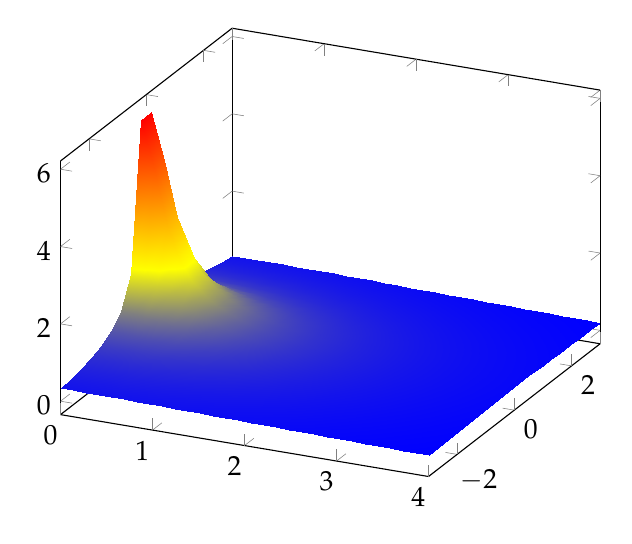
\begin{tikzpicture}
    \begin{axis}
      \addplot3 [
        domain=0:4,
        domain y = -3:3,
        samples = 30,
        samples y = 18,
        surf,
        % fill= yellow,
        shader = interp] {1/(sqrt(x^2+y^2))};
      % \addplot coordinates {(1,0,1)};
    \end{axis}
  \end{tikzpicture}
  \caption{We plot the absolute value of $ a_J $ with respect to real and imaginary part of $ J $.
    The orthogonality relation would only lead to the points corresponding to the positive integer values of $ J $.
    However, analyticity in $ J $ suggests that a more appropriate way to think about $ a_J $ is the whole colored manifold, rather than just the isolated points.
  }
  \label{fig:toyAnalyticity}
\end{figure}

\subsection*{Casimir equation}
Our goal is to introduce the Lorentzian inversion formula in a simple setting of two dimensions.
Most of the technical details are analogous in the generic dimensions.
We list the analogies with the toy model discussed above in \cref{ta:analogies}.

\begin{table}[ht ]
  \centering\begin{tabular}{c|c|c }
                                                                   & Toy model & CFT                                                      \\
    \hline
    Orthogonal partial wave                                        & $ w^{J} $ & $ F_{h + i \nu,J} \left( u,v \right) $                   \\
    Orthogonality relation                                         &
    $\oint \frac{dw}{2 \pi i} \, w^{J} w^{J'} = \delta_{-1-J,J'} $ &
    $ \int du \, dv \, \omega \, F_{h + i \nu,J}   \, F_{h + i \nu',J}  =\left(  n_{\nu,\nu'} \delta_{\nu,\nu'} + \text{shadow} \right) $ \\
    Coefficient function                                           & $ a_{J} $ & $ c_{\nu,J} $
  \end{tabular}
  \caption{Analogy between the toy model and the conformal field theories}
  \label{ta:analogies}
\end{table}

We summarize some useful properties of conformal blocks here \cite{Dolan:2003hv}.
The operator product expansion of two external operators can be arranged into families of operators such that all the operators are either a primary or its descendant
\begin{align}
  \phi \times \phi & = \sum_{O} \lambda_{O} O
  .\end{align}
This allows us to write the correlator as a sum over blocks with contribution coming from this primary
\begin{align}
  A \left( u,v \right) & = \sum_{O} \, \lambda_{O}^2 G_{O} \left( u,v \right)
  .\end{align}

However, we can use conformal symmetry to characterize the blocks in a different way.
Since they are functions of two variables $ u,v $, or alternatively, of $ z, \bar{z} $, they can be written as solutions to the differential equation, called the Casimir equation
\begin{align}
  C_2 \, G_{\Delta,J} & = c_2 \, G_{\Delta,J}
  .\end{align}
Here, we have used the notation that $ a = \left( \Delta_2 - \Delta_1 \right)/2 $ and $ b = \left( \Delta_3 - \Delta_4 \right)/2 $,
\begin{align}
  \label{eq:CasimirEq}
  C_2   & = D_z  + D_{\bar{z}} + \left( d-2 \right) \frac{z \bar{z}}{z - \bar{z}} \left[ \left( 1-z \right) \partial_{z} - \left( 1 - \bar{z} \right) \partial_{\bar{z}} \right] ,\nonumber \\
  c_2   & = \frac{1}{2} \left[ J\left( J+d-2 \right)+ \Delta\left( \Delta-d \right) \right]\nonumber                                                                                        \\
  D_{z} & = z^2 \partial_z \left( 1-z \right) \partial_z - \left( a+b \right)z^2 \partial_z -  a b z
  .\end{align}
For equal external scalars, these simplify due to $ a = b = 0 $.
The solutions to this equation admit several symmetries which they inherit from the Casimir eigenvalue, which correspond to swapping two elements in the following tuples,
\begin{align}
  \label{eq:swaps}
  \left( J \leftrightarrow 2-d-J \right),
  \quad
  \left( \Delta \leftrightarrow d-\Delta \right),
  \quad
  \left(\Delta  \leftrightarrow 1-J \right)
  .\end{align}

It can be seen that the differential equation in \cref{eq:CasimirEq} admits a power law solution in $ z , \bar{z} $ if we strip out a pure power law as a leading behavior.
Thus, we define a `pure' solution to the differential equation as the solution with the boundary condition
\begin{align}
  g_{\text{pure},\Delta,J}\left( z,\bar{z} \right) & =	z^{\frac{\Delta-J}{2}} \bar{z}^{\frac{\Delta + J}{2}} \left( 1 + \text{subleading power laws} \right)  \nonumber \\
                                                   & 0 \ll z \ll \bar{z} \ll 1
  .\end{align}
Thus, there are $ 8 $ solutions to the differential equation of the form $ g_{\text{pure},\Delta,J}$.
Each of which can be obtained by doing the swaps in \cref{eq:swaps} to the main pure solution $ g_{\text{pure},\Delta,J} $.
A general solution to the differential equation is a linear combination of these $ 8 $ solutions.

Two of the most important solutions are called the conformal block $ G_{\Delta,J} $ and the conformal partial wave $ F_{\Delta,J} $.
Conformal block resums the contribution of the primary and its descendant, whereas partial wave is a linear combination of the conformal block and its `shadow', $ \Delta \rightarrow d-\Delta $.
In two dimensions, the conformal block can be written in a closed form in terms of the hypergeometric functions
\begin{align}
  G_{\Delta,J } & = \frac{1}{1+\delta_{J,0}} \left[ k_{\Delta-J}\left( z \right) k_{\Delta+J}\left( \bar{z} \right) + k_{\Delta-J}\left( z \right)  k_{\Delta+J}\left( \bar{z} \right)  \right]
  .\end{align}
The two terms here are equivalent to $ g_{\text{pure}} $.
Here, we have defined
\begin{align}
  k_{\beta}^{a,b}\left( z \right) & = z^{\beta/2}
  {{}_{2}F_{1}\left(\genfrac..{0pt}{}{\beta/2+ a , \beta/2 +b}{\beta};z\right)}
  .\end{align}
The conformal blocks in general dimensions can be written in a similar fashion.
We use the shorthand $ g $ to denote $ g_{\text{pure}} $.
\begin{align}
  G_{\Delta,J} & = g_{\Delta,J} + \frac{\Gamma\left( J+d-2 \right)  \Gamma\left( -J - \frac{d-2}{2} \right)	}{ \Gamma\left( J+ \frac{d-2}{2} \right) \Gamma\left( -J \right)}  g_{\Delta, 2-d-J}
  .\end{align}

A more useful object for our purpose is the conformal partial wave, $ F_{\Delta,J} $, as it admits nice orthogonality properties.
It is defined as the unique linear combination of the conformal block, $ G_{\Delta, J} $, and its shadow, $ G_{d-\Delta, J} $, that is single valued in the Euclidean signature.
Here, Euclidean signature means $ \bar{z} = z^{*} $,
\begin{align}
  \label{eq:partialWaveIntro}
  F_{\Delta,J} & =\frac{1}{2}\left[  G_{\Delta,J} + \frac{K_{d-\Delta,J} }{K_{\Delta,J} }G_{\Delta,J} \right]
  .\end{align}
We suppress the definition of $ K $ and refer to \cite{Caron-Huot:2017vep}, for the definitions of $ K $.

Alternatively, these can be thought of as the solutions of the Sturm-Liouville problem defined by the Casimir equation.
In particular, they admit an orthogonality property for the scaling dimensions $ \Delta = d/2 + i \nu $ when $ \nu $ is a real number \cite{Caron-Huot:2017vep},
\begin{align}
  I_{J,\nu, J',\nu'} & =
  \int d^2z \, \mu\left( z,\bar{z} \right) F_{\frac{d}{2}  + i \nu,J}  F_{\frac{d}{2}  + i \nu',J'}
  .\end{align}
Here, $ I_{J,\nu, J',\nu'} $ acts as a delta function along with some normalization factor, $ n $.
One needs to use the properties of the Gegenbauer polynomials, the spherical polynomials in $ d $ dimensions, in order to show the orthogonality property.

It can be used to write the Euclidean inversion formula, as follows,
\begin{align}
  \label{eq:EuclideanInversionIntro}
  c_{\Delta,J} & = n_{\Delta,J} \int d^2z \, \mu\left( z,\bar{z} \right) F_{\Delta,J} \left( z,\bar{z} \right) A\left( z,\bar{z} \right)
  .\end{align}
This can be rewritten in a useful way in terms of $ \sigma  = \sqrt{z \bar{z}}$ and $ w = \text{exp} \left( i \arccos \left( \xi \right)  \right) $.
We remind that the angle
\begin{align}
  \xi & =	\frac{1}{2} \left(
  \sqrt{\frac{z}{\bar{z}}} + \sqrt{\frac{\bar{z}}{z}}
  \right)
  ,\end{align}
and $ w $ is a phase factor associated with it.
The integral over the Euclidean region can be recast as an integral over $ \sigma $ in $ \left( 0,1 \right) $ and $ w $ on a unit circle.
This is shown as the blue contour in the \cref{fig:wcontourdeformatoinInversionFormula}.
This is analogous to the orthogonality relation of the power laws in the toy model presented above.
Now, we move to the contour deformation of this blue contour.

In order to do this, we need to discuss the behavior of the pure blocks when we analytically continue them away from the Euclidean region.
This can be done by studying the analytic structure of the lightcone limit of these blocks, $ 0 \ll z \ll \bar{z}  $ without taking any limit for $ \bar{z} $.
In this limit,
\begin{align}
  g_{\Delta,J} & \rightarrow z^{\frac{\Delta-J}{2}} k_{\Delta+J}\left( \bar{z} \right)
  .\end{align}
Since the analytic continuations happen in $ \bar{z} $ around $ 1 $, we would like to know the monodromy of this function around around $ 1 $.
We note a useful identity,
\begin{align}
  \, _2F_1(a,b;c;z) & =\frac{\Gamma (c) (1-z)^{-a-b+c} \Gamma (a+b-c) }{\Gamma (a) \Gamma (b)}
  \,
  _2F_1(c-a,c-b;-a-b+c+1;1-z) \nonumber                                                        \\
                    & +\frac{\Gamma
    (c) \Gamma (-a-b+c) }{\Gamma (c-a) \Gamma
    (c-b)}\, _2F_1(a,b;a+b-c+1;1-z)
  .\end{align}
This can be used to map the nontrivial monodromy at $ \bar{z} = 1 $ to monodromy of the power laws at $ \bar{z} = 0 $.
As a result, one can show that, for some functions $ \alpha $ and $ \beta $ of the operator data $ \Delta,J $
\begin{align}
  \label{eq:analyticContinuationOfgpure}
  g^{\circlearrowleft}_{\Delta,J}\left( z,\bar{z} \right) & = \alpha_{\Delta,J} g_{\Delta,J}\left( z,\bar{z} \right) + \beta_{\Delta,J} g_{1-J,1-\Delta} \left( z,\bar{z} \right)
  .\end{align}
Similar formula can be written for $ g^{\circlearrowright} $.
As any solution to the Casimir equation can be written as a linear combination of these $ g_{\Delta,J} $, we can deduce the analytic continuation of any such solution along any path in the complex $ \bar{z} $ plane.




\begin{figure}[t!]
  \centering

  \resizebox{0.6\textwidth}{!}{
    \begin{tikzpicture}
      %name
      \draw[] (-2.2,3) -- (-2.2,2.5) -- (-2.7,2.5);
      \node[left] at (-2.2,2.8) {$w$};
      \node[below right] at (1,0) {$1$};
      \node[below right] at (2,0) {$\frac{1}{\sigma}$};
      \node[above] at (0.5,0) {$\sigma$};
      \node[below left] at (-1,0) {$-1$};
      \node[below left] at (-2,0) {$-\frac{1}{\sigma}$};
      \node[above] at (-0.5,0) {$-\sigma$};
      % \node[below] at (0,0) {$0$};
      % \node[below right] at (3,0) {$\infty$};
      %axis
      \draw[->,opacity=0.3,-latex'] (0,0) -- (-3.5,0);
      \draw[->,opacity=0.3,-latex'] (0,0) -- (0,3.5);
      \draw[->,opacity=0.3,-latex'] (0,0) -- (0,-3.5);
      \draw[->,opacity=0.3,-latex'] (0,0) -- (3.5,0);
      %circle
      \draw[blue,dashed] (0,0) circle (1);

      \draw[red,fill= red,dashed] (0,0) circle (0.05);
      \draw[red,fill= red,dashed] (1,0) circle (0.05);
      \draw[red,fill= red,dashed] (2,0) circle (0.05);
      \draw[red,fill= red,dashed] (-1,0) circle (0.05);
      \draw[red,fill= red,dashed] (-2,0) circle (0.05);
      \draw[red,fill= red,dashed] (-1/2,0) circle (0.05);
      \draw[red,fill= red,dashed] (1/2,0) circle (0.05);
      %red
      \draw[red, thick] (-3,0) -- (3,0);
      \draw[red,dashed] (0,0) circle (3);
      \draw[red,dashed] (-3,0.05) -- (3,0.05);
      \draw[red,dashed] (-3,-0.05) -- (3,-0.05);
      % \draw (5,0) arc(5:175:5) ;
      \node[below] at (2,2) {$C_{+}$};
      \node[above] at (2,-2) {$ C_{-}$};
    \end{tikzpicture}
  }
  \caption{Contour deformation in the inversion formula. Blue contour corresponds to the Euclidean inversion formula. The cuts lie at the whole real axis for various branch points shown in red.
    Dashed red contour corresponds to the Lorentzian formula.
  }
  \label{fig:wcontourdeformatoinInversionFormula}
\end{figure}

\subsection*{Lorentzian formula}

% \textbf{Add rest of the derivation }
In the toy model, we used Cauchy formula to deform the contour to arrive at a novel representation of the coefficient function that displays the nice analyticity properties.
We would like to use the same idea for the Euclidean inversion formula.
We outline the key steps involved in the derivation.

We would like to analyze the cut structure of the correlation as well as the weight of the orthogonality relation.
The branch points corresponding to those nontrivial analytic behaviors are plotted in \cref{fig:wcontourdeformatoinInversionFormula}.
For the purpose of this section, we will use the cross ratios $ \rho, \bar{\rho} $:
\begin{align}
  \rho = \frac{
    1 - \sqrt{1- z}
  }{
    1 + \sqrt{1- z}
  },
   &  &
  \bar{\rho} = \frac{
    1 - \sqrt{1- \bar{z}}
  }{
    1 + \sqrt{1- \bar{z}}
  }
  .\end{align}
In the Lorentzian setup, they become lightcone coordinates as shown in \cref{fig:ReggeFigLightcones}.
To make contact with toy model, it is useful to change the variables further to
\begin{align}
  \rho = \sigma w, &  & \bar{\rho} = \frac{\sigma }{w}
  .\end{align}
These are precisely the variables used in the \cref{eq:EuclideanInversion}.
We will use these variables to rewrite the Euclidean inversion formula \cref{eq:EuclideanInversion} as
\begin{align}
  c_{\Delta,J}
   & = n_{\Delta,J}
  \displaystyle\int_{0}^{1} \, \sigma \, d \sigma  \oint \frac{dw}{i\, w }
  \, \mu\left( \rho,\bar{\rho} \right)
  A\left( \rho, \bar{\rho} \right)  F_{\Delta,J} \left( \rho, \bar{\rho} \right)
  .\end{align}
The contour for $ w $ is shown in red in the \cref{fig:wcontourdeformatoinInversionFormula}.
The branch points corresponds to the lightcones as well as the branch points of the weight function.

We would deform this contour in two ways.
First, we split the integrand according to the part which diverges at $ w = 0 $ and the part which does not.
Then, for the part that converges at $ w = 0 $, we deform the contour inward, whereas for the other part we deform the contour outward.
This will result in two contours as shown in \cref{fig:wcontourdeformatoinInversionFormula}.
Individually, these contour contribute $ 0 $, since the function inside them is analytic.

Note that, we have also made an assumption to drop the arcs at $ \infty $ and at $ 0 $.
This is the assumption of boundedness in the Regge limit.


\begin{figure}[tbp]
  \centering
  \resizebox{0.8\textwidth}{!}{
    \begin{tikzpicture}
      %draw a square with points at (2,0) (0,2) (0,-2) (-2,-2)
      % \draw[thick] (4,0) -- (0,4)  -- (-4,0) -- (0,-4)-- cycle;
      %draw side bisectors
      \draw[dashed,opacity=0.4] (2,2) -- (-2,-2);
      \draw[dashed,opacity=0.4,red] (0.5,2) -- (-1.5,0);
      \draw[dashed,opacity=0.4,red] (-0.5,-2) -- (1.5,0);
      \draw[dashed,opacity=0.4] (2,-2) -- (-2,2);
      %points
      % \node[below] at (0.7,0) {$5$};
      % \draw[fill,black](0.7,0) circle (0.05cm);
      \node[right] at (1.5,0) {$1:(1,1)$};
      \draw[fill,black](1.5,0) circle (0.05cm);
      \node[right] at (2,-1.8) {$3$};
      \draw[fill,black](2,-1.8) circle (0.05cm);
      % \node[below] at (2,-2.2) {$4^{-}$};
      % \draw[fill,gray,opacity=0.4](2,-2.2) circle (0.05cm);
      \node[left] at (-1.5,0) {$2:(-1,-1)$};
      \draw[fill,black](-1.5,0) circle (0.05cm);
      % \node[above] at (2,2.2) {$2^{+}$};
      % \draw[fill,gray,opacity=0.4](2,2.2) circle (0.05cm);
      \node[left] at (-2,1.8) {$4$};
      \draw[fill,black](-2,1.8) circle (0.05cm);

      %arrows for Regge 
      \draw[->,opacity=0.4,-latex',thick] (0.2,0) -- (2,-1.8);
      \draw[->,opacity=0.4,-latex',thick] (-0.2,0) -- (-2,1.8);
      % \draw[->,opacity=0.4,-latex'] (1.6,1.1) to[out=90,in=225] (2,1.7);
      % \draw[->,opacity=0.4,-latex'] (-1.6,1.1) to[out=90,in=-45] (-1.9,1.7);
      % \draw[->,opacity=0.4,-latex'] (1.6,-1.1) to[out=270,in=135] (1.9,-1.7);
      % \draw[->,opacity=0.4,-latex'] (-1.6,-1.1) to[out=270,in=45] (-1.9,-1.7);

      %plot axis and label
      \draw[-stealth] (4.9,0) -- (5.4,0.5) node[anchor=south,right]{$ \bar{\rho} $ };
      \draw[-stealth] (4.9,0) -- (5.4,-0.5) node[anchor=south,right]{$ \rho $ };
    \end{tikzpicture}
  }
  \caption{Regge limit configuration in the Lorentzian cylinder.
    The red lines correspond to the lightcones crossed by the points $ 3 $ and $ 4 $.
  }
  \label{fig:ReggeFigLightcones}
\end{figure}

In practice, we do these contour manipulations using the ideas from representation theory of the conformal group.
The most general solution to Casimir equation is represented by $ 8 $ functions with various weights $ g_{\Delta,J} $.
They can be simple understood as the values of $ \Delta, J  $ such that the Casimir eigenvalue $ C_2 = \Delta \left( \Delta-d \right) + J\left( J+d-2 \right)  $ remains unchanged.
Again, the contour integral over $ C_{\pm} $ is $ 0 $ for all of them.

The count of $ 8 $ can be achieved from the analytic continuation of the conformal partial waves, as follows.
The conformal partial wave $ F_{ \Delta, J } $ is already a sum of two conformal blocks, $ G_{\Delta,J} $ functions, as shown in \cref{eq:partialWave}.
Each of the blocks is a sum of two $ g_{\Delta,J} $ functions.
However, after analytic continuation, each of the $ g_{\Delta,J} $ functions picks monodromy which contains yet another $ g_{\Delta,J} $ function, as shown in \cref{eq:analyticContinuationOfgpure}.

The analytic continuation can be done using these formulae.
Since we have dropped the arcs at $ \infty $, we arrive at only an integral over the real axis with small positive or negative imaginary part, for $ C_{\pm} $.
By splitting these integrals into intervals separated by the various branch points on the real axis $ \sigma, 1 , 1/\sigma,-\sigma, -1 , -1/\sigma $, we get several integrals over the ranges such as $ w \in \left( 0,1/\sigma \right) $.
The cuts with $ w>0 $ and $ w < 0 $ are treated separately.
The contributions from the four regions with $ w>0 $ combie to give a $ \dDisc \left( A \right) $.
The regions with negative $ w $ give rise to the integral that is the same as the positive $ w $ region, but with an extra factor of $ \left( -1 \right)^J $.
The final formula for $ c_{\Delta,J} = c^{t}_{\Delta,J} + c^{u}_{\Delta,J} $ in terms of $ z,\bar{z} $ looks as follows \cite{Caron-Huot:2017vep},
\begin{align}
  c^{t}_{\Delta,J} & = \frac{\kappa_{\Delta+J}}{4} \int_{0}^{1} dz \, d\bar{z} \, \mu\left( z, \bar{z} \right) G_{J+d-1,\Delta+1-d}\left( z,\bar{z} \right) \dDisc\left[ A \left( z, \bar{z} \right) \right]
  .
\end{align}





The main implication of the analyticity property is to show the rigidity in the spectrum of the conformal field theories.
The claim of analyticity is not just an abstract mathematical statement, but can be seen at weak coupling theories as in \cref{fig:3dintercept}.
Analyticity is also useful in justifying the large spin expansion of the CFT data.
A priori, such an expansion of the CFT data is only asymptotic.
However, analyticity in $ J $ shows that for $ \text{Re } J >1$, the coefficient function is analytic.
Therefore, it can be expanded around $ J = \infty $ to yield a convergent series \cite{Simmons-Duffin:2016wlq}.
This can be checked with the analysis from the numerical bootstrap as shown in the \cref{fig:DSDLightcone}.



\begin{figure}[tb]
  \begin{center}
    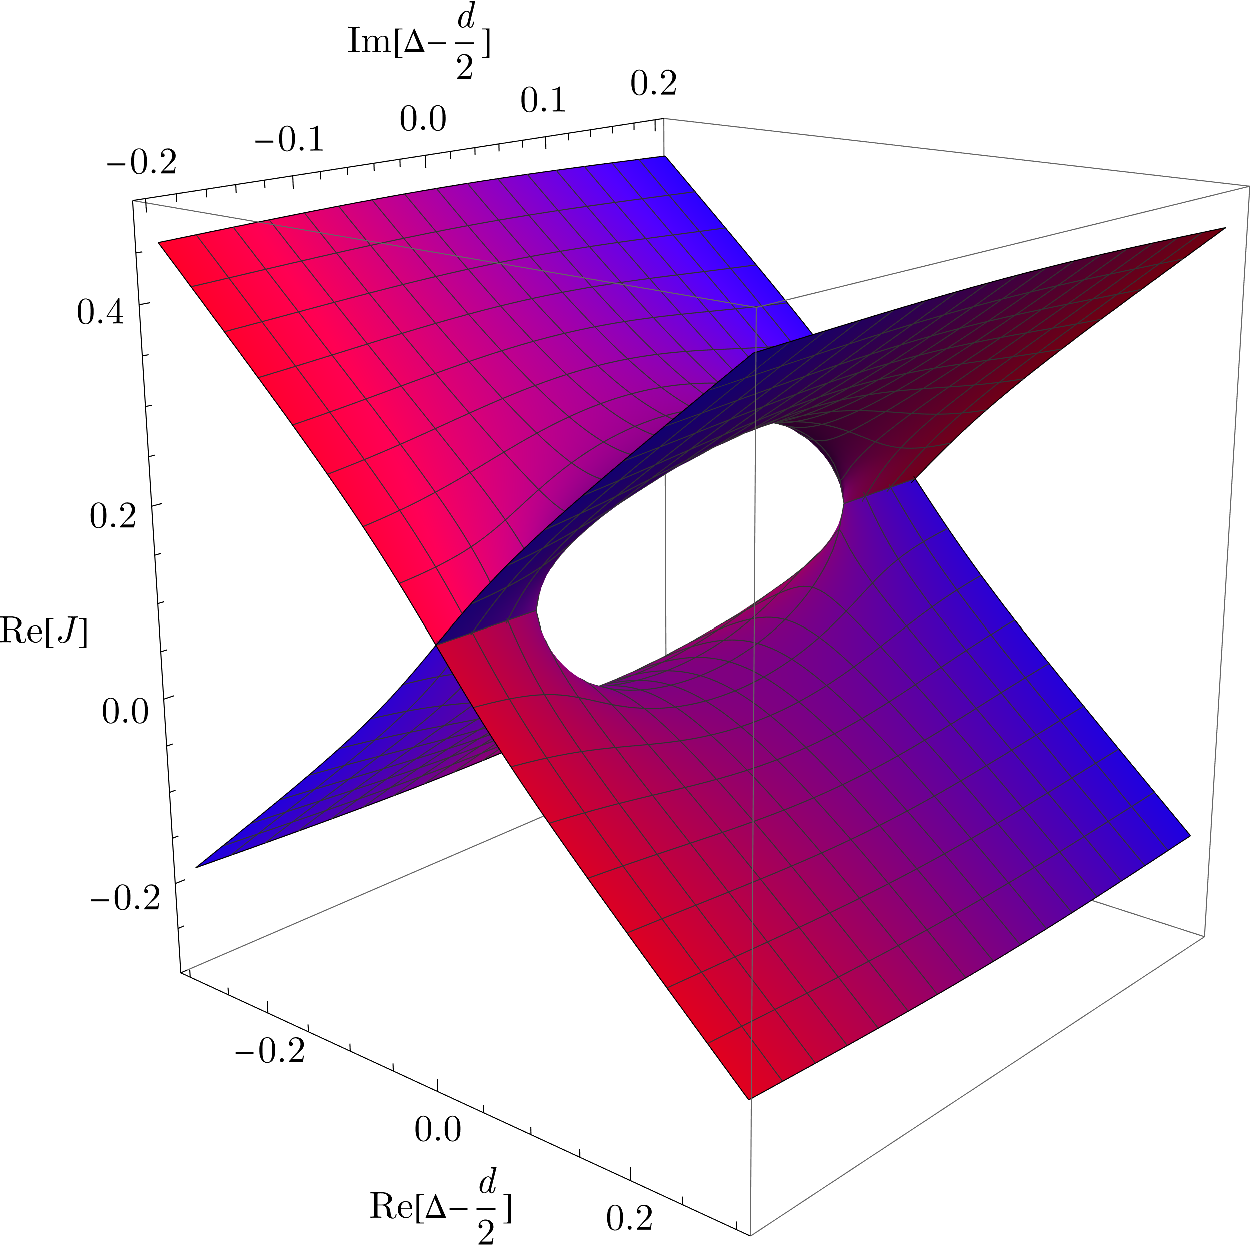
\includegraphics[scale=.5]{Figures/3dIntercept.pdf}
    \caption{The figure taken from \cite{Caron-Huot:2022eqs}. An $\mathbb{R}^3$ projection of the $\mathbb{C}^2$ Chew-Frautschi plot of the leading Regge trajectory in Wilson-Fisher theory near the intercept at $O(\e^4)$.  The imaginary part of $J$ is shown by color, with negative values in blue and positive values in red. Even though the two branches appear to intersect, they do not -- in order to intersect in $\mathbb{C}^2$, they need to intersect in this $\mathbb{R}^3$ projection and also have the same color.  The plot is made at $\e=0.3$.}
    \label{fig:3dintercept}
  \end{center}
\end{figure}

\begin{figure}[t!]
  \centering
  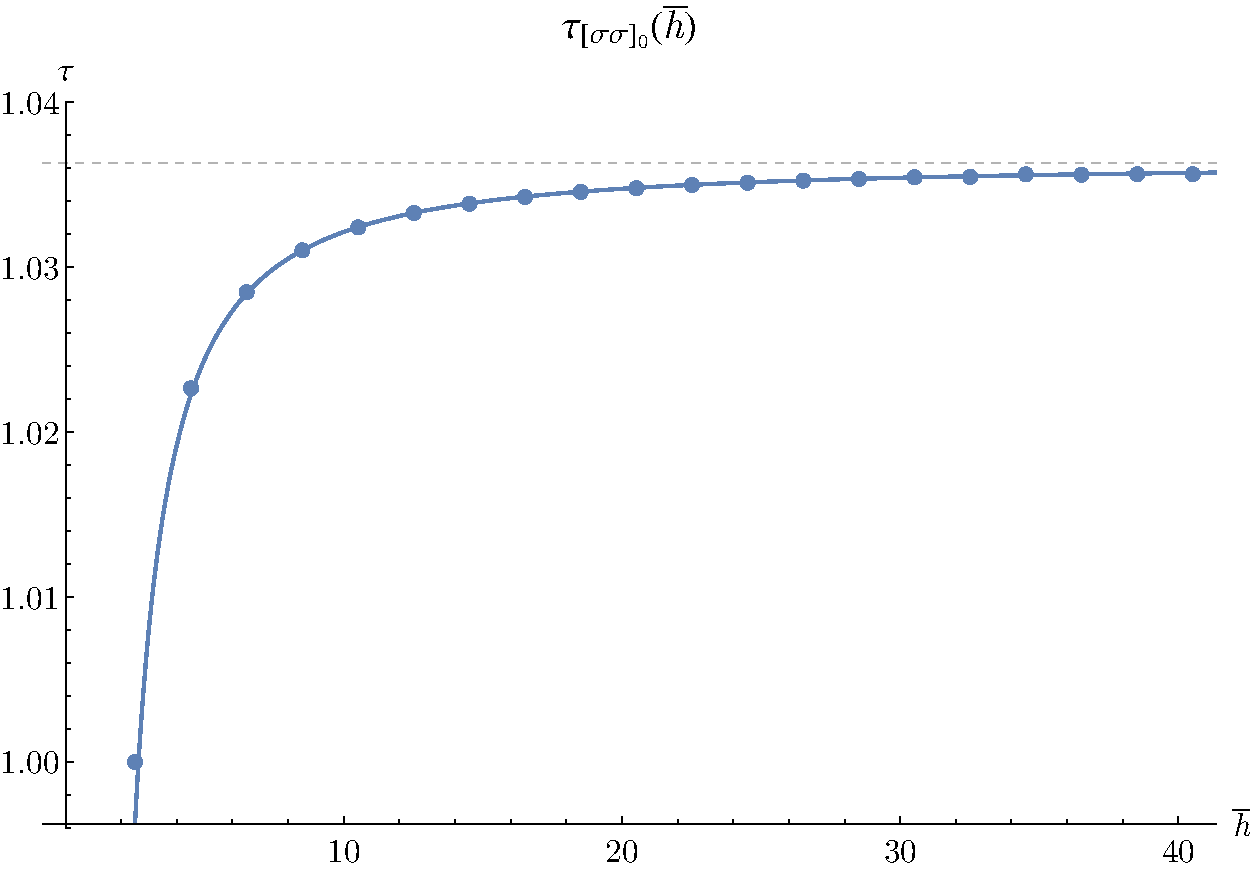
\includegraphics[width=0.8\textwidth]{Figures/tauSigSig0.pdf}
  \caption{Results from the numerical analysis \cite{Simmons-Duffin:2016wlq}.
    It depicts the spectrum of operators in the operator product expansion of $ \sigma \times \sigma $.
    To facilitate the comparison with analytic result, the vertical axis plots $  \tau= \Delta- J $, `twist' and $ \bar{h} = \frac{\Delta + J}{2} $.
    Notice the present of stress-tensor with $ \Delta = 3 , \tau = 1$.
    The continuous line is the extrapolation of the large spin perturbation theory around $ J = \infty $.
    While the spin $ J = \bar{h} - h  $ is as small as $ 2 $, we find a remarkable agreement with the numerics.
  }
  \label{fig:DSDLightcone}
\end{figure}
\section{Plan of the thesis}
The discussion of the analyticity in spin sets the stage for the thesis.
The goal of the thesis is to consider two aspects of Regge theory.
\subsection*{Optical theorem in AdS}
In recent years it has been shown that powerful analytical results for scattering amplitudes in quantum field theory, namely the Froissart-Gribov formula and dispersion relations, have equally powerful CFT analogues in the Lorentzian inversion formula \cite{Caron-Huot:2017vep,Karateev:2018oml,Kravchuk:2018htv,Lemos:2017vnx,Liendo:2019jpu} and the two-variable CFT dispersion relation \cite{Carmi:2019cub,Caron-Huot:2020adz}. Dispersion relations reconstruct a scattering amplitude from the discontinuity of the amplitude, while the Froissart-Gribov formula extracts the partial wave coefficients from the discontinuity and makes their analyticity in spin manifest. The utility of these methods as computational tools for scattering amplitudes stems from the fact that the discontinuity of an amplitude (or that of its integrand) in perturbation theory is determined in terms of lower-loop data by the optical theorem, which in turn is a direct consequence of unitarity.
The CFT analogue of the discontinuities of amplitudes, which contain the dispersive data and are of central importance in the aforementioned analytical results, is the double discontinuity (dDisc) of CFT four-point functions. The Lorentzian inversion formula
computes OPE data (anomalous dimensions and OPE coefficients) from the dDisc of four-point functions and establishes the analyticity in spin of OPE data. The CFT dispersion relation, much like its QFT inspiration, directly reconstructs the full correlator from the dDisc. There also exist simpler single-variable dispersion relations in terms of a single discontinuity (Disc) of the correlation function that determine only the OPE coefficients while the anomalous dimensions are required as inputs \cite{Bissi:2019kkx}.

The unitarity based methods to compute amplitudes  inspire the development of  similar unitarity methods for CFT, in particular,
for the dDisc of four-point functions one gains a loop or leg order for free.
It was first noticed in large spin expansions \cite{Alday:2016njk,Alday:2016jfr,Aharony:2016dwx} and later understood more generally in terms of the Lorentzian inversion formula
that OPE data at one-loop can be obtained from tree-level data \cite{Alday:2017vkk,Alday:2017zzv}. Generically, in perturbative CFT calculations the dDisc at a given order only depends on OPE data from lower order or lower-point correlators. More recently, in the context of the AdS/CFT correspondence \cite{Maldacena:1997re,Witten:1998qj,Gubser:1998bc},
these unitarity methods for CFT have been related to cutting rules for computing the dDisc of one-loop Witten diagrams \cite{Liu:2018jhs} from tree-level diagrams \cite{Ponomarev:2019ofr,Meltzer:2019nbs,Meltzer:2020qbr}.
See also the earlier work of \cite{Fitzpatrick:2011dm}.

However, so far we have been missing a direct adaptation of the optical theorem to CFT correlation functions.
More concretely, we lacked the ability to express the dDisc of a perturbative correlator, at a given order in the perturbative parameter, in terms of lower order correlators, without the detour via the OPE data and without making explicit reference to AdS Witten diagrams.
In the first chapter, we provide a direct CFT derivation of such unitarity relations.
In particular, we present an optical theorem for 1-loop four-point functions wherein the dDisc is fixed in terms of single discontinuities of lower-loop  correlators.

\subsection*{Conformal multi-Regge theory}

Constraints from the bootstrap analysis of the four point correlation functions are known to be powerful in obtaining remarkable accurate and precise physical data such as critical exponents of the theories appearing in the nature.
The main idea is that any function of two cross ratios can not  be a valid correlation function.

This suggests that there might be more constraints in the consistency of higher point correlation functions.
Since higher point functions can be decomposed into correlation functions with fewer number of points, these constraints are implicitly present in the four point bootstrap analysis.
However, we might need to explore \emph{infinitely} many four point functions to probe them.
For instance, a single five point correlation function can be decomposed into infinitely many four point functions.
This calls for a careful study of such high point functions.

In the third chapter, our goal is to initiate such a program.
The goal is to introduce a useful definition of Regge limit for five point correlation functions in conformal field theories.
First, we review the relevant literature from S-matrix theory.
In particular, we discuss the multi-Regge limit of five point string theory amplitudes.

Inspired by this analysis, we propose the generalization to the conformal field theory.
Since the natural analogue of the Mandelstam invariants is the Mellin space, we discuss this generalization mainly in Mellin space.
We also show its relation to position space and the corresponding spacetime structure.

Furthermore, we comment on the relation between the Reggeized correlator and the CFT data such as the OPE coefficients and the scaling dimensions of the operators on the leading Regge trajectory.
In passing, we also discuss several interesting kinematical aspects of higher point correlation functions.
We expect them to be useful in generalizing the discussion of the inversion formula and the dispersion relation to the higher point functions.

Now, we turn to the analysis of the optical theorem in $ AdS $.
\cleardoublepage

% % % Chapter Template

% \chapter{Conformal field theory and Regge limit} % Main chapter title
% \label{Conformal field theory and Regge limit}

% \section{Kinematics of conformal field theory}
% In this section, we discuss the kinematics of conformal field theory.
% Conformal field theories in $ d $ dimensions are a class of quantum field theories with additional symmetries that are not present in the standard quantum field theories.
% In the Euclidean space, the conformal field theories are invariant under the Euclidean conformal group, $ SO(d+1,1) $, while in the Lorentzian space they are invariant under the Lorentzian conformal group, $ SO(d,2) $.
% The generators of the Euclidean conformal group can be written in terms of the spacetime derivative $ \partial_{\mu} $.
% \begin{align}
% 	\text{Translations}                      &  & P_{\mu} & = \partial_{\mu}                                                             \\
% 	\text{Rotations}                         &  & M_{\mu} & =  i\left( x_\mu \partial_\nu - x_\nu \partial_\mu \right)                   \\
% 	\text{Dilatations}                       &  & D       & = i x^\nu \partial_\nu                                                       \\
% 	\text{Special conformal transformations} &  & K_{\mu} & = i\left( 2x_\mu \left( x^\nu \partial_\nu \right) -x^2 \partial_\mu \right)
% 	.
% \end{align}
% However, some of these generators act nonlinearly on the spacetime points.
% Therefore, it is useful to consider `Embedding space':
% \begin{align}
% 	X^A = \left( \frac{1+x^2}{2},\frac{1-x^2}{2},x^\mu  \right)  ,
% \end{align}
% with the signature $ \left( -,+,\dots,+ \right) $.
% The Euclidean conformal group acts linearly on $ X $.
% This simplifies several calculations, for instance, the inner product in the physical space $ \left( x_\mu -y_\mu \right) \left( x_\nu - y_\nu \right) \delta^{\mu\nu} $ becomes $ X\cdot Y =X_A Y_B \eta^{A B} $.
% Here, $ X,Y $ are respective embedding coordinates for $ x,y $.
% This allows us to identify the dependence on the spacetime variables of the correlations functions.

% The physical observables in conformal field theory are the correlation functions of the local operators in the theory.
% The local operators are characterized by quantum numbers of the generators of the conformal group.
% We consider a special set of operators, called `primary' operators.
% They are precisely the operators which are annihilated by special conformal transformations $ K_\mu O =0 $.
% All the other operators are `descendants' of one of these operators, namely, they are of the form: $ \left( P_\mu \right)^n O $.
% In particular, the operators are labeled by the quantum numbers for dilatations: $ \Delta $  and rotations: $ \lambda $, a Young tableux diagram for the representation.
% Thus, a representation of the conformal group $ R $ is labeled by $ \left( \Delta,\lambda \right) $.
% In the simple case of symmetric traceless representation, $ \lambda $ can be replaced by the number of boxes in $ \lambda $, representing the spin.

% Two and three points correlation functions of scalars, the operators with spin $ 0 $ and scaling dimensions $ \Delta_i $ can be written in terms of the embedding space as follows.
% \begin{align}
% 	\langle\phi\left( X \right) \phi\left( Y \right) \rangle                      & =\frac{\delta_{\Delta_1 \Delta_2}}{\left( X \cdot Y \right)^{\Delta_1}}                                                          \\
% 	\langle\phi\left( X \right) \phi\left( Y \right)\phi\left( Z \right)  \rangle & =\frac{c}{\left( X \cdot Y \right)^{\alpha_{123}}\left( Y \cdot Z \right)^{\alpha_{231}}\left( Z \cdot X \right)^{\alpha_{132}}}
% 	.
% \end{align}
% We have chosen the normalization of the operators such that the two point function numerators are $ 1 $.
% The numerator in the three point function, $ c $,  is called `operator product expansion coefficient' (OPE coefficient).
% We have also used $ \alpha_{ijk} = \left( \Delta_i + \Delta_j - \Delta_k \right)/2 $ .

% The set of representations $ R $'s of the local primary operators and their respective OPE coefficients $ c_{R_1,R_2, R_3} $ consitute a useful characterization of the observables in conformal field theory, called `\emph{CFT data}'.

% While it is easy to see that the spactime dependence of the two and three point functions are fully characterized by the conformal invariance, the situation changes for higher point functions.
% The four point function is not fixed by the conformal invariance because there exist conformal invariant `cross ratios'
% \begin{align}
% 	U=\frac{X_{12} X_{34}}{X_{13} X_{24}}, \,\, & V= \frac{X_{14}X_{23}}{X_{13}X_{24}}.
% 	\label{eq:crossRatios}
% \end{align}
% The dependence on these cross ratios can't be fixed by conformal invariance alone.
% This allows us to write the four point correlation function of identical scalars as
% \begin{align}
% 	\langle\phi\left( X_1 \right) \phi\left( X_2 \right)\phi\left( X_3 \right) \phi\left( X_4 \right) \rangle = \frac{1}{X_{12}^\Delta X_{34}^\Delta} A\left( U,V \right).
% \end{align}
% $ A $ denotes an unknown function of cross ratios.
% However, since the operators $ \phi $'s are identical, their correlation function is permutation invariant.
% It is easy to see that this leads to a constraint on $ A $, namely
% \begin{align}
% 	A\left( U,V \right) \left( \frac{V}{U} 	 \right)^\Delta & = A\left( V,U \right) .
% \end{align}
% This is called as the `\emph{crossing constraint}'

% The goal of conformal bootstrap is to use the consistency conditions of the conformal field theory to constrain the CFT data.
% In particular, we use consistency of the four point function to arrive at constraint on the lower point functions.

% In conformal field theories, one can use `\emph{operator product expansion}'.
% \begin{align}
% 	\phi\left( x \right) \phi\left( y \right) = \sum_{\textit{primary } O} c_{\phi \phi O}\left( x-y,\partial_{x-y} \right) O\left( y \right)	.
% \end{align}
% Unlike a generic quantum field theory, this expansion has a finite radius of convergence.
% This is an operator level statement and therefore is valid in all correlation functions.
% In particular, it can be used to write down a four point correlation function in terms of the lower point correlation function.
% \begin{align}
% 	\langle\phi\left( x \right) \phi \left( y \right)\times \phi \dots \phi \rangle &
% 	= \sum_{\textit{primary } O} c_{\phi \phi O}\left( x-y,\partial_{x-y} \right) \langle O\left( y \right) \phi \dots \phi\rangle	.
% \end{align}
% Note that the right hand side correlation function has fewer operator insertions than the left hand side correlation function.

% All quantum field theories are unitary.
% Unitarity of conformal field theory, which is also a conformal field theory imposes constraint on the CFT data.
% The OPE coefficient is a real number.
% This leads to a nontrivial constraint on the four point correlation function when expanded in terms of the lower point correlation functions.

% These constraints are used in the program of Euclidean conformal bootstrap.
% However, in this thesis, we are mainly concerned with the constraints coming from the Lorentzian consistency of the conformal field theory.
% In the following, we discuss the necessary tools to discuss correlation function in the Lorentzian setup and its relation to the Euclidean correlation function.

% % \todo[inline]{
% % 	Describe the conformal group and its action of the spacetime transformations.

% % 	representation theory

% % 	define primary descendants

% % 	Constraints from Unitarity mentioned above.
% % }

% % \section{Constraints on the correlation functions}
% % \todo[inline]{

% % 	Four points are not.

% % 	Crossing symmetry

% % 	Bootstrap comes from constraints from Unitarity along with crossing symmetry.
% % }


% % Definitions relevant for the Regge limit: Lightcones , dDisc


% \section{Wightman functions}
% In this section, we discuss the Wightman functions and their properties.
% The Wightman functions are useful in going back and forth between the properties of Lorentzian correlators and their Euclidean counterparts.

% % \todo[inline]{
% % 	Add discussion of Wightman functions etc
% % }
% For concreteness, we consider the correlation function of four identical scalars $ \phi $.
% First, we discuss the Euclidean correlation function in the Euclidean space with time direction denoted by $ \tau $ and space directions labelled by $ y_i $.
% As discussed before, such a correlation function is fixed up a function, $ A $, of two cross ratios $ U,V $.
% We define a rewriting of the cross ratios $ U  = z \bar{z}$ and $ V = \left( 1-z \right) \left( 1-\bar{z} \right) $.
% This rewriting is especially useful when we use the conformal symmetry to fix three out of the four points to be at $ 0,1,\infty $.
% The point that is not fixed can be brought to the same plane as the other three points by a conformal transformation.
% The location of this point is precisely $ z $ in the complex plane $i \tau + y $ .
% We choose the second point to be written in terms of $ z $.
% Thus, the Euclidean correlation function is given by $ A\left( z,\bar{z}=z^* \right) $.
% Note that in the Euclidean setup, we have $ \bar{z} = z^* $, since $ \tau $ is real.
% Now, we would like to discuss the procedure to convert this correlation function to a Lorentzian correlation function.
% In this case, the Euclidean time becomes purely imaginary.
% Therefore, $ z,\bar{z} $ are no longer complex conjugates of each other, but are in fact complex numbers with imaginary part being small.

% In the Lorentzian setup, commutator of two operators spacelike separated.
% \begin{align}
% 	\left[ O_1\left( x_1 \right),O_2\left( x_2 \right) \right] = 0 &  & x_1 \approx x_2.
% \end{align}
% In particular, if we move the point $ x_2 $ from the region spacelike separated from $ x_1 $ to the region timelike separated from $ x_1 $, the commutator encounters a jump.
% This jump is reminiscant of branch cut behaviour.
% In fact, the correlation function in the Lorentzian setup is given by an appropriate analytic continuation of the Euclidean correlation function.
% One expects that the function $ A $ admits a branch cut when two of the points in the correlation function become lightlike separated.

% We study the correlation function by first starting in the Euclidean setup with points fixed at
% \begin{align}
% 	x_1 & = \left( 0,0,\dots,0 \right) & x_2 & = \left( \tau_2,y_2,\dots,0 \right) \nonumber \\
% 	x_3 & = \left( 0,1,\dots,0 \right) & x_4 & = \left( 0,\infty,\dots,0 \right)
% 	.
% \end{align}
% Now, the idea is to move the second point away from the Euclidean space positions to Lorentzian space positions.
% This involves a Wick rotation $ \tau \rightarrow i t $ with appropriate $ i\epsilon $ prescription.
% While doing so, one can encounter a branch cut due to the presence of the lightcones in the Lorentzian spacetime.
% It is easy to see that the location of the branch cuts in $ \tau_2 $ is as depicted in figure \ref{fig:cutsInTau}.
% Going from Euclidean to Lorentzian, the value of $ \tau_2 $ goes from a real number to a purely imaginary number.

% One can study the implications of this branch cuts on the correlation function as a function of the cross ratios.
% This branch cuts implies a branch cut in the correlation function at $ z,\bar{z} \in \left( 1,\infty \right)  $.

% \begin{figure}[t]
% 	\centering
% 	\begin{tikzpicture}
% 		%name
% 		\draw[] (-5.2,3) -- (-5.2,2.5) -- (-5.7,2.5);
% 		\node[left] at (-5.2,2.8) {$\tau_2$};
% 		%axis
% 		\draw[->,opacity=0.3,-latex'] (0,0) -- (-5,0);
% 		\draw[->,opacity=0.3,-latex'] (0,0) -- (0,3);
% 		\draw[->,opacity=0.3,-latex'] (0,0) -- (0,-3);
% 		\draw[->,opacity=0.3,-latex'] (0,0) -- (5,0);
% 		%drawing points 
% 		\draw[fill=black] (0,1) circle (0.05);
% 		\draw[fill=black] (0,2) circle (0.05);
% 		\draw[fill=black] (0,-1) circle (0.05);
% 		\draw[fill=black] (0,-2) circle (0.05);
% 		%labelling
% 		\node[left] at (-0.4,1) {$i(y_2-y_1)$};
% 		\node[right] at (0,2) {$i(y_3-y_2)$};

% 		\node[left] at (0,-2) {$-i(y_3-y_2)$};
% 		\node[left] at (0,-1) {$-i(y_2-y_1)$};
% 		%drawing cuts
% 		\draw[red,opacity=0.8,dashed] (0,1) -- (-0.3,3);
% 		\draw[red,opacity=0.8,dashed] (0,2) -- (-0.3,4);

% 		\draw[red,opacity=0.8,dashed] (0,-2) -- (0.3,-4);
% 		\draw[red,opacity=0.8,dashed] (0,-1) -- (0.3,-3);
% 		\draw[black,opacity=0.8] (3,0) -- (-0.3,0.5);
% 		\draw[black,opacity=0.8] (3,0) -- (0,2) -- (-0.3,0.5);
% 	\end{tikzpicture}
% 	\caption{Location of cuts in the complex $\tau$ plane.
% 		The grey lines are the possible path, with or without crossing the branch cuts.}
% 	\label{fig:cutsInTau}
% \end{figure}

% This exotic branch structure allows us to probe more constraints on the correlation function.
% In particular, there are constraints coming from the Lorentzian consistency which are hard to see from the Euclidean CFT understanding.
% Euclidean correlation functions are simplified in the `OPE limit', when two of the points are colliding.
% This is a somewhat singular limit, but allows us to study the correlation function analytically.
% This corresponds to $ z \rightarrow 0,1 \text{ or }  \infty $ limit in the correlation function $ A $.
% The complicated structure of cuts allows us access to a bigger set of singular structure of the correlation function.
% We can choose to cross some of these branch cuts \emph{before} taking the limit $ z \rightarrow 0,1 \text{ or }  \infty $.
% Study of such limits of the correlation function is called `Regge theory'.

% % \subsection{Chaos bound}
% % Implications such as Regge boundedness and chaos bound.
% \section{Regge theory}
% We discuss some aspects of Regge theory in this section.
% Regge theory concerns the study of the correlation function in the `Regge limit'.
% This is a generalization of the `Regge limit' in the scattering amplitudes, which concerns the high energy limit.

% Consider the case of two to two scattering amplitudes.
% They are described in terms of the momenta of the external particles, $p_1, p_2, p_3, p_4$.
% However, due to conservation of momenta as well as Lorentz invariance of the theory, they depend only on the two invariants, $s = \left( p_1 + p_2 \right)^2$ and $ t = \left( p_1 + p_3 \right)^2 $.
% Regge limit concerns an extreme high energy scattering limit wherein $ s $ is large while $ t $ is fixed.

% Analogously, the correlation functions of four operators in a Lorentzian conformal field theory depend on two cross ratios, $ U,V $, defined in equation \ref{eq:crossRatios}.
% In terms of these cross ratios, one can consider various limits.
% One can consider the `OPE limit' where two of the four operators approach each other.
% This amounts to $ U \rightarrow 0, V \rightarrow 1 $ with $ \left( V-1 \right)/\sqrt{U} $ fixed.
% The latter, $ \xi $, is the analogue of the scattering angle in the S-matrix case.
% One can also consider the limit where one of the operators approach the lightcone of the other.
% This is called the `lightcone limit'.
% This amounts to $ U\rightarrow 0 $ for any $ V $.

% In the Regge limit, we are concerned with a certain generalization of the OPE limit.
% As described in the previous section, the correlation function has interesting analytic structure.
% Therefore, one has a lot more freedom to consider the generalization of the lightcone limit.
% Several lightcones of the form $ x_{ij}^2 = 0 $ are related to nontrivial analytic structure such as branch points and branch cuts in terms of the cross ratio space $ U,V $.
% Regge limit concerns the OPE limit, however, it is taken after crossing the cuts in $ V $ cross ratio at $ V = 1 $.

% In the following, we study the effect of this limit on the correlation function of four operators, $ \phi $.
% Using conformal symmetry, we first represent the correlation function in terms of the cross ratios, $ A\left( U,V \right) $.
% It admits an expansion in terms of certain kinematical functions of cross ratios called `conformal blocks', denoted by $ G $.
% \begin{align}
% 	A\left( U,V \right) & = \displaystyle\sum_{O} \lambda_{\phi \phi O}^2 G_{O}\left( U,V \right).
% \end{align}
% These objects are defined for each primary $ O $ and come from summing over all the descendants of a given primary $ O $.
% Each primary is a representation of the Euclidean conformal group, and therefore labeled by scaling dimensions, $ \Delta $ and the representation of the rotation group, $ \Lambda $.
% For the symmetric traceless representation of the rotation group, it is just the spin quantum number.
% While these are interesting objects themselves, it is useful to rewrite the expansion in terms of `conformal partial waves', $ F_{O} $.
% Similar to the S-matrix partial waves, these partial waves have a well defined orthogonality properties.
% They can be expressed as a linear combination of the conformal block as follows.
% \begin{align}
% 	F_{O} = G_O + \frac{\kappa_{\tilde{O} }}{ \kappa_{O}} G_{\tilde{O}}
% 	.\end{align}
% The orthogonality holds for the operators on the `principle series representations'.
% These are operators whose scaling dimensions is $ d/2 + i \mathbb{R} $.
% orthogonality relation can be written in terms of some weight function $ w $ as
% \begin{align}
% 	\int dU dV \, w\left( U,V \right) F_{O}\left(U,V \right) F_{O'}\left(U,V \right) = n_{O} \delta_{O \, O'}
% 	.
% \end{align}

% Now, we consider the Regge limit of the partial wave expansion in the spacetime dimensions $ d = 2 h $.
% \begin{align}
% 	A\left( U,V \right) & = \displaystyle\sum_{J} \displaystyle\int_{h+ i \mathbb{R}}
% 	\frac{
% 		d\nu}{2\pi i }
% 	b_{\nu,J} F_{\nu,J}\left( U,V \right),                                                    \\
% 	b_{\nu,J}           & =\frac{ \lambda_{\phi \phi O}^2}{\nu^2 - \left( \Delta-h \right)^2}
% 	.
% \end{align}
% Here, we have introduced the `OPE function' $ b_{\nu,J} $.
% It is an analytic function of $ \nu $ with poles at the location of the physical operators.

% We discuss the analytic structure of the correlation function in the Regge limit as a function of $ V $.
% The lightcones result in two branch point singularities at $ V = 1 $ and $ V= \infty $.
% To separate them, we write a decomposition of the correlator as follows
% \begin{align}
% 	A & =
% 	A_+ +
% 	A_-
% 	,\end{align}
% such that the first one has no nontrivial monodromy around $ V =1  $, whereas the later has no nontrivial monodromy around $ V= \infty $.
% Corresponding to each, we define the `signatured OPE function'.
% They are the coefficient of the partial wave expansion of the signatured correlator.
% \begin{align}
% 	A^{\theta }\left( U,V \right) & = \displaystyle\sum_{J} \displaystyle\int_{h+ i \mathbb{R}}
% 	\frac{
% 		d\nu}{2\pi i }
% 	b_{\nu,J}^{\theta} F_{\nu,J}\left( U,V \right)
% 	.
% \end{align}
% They get contributions from even and odd spins, respectively.
% It is now known that these `signatured OPE functions' are also analytic functions of $ J $ \cite{Caron-Huot:2017vep}.
% Thus, even and odd spins form `Regge trajectories'.
% These are interesting analytic manifolds with analyticity in $ J $.

% First, we discuss the limiting behaviour of the conformal partial wave in the Regge limit. 
% This limit can be written as $ \sigma \rightarrow 0 $ with fixed $ \xi  $ where we use
% \begin{align}
% 	\sigma^2 = z \bar{z}, \,  && \xi =\frac{1}{2} \left(
% \sqrt{\frac{z}{\bar{z}}} + \sqrt{\frac{\bar{z}}{z}}
% 	  \right) 
% .\end{align}
% As we will discuss later in the thesis, the Regge limit of the partial wave in generic dimensions is $ \sigma^{1-J}  $.
% Thus, the leading contribution to the correlator comes from the operators with higher spins.
% However, operators with arbitrarily large spin appear in the spectrum. 
% To make sense of this sum over spins, we use the techniques from complex analysis.


% We will use the analyticity in spin in the following.
% We discuss the evaluation of the correlator in the Regge limit described above.
% First, we replace the sum over spins by a contour integral over the positive real line, shown in blue in \cref{fig:polesInJ}.
% Then, we consider deforming this contour to the red contour.
% In the process, we pick any pole that we may encounter.
% This pole is called `the pomeron'.
% Thus, the leading behaviour of the correlator in the Regge limit is given by 
% \begin{align}
% \sigma^{1-j^{*}}
% ,\end{align}
% where $ j^{*} $ is the location of the circled pole in \cref{fig:polesInJ}.


% \begin{figure}[ht!]
% 	\centering
% 	\begin{tikzpicture}
% 		%name
% 		\draw[] (-1.2,3) -- (-1.2,2.5) -- (-1.7,2.5);
% 		\node[left] at (-1.2,2.8) {$J$};
% 		%axis
% 		\draw[->,opacity=0.3,-latex'] (0,0) -- (-1.5,0);
% 		\draw[->,opacity=0.3,-latex'] (0,0) -- (0,3);
% 		\draw[->,opacity=0.3,-latex'] (0,0) -- (0,-3);
% 		\draw[->,opacity=0.3,-latex'] (0,0) -- (5.8,0);
% 		%drawing points 
% 		\draw[fill=black] (0,0) circle (0.05);
% 		\draw[fill=black] (1,0) circle (0.05);
% 		\draw[fill=black] (2,0) circle (0.05);
% 		\draw[fill=black] (3,0) circle (0.05);
% 		\draw[fill=black] (4,0) circle (0.05);
% 		\draw[fill=black] (5,0) circle (0.05);
% 		\draw[fill=black] (0.3,1) circle (0.05);

% 		% \draw[] (-0.662,0.830591) -- (-0.331,1.16178);
% 		% \draw[] (-0.822,0.771524) -- (-0.272,1.32161);
% 		% \draw[] (-0.9416,0.752275) -- (-0.252,1.44162);
% 		% \draw[] (-1.0434,0.751257) -- (-0.251,1.5434);
% 		% \draw[] (-1.133,0.761969) -- (-0.262,1.63345);
% 		% \draw[] (-1.215,0.78141) -- (-0.281,1.71478);
% 		% \draw[] (-1.289,0.807926) -- (-0.308,1.78902);
% 		% \draw[] (-1.357,0.84052) -- (-0.341,1.85719);
% 		% \draw[] (-1.420,0.878568) -- (-0.379,1.91991);
% 		% \draw[] (-1.478,0.921687) -- (-0.422,1.97755);
% 		% \draw[] (-1.530,0.96967) -- (-0.470,2.03033);
% 		% \draw[] (-1.578,1.02245) -- (-0.522,2.07831);
% 		% \draw[] (-1.621,1.08009) -- (-0.580,2.12143);
% 		% \draw[] (-1.659,1.14281) -- (-0.643,2.15948);
% 		% \draw[] (-1.692,1.21098) -- (-0.711,2.19207);
% 		% \draw[] (-1.719,1.28522) -- (-0.785,2.21859);
% 		% \draw[] (-1.738,1.36655) -- (-0.867,2.23803);
% 		% \draw[] (-1.749,1.4566) -- (-0.9566,2.24874);
% 		% \draw[] (-1.748,1.55838) -- (-1.0584,2.24772);
% 		% \draw[] (-1.728,1.67839) -- (-1.178,2.22848);
% 		% \draw[] (-1.669,1.83822) -- (-1.338,2.16941);
% 		%drawing circles
% 		\draw[<-,line width=0.7,blue] (0.2,0) to[out=90,in=0] (0,0.2) to[out=180,in=90] (-0.2,0) to[out=-90,in=180] (0,-0.2) to[out=0,in=-90] (0.2,0);
% 		\draw[<-,line width=0.7,blue] (1.2,0) to[out=90,in=0] (1,0.2) to[out=180,in=90] (0.8,0) to[out=-90,in=180] (1,-0.2) to[out=0,in=-90] (1.2,0);
% 		\draw[<-,line width=0.7,blue] (2.2,0) to[out=90,in=0] (2,0.2) to[out=180,in=90] (1.8,0) to[out=-90,in=180] (2,-0.2) to[out=0,in=-90] (2.2,0);
% 		\draw[<-,line width=0.7,blue] (3.2,0) to[out=90,in=0] (3,0.2) to[out=180,in=90] (2.8,0) to[out=-90,in=180] (3,-0.2) to[out=0,in=-90] (3.2,0);
% 		\draw[<-,line width=0.7,blue] (4.2,0) to[out=90,in=0] (4,0.2) to[out=180,in=90] (3.8,0) to[out=-90,in=180] (4,-0.2) to[out=0,in=-90] (4.2,0);
% 		\draw[<-,line width=0.7,blue] (5.2,0) to[out=90,in=0] (5,0.2) to[out=180,in=90] (4.8,0) to[out=-90,in=180] (5,-0.2) to[out=0,in=-90] (5.2,0);

% 		\node[below] at (0.2,-0.1) {$0$};
% 		\node[below] at (1.2,-0.1) {$1$};
% 		\node[below] at (2.2,-0.1) {$2$};
% 		\node[below] at (3.2,-0.1) {$3$};
% 		\node[below] at (4.2,-0.1) {$4$};
% 		\node[below] at (5.2,-0.1) {$5$};
% 		%main contour before deforming
% 		\draw[->,line width=0.7,red] (0.5,1) to[out=90,in=0] (0.3,1.2) to[out=180,in=90] (0.1,1) to[out=-90,in=180] (0.3,0.8) to[out=0,in=-90] (0.5,1);
% 		\draw[->,line width=0.7,red,-latex'] (-1,-3) -- (-1,3);

% 		\node[above right] at (0.3,1.1) {$j(\nu)$};
% 	\end{tikzpicture}
% 	\caption{Location of poles in the complex $ J$ plane.}
% 	\label{fig:polesInJ}
% \end{figure}

% This sets the stage for the rest of the thesis concerning the applications of the Regge theory.
% Now, we turn to the application of these ideas to optical theorem in AdS.
% \cleardoublepage

%  \part{Optical theorem in AdS}

\chapter{Optical theorem in AdS}
\label{part:opticalTheoremPaper}

% Chapter Template

% \chapter{Optical theorem} % Main chapter title
% \label{Optical theorem}

% Write text in here
% Use \subsection and \subsubsection to organize text


\section{Introduction}
\label{sec:intro}


Let us briefly describe the logic that underlies the perturbative CFT optical theorem. Throughout this chapter we will  consider the  correlator
\beq
A(y_i) = \< \cO_1 (y_1) \cO_2 (y_2) \cO_3 (y_3) \cO_4 (y_4)  \>\,.
\eeq
We begin by expanding the dDisc of this correlator in $t$-channel  conformal blocks.
We may do this by expanding in conformal partial waves and then projecting out the contribution of the
exchange  of the shadow operator $\tilde{\cO}$. The advantage of this procedure is that  when
writing the partial waves as an integrated  product of three-points functions, the dDisc operation factorizes as a product of discontinuities,
\beq
\dDisc_t A(y_i) =
-\frac{1}{2}
\sum\limits_{\cO} \int dy dy' \,
\Disc_{23} \< \cO_2 \cO_3  \cO (y) \>  \<\tilde{\cO} (y) \tilde{\cO} (y') \>  \Disc_{14}  \< \cO_1 \cO_4  \cO (y') \>
\Big|_{\cO}\,,
\label{eq:general_contribution}
\eeq
where we use the shorthand notation $d^dy\equiv dy$.
Notice that the sum runs over all operators in the theory.
We give the precise definitions of the double and single discontinuities of the correlator in section \ref{sec:glue}.

Next, let us assume  that the correlator admits an expansion in a small parameter around mean field theory (MFT).
The example we have in mind is the
$1/N^2$ expansion,
\beq
A = A_\text{MFT} + \frac{1}{N^2} A_\text{tree} + \frac{1}{N^4} A_\text{1-loop} + \cdots \,.
\label{eq:loop_expansion}
\eeq
We can then separate the sum over intermediate operators $\mathcal{O}$ into single-, double-, and higher-trace operators, and rewrite the multi-trace contributions as
higher-point functions of single-trace operators.
The contribution of single-trace operators to the $t$-channel expansion of dDisc
in \eqref{eq:general_contribution} is left unchanged and is still given
in terms of discontinuities of three-point functions
\bea
\dDisc_t A(y_i)\Big|_\text{s.t.} =
-\frac{1}{2}
\sum\limits_{\cO \in s.t.} \int dy dy' \,
\Disc_{23} \< \cO_2 \cO_3  \cO (y) \> \<\tilde{\cO} (y) \tilde{\cO} (y') \>   \Disc_{14}  \< \cO_1 \cO_4  \cO (y') \>
\Big|_{\cO}\,.
\label{eq:stcontribution}\end{aligned}\end{equation}
Here no simplifications occur, however this contribution is already simple as
loop corrections come from corrections to the three-point functions of single-trace operators.

The essential simplification that we call the perturbative optical theorem arises for the
contributions of double-trace operators to \eqref{eq:general_contribution}, which are now expressed in terms of
discontinuities of four-point functions of single-trace operators
\begin{align}
\dDisc_t A_{\rm 1-loop}(y_i)\Big|_\text{d.t.} \!
= -\frac{1}{2}
\sum\limits_{\substack{\mathcal{O}_5,\mathcal{O}_6\\ \in\  s.t.}}
\!
\int dy_5 dy_6 \, \Disc_{23}  A_{\rm tree}^{3652}(y_k) \; \bS_{5}\bS_{6}\Disc_{14} A_{\rm tree}^{1564}(y_k)  \Big|_{[\cO_5 \cO_6]}\,.
\label{eq:cft_optical_theorem_intro}
.\end{align}

Here and henceforth, we shall use the notation $A^{abcd}(y_k)=\< \cO_a \cO_b  \cO_c \cO_d \>$
to denote the correlator of a set of operators other than $\< \cO_1 \cO_2  \cO_3 \cO_4 \>$, which we denote simply as $A(y_i)$.
$\bS_{5}\bS_{6} A^{1564}$ is defined as the shadow transform of $A^{1564}$ with respect to
the operators $\cO_{5}$ and $\cO_{6}$.
The operators $\cO_5$ and $\cO_6$ are summed over all single-trace operators for which the tree-level correlators exist. These may have spin, in which case the indices are contracted between the two tree-level correlators.
Importantly, in this case dDisc is of order $1/N^4$ and can be computed from the product of
the discontinuities of tree-level four-point functions, each of order  $1/N^2$.

Together equations (\ref{eq:stcontribution}) and (\ref{eq:cft_optical_theorem_intro})
compute the full double discontinuity at one-loop in large $N$ CFTs, since the contributions from higher traces will start at higher loops.
Their analogue is of course the optical theorem for amplitudes which computes discontinuities of one-loop amplitudes in terms of two- and one-line cuts. Note that although we use the notation
$A_\text{tree}$ and $A_\text{1-loop}$, these refer to conformal correlation functions and in general are not Witten diagrams. The notation with the terms ``one-loop" and ``tree" for the correlators is used only because we always refer to a perturbative expansion. The result is valid for CFTs with an expansion in a small parameter around MFT. The fact that it naturally handles cuts of spinning particles gives an advantage over previous CFT unitarity methods that work in terms of OPE data.

\begin{figure}
    \begin{equation*}
        \dDisc_t \,
        \diagramEnvelope{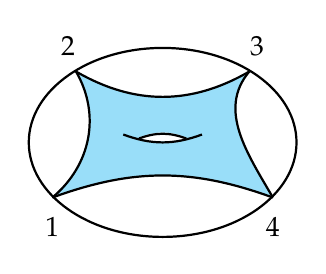
\begin{tikzpicture}[anchor=base,baseline]
                \node [coordinate] (BL) at (-1.4,-.7) {};
                \node [coordinate] (TL) at (-1.1, .9) {};
                \node [coordinate] (BR) at ( 1.4,-.7) {};
                \node [coordinate] (TR) at ( 1.1, .9) {};
                \node at (-1.4,-1.2) {$1$};
                \node at (-1.2, 1.1) [] {$2$};
                \node at ( 1.4,-1.2) [] {$4$};
                \node at ( 1.2, 1.1) [] {$3$};
                \draw [thick] (0,0) ellipse (1.7 and 1.2);
                \fill[cyan,fill opacity=0.4] (BR) to [out=160,in=20] (BL)
                to [out=40,in=300] (TL)
                to [out=330,in=210] (TR)
                to [out=230,in=120] cycle;
                \draw [thick] (BR) to [out=160,in=20] (BL);
                \draw [thick] (BL) to [out=40,in=300] (TL);
                \draw [thick] (TL) to [out=330,in=210] (TR);
                \draw [thick] (TR) to [out=230,in=120] (BR);
                \fill[white] (-.28,.07) to [out=20,in=160] (.28,.07)
                to [out=340,in=200] cycle;
                \draw [thick] (-.3,.05) to [out=20,in=160] (.3,.05);
                \draw [thick] (-.5,.1) to [out=340,in=200] (.5,.1);
            \end{tikzpicture}} \,
        \sim \sum\limits_{\cO_5, \cO_6} \int dy_{5,6}
        \Disc_{23}
        \diagramEnvelope{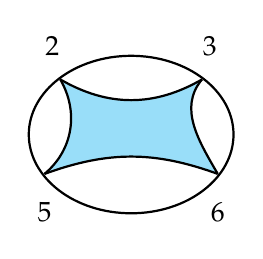
\begin{tikzpicture}[anchor=base,baseline]
                \node [coordinate] (BL) at (-1.1,-.5) {};
                \node [coordinate] (TL) at (-.9, .7) {};
                \node [coordinate] (BR) at ( 1.1,-.5) {};
                \node [coordinate] (TR) at ( .9, .7) {};
                \node at (-1.1,-1.1) {$5$};
                \node at (-1., 1.) [] {$2$};
                \node at ( 1.1,-1.1) [] {$6$};
                \node at ( 1., 1.) [] {$3$};
                \draw [thick] (0,0) ellipse (1.3 and 1.);
                \fill[cyan,fill opacity=0.4] (BR) to [out=160,in=20] (BL)
                to [out=40,in=300] (TL)
                to [out=330,in=210] (TR)
                to [out=230,in=120] cycle;
                \draw [thick] (BR) to [out=160,in=20] (BL);
                \draw [thick] (BL) to [out=40,in=300] (TL);
                \draw [thick] (TL) to [out=330,in=210] (TR);
                \draw [thick] (TR) to [out=230,in=120] (BR);
            \end{tikzpicture}}
        \Disc_{14}
        \diagramEnvelope{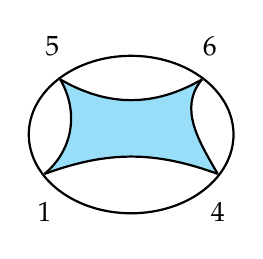
\begin{tikzpicture}[anchor=base,baseline]
                \node [coordinate] (BL) at (-1.1,-.5) {};
                \node [coordinate] (TL) at (-.9, .7) {};
                \node [coordinate] (BR) at ( 1.1,-.5) {};
                \node [coordinate] (TR) at ( .9, .7) {};
                \node at (-1.1,-1.1) {$1$};
                \node at (-1., 1.) [] {$\tl 5$};
                \node at ( 1.1,-1.1) [] {$4$};
                \node at ( 1., 1.) [] {$\tl 6$};
                \draw [thick] (0,0) ellipse (1.3 and 1.);
                \fill[cyan,fill opacity=0.4] (BR) to [out=160,in=20] (BL)
                to [out=40,in=300] (TL)
                to [out=330,in=210] (TR)
                to [out=230,in=120] cycle;
                \draw [thick] (BR) to [out=160,in=20] (BL);
                \draw [thick] (BL) to [out=40,in=300] (TL);
                \draw [thick] (TL) to [out=330,in=210] (TR);
                \draw [thick] (TR) to [out=230,in=120] (BR);
            \end{tikzpicture}}
    \end{equation*}
    \caption{In the Regge limit the dDisc of the genus one closed string amplitude in AdS is given by the perturbative CFT optical theorem in terms of genus zero amplitudes.}
    \label{fig:optical_theorem_string_pictures}
\end{figure}
In the second part of the chapter, we employ the perturbative CFT optical theorem in the context of the AdS/CFT correspondence \cite{Maldacena:1997re,Witten:1998qj,Gubser:1998bc}
to study high-energy scattering of strings in AdS, which is governed by the CFT Regge limit \cite{Cornalba:2006xk,Cornalba:2006xm}. This is illustrated in figure \ref{fig:optical_theorem_string_pictures}.
High-energy string scattering in flat space has been of interest for a long time, both in the fixed angle case \cite{Gross:1987kza,Gross:1987ar} and in the fixed momentum transfer Regge regime \cite{Amati:1987wq,Amati:1987uf,Amati:1988tn}. This second set of works studied the effects of the finite string size on the exponentiation of the phase shift (eikonalization) in the Regge limit. In particular,
it was shown that the amplitudes indeed eikonalize provided we allow the phase shift to become an operator acting on the string Hilbert space, whose matrix elements account for the possibility of the external particles becoming intermediate excited string states, known as tidal excitations.
The phase shift $\de(s,b)$, which depends on the Mandelstam $s$ and on the impact parameter $b$, is
obtained by Fourier transforming the amplitude with respect to momentum transfer
in the directions transverse to the scattering plane. This gives a multiplicative optical theorem of the form
\bea
\Im \de_{\text{1-loop}}(s,b)
={}& \frac{1}{2} \sum\limits_{\substack{m_5,\rho_5,\e_5\\m_6,\rho_6,\e_6}}
\de_\text{tree}^{3652}(s,-b)^* \,\de_\text{tree}^{1564}(s,b)\,,
\label{eq:impact_optical_theorem_flat}\end{aligned}\end{equation}
where the sum is over all possible exchanged particles, characterized by their mass $m_i$ and Little group representation $\rho_i$,
and their polarization tensors $\epsilon_i$.
In \cite{Amati:1987uf} the one-loop amplitude for four-graviton scattering in type IIB string theory was presented in a particularly nice form, where the tidal excitations, which constitute a complicated sum in \eqref{eq:impact_optical_theorem_flat}, are packaged into a single explicit scalar function, the so-called vertex function.

To study the analogous process in AdS we derive an AdS/CFT analogue of \eqref{eq:impact_optical_theorem_flat} by transforming the correlators in the CFT optical theorem \eqref{eq:cft_optical_theorem_intro} to AdS impact parameter space \cite{Cornalba:2006xk,Cornalba:2006xm}. This gives the following multiplicative optical theorem for CFTs
\beq
-\Re \cB_{\text{1-loop}}(p,\bar{p})  \Big|_{\text{d.t.}} = \frac{1}{2}
\sum\limits_{\cO_5, \cO_6 \in s.t.}
\cB^{3652}_\text{tree}(-\pb,-p)^*  \, \cB^{1564}_\text{tree}(p,\pb)  \Big|_{[\cO_5 \cO_6]} \,.
\label{eq:gluing_stripped_intro}
\eeq
Here $\cB$ denotes the impact parameter transform of $A$.
These transforms depend on two cross ratios $S$ and $L$, respectively interpreted as the square of the energy
and as the impact parameter of the AdS scattering process,
that can be expressed in terms of two $d$-dimensional vectors $p$ and $\bar{p}$, as will be detailed below.
When ${\cO_5}$ or ${\cO_6}$ have spin,  $\cB$ has tensor structures that depend on
$p$ and $\bar{p}$.
Equations \eqref{eq:gluing_stripped_intro} and \eqref{eq:impact_optical_theorem_flat} are related through the flat space limit for the impact parameter representation, where the radius of AdS is sent to infinity and where $\cB(p,\bar{p})$ is mapped to $i \de(s,b)$.
In this way, each of the infinite number of tree-level correlators with spinning particles 5 and 6 that appear on the right hand side of \eqref{eq:gluing_stripped_intro} is partially fixed by the corresponding flat space phase shift. Moreover, we will be able to efficiently describe the summed result in terms of an AdS vertex function,
which is in turn constrained by the one-loop flat space vertex function, as constructed for example for type IIB strings in  \cite{Amati:1987uf}.

For neutral scalar operators of dimension four in $d=4$, the four-point function considered here is dual to the scattering of four dilatons in the bulk of AdS$_5$. There are two expansion parameters that we need to consider, the loop order parameter $1/N^2$, and the 't Hooft coupling $\lambda$.
The large $\lambda$ limit is given by supergravity in AdS.
In this limit the tree-level four-point function is dominated by graviton exchange \cite{Cornalba:2006xk,Cornalba:2006xm} and beyond tree-level one can safely resum  the $1/N$ expansion by exponentiating the single graviton exchange \cite{Cornalba:2007zb,Brower:2007qh}.
For finite $\lambda$, string effects are included at tree-level via Pomeron exchange \cite{Brower:2006ea} and can
be described using conformal Regge theory \cite{Cornalba:2007fs,Costa:2012cb}.
A very non-trivial question we address in this chapter is the inclusion of string effects beyond tree-level.

To account for such effects in the Regge limit,
the earlier works  \cite{Cornalba:2007fs,Cornalba:2008qf,Brower:2007xg}
conjectured the exponentiation of the tree-level Pomeron  phase shift, assuming stringy tidal excitations to be negligible \cite{Cornalba:2009ax}.
More recently \cite{Meltzer:2019pyl}, the loop effects of Pomeron exchange were systematically taken into account from the CFT side in the AdS high-energy limit $S \gg \lambda \gg 1 $, with the crucial use of CFT unitarity to obtain higher-loop amplitudes from the lower-loop ones. This work also pointed out the suppression of tidal excitations in the supergravity limit $\lambda \gg 1$, in agreement with \cite{Cornalba:2007fs,Cornalba:2008qf,Brower:2007xg}. In the present work, we take finite $\lambda$ (or $\alpha'$) and include all tidal or stringy corrections. This is made possible because the perturbative CFT optical theorem is able to describe cuts involving spinning operators, so we can take into account
intermediate massive string excitations that are exchanged in the t-channel.

This chapter has the following structure. In section \ref{sec:glue}  we first motivate how \eqref{eq:general_contribution} for double-trace operators leads  to the perturbative CFT optical theorem \eqref{eq:cft_optical_theorem_intro} using the technique of ``conglomeration" \cite{Fitzpatrick:2011dm}, and then give a detailed derivation of \eqref{eq:cft_optical_theorem_intro} using tools from  harmonic analysis of the conformal group. Then in section \ref{sec:flat_space}
we review some important ideas from flat space scattering, including impact parameter space, unitarity cuts and the vertex function, both to guide the AdS version and to serve as a target for the flat space limit. We subsequently move to the holographic case in section \ref{sec:ads}, where we transform the correlator to CFT impact parameter space to write a multiplicative optical theorem for phase shifts.
We use conformal Regge theory in the case of arbitrary spinning operators leading to the derivation of the AdS vertex function. In section \ref{sec:Appendix_tchannel} we recover the results for the one-loop correlator in the large $\lambda$ limit \cite{Meltzer:2019pyl} and also derive new t-channel constraints on CFT data at finite $\lambda$. We give the details of the flat space limit prescription in section \ref{sec:flat_space_limit}, and consider the specific four-dilaton amplitude of type IIB strings in section \ref{sec:IIB_AdS_flat}, constraining  several spinning tree-level correlators of the dual ${\cal N}=4$ SYM theory.
We conclude and briefly discuss some generalizations and applications of our work in section \ref{sec:conclusionsChapter}. Many technical details and additional considerations about spinning amplitudes are relegated to the appendices.






%%%%%%%%%%%%%%%%%%%%%%%%%%%%%%%%%%%%%%%%%%%%%%%%%%%%%%%%%%%%%%%%%%%%%%%%%%%%%%%%%%%%%%%%%%
\section{Perturbative CFT optical theorem}
\label{sec:glue}

In this section we will give a derivation for the perturbative CFT optical theorem in \eqref{eq:cft_optical_theorem_intro} using results from harmonic analysis of the conformal group following \cite{Karateev:2018oml}, but first let us motivate \eqref{eq:cft_optical_theorem_intro} and \eqref{eq:stcontribution} using the conglomeration of operators \cite{Fitzpatrick:2011dm}. 

Unitarity in CFT can be formulated as  completeness of the set of states corresponding to local operators
\beq
1 = \sum_{\mathcal{O}} |\cO|\,.
\eeq
The right hand side is a sum over projectors associated to a primary operator $\cO$.
Such projectors can be formulated in terms of a conformally invariant pairing 
known as the shadow integral \cite{Ferrara:1972uq,Simmons_Duffin_2014}
\beq
|\cO| = \int dy\, | \cO(y)\> \< \bS[\cO](y) |  \Big|_{\cO}\,,
\label{eq:shadow_projector}
\eeq
which defines the projector to the conformal family with primary operator $\cO$,
automatically taking into account the contribution of descendants of $\cO$.
Here we used the shadow transform, defined by
\be
\label{eq:shadowtransform}
\bS[\cO](y) &= \frac{1}{N_{\cO}}\int  dx\, \<\tl \cO(y) \tl \cO^\dag(x)\>\cO(x)\,,
\ee
with an index contraction implied for spinning operators. We normalize the two-point functions to unity and 
\be
N_{\cO} = \pi^{d}(\Delta-1)_{|\rho|}(d-\Delta-1)_{|\rho|}\,
\frac{\Gamma\big(\Delta-\frac{d}{2}\big)\Gamma\big(\frac{d}{2}-\Delta\big)}{\Gamma(d-\Delta+|\rho|)\Gamma(\Delta+|\rho|)} \,. 
\label{eq:shadownormali}
\ee
Note that with this normalization of $\bS[\cO]$, $\bS^{2}$ is $1/N_{\cO}$  times the identity map.
$|\rho|$ is the number of indices of the operator $\cO$.
The shadow transform is a map
from the operator $\cO$ to $\tl\cO$, where $\tl \cO$ is in the representation labeled by $(\tl \De = d-\De, \rho)$.
$\cO^\dag$ is an operator with scaling dimension $\Delta$ but transforming in the dual $SO(d)$ representation $\rho^{*}$.

Inserting the projector \eqref{eq:shadow_projector} into a four-point function, one finds the contribution of the t-channel 
conformal partial wave $\Psi_\cO$ to the four-point function
\beq
\< \cO_2 \cO_3 |\cO| \cO_1 \cO_4 \> \propto \Psi^{3214}_\cO\,.
\eeq
The conformal partial wave is a linear combination of the conformal blocks for exchange of $\cO$ and its shadow $\tl \cO$.
This explains  the notation $|_{\cO}$ adopted in \eqref{eq:shadow_projector}, since we need to project onto the contribution from $\cO$ and discard that of $\tl \cO$.

In the large $N$ expansion of CFTs, there exists a complete basis of states spanned by the multi-trace operators. In a one-loop four-point function of single trace operators, with an expansion as shown in \eqref{eq:loop_expansion},
only single- and double-trace operators appear
\beq
A(y_i)
= \sum\limits_{\cO \in \cO_\text{s.t.}, \,\cO_\text{d.t.}}\< \cO_2 \cO_3 |\cO| \cO_1 \cO_4 \>\,.
\label{eq:4pt_projected}
\eeq
The right hand side involves three-point functions with single- and double-trace operators.
The double-trace operators are composite operators of the schematic form
\beq
[\cO_5 \cO_6]_{n,\ell} \sim \cO_5 \partial^{2n} \partial_{\mu_1} \ldots \partial_{\mu_\ell}
\cO_6\,,
\eeq
and have conformal dimensions
\beq
\Delta_5 +\Delta_6 +2n +\ell + O \big( 1/N^2\big)\,.
\eeq
Below we often omit the $n$ and $\ell$ labels when talking about a family of double-trace operators.
To obtain an optical theorem resembling the one in flat space, we would like to project onto states created by products of single-trace operators $| \cO_5(y_5) \cO_6(y_6) \>$, rather than the often infinite sum over $n$ and $\ell$ of the double-trace operators $| [\cO_5 \cO_6]_{n,\ell} (y) \>$.
This can be achieved by relating these two states using the technique of conglomeration \cite{Fitzpatrick:2011dm}, 
which amounts to using the formula
\beq
\label{eq:intro_conglo}
| [\cO_5 \cO_6]_{n,\ell}(y) \> = \int dy_5 dy_6\, | \cO_5 (y_5) \cO_6 (y_6) \> \<  \bS[\cO_5](y_5) \bS[\cO_6](y_6) [\cO_5 \cO_6]_{n,\ell} (y) \> \,.
\eeq
This shows that we can define a projector
onto double-trace operators in terms of a double shadow integral
\beq
\label{eq:conglomeration_projector}
| \cO_5 \cO_6 | = \int dy_5 dy_6 \, | \cO_5 (y_5) \cO_6 (y_6) \> \< \bS[\cO_5](y_5) \bS[\cO_6](y_6) | \Big|_{[\cO_5 \cO_6]}\,,
\eeq
and thus \eqref{eq:intro_conglo} is just the projection
\beq
| \cO_5 \cO_6 | [\cO_5 \cO_6]_{n,\ell} \> = | [\cO_5 \cO_6]_{n,\ell} \>\,.
\eeq
The notation $|_{[\cO_5 \cO_6]}$ means that we project onto the contributions from the double-traces of the physical operators and discard contributions coming from the shadows, which, as we will discuss below, can be generated when using this bi-local projector.
Using this projector, together with (\ref{eq:shadow_projector}) for the single-traces,
we can write the one-loop four-point function in \eqref{eq:4pt_projected} as
\beq
A(y_i)
= \sum\limits_{\cO \in \cO_\text{s.t.}}\< \cO_2 \cO_3 |\cO| \cO_1 \cO_4 \>
+\sum\limits_{\cO_5, \cO_6 \in \cO_\text{s.t.}}\< \cO_2 \cO_3 |\cO_5 \cO_6| \cO_1 \cO_4 \>\,.
\label{eq:4pt_projected_conglomerated}
\eeq
The important step in \eqref{eq:4pt_projected_conglomerated} is that we replaced the sum over double-trace operators with a double sum over the corresponding single-trace operators. This is already close to the single- and double-line cuts that appear in the flat-space optical theorem at one-loop.

The main difference of \eqref{eq:4pt_projected_conglomerated} with the flat space optical theorem is that in flat space one needs to sum only over cuts of internal lines, while if we express \eqref{eq:4pt_projected_conglomerated} in terms of Witten diagrams it would also contain contributions from external line cuts.
Another way to see this is that even the disconnected correlator for $\cO_1=\cO_2$ and $\cO_4=\cO_3$ has contributions of the form
\beq
\< \cO_2 \cO_3 |\cO_2 \cO_3| \cO_2 \cO_3 \>\,,
\eeq
while internal double line cuts in a diagram can only appear starting at one-loop.
This problem is resolved by acting on \eqref{eq:4pt_projected_conglomerated} with the double discontinuity. This procedure shifts the contributions of external double-traces to a higher order in $\frac{1}{N}$. In the context of \eqref{eq:cft_optical_theorem_intro} that we propose for conformal correlation functions (and not for Witten diagrams specifically), taking the double discontinuity suppresses the contributions of the external double-trace operators $[\cO_{2}\cO_{3}]$ and $[\cO_{1}\cO_{4}]$. We will expand on this further in section \ref{sec:Nexpansion}. 

We will make the definitions of the double discontinuity and the single discontinuities more precise in sec.\ \ref{sec:Nexpansion} but for now, let us mention that the double discontinuity can be written in the following factorized form
\beq
\dDisc_t A(y_i) = - \frac{1}{2} \Disc_{14} \Disc_{23} A(y_i)\,.
\label{eq:dDisc_y}
\eeq
The discontinuities on the right hand side are defined in terms of analytic continuations of the distances $y_{14}^2$ and $y_{23}^2$ to the negative real axis,
\beq
\label{eq:discdefnorg}
\Disc_{jk} A(y_i)=
A(y_i)|_{y_{jk}^{2} \to y_{jk}^{2} e^{\pi i}}
-  A(y_i)|_{y_{jk}^{2} \to y_{jk}^{2} e^{- \pi i}}\,.
\eeq
Note that each term in this discontinuity is defined through a Wick rotation of the two coordinates $y_j$ and $y_k$ while we hold the other points Euclidean (or spacelike separated).

The result \eqref{eq:stcontribution} for the exchange of single-trace operators comes from the first term on the right hand side of \eqref{eq:4pt_projected_conglomerated} with the double discontinuity taken on both sides. This are simply the single-trace terms in the conformal block expansion of the correlator. For the more interesting result \eqref{eq:cft_optical_theorem_intro}, let us use the explicit form of the projector \eqref{eq:conglomeration_projector} in the second term on the right hand side of \eqref{eq:4pt_projected_conglomerated}. This gives
\be
\label{eq:optical_inter}
\sum\limits_{\cO_5, \cO_6 \in \cO_\text{s.t.}} \, \int dy_5 dy_6 \, \< \cO_3 \cO_2 | \cO_5 (y_5) \cO_6 (y_6) \> \< \bS[\cO_5](y_5) \bS[\cO_6](y_6) | \cO_1 \cO_4 \> | \Big|_{[\cO_5 \cO_6]}  \,.
\ee  
We can now take the double discontinuity on the left hand side using \eqref{eq:dDisc_y}, while on the right hand side we can take $\Disc_{23}$ on the first correlator and $\Disc_{14}$ on the second. This gives the result  \eqref{eq:cft_optical_theorem_intro}.
In the next subsections we provide a detailed proof of this perturbative CFT optical theorem using results from  harmonic analysis of the conformal group   \cite{Karateev:2018oml}.  

%%%%%%%%%%%%%%%%%%%%%%%%%%%%%%%%%%%%%%%%%%%%%%%%%%%%%%%%%%%%%%%%%%%%%%%%%%%%%%%%%%%%%%%%%%
\subsection{Conformal blocks and partial waves}
\label{sec:blocks_waves}
%%%%%%%%%%%%%%%%%%%%%%%%%%%%%%%%%%%%%%%%%%%%%%%%%%%%%%%%%%%%%%%%%%%%%%%%%%%%%%%%%%%%%%%%%%

A conformal correlator can be expanded in $s$-channel conformal blocks as follows,
\beq
A(y_i)=T^{1234}(y_i) {\cal A}^{1234} (z,\bar{z})\,, \quad
{\cal A}^{1234}(z,\bar{z})=\sum\limits_{\cO}c_{12\cO}c_{34\cO}\,g^{1234}_{\cO}(z,\bar{z})\,,
\label{eq:OPE_s}
\eeq
with the kinematical prefactor 
\begin{align}
T^{1234}(y_i)=\frac{1}{y_{12}^{\Delta_1+\Delta_2}y_{34}^{\Delta_3+\Delta_4}}\left(\frac{y^2_{14}}{y^2_{24}}\right)^{\frac{\Delta_{21}}{2}}\left(\frac{y^2_{14}}{y^2_{13}}\right)^{\frac{\Delta_{34}}{2}}\,,
\label{eq:T}
\end{align}
where  $\Delta_{ij}=\Delta_{i}-\Delta_{j}$ and the cross-ratios are defined as
\begin{align}
z\bar{z}=\frac{y_{12}^{2}y_{34}^{2}}{y_{13}^{2}y_{24}^{2}}, \qquad (1-z)(1-\bar{z})=\frac{y_{14}^{2}y_{23}^{2}}{y_{13}^{2}y_{24}^{2}}\,.
\label{eq:crossratios}
\end{align}
The $t$-channel OPE  is obtained by exchanging the labels 1 and 3, thus
\beq
A(y_i)=T^{3214}(y_i) {\cal A}^{3214} (z,\bar{z})\,, \quad
 {\cal A}^{3214}(z,\bar{z})=\sum\limits_{\cO}c_{32\cO}c_{14\cO}\,g^{3214}_{\cO}(1-z,1-\bar{z})\,,
\label{eq:OPE_t}
\eeq
Note that although $A^{jklm}(y_i)$ is invariant under permutations of the $jklm$ labels, the ordering of the labels is meaningful in ${\cal A}^{jklm}(z,\zb)$ because of the pre-factor $T^{jklm}(y_i)$. For the conformal blocks we will also use the notation
\beq
G^{1234}_{\cO}(y_k) = T^{1234}(y_k)\, g^{1234}_{\cO}(z,\bar{z})\,,
\label{eq:G}
\eeq
and similarly for $t$-channel blocks.

In order to perform harmonic analysis of the conformal group, one expands the four-point function not in conformal blocks but in conformal partial waves of principal series representations $\De = \frac{d}{2} + i \nu$, $\nu \in \mathbb{R}^+$ \cite{Dobrev:1977qv}. A conformal correlator can be expanded in terms of $s$-channel conformal partial waves as follows
\be
\label{eq:partialwaveexpansion}
A(y_i) &= \sum_{\rho} \int_{\frac d 2}^{\frac d 2 + i\oo} \frac{d\De}{2\pi i}  \,I^{1234}_{ab}(\De,\rho) \Psi^{1234(ab)}_\cO(y_i) + \textrm{discrete},
\ee
where the operator $\cO$ is labeled by the scaling dimension $\Delta$ and a finite dimensional irreducible representation $\rho$ of $SO(d)$, which we take to be bosonic.
$I_{ab}$ is the spectral function carrying the OPE data, and it can be extracted from the correlator using the Euclidean inversion formula. We will assume that there are no discrete contributions.
The conformal partial waves are defined as a pairing of three-point structures
\be
\label{eq:partialwavedefinition}
\Psi^{1234(ab)}_\cO(y_i) &= \int d y \,\<\cO_1 \cO_2 \cO(y)\>^{(a)} \< \cO_3 \cO_4 \tl \cO^\dag(y)\>^{(b)}\,,
\ee
where $a$ and $b$ label different tensor structures in case the external operators have spin. 
The conformal partial wave $ \Psi^{1234(ab)}_\cO$ is related to the conformal block $G^{1234(ab)}_{\cO}$ and to the block for the exchange of the shadow by
\be
\label{eq:expressionforpartialwave}
\Psi^{1234(ab)}_\cO &= S(\cO_3\cO_4[\tl\cO^\dag])^b{}_c \,G^{1234(ac)}_{\cO} + S(\cO_1\cO_2[\cO])^a{}_c \,G^{1234(cb)}_{\tl \cO}\,.
\ee
The matrices $S(\cO_i \cO_j [\cO_k])^a{}_b$ are part of the action of the shadow transform \eqref{eq:shadowtransform} on three-point functions,
\be
\label{eq:shadowcoeffdef}
\<\cO_1 \cO_2 \bS[\cO_3]\>^{(a)} &=  \frac{S(\cO_1\cO_2[\cO_3])^a{}_b}{N_{\cO_3}} \, \<\cO_1 \cO_2 \tl \cO_3\>^{(b)}  \,,
\ee 
with $N_{\cO_3}$ as defined in \eqref{eq:shadownormali}. Acting with the shadow transform on an operator within a three-point structure also rotates into a different basis of tensor structures. The shadow coefficients/matrices $S$ act as a map between the two bases.
Note that the inverse of $S(\cO_1\cO_2[\cO_3])^a{}_b$ is $(1/N_{\cO_3})S(\cO_1\cO_2[\tl \cO_3])^a{}_b$.

The usual conformal block expansion \eqref{eq:OPE_s} can be obtained from \eqref{eq:partialwaveexpansion} by inserting \eqref{eq:expressionforpartialwave} and using the identity %\cite{Simmons_Duffin_2018}
\be
\label{eq:Iide}
I_{ab}(\Delta,\rho)\, S(\cO_3\cO_4[\tl\cO^\dag])^b{}_c = I_{bc}\big(\tl\Delta,\rho\big)\, S(\cO_1\cO_2[\tl \cO])^b{}_a  \, ,
\ee
to replace the contribution of the shadow block with an extension of the integration region to $\frac{d}{2}-i\infty$,
\be
A(y_i) = \sum_{\rho} \int_{\frac d 2 - i\oo}^{\frac d 2 + i\oo} \frac{d\De}{2\pi i}\, C^{1234}_{ab}(\De,\rho) \,G^{1234(ab)}_\cO(y_i) \,,
\label{eq:confblockexpansionprincipal}
\ee
where
\be
C^{1234}_{ab}(\De,\rho) = I^{1234}_{ac}(\De,\rho) \,S(\cO_3\cO_4[\tl\cO^\dag])^c{}_b \, .
\label{eq:C1234}
\ee
The conformal block decays for large real $\De > 0$, so the contour can be closed to the right and the integral is the sum of residues
\bea
-\underset{\De \to \De^*}\Res C^{1234}_{ab}(\De,\rho^*) 
&=
\sum_{I} c_{12\cO^*,a}^{I} c_{34\cO^*,b}^{I} \,.
\eea{eq:residue}
The sum over $I$ in \eqref{eq:residue} is over degenerate operators with the quantum numbers $\left(\Delta^{*},\rho^{*}\right)$. 
Degeneracies among multi-trace operators are natural in expansions around mean field theory.\footnote{A simple example built with spin 1 operators are the families $\mathcal{O}_5^\mu \square^n \mathcal{O}_{6,\mu}$ and $\mathcal{O}_5^\mu \partial_\mu\partial_\nu\square^{n-1} \mathcal{O}_6^\nu$, which we wrote schematically. Both these sets of operators have quantum numbers $\Delta= \Delta_5 +\Delta_6+2n$ and $\rho= \bullet$.}


In section \ref{sec:HAproof} we will use the partial wave expansion of the shadow transformed four-point function. To obtain it let us now apply the shadow transform in \eqref{eq:shadowtransform} to $\cO_1$ and $\cO_2$ on both sides of the partial wave expansion \eqref{eq:partialwaveexpansion}.
Using  \eqref{eq:partialwavedefinition} this gives
\bea
\<\mathbf{S}[\cO_1] \mathbf{S}[\cO_2] \cO_3 \cO_4\>& = \sum_{\rho} \int_{\frac d 2}^{\frac d 2 + i\oo} \frac{d\De}{2\pi i} \,I^{1234}_{ab}(\De,\rho)\\
&\int d y \, \<\mathbf{S}[\cO_1] \mathbf{S}[\cO_2] \cO(y)\>^{(a)} \< \cO_3 \cO_4 \tl \cO^\dag(y)\>^{(b)}  \,.
\eea{eq:appshadow}
From \eqref{eq:shadowcoeffdef}, we thus obtain the partial wave expansion of the shadow transformed correlator
\be
\<\mathbf{S}[\cO_1] \mathbf{S}[\cO_2] \cO_3 \cO_4\>  = \sum_{\rho} \int_{\frac d 2}^{\frac d 2 + i\oo} \frac{d\De}{2\pi i}\, I^{\mathbf{S}[1]\mathbf{S}[2]34}_{ab}(\De,\rho)\, \Psi^{\tl 1\tl 2 34(ab)}_\cO(y_i)  \, ,
\label{eq:shadowtrans_exp}
\ee
where
\bea
I^{\mathbf{S}[1]\mathbf{S}[2]34}_{ab} & = I^{1234}_{mb}(\De,\rho)\,   \frac{S(\cO_1 [\cO_2] \cO)^{m}{}_{n}}{N_{\cO_2}} \frac{S([\cO_1] \tl\cO_2 \cO)^n{}_a}{N_{\cO_1}} \,,   
\\
\Psi^{\tl 1\tl 2 34(ab)}_\cO(y_i) & = \int dy\, \<\tl\cO_1 \tl\cO_2 \cO(y)\>^{(a)} \< \cO_3 \cO_4 \tl \cO^\dag(y)\>^{(b)}   \,.
\eea{eq:shadowtrans_exp2}
There are examples of the $S$ coefficients computed in \cite{Karateev:2018oml} which tell us that they have the appropriate zeroes to kill the double-trace poles in $I^{1234}$ and replace them with the poles for the double-traces of the shadows, as would be appropriate for $I^{\mathbf{S}[1]\mathbf{S}[2] 34}$.



%%%%%%%%%%%%%%%%%%%%%%%%%%%%%%%%%%%%%%%%%%%%%%%%%%%%%%%%%%%%%%%%%%%%%%%%%%%%%%%%%%%%%%%%%%
\subsection{A derivation using harmonic analysis}
\label{sec:HAproof}
%%%%%%%%%%%%%%%%%%%%%%%%%%%%%%%%%%%%%%%%%%%%%%%%%%%%%%%%%%%%%%%%%%%%%%%%%%%%%%%%%%%%%%%%%%


We are ready to begin the derivation of the perturbative CFT optical theorem \eqref{eq:cft_optical_theorem_intro}. $\bS_{5}\bS_{6} A^{1564}_{\text{tree}}(y_i)$ in \eqref{eq:cft_optical_theorem_intro} is the coefficient of 
$1/N^2$ in the correlator $\< \mathbf{S}[\cO_{6}]^\dag \mathbf{S}[\cO_5]^\dag  \cO_1 \cO_4\>$, and $A^{3652}_{\text{tree}}(y_i)$ is the coefficient of $1/N^2$ in $\< \cO_{3} \cO_2  \cO_5 \cO_6\>$.
Consider the following conformally invariant pairing of two four-point functions
\begin{align}
&\int dy_5 dy_6 \,
\<\cO_3 \cO_2 \cO_5 \cO_6\> \< \mathbf{S}[\cO_{6}]^\dag \mathbf{S}[\cO_5]^\dag  \cO_1 \cO_4\> \label{eq:gluing1}=
\\
& \sum_{\rho,\rho'} \int_{\frac d 2}^{\frac d 2 + i\oo} \frac{d\De}{2\pi i} \frac{d\De'}{2\pi i} \,  I^{3256}_{ab}(\De,\rho)\, I^{\mathbf{S}[6] \mathbf{S}[5] 14}_{cd}(\De',\rho')
\int dy_5 dy_6 \, \Psi^{3256(ab)}_\cO(y_i)\, \Psi^{\tl 6 \tl 5 14(cd)}_{\cO'}(y_i)\,.\nonumber
\end{align}
To compute the $y_5$ and $y_6$ integrals, we use \eqref{eq:partialwavedefinition} and 
the following result for the pairing of the three-point structures by two legs,
which is known as the bubble integral,
\be
\label{eq:bubbleintegral}
\int dy_1 dy_2 \< \cO_1 \cO_2 \cO(y) \>^{(a)} \<\tl \cO^\dag_1 \tl \cO^\dag_2 \tl \cO^{'\dag}(y') \>^{(b)}
=
\frac{\p{\< \cO_1 \cO_2 \cO \>^{(a)},\<\tl \cO^\dag_1 \tl \cO^\dag_2 \tl \cO^{\dag} \>^{(b)}}}{\mu(\De,\rho)}  \mathbf{1}_{yy'} \de_{\cO\cO'}\,, 
\ee
with $\de_{\cO\cO'} \equiv 2\pi \de(s-s') \de_{\rho \rho'}$, where $ \cO = \left( s,\rho \right) $ and $ \mathbf{1}_{yy'} $ is a delta function.
Here $\mu(\De,\rho)$ is the Plancherel measure and the brackets denote 
a conformally invariant pairing of 3-point functions, given by
\be
\label{eq:structurepairing}
\p{\<\cO_1 \cO_2 \cO_3\>,\<\tl \cO_1^\dag \tl \cO_2^\dag \tl \cO_3^\dag\>} &= \int \frac{d y_1 d y_2 d y_3}{\vol\SO(d+1,1)}\,\<\cO_1 \cO_2 \cO_3\>\<\tl \cO_1^\dag \tl \cO_2^\dag \tl \cO_3^\dag\>\,.
\ee
Using \eqref{eq:partialwavedefinition} and the bubble integral in \eqref{eq:bubbleintegral} we find
\be
\label{eq:cpw_bubble}
\int dy_5 dy_6  \Psi^{3256(ab)}_\cO(y_i) \Psi^{\tl 6 \tl 5 14(cd)}_{\cO'}(y_i) =  
\frac{\p{\< \cO_5 \cO_6 \tl \cO^{\dag} \>^{(b)},\<\tl \cO^\dag_6 \tl \cO^\dag_5 \cO \>^{(c)}}}{\mu(\De,\rho)}  \, \de_{\cO\cO'} \Psi^{3214(ad)}_\cO(y_i)\,.
\ee
We can now plug \eqref{eq:cpw_bubble} into \eqref{eq:gluing1} which gives  
\begin{align}
&\int dy_5 dy_6 
\<\cO_3 \cO_2 \cO_5 \cO_6\> \< \mathbf{S}[\cO_{6}]^\dag \mathbf{S}[\cO_5]^\dag  \cO_1 \cO_4\> =
\label{eq:gluing2}
\\
& \sum_{\rho} \int_{\frac d 2}^{\frac d 2 + i\oo} \frac{d\De}{2\pi i} \, I^{3256}_{ab}(\De,\rho) I^{\mathbf{S}[6] \mathbf{S}[5] 14}_{cd}(\De,\rho)
\frac{\p{\< \cO_5 \cO_6 \tl \cO^{\dag} \>^{(b)},\<\tl \cO^\dag_6 \tl \cO^\dag_5 \cO \>^{(c)}}}{\mu(\De,\rho)} \,  \Psi^{3214(ad)}_\cO(y_i)\,.
\nonumber
\end{align}

In the next steps we will show that the factor $\big( {\< \cO_5 \cO_6 \tl \cO^{\dag} \>,\<\tl \cO^\dag_6 \tl \cO^\dag_5 \cO \>}\big)$
in (\ref{eq:gluing2})
, along with the various shadow coefficients,
will cancel the contribution of the OPE coefficients $c^{\text{MFT}}_{56[56]}$ in the spectral functions $I^{3256}$ and $I^{\mathbf{S}[6] \mathbf{S}[5] 14}$. In the simple case where at least one of the spectral functions in \eqref{eq:gluing2} belong to scalar MFT correlators (which requires pairwise equal operators) this is particularly easy to see, since  \cite{Karateev:2018oml}
\be
\label{eq:MFTspec}
I^{\text{MFT}}(\De,\rho) = \frac{\mu(\De,\rho)}{\p{\< \cO_1 \cO_2 \tl \cO^{\dag} \>,\<\tl \cO^\dag_1 \tl \cO^\dag_2 \cO \>}} \, S([\tl \cO_1] \tl \cO_2 \cO) \, S(\cO_1 [\tl \cO_2 ] \cO)   \,,
\ee
so that the pairing of three-point functions can be canceled directly with one of the spectral functions.
The general case is less obvious because the cancellation happens on the level of OPE coefficients, not spectral functions.
Here we use \eqref{eq:shadowtrans_exp2} in \eqref{eq:gluing2}, and extend the range of the principal series integral as in \eqref{eq:confblockexpansionprincipal} by repeated use of \eqref{eq:Iide}. This gives 
\begin{align}
&\int dy_5 dy_6 
\<\cO_3 \cO_2 \cO_5 \cO_6\> \< \mathbf{S}[\cO_{6}]^\dag \mathbf{S}[\cO_5]^\dag  \cO_1 \cO_4\>
={} \sum_{\rho} \int_{\frac d 2 -i\oo}^{\frac d 2 + i\oo} \frac{d\De}{2\pi i} \, I^{3256}_{ab} I^{6514}_{md}  S(\cO_1\cO_4[\tl\cO^\dag])^d{}_l     
 \nonumber
\\
&
\qquad\quad
   \,\frac{S(\cO_6 [\cO_5] \cO)^{m}{}_{n}}{N_{\cO_5}} \frac{S([\cO_6] \tl\cO_5 \cO)^n{}_c}{N_{\cO_6}} \,
 \frac{\p{\< \cO_5 \cO_6 \tl \cO^{\dag} \>^{(b)},\<\tl \cO^\dag_6 \tl \cO^\dag_5 \cO \>^{(c)}}}{\mu(\De,\rho)}   
 \,G^{3214(al)}_\cO(y_i)\,.
\label{eq:gluing3}
 \end{align}
Using  \eqref{eq:C1234} we can express \eqref{eq:gluing3} as
\bea
{}\int dy_5 dy_6 
\<\cO_3 \cO_2 \cO_5 \cO_6\> \< \mathbf{S}[\cO_{6}]^\dag \mathbf{S}[\cO_5]^\dag  \cO_1 \cO_4\>
={} \sum_{\rho} \int_{\frac d 2 - i\oo}^{\frac d 2 + i\oo} \frac{d\De}{2\pi i}  \,C^{3256}_{ak} C^{6514}_{md} \, Q^{km}_{65\cO} \,   G^{3214(ad)}_\cO\,,
\eea{eq:gluing4}
where,
\be
\label{eq:hiddenMFT}
Q^{km}_{65\cO} = \frac{S(\cO_6 [\cO_5] \cO)^{m}{}_{n}}{N_{\cO_5}} \frac{S([\cO_6] \tl\cO_5 \cO)^n{}_c}{N_{\cO_6}}  \frac{\p{\< \cO_5 \cO_6 \tl \cO^{\dag} \>^{(b)},\<\tl \cO^\dag_6 \tl \cO^\dag_5 \cO \>^{(c)}}}{\mu(\De,\rho)} \,\frac{S(\cO_5\cO_6[\cO^\dag])^k{}_b}{N_{\cO}} \,    \, .
\ee
Next we analyze the pole structure of the spectral function in \eqref{eq:gluing4} and close the integration contour to obtain the block expansion.
First let us consider the simple poles at the dimensions of the double-trace operators $\cO_{[56]}$ in each of $C^{3256}$ and $C^{6514}$. We will show that $Q_{65\cO}(\Delta,\rho)$ has a zero at each 
of these dimensions, canceling one of the two poles from $C^{3256}$ and $C^{6514}$.
This ensures that in the MFT limit the spectral function in \eqref{eq:gluing4} has a simple pole for each double-trace dimension.
%
This can be seen explicitly in specific examples for the $S$ coefficients computed in \cite{Karateev:2018oml}, but in general let us note the following identity, which can be derived by applying Euclidean inversion on the expansion \eqref{eq:partialwaveexpansion} for the MFT correlator \cite{Karateev:2018oml}
\be
\frac{I_{ab}^{6565,\mathrm{MFT}}(\De,\rho)}{\mu(\De,\rho)}
\p{\<\cO_6^\dag \cO_5^\dag \tl \cO^\dag \>^{(b)},\<\tl \cO_6 \tl \cO_5 \cO\>^{(c)}} 
&=
S([\tl \cO_6]\tl \cO_5 \cO)^{c}{}_{l} \, S(\cO_6 [\tl \cO_5]\cO)^l{}_a \,.
\label{eq:mftcoeffs}
\ee
Since all operators are bosonic, \eqref{eq:mftcoeffs} can be expressed as 
\bea
(-1)^{2J}  \,\frac{I_{ab}^{6556,\mathrm{MFT}}(\De,\rho)}{\mu(\De,\rho)} \, \frac{S(\cO_6 [\cO_5] \cO)^{m}{}_{n}}{N_{\cO_5}} \frac{S([\cO_6] \tl\cO_5 \cO)^n{}_c}{N_{\cO_6}}  \p{\<\cO_5 \cO_6 \tl \cO^\dag \>^{(b)},\<\tl \cO_6^\dag \tl \cO_5^\dag \cO\>^{(c)}} \,  = \delta^{m}_{a}     \, .
\eea{eq:mftid1}
%
Using \eqref{eq:confblockexpansionprincipal} and \eqref{eq:hiddenMFT}, we rephrase \eqref{eq:mftid1} as 
\be
\label{eq:mftid2}
 C_{ak}^{6556,\mathrm{MFT}}(\Delta,\rho)\; Q^{km}_{65\cO}(\Delta,\rho) =  \delta^{m}_{a} \, .
\ee
Let $(\Delta,\rho)$ be $(\Delta^{*},\rho^{*})$ for the double-trace operators $\cO_{[56]^{*}}^{I}$,
where $I$ labels degenerate operators, as discussed previously.
The coefficient $C^{6556,\mathrm{MFT}}_{ak}$ has a simple pole at this location and therefore \eqref{eq:mftid2} implies that $Q^{km}_{65\cO}(\Delta,\rho)$ is its inverse matrix and has a corresponding zero at this value. Evaluated at $\De = \De^*$, \eqref{eq:mftid2} takes the form
\be
\label{eq:mftid3}
\left(\sum_{I} c_{65[56]^{*},a}^{MFT,I}c_{56[56]^{*},k}^{MFT,I}\right) \, q^{km} = \delta^{m}_{a} \,,
\ee
where $c_{65[56]^{*},a}^{MFT,I}c_{56[56]^{*},k}^{MFT,I}$ is the contribution to the residue of $C^{6556,\mathrm{MFT}}_{ak}$ corresponding to $\cO_{[56]^{*}}^{I}$ and $q^{km}$ is the coefficient of the first order zero of $Q^{km}_{65\cO}$ at $\De^*$.

Note that the matrix of OPE coefficients $c_{65[56]^{*},a}^{MFT,I}c_{56[56]^{*},k}^{MFT,I}$ for a specific double-trace operator is singular. In general, \eqref{eq:mftid2} and \eqref{eq:mftid3} imply that there are sufficiently many degenerate double-trace families so the matrix obtained by summing over all of them is not singular. In the case where there is a unique tensor structure, such as when $\mathcal{O}_5$ and $\mathcal{O}_6$ are scalars, the $1\times1$ matrix is of course non-degenerate, so degenerate double-trace operators need not exist.  Contracting both sides of \eqref{eq:mftid3} with $c_{65[56]^{*},m}^{MFT,J}$, we obtain
\be
\label{eq:mftid4}
 c_{56[56]^{*},k}^{MFT,I} \, q^{km} \, c_{65[56]^{*},m}^{MFT,J} = \delta^{IJ} \, .
\ee
Finally,
using \eqref{eq:residue} and \eqref{eq:mftid4} we obtain the contribution of the $(\De^{*},\rho^{*})$ pole to the spectral integral in \eqref{eq:gluing4}
\be
\label{eq:contribonepole}
-\underset{\De \to \De^*}\Res  C^{3256}_{ak} C^{6514}_{md} \, Q^{km}_{65\cO} \,   G^{3214(ad)}_\cO \big|_{\rho \to \rho^*}
= \sum_{I} c_{32[56]^{*},a}^{I} c_{14[56]^{*},d}^{I} \, G^{3214(ad)}_{[56]^{*}}(y_i)   \,.
\ee
Given that this is precisely the contribution of the double-trace operators $[\cO_5 \cO_6]$ to the correlator $A^{3214}(y_i)$, this shows that the conformally invariant pairing
we started with in \eqref{eq:gluing1} computes precisely this contribution, to leading order in $1/N^2$ because we used MFT expressions along the way. Thus
\beq
\Big(1 + O\big(1/N^2\big) \Big)\, A(y_k) \big|_{[\cO_5 \cO_6]} = 
 \int dy_5 dy_6 \, A^{3652}(y_k) \, \bS_5 \bS_6 A^{1564}(y_k)  \Big|_{[\cO_5 \cO_6]}
\,.
\label{eq:gluing_nodisc}
\eeq
In the context of the the projector defined in the previous section in \eqref{eq:conglomeration_projector}, this result can be phrased as
\be
\sum_{n,\ell,I} \Big| [\cO_5 \cO_6]_{n,\ell}^{I} \Big|  
= | \cO_5 \cO_6 | + O\big(1/N^2\big)   \,.
\label{eq:proj_gluing}
\ee
The labels $n,\ell$ sum over the double-trace operators with different dimensions and spins, while $I$ sums over degenerate operators.
The projection $|_{[\cO_5 \cO_6]}$ appears on the two sides of \eqref{eq:gluing_nodisc} for different reasons. On the left hand side it selects one family of double-trace operators among all the operators appearing in the OPE, while on the right hand side it serves to discard poles from shadow operators that we would pick up when we close the contour in \eqref{eq:gluing4}. For example, it is evident from the first equation in \eqref{eq:shadowtrans_exp2} that $Q(\De,\rho)$ has poles at the double-traces $\cO_{[\tl 5\tl 6]}^{I}$ composed of $\tl\cO_{5}$ and $\tl\cO_{6}$ and we pick up these contributions too. Let us take for simplicity the case with  $\cO_{5}$ and $\cO_{6}$ scalars and $\cO$ with integer spin $\ell$ in 4 dimensions. 
The corresponding three-point function has only one tensor structure and the expressions for $S(\cO_6 [\cO_5] \cO)$ and $S([\cO_6] \tl\cO_5 \cO)$ 
are known \cite{Karateev:2018oml}
\be
\label{eq:footnoteScoeff}
S(\cO_6 [\cO_5] \cO) \sim \frac{\Gamma\left(\frac{\De_{6}+\tl\De_{5}-\De + \ell }{2}\right)}{\Gamma\left(\frac{\De_{6}+\De_{5}-\De + \ell }{2}\right)}\,, \qquad \qquad 
S([\cO_6] \tl\cO_5 \cO) \sim \frac{\Gamma\left(\frac{\tl\De_{6}+\tl\De_{5}-\De + \ell }{2}\right)}{\Gamma\left(\frac{\De_{6}+\tl\De_{5}-\De + \ell }{2}\right)}    \, .
\ee
Therefore, the product has poles at the double-traces $[\tl\cO_5\tl\cO_6]$ (and zeroes at the double-traces $[\cO_5\cO_6]$).
%
To determine such contributions in the same way as above, we should express $I^{3256}$ in terms of $I^{32\mathbf{S}[5]\mathbf{S}[6]}$ by inverting \eqref{eq:shadowtrans_exp} at \eqref{eq:gluing2} in the derivation above. We can follow the remaining steps  and use an identity for the MFT spectral function similar to \eqref{eq:mftcoeffs} (see \cite{Karateev:2018oml}). This gives the contribution from the double-traces of shadows $\cO_{[\tl 5\tl 6]}^{I}$ to be of the same form as in \eqref{eq:contribonepole}. Note that in the case of scalar MFT correlators, these poles in $Q(\De,\rho)$ are canceled by zeros in the MFT spectral function \eqref{eq:MFTspec} and hence we do not have these contributions from the double-traces of shadows.



%%%%%%%%%%%%%%%%%%%%%%%%%%%%%%%%%%%%%%%%%%%%%%%%%%%%%%%%%%%%%%%%%%%%%%%%%%%%%%%%%%%%%%%%%%
\subsection{Discontinuities in the large $N$ expansion}
\label{sec:Nexpansion}
%%%%%%%%%%%%%%%%%%%%%%%%%%%%%%%%%%%%%%%%%%%%%%%%%%%%%%%%%%%%%%%%%%%%%%%%%%%%%%%%%%%%%%%%%%

Equation \eqref{eq:gluing_nodisc} by itself is not very useful because of the $O(\frac{1}{N^2})$ error term. External double traces contribute already at $O(N^0)$ so that their contributions at $O(\frac{1}{N^2})$ are already not attainable by  \eqref{eq:gluing_nodisc}.
This problem is solved by taking the double discontinuity of  \eqref{eq:gluing_nodisc}, which will ensure that both sides of the equation are valid to $O(\frac{1}{N^4})$ for all double traces $[\cO_5 \cO_6]$, both external and internal.


The discontinuities are given by commutators in Lorentzian signature, hence we analytically continue the correlators to Lorentzian signature and take the difference of different operator orderings. Euclidean correlators can be continued to Wightman functions using the following prescription \cite{Hartman:2015lfa}
\be
\< \cO_1(t_1 , \vec{x}_1) \cO_2(t_2 , \vec{x}_2) \cdots \cO_n(t_n , \vec{x}_n) \> = \lim_{\epsilon_i \rightarrow 0}  \< \cO_1(t_1 - i\epsilon_1 , \vec{x}_1) \cdots \cO_n(t_n - i\epsilon_n , \vec{x}_n) \>  \,,   \label{eq:wightman}
\ee
with $\tau_i = i t_i$ where $\tau$ is Euclidean and $t$ Lorentzian time. The limits are taken assuming $\epsilon_1 > \epsilon_2 > \cdots > \epsilon_n $. 

Let us assume without loss of generality that $\cO_4$ is in the future of $\cO_1$,  that $\cO_2$ is in the future of $\cO_3$ and that all other pairs of operators are spacelike from each other. Now we apply the epsilon prescription to $\< \cO_1 \cO_2 \cO_3 \cO_4 \>$ with $\epsilon_4 >\epsilon_1$ and $\epsilon_2 >\epsilon_3$. The relative ordering of epsilons is unimportant for the spacelike separated pairs. This gives  the Lorentzian correlator $A^{\circlearrowleft} = \< \cO_2 \cO_3 \cO_4 \cO_1 \>$, which is equal to the time ordered correlator for the assumed kinematics. Similarly, we obtain $A^{\circlearrowright}= \< \cO_3 \cO_2 \cO_1 \cO_4 \>$ from the ordering $\epsilon_4 <\epsilon_1$, $\epsilon_2 <\epsilon_3$.  The Euclidean configurations $A_{\text{Euc}}$ correspond to the mixed orderings $\epsilon_4 >\epsilon_1$, $\epsilon_2 <\epsilon_3$ and $\epsilon_4 <\epsilon_1$, $\epsilon_2 >\epsilon_3$. We can then relate  the $\dDisc_t$  to these four configurations by
\be
\dDisc_t A(y_i) = A_{\text{Euc}}(y_i) - \frac{1}{2}\left(A^{\circlearrowleft}(y_i) + A^{\circlearrowright}(y_i)\right) = -\frac{1}{2}\< \left[\cO_2 ,\cO_3 \right] \left[\cO_4 ,\cO_1 \right]\>   \,.       \label{eq:dDisc_commutator} 
\ee
Using \eqref{eq:OPE_s} this gives  the conventional definition of the double discontinuity \cite{Caron-Huot:2017vep}
\bea
\dDisc_{t} A(y_i) &= T^{1234}(y_i)   \bigg[ \cos \big(\pi (a+b)\big) {\cal A}^{1234}(z,\bar{z}) -
\\
&-
\frac{1}{2}\left(
e^{i \pi(a+b)}  {\cal A}^{1234}(z,\bar{z}^\circlearrowleft)
+  e^{-i \pi(a+b)}  {\cal A}^{1234}(z,\bar{z}^\circlearrowright)
\right) \bigg] ,
\eea{eq:dDisc_conventional}
where $a=\De_{21}/2$ and $b=\De_{34}/2$. $\bar{z}^\circlearrowleft$ and $\bar{z}^\circlearrowright$ denote that $\zb$ is analytically continued by a full circle counter-clockwise and clockwise around $\zb=1$, respectively.\footnote{The relation between \eqref{eq:dDisc_commutator} and \eqref{eq:dDisc_conventional} can be obtained by assigning the phases $y_{ij}^2 \to y_{ij}^2 e^{\pm i \pi}$ to the timelike distances $y_{14}$ and $y_{23}$.}

The gluing of correlators on the right hand side in \eqref{eq:gluing_nodisc}, with the shadow integrals now written explicitly, is a sum of terms of the form
\be
\frac{1}{N_{\cO_5}N_{\cO_6}}\int dy_5 \, dy_6 \, dy_7 \, dy_8 \, \<\cO_2 \cO_3 \cO_6 \cO_5\> \, \<\tl \cO_5 \tl{\cO}_{7}^{\dag}\> \, \<\tl \cO_6 \tl{\cO}_{8}^{\dag}\> \, \<\cO_7 \cO_8 \cO_1 \cO_4 \>       \,. \label{eq:gluing_expan}
\ee 
Note that $\cO_5 = \cO_7$ and $\cO_6 = \cO_8$  but we have used the different labels to denote the insertion points. We can apply the same 
$\epsilon$-prescriptions on \eqref{eq:gluing_expan} while we hold $y_5 ,\, y_6 ,\, y_7 ,\, y_8$ to be Euclidean. Taking the same combinations as in \eqref{eq:dDisc_commutator} we arrive at
\be
\frac{1}{N_{\cO_5}N_{\cO_6}}\int dy_5 \, dy_6 \, dy_7 \, dy_8 \, \<\left[\cO_2 ,\cO_3 \right] \cO_6 \cO_5\> \, \<\tl \cO_5 \tl{\cO}_{7}^{\dag}\> \, \<\tl \cO_6 \tl{\cO}_{8}^{\dag}\> \, \<\cO_7 \cO_8 \left[\cO_4 ,\cO_1 \right] \>       \,. \label{eq:gluing_comm}
\ee
The commutators in \eqref{eq:gluing_comm} give discontinuities in the correlator as defined in \eqref{eq:discdefnorg}. 

We will now show that taking the $\dDisc$ of \eqref{eq:gluing1} ensures that the external double-traces $[\cO_{1}\cO_{4}]$ and $[\cO_{2}\cO_{3}]$ which usually appear at $O(N^0)$ are suppressed in $1/N$ so that they appear at the same order as other double trace operators. To this end, let us briefly discuss the $1/N$ expansion of correlators and associated CFT data.
The leading contribution is $A_\text{MFT}$, which is simply the disconnected correlator if the external operators are pairwise equal and is absent otherwise.
%
%
%
Because of this, the only operators that appear at $O(N^0)$ are the ones appearing in the disconnected correlator,
\bea
c_{ij [\cO_i \cO_j]_{n,\ell}}
&= c^\text{MFT}_{ij [\cO_i \cO_j]_{n,\ell}}
+ \frac{1}{N^2} \, c^{(1)}_{ij [\cO_i \cO_j]_{n,\ell}} + \cdots\,,\\
\De_{[\cO_i \cO_j]_{n,\ell}} &= \De_i + \De_j + 2n + \ell + \frac{1}{N^2} \,\gamma_{[\cO_i \cO_j]_{n,\ell}}+ \cdots \,.
\eea{eq:dt_expansion}
Other double-trace operators can only appear at higher orders in the OPE, therefore
\beq
\label{eq:otheroper}
c_{ij [\cO_k \cO_l]_{n,\ell}}
= \frac{1}{N^2} \,c^{(1)}_{ij [\cO_k \cO_l]_{n,\ell}} + \cdots\,, \qquad i,j \neq k,l\,.
\eeq
The analytic continuation of a $t$-channel conformal block to the Regge sheet is given by the following simple expression
\beq
g^{3214}_{\cO}\big(1-z,(1-\bar{z})e^{i \b}\big) = e^{i \b \frac{\tau_{\cO}}{2}} g^{3214}_{\cO}(1-z,1-\bar{z})\,.
\label{eq:block_monodromy}
\eeq
As a result, the action of the single and double discontinuities on the $t$-channel block expansion in \eqref{eq:OPE_t} is given by
\begin{align}
{} \Disc_{14}  A^{1ij4}(y_k)
&=  \sum\limits_{\cO} 2 i
\sin\left(\tfrac{\pi}{2} (\tau_\cO-\De_1-\De_4) \right)
c_{ij\cO}c_{14\cO} \, G^{ij14}_{\cO}(y_k)\,,\nonumber\\
{} \Disc_{23} A^{3ji2}(y_k)
&=  \sum\limits_{\cO} 2 i
\sin\left(\tfrac{\pi}{2} (\tau_\cO-\De_2-\De_3) \right)
c_{32\cO}c_{ij\cO}\,G^{32ij}_{\cO}(y_k)\,,\label{eq:dDisc_tchan}\\
 \dDisc_{t}  A(y_k)
&=  \sum\limits_{\cO} 2 
\sin\left(\tfrac{\pi}{2} (\tau_\cO-\De_1-\De_4) \right)
\sin\left(\tfrac{\pi}{2} (\tau_\cO-\De_2-\De_3) \right)
c_{32\cO}c_{14\cO}\,G^{3214}_{\cO}(y_k)\,.\nonumber
\end{align}
The sines in the expansions are responsible for suppressing the contribution of external double-traces. 
Therefore, using \eqref{eq:dDisc_tchan}, \eqref{eq:dt_expansion} and \eqref{eq:otheroper}, the leading contribution to the discontinuity of a correlator is $O(1/N^2)$
\begin{align}
{}&\Disc_{14}  A (y_i) = \frac{1}{N^2} \Disc_{14} A_\text{tree}(y_i) + O(1/N^4) =
\label{eq:leading_Disc} \\
&  \sum\limits_{\cO = [\cO_1 \cO_4]}  i \pi \frac{\gamma_\cO}{N^2} \,c^\text{MFT}_{14\cO}
c_{32\cO}G^{3214}_{\cO}
+\sum\limits_{\cO \neq [\cO_1 \cO_4]} 2 i
\sin\big(\tfrac{\pi}{2} (\tau_\cO-\De_1-\De_4) \big)
\frac{c^{(1)}_{14\cO}}{N^2} \,c_{32\cO}G^{3214}_{\cO}\,,
\nonumber
\end{align}
and similarly  the leading contribution to the double discontinuity is $O(1/N^4)$
\begin{align}
\label{eq:dDisc_order}
&\dDisc_{t} A(y_i) = \frac{1}{N^4} \,\dDisc_{t}  A_\text{1-loop}(y_i) + O(1/N^6)\,.
\end{align}
In particular, when acting with \eqref{eq:dDisc_y} on the left hand side of \eqref{eq:gluing1} we have
\bea
\Disc_{23} A^{3652}  
&=  \hspace{-9pt}\sum\limits_{\cO = [\cO_2 \cO_3]}\hspace{-9pt}  i \pi \frac{\gamma_\cO}{N^2}\, c^\text{MFT}_{32\cO}
c_{56\cO}\, G^{3256}_{\cO}
\\
&+ \hspace{-9pt} \sum\limits_{\cO \neq [\cO_2 \cO_3]} \hspace{-9pt}
2 i \sin\big(\tfrac{\pi}{2} (\tau_\cO-\De_2-\De_3) \big)\,
\frac{c^{(1)}_{32\cO}}{N^2} \,c_{56\cO}\,G^{3256}_{\cO}\,,
\\
\Disc_{14} A^{1\tl 5 \tl 6 4} 
&= \hspace{-9pt}\sum\limits_{\cO = [\cO_1 \cO_4]}\hspace{-9pt}  i \pi \frac{\gamma_\cO}{N^2} \,c_{\tl 6 \tl 5\cO} c^\text{MFT}_{14\cO}
G^{\tl 6 \tl 514}_{\cO}
\\
&+\hspace{-9pt}\sum\limits_{\cO \neq [\cO_1 \cO_4]}\hspace{-9pt} 2 i
\sin\big(\tfrac{\pi}{2} (\tau_\cO-\De_1-\De_4) \big)\,
c_{\tl 6 \tl 5\cO} \frac{c^{(1)}_{14\cO}}{N^2} \,G^{\tl 6 \tl 514}_{\cO}\,.
\eea{eq:leading_Disc_56} 
Since every term is these expansions already has an explicit factor of $1/N^2$, the only operators that can contribute at this order are the ones with $c_{56\cO} = O(N^0)$ or $c_{\tl 6\tl 5\cO} = O(N^0)$, which are the double-traces $\cO = [\cO_5 \cO_6]$ and $\cO = [\tl \cO_5 \tl \cO_6]$.
Applying the discontinuities to both sides of \eqref{eq:gluing_nodisc}
leaves us with one of our main results, the perturbative optical theorem for the contributions of double-trace operators to the 1-loop 
$\dDisc$ of the correlator, as stated in the introduction 
\bea
\dDisc_t \, A_{\rm 1-loop}(y_i)\Big|_\text{d.t.}  \!= -\frac{1}{2}
\sum\limits_{\substack{\mathcal{O}_5,\mathcal{O}_6\\ \in\  s.t.}}
 \!
 \int dy_5 dy_6 \, \Disc_{23}  A_{\rm tree}^{3652}(y_k) \, \bS_5 \bS_6 \Disc_{14} A_{\rm tree}^{1564}(y_k)  \Big|_{[\cO_5 \cO_6]}\,.
\eea{eq:cft_optical_theorem}
The integrals in this formula are over Euclidean space. 
It would be very interesting to derive a fully Lorentzian generalization of this formula.
In \cite{Kravchuk:2018htv} it was shown that there is a Lorentzian version of the shadow integral which computes the conformal block without the need to project out shadow operators. A Lorentzian version of \eqref{eq:cft_optical_theorem} might have this feature as well.
In section \ref{sec:ads} we will propose a Lorentzian fomula that is valid in the Regge limit.

To obtain the full double discontinuity, this generally has to be supplemented by the contributions of single trace operators, which already had the appropriate form in terms of three-point functions of single trace operators from the start, as shown in \eqref{eq:stcontribution}. The two types of contributions are analogous to double and single line cuts of scattering amplitudes in the S-matrix optical theorem.



%%%%%%%%%%%%%%%%%%%%%%%%%%%%%%%%%%%%%%%%%%%%%%%%%%%%%%%%%%%%%%%%%%%%%%%%%%%%%%%%%
\section{Review of flat space amplitudes}
\label{sec:flat_space}
%%%%%%%%%%%%%%%%%%%%%%%%%%%%%%%%%%%%%%%%%%%%%%%%%%%%%%%%%%%%%%%%%%%%%%%%%%%%%%%%%



In this section we review the Regge limit in $D$-dimensional flat space. Then we review 
the optical theorem in impact parameter space and explain how the notion of a one-loop vertex function arises. 
Not only does this serve as a hopefully more familiar introduction before discussing the same concepts in AdS, but it also provides the results we need later when we take the flat space limit of our AdS results and match them to known flat space expressions. To mimic the $1/N$ expansion in the CFT, it will be convenient to define an expansion in $G_N$ for the flat space scattering amplitude
\beq
A(s,t) =
\frac{2 G_N}{\pi} 
A_{\text{tree}}(s,t) +
 \left( \frac{2 G_N}{\pi}\right)^2 
A_{\text{1-loop}}(s,t)+ \dots \,,
\label{eq:amplitude_loop_expansion}
\eeq
and we use an identical expansion for the phase shifts $\delta(s,b)$ defined below.
%%%%%%%%%%%%%%%%%%%%%%%%%%%%%%%%%%%%%%%%%%%%%%%%%%%%%%%%%%%%%%%%%%%%%%%%%%%%%%%%%
\subsection{Regge limit and Regge theory}
\label{sec:regge_limit_flat}
%%%%%%%%%%%%%%%%%%%%%%%%%%%%%%%%%%%%%%%%%%%%%%%%%%%%%%%%%%%%%%%%%%%%%%%%%%%%%%%%%
We start by introducing the impact parameter representation, following \cite{Camanho:2014apa}.
Let us consider a tree-level scattering process with incoming momenta $k_1$ and $k_3$ that have large momenta along different lightcone directions.
For simplicity we assume for now that all external particles are massless scalars. This process is dominated by $t$-channel exchange diagrams of the type
	\beq
	\diagramEnvelope{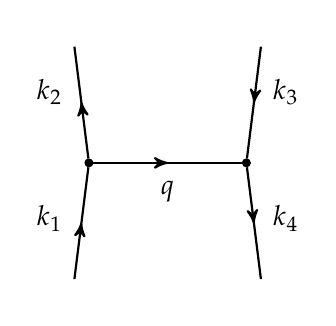
\begin{tikzpicture}[anchor=base,baseline]
		\node (vertL) at (-1,0) [twopt] {};
		\node (vertR) at ( 1,0) [twopt] {};
		\node (opO1) at (-1.2,-1.6) [] {};
		\node (opO2) at (-1.2, 1.6) [] {};
		\node (opO3) at ( 1.2, 1.6) [] {};
		\node (opO4) at ( 1.2,-1.6) [] {};
		\node at (-1.5,-0.8) {$k_1$};
		\node at (-1.5,0.8) {$k_2$};
		\node at (1.5,0.8) {$k_3$};
		\node at (1.5,-0.8) {$k_4$};
		\node at (0,-0.4) {$q$};
		\draw [spinning] (opO1) -- (vertL);
		\draw [spinning] (vertL)-- (opO2);
		\draw [spinning] (vertL)-- (vertR);
		\draw [spinning] (opO3) -- (vertR);
		\draw [spinning] (vertR)-- (opO4);
	\end{tikzpicture}}
	\eeq
and the amplitude can be expressed in terms of the Mandelstam variables
	\beq
		s=-(k_1+k_3)^2\,, \qquad t= -(k_1-k_2)^2\,.
	\eeq
The amplitude now depends only on $s$ and the momentum exchange $q$ in the transverse directions, because we are considering the following configuration of null momenta, written in light-cone coordinates $p=(p^u,p^v,p_\perp)$
	\bea
		k_1^\mu &= \left( k^u, \frac{q^2}{4 k^u},\frac{q}{2} \right)\,, \qquad
		&& k_3^\mu = \left( \frac{q^2}{4k^v},k^v,-\frac{q}{2} \right)\,, \\
		k_2^\mu &= \left( k^u, \frac{q^2}{4 k^u},-\frac{q}{2} \right)\,, \qquad
		&& k_4^\mu = \left( \frac{q^2}{4 k^v},k^v,\frac{q}{2} \right)\,.
	\eea{eq:external_momenta} 
Notice that we reserve the letter $q$ for $(D-2)$-dimensional vectors in the transverse momentum space.
In the Regge limit $k^u \sim k^v \to \infty$ the  Mandelstams are given by 
	\beq
		s\approx k^u k^v \,, \qquad t=-q^2\,.
		\label{eq:impact_mandelstams}
	\eeq
The tensor structures in such amplitudes are fixed in terms of the on-shell three-point amplitudes.
For the case with two external scalars
and an intermediate particle (labeled $I$) with spin $J$
there is only one possible tensor structure for the three-point amplitudes given by
	\beq
		  \tilde{A}^{12I} = a_J (\e_I \cdot k_1)^{J}\,, \qquad \qquad
		  \tilde{A}^{34I} = a_J (\e_I \cdot k_3)^{J}
		\,,
	\eeq
where we encode traceless and transverse polarization tensors in terms of
vectors satisfying $\e_i^2 =  \e_i \cdot k_i = 0$.
We can then   write the four-point amplitude as
	\beq
		 A_{(m,J)} (s,t)=  
		\frac{\sum_{\e_I} \tilde{A}^{12I} \tilde{A}^{34I}}{t-m^2}\approx
		  \frac{a_J^2\, s^J}{t-m^2} \,,
		\label{eq:A_spinning_flat}
	\eeq
where  we used that for large $s$ the sum over polarizations is dominated by $\e_{Iu} k_1^u \sim k^u$ and $\e_{Iv} k_3^v \sim k^v$.
The $s^J$ behavior is naively problematic at high energies, especially if the spectrum contains particles of large spin, as is the case in string theory. However, boundedness of the amplitude in the Regge limit means there is a delicate balance between the infinitely many contributions in the sum over spin.\footnote{The couplings $a_J$  are dimensionful,  $[a_J]= 3- D/2 -J$, and accommodate for higher derivatives in the couplings to higher spin fields. In string theory the dimensionful scale is $\alpha'$ and the dimensionless couplings are all proportional to the string coupling $g_s$.} The precise framework to describe this phenomenon is Regge theory \cite{Regge:1959mz}, which was reviewed for flat space in \cite{Costa:2012cb,Caron-Huot:2020nem}.

In the Regge limit one has to consider the particle with the maximum spin $j(m^2)$ for each mass. The function $j(m^2)$ is called the leading Regge trajectory and the contributions from these particles get resummed into an effective particle with continuous spin $j(t)$.
In this work we will focus on the leading trajectory with   vacuum  quantum numbers known as the Pomeron.
At tree-level the amplitude for Pomeron exchange factorizes into three-point amplitudes involving a Pomeron and the universal Pomeron propagator $\b(t)$. For example,  in the case of 4-dilaton scattering in type IIB strings we have
\beq
 A_\text{tree} (s,t)  =   \frac{8 }{\alpha'} A^{12P} \beta(t) A^{34P} \left(\frac{\alpha's}{4}\right)^{j(t)}\,,
\label{eq:A_tree_regge}
\eeq
with
	\beq
		\beta(t) =   2 \pi^2 \frac{\Gamma(- \frac{\a'}{4} t)}{\Gamma(1+\frac{\a'}{4} t)}\,
		e^{- \frac{i \pi \a'}{4} t} \,.
		\label{eq:pomeron_propagator}
	\eeq
$A^{ijP}$ are the three-point amplitudes between the external scalars and the Pomeron with the 
 $s$-dependence factored out and normalized such that in the case of 4-dilaton scattering   $A^{ijP}=1$. 
 This is convenient since later on, when we consider more general string states with spin, 
the string three-point amplitudes defined this way will contain just tensor structures.
Diagrammatically we can write (\ref{eq:A_tree_regge}) as
\beq
	\diagramEnvelope{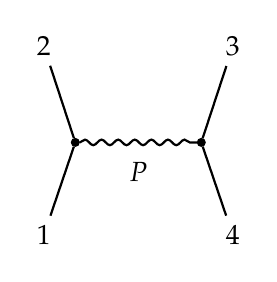
\begin{tikzpicture}[anchor=base,baseline]
		\node (vertL) at (-0.8,0.1) [twopt] {};
		\node (vertR) at ( 0.8,0.1) [twopt] {};
		\node (opO1) at (-1.2,-1.2) [] {$1$};
		\node (opO2) at (-1.2, 1.2) [] {$2$};
		\node (opO3) at ( 1.2, 1.2) [] {$3$};
		\node (opO4) at ( 1.2,-1.2) [] {$4$};
		\node at (0,-0.4) {$P$};
		\draw [spinning no arrow] (opO1) -- (vertL);
		\draw [spinning no arrow] (vertL)-- (opO2);
		\draw [finite] (vertL)-- (vertR);
		\draw [spinning no arrow] (opO3) -- (vertR);
		\draw [spinning no arrow] (vertR)-- (opO4);
	\end{tikzpicture}}
=
	\diagramEnvelope{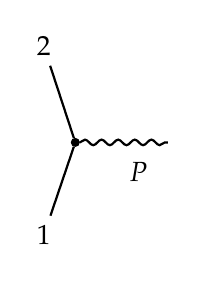
\begin{tikzpicture}[anchor=base,baseline]
		\node (vertL) at (-0.8,0.1) [twopt] {};
		\node (vertR) at ( 0.5,0.1) [] {};
		\node (opO1) at (-1.2,-1.2) [] {$1$};
		\node (opO2) at (-1.2, 1.2) [] {$2$};
		\node at (0,-0.4) {$P$};
		\draw [spinning no arrow] (opO1) -- (vertL);
		\draw [spinning no arrow] (vertL)-- (opO2);
		\draw [finite] (vertL)-- (vertR);
	\end{tikzpicture}}
\times
	\diagramEnvelope{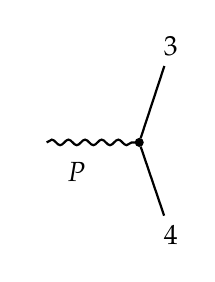
\begin{tikzpicture}[anchor=base,baseline]
		\node (vertL) at (-0.5,0.1) [] {};
		\node (vertR) at ( 0.8,0.1) [twopt] {};
		\node (opO3) at ( 1.2, 1.2) [] {$3$};
		\node (opO4) at ( 1.2,-1.2) [] {$4$};
		\node at (0,-0.4) {$P$};
		\draw [finite] (vertL)-- (vertR);
		\draw [spinning no arrow] (opO3) -- (vertR);
		\draw [spinning no arrow] (vertR)-- (opO4);
	\end{tikzpicture}}
\times \frac{2 G_N}{\pi}  \frac{8 }{\alpha'}
\,\b(t) \left(\frac{\alpha's}{4}\right)^{j(t)}
\,.
\label{eq:Pomeron_factorization}
\eeq
Amplitudes involving a Pomeron can be computed in string theory using the Pomeron vertex operator \cite{Ademollo:1989ag,Ademollo:1990sd,Brower:2006ea}. The factorization into three-point functions and a Pomeron propagator holds for general external string states \cite{Brower:2006ea,DAppollonio:2013mgj}.

%%%%%%%%%%%%%%%%%%%%%%%%%%%%%%%%%%%%%%%%%%%%%%%%%%%%%%%%%%%%%%%%%%%%%%%%%%%%%%%%%
\subsection{Optical theorem and impact parameter space}
\label{sec:impact_optical_theorem_flat}
%%%%%%%%%%%%%%%%%%%%%%%%%%%%%%%%%%%%%%%%%%%%%%%%%%%%%%%%%%%%%%%%%%%%%%%%%%%%%%%%%

Next we consider the expression for the two-line cut of the one-loop amplitude in the impact parameter representation, which will be given in terms of the tree-level pieces we have discussed so far.
The two-line cut receives a contribution from two-Pomeron exchange, which is the leading term in the Regge limit of the one-loop amplitude.
Consider the following configuration of momenta
	\beq
	\diagramEnvelope{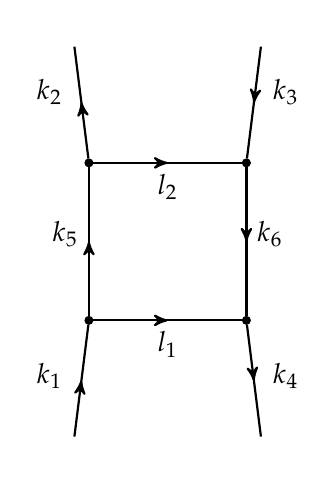
\begin{tikzpicture}[anchor=base,baseline]
		\node (vert1) at (-1,-1) [twopt] {};
		\node (vert2) at (-1, 1) [twopt] {};
		\node (vert3) at ( 1, 1) [twopt] {};
		\node (vert4) at ( 1,-1) [twopt] {};
		\node (opO1) at (-1.2,-2.6) [] {};
		\node (opO2) at (-1.2, 2.6) [] {};
		\node (opO3) at ( 1.2, 2.6) [] {};
		\node (opO4) at ( 1.2,-2.6) [] {};
		\node at (-1.5,-1.8) {$k_1$};
		\node at (-1.5,1.8) {$k_2$};
		\node at (1.5,1.8) {$k_3$};
		\node at (1.5,-1.8) {$k_4$};
		\node at (0,-1.4) {$l_1$};
		\node at (0,0.6) {$l_2$};
		\node at (-1.3,0) {$k_5$};
		\node at (1.3,0) {$k_6$};
		\draw [spinning] (opO1) -- (vert1);
		\draw [spinning] (vert2) -- (opO2);
		\draw [spinning] (opO3) -- (vert3);
		\draw [spinning] (vert4) -- (opO4);
		\draw [spinning] (vert1) -- (vert2);
		\draw [spinning] (vert1) -- (vert4);
		\draw [spinning] (vert2) -- (vert3);
		\draw [spinning] (vert3) -- (vert4);
	\end{tikzpicture}}\,.
\label{fig:momenta_1loop}
	\eeq
The external momenta are again in the configuration \eqref{eq:external_momenta} with Mandelstams \eqref{eq:impact_mandelstams}.
The optical theorem tells us to cut the internal lines of the diagram, putting the corresponding legs on-shell. This implies the following equation for the discontinuity of the amplitude
	\beq
	2 \Im A_{\text{1-loop}}(s,q) = \! \sum\limits_{\substack{m_5,\rho_5,\e_5\\m_6,\rho_6,\e_6}}
	\int \! \frac{d l_1}{(2 \pi)^{D}} \, 2\pi i \de(k_5^2 + m_5^2) \, 2\pi i \de(k_6^2 + m_6^2) 
	A_\text{tree}^{3652} (s,l_2)^*
	A_\text{tree}^{1564} (s,l_1)\,,
	\label{eq:optical_theorem_start}
	\eeq
where one sums over all possible particles 5 and 6 with masses $m$, in Little group representations $\rho$ and with 
polarization tensors $\e$. The sums over polarizations can be evaluated using completeness relations.
In order to remove the delta functions we express $k_5$ and $k_6$ in terms of $l_1$ and the external momenta \eqref{eq:external_momenta}.
Then we write the loop momentum as $l_1^\mu = (l^u,l^v,q_1)$
and use the delta-functions to fix the forward components of the loop momentum $l_u$ and $l_v$ to
\bea
l^u = \frac{m_6^2 +q_1^2 +q \cdot q_1}{ k^v}\,,
		    \qquad\qquad
l^v = -\frac{m_5^2 +q_1^2 -q \cdot q_1}{ k^u}\,,
\eea{eq:onshell_solutions_flat}
leaving only the transverse integration over $q_1$.
We arrive at the equation
	\beq
		\Im A_{\text{1-loop}}(s,q) = \sum\limits_{\substack{m_5,\rho_5,\e_5\\m_6,\rho_6,\e_6}}
		\int \frac{dq_1 dq_2}{(2 \pi)^{D-2}}  \, \frac{\de(q-q_1-q_2)}{4 s}
		A_\text{tree}^{3652} (s,q_2)^*
		A_\text{tree}^{1564} (s,q_1)\,,
		\label{eq:optical_theorem_flat}
	\eeq
where we introduced the transverse momentum $q_2=q-q_1$  to write the expression 
in a more symmetrical way. 	
Using that the tree-level amplitudes are given 
in the Regge limit by Pomeron exchange, we can write (\ref{eq:optical_theorem_flat}) diagrammatically as in figure \ref{fig:optical_theorem_flat}.
\begin{figure}
\begin{equation*}
	\diagramEnvelope{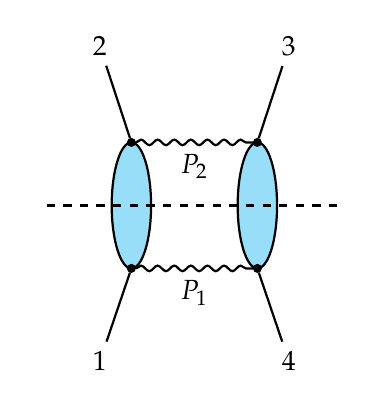
\begin{tikzpicture}[anchor=base,baseline]
        \draw [thick,fill=cyan,fill opacity=0.4] (-0.8,0.1) ellipse (0.25 and 0.8);
        \draw [thick,fill=cyan,fill opacity=0.4] (0.8,0.1) ellipse (0.25 and 0.8);
		\node (vert1) at (-.8,-.7) [twopt] {};
		\node (vert2) at (-.8, .9) [twopt] {};
		\node (vert3) at ( .8, .9) [twopt] {};
		\node (vert4) at ( .8,-.7) [twopt] {};
        \node (cut1) at (-2,.1) [] {};
        \node (cut2) at (2,.1) [] {};
		\node (opO1) at (-1.2,-2) [] {$1$};
		\node (opO2) at (-1.2, 2) [] {$2$};
		\node (opO3) at ( 1.2, 2) [] {$3$};
		\node (opO4) at ( 1.2,-2) [] {$4$};
		\node at (0,-1.1) {$P_1$};
		\node at (0,0.5) {$P_2$};
		\draw [spinning no arrow] (opO1) -- (vert1);
		\draw [spinning no arrow] (vert2) -- (opO2);
		\draw [spinning no arrow] (opO3) -- (vert3);
		\draw [spinning no arrow] (vert4) -- (opO4);
		\draw [finite] (vert1) -- (vert4);
		\draw [finite] (vert2) -- (vert3);
		\draw [scalar no arrow] (cut1) -- (cut2);
	\end{tikzpicture}}
\sim
\sum\limits_{\substack{m_5,\rho_5,\e_5\\m_6,\rho_6,\e_6}} \int
	\diagramEnvelope{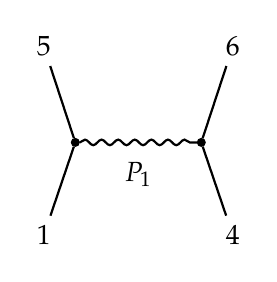
\begin{tikzpicture}[anchor=base,baseline]
		\node (vertL) at (-0.8,0.1) [twopt] {};
		\node (vertR) at ( 0.8,0.1) [twopt] {};
		\node (opO1) at (-1.2,-1.2) [] {$1$};
		\node (opO2) at (-1.2, 1.2) [] {$5$};
		\node (opO3) at ( 1.2, 1.2) [] {$6$};
		\node (opO4) at ( 1.2,-1.2) [] {$4$};
		\node at (0,-0.4) {$P_1$};
		\draw [spinning no arrow] (opO1) -- (vertL);
		\draw [spinning no arrow] (vertL)-- (opO2);
		\draw [finite] (vertL)-- (vertR);
		\draw [spinning no arrow] (opO3) -- (vertR);
		\draw [spinning no arrow] (vertR)-- (opO4);
	\end{tikzpicture}}
\times
	\diagramEnvelope{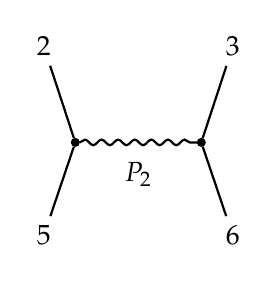
\begin{tikzpicture}[anchor=base,baseline]
		\node (vertL) at (-0.8,0.1) [twopt] {};
		\node (vertR) at ( 0.8,0.1) [twopt] {};
		\node (opO1) at (-1.2,-1.2) [] {$5$};
		\node (opO2) at (-1.2, 1.2) [] {$2$};
		\node (opO3) at ( 1.2, 1.2) [] {$3$};
		\node (opO4) at ( 1.2,-1.2) [] {$6$};
		\node at (0,-0.4) {$P_2$};
		\draw [spinning no arrow] (opO1) -- (vertL);
		\draw [spinning no arrow] (vertL)-- (opO2);
		\draw [finite] (vertL)-- (vertR);
		\draw [spinning no arrow] (opO3) -- (vertR);
		\draw [spinning no arrow] (vertR)-- (opO4);
	\end{tikzpicture}}
\end{equation*}
\caption{Optical theorem in the Regge limit in terms of Feynman diagrams. The tree-level correlators are dominated by $s$-channel Pomeron exchange. The ellipses on the l.h.s.\ indicate that all string excitations are taken into account.}
\label{fig:optical_theorem_flat}	
\end{figure}
The optical theorem can be simplified even further by transforming it to impact parameter space. To this end the amplitude is expressed in terms of the impact parameter $b$, which is a vector in the transverse impact  parameter space $\mathbb{R}^{D-2}$, using the following transformation
	\beq
		\de (s,b) = \frac{1}{2s} \int \frac{d q}{(2\pi)^{D-2}} \,e^{i  q\cdot b}  A(s,t)\,.
		\label{eq:impact_flat}
	\eeq
We can use this definition together with \eqref{eq:optical_theorem_flat} to compute
	\bea
		\Im  \de_{\text{1-loop}}(s,b)  %={}&
		={}& \frac{1}{2} \sum\limits_{\substack{m_5,\rho_5,\e_5\\m_6,\rho_6,\e_6}}
		\de_\text{tree}^{3652}(s,-b)^* \,\de_\text{tree}^{1564}(s,b)\,.
	\eea{eq:impact_optical_theorem}
We conclude that the impact parameter representation absorbs the remaining phase space integrals in the optical theorem, resulting in a purely multiplicative formula. In fact, in the case where the particles on the left and right of the diagram do not change (i.e.\ 1,5,2 and 3,6,4 are identical particles), such a statement holds to all-loops, leading to exponentiation of the tree-level phase shift, which is the basis for the famous eikonal approximation.

%%%%%%%%%%%%%%%%%%%%%%%%%%%%%%%%%%%%%%%%%%%%%%%%%%%%%%%%%%%%%%%%%%%%%%%%%%%%%%%%%
\subsection{Vertex function}
\label{sec:vertex_function_flat}
%%%%%%%%%%%%%%%%%%%%%%%%%%%%%%%%%%%%%%%%%%%%%%%%%%%%%%%%%%%%%%%%%%%%%%%%%%%%%%%%%

Another notion we will use is that of the vertex function, which arises when combining
the optical theorem \eqref{eq:optical_theorem_flat} with the factorization of the tree-level amplitudes \eqref{eq:A_tree_regge} into three-point amplitudes. By combining the two results one sees that the sums over particles and their polarizations factorize into separate sums for particles 5 and 6, which we call the vertex function $V$
\beq
V(q_1,q_2) \equiv \sum\limits_{m_5,\rho_5,\e_5} A^{15P_1}(q_1) A^{25P_2}(q_2)\,.
\label{eq:V_flat_def}
\eeq
Moreover, such a sum over representations and polarizations for each mass is given by tree-level unitarity as the residue of the four-point amplitudes with two external Pomerons
\beq
\underset{k_5^2=-m_5^2}\Res A^{12 P_1 P_2}(k_5,q_1,q_2) = \sum\limits_{\rho_5,\e_5} A^{15P_1}(q_1) A^{25P_2}(q_2)\,.
\label{eq:residue_generic}
\eeq
In terms of diagrams this reads
\beq
V(q_1,q_2) \equiv \sum\limits_{m_5,\rho_5,\e_5}
	\diagramEnvelope{\begin{tikzpicture}[anchor=base,baseline]
		\node (vertU) at (0,0.9) [] {$5$};
		\node (vertD) at (0,-0.3) [twopt] {};
		\node (opO1) at (-1.2,-0.8) [] {$1$};
		\node (opOP1) at ( 1.2,-0.8) [] {$P_1$};
		\draw [spinning no arrow] (opO1) -- (vertD);
		\draw [spinning no arrow] (vertU)-- (vertD);
		\draw [finite] (vertD)-- (opOP1);
	\end{tikzpicture}}
\times
	\diagramEnvelope{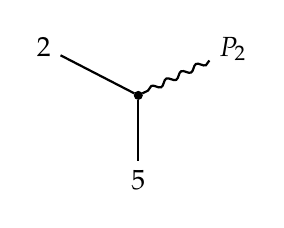
\begin{tikzpicture}[anchor=base,baseline]
		\node (vertU) at (0,0.4) [twopt] {};
		\node (vertD) at (0,-0.8) [] {$5$};
		\node (opO2) at (-1.2, 0.9) [] {$2$};
		\node (opOP2) at ( 1.2, 0.9) [] {$P_2$};
		\draw [spinning no arrow] (vertU)-- (opO2);
		\draw [spinning no arrow] (vertU)-- (vertD);
		\draw [finite] (opOP2) -- (vertU);
	\end{tikzpicture}}
=\sum\limits_{m_5} \underset{k_5^2=-m_5^2}\Res
	\diagramEnvelope{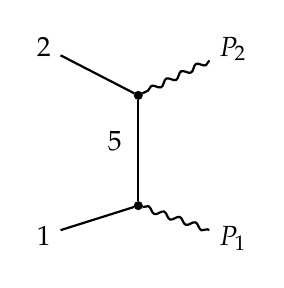
\begin{tikzpicture}[anchor=base,baseline]
		\node (vertU) at (0,0.7) [twopt] {};
		\node (vertD) at (0,-0.7) [twopt] {};
		\node (opO1) at (-1.2,-1.2) [] {$1$};
		\node (opO2) at (-1.2, 1.2) [] {$2$};
		\node (opOP2) at ( 1.2, 1.2) [] {$P_2$};
		\node (opOP1) at ( 1.2,-1.2) [] {$P_1$};
		\node at (-.3,0) {$5$};
		\draw [spinning no arrow] (opO1) -- (vertD);
		\draw [spinning no arrow] (vertU)-- (opO2);
		\draw [spinning no arrow] (vertU)-- (vertD);
		\draw [finite] (opOP2) -- (vertU);
		\draw [finite] (vertD)-- (opOP1);
	\end{tikzpicture}}\,.
\label{eq:V_diagrams}
\eeq
The vertex function combines all information about the exchanges of possibly spinning particles 5 and 6 into a single scalar function. In terms of the vertex function the optical theorem \eqref{eq:optical_theorem_flat} in the Regge limit becomes
\begin{align}
\Im A_{\text{1-loop}}(s,q) =  -\frac{1}{4s} 
&\int  \frac{dq_1  dq_2}{(2\pi)^{D-2}} \, \de(q-q_1-q_2)
\label{eq:optical_theorem_V_flat}
\\
&\left( \frac{8}{\alpha'}\right)^2 \b(t_1)^* \b(t_2) V(q_1,q_2)^2 \left(\frac{\alpha's}{4}\right)^{j(t_1) + j(t_2)}\,,
\nonumber
\end{align}
where $t_i = -q_i^2$.

%%%%%%%%%%%%%%%%%%%%%%%%%%%%%%%%%%%%%%%%%%%%%%%%%%%%%%%%%%%%%%%%%%%%%%%%%%%%%%%%%
\subsection{Spinning three-point amplitudes}
\label{sec:3pt_amplitudes}
%%%%%%%%%%%%%%%%%%%%%%%%%%%%%%%%%%%%%%%%%%%%%%%%%%%%%%%%%%%%%%%%%%%%%%%%%%%%%%%%%









Since it will be important later to compare tensor structures in AdS and flat space, we will provide here some more details on the tensor structures of the three-point amplitudes that appear in the unitarity cut of the four-point amplitude $A^{12 P_1 P_2}$ discussed above.
The external momentum $k_1$ and the exchanged momentum $l_1$, with light-cone components given in the Regge limit by
(\ref{eq:onshell_solutions_flat}), fix the momentum $k_5=k_1-l_1$ as shown in the figure below. We may, however, change frame such that 
$k_5$ has no transverse momentum \cite{DAppollonio:2013mgj}. Such change of frame does not alter the fact that the light-cone components of $l_1$ are 
subleading. The same applies to $l_2$. Thus in the Regge limit we can safely write
\beq
	\diagramEnvelope{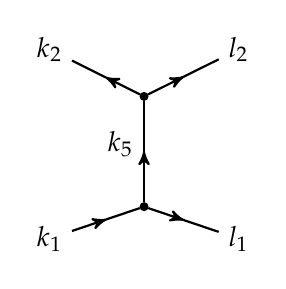
\begin{tikzpicture}[anchor=base,baseline]
		\node (vertU) at (0,0.7) [twopt] {};
		\node (vertD) at (0,-0.7) [twopt] {};
		\node (opO1) at (-1.2,-1.2) [] {$k_1$};
		\node (opO2) at (-1.2, 1.2) [] {$k_2$};
		\node (opOP2) at ( 1.2, 1.2) [] {$l_2$};
		\node (opOP1) at ( 1.2,-1.2) [] {$l_1$};
		\node at (-.3,0) {$k_5$};
		\draw [spinning] (opO1) -- (vertD);
		\draw [spinning] (vertU)-- (opO2);
		\draw [spinning] (vertD)-- (vertU);
		\draw [spinning] (vertU) -- (opOP2);
		\draw [spinning] (vertD)-- (opOP1);
	\end{tikzpicture}}
\qquad \quad
\begin{aligned}
k_5 &\approx  \left( k_5^u ,\frac{m_5^2}{k_5^u},0 \right)\,, &\\
l_2 &\approx  (0,0, q_2)\,, \qquad& k_2 = k_5 - l_2\,, \\
l_1 &\approx  (0,0, q_1)\,, \qquad& k_1 = k_5 + l_1 \,.
\end{aligned}
\eeq
We focus on the three-point amplitude $A^{15P_1}(q_1)$, which is related to the four-point amplitude via the tree-level unitarity \eqref{eq:residue_generic}.
In this relation we have a sum over a basis of possible polarizations $\e_5$,
which can be evaluated using completeness relations, e.g.\ for massive bosons \cite{Boels:2014dka}
	\beq
		\sum\limits_{\e_5} \e_{5}^{\mu_1 \ldots \mu_{|\rho|}}
		\e_{5}^{\nu_1 \ldots \nu_{|\rho|}} 
		= P^{\mu_1}_{5 \g_1} \ldots P^{\mu_{\rho}}_{5 \g_{\rho}}
		%
		\pi_\rho^{\g_1 \ldots \g_{|\rho|}; \,\s_1 \ldots \s_{|\rho|}}
		P^{\nu_1}_{5 \s_1} \ldots P^{\nu_{\rho}}_{5 \s_{\rho}} \,,
		\label{eq:completeness_relation}
	\eeq
where $\pi_\rho$ is the projector to the irreducible $SO(D-1)$ representation $\rho$ and
	\beq
		P_{5 \nu}^{\mu} = \de^{\mu}_{\nu} - \frac{k_{5}^{\mu} k_{5 \nu}}{k_5^2}\,,
	\eeq
is a projector to the space transverse to $k_5$.
We will always absorb the projectors $P_{5 \nu}^{\mu}$ into the three-point amplitudes, i.e.\ consider amplitudes in a transverse configuration. That means that the indices corresponding to particle 5 have to be constructed from the projected momenta of the other particles, which are identical
\beq
P_{5 \nu}^{\mu} l_{1\mu} = P_{5 \nu}^{\mu} k_{1\mu}\,.
\label{eq:P5l}
\eeq
Apart from that, massive particles can also have a longitudinal polarization $v$ which satisfies
\beq
v \cdot k_5 = 0 \,, \qquad v^2 = 1\,,
\eeq
and is given in this frame explicitly by
\beq
v_\mu =\frac{1}{m_5} \left(  k_5^u, - \frac{m_5^2}{k_5^u},  0 \right)\,.
\eeq
For the case that particle 1 is a scalar, we can then construct $A^{15P}$ in terms of the following manifestly transverse tensor structures
	\beq
		A^{15P}_{m_5,\rho_5,\bmu} = \sum\limits_{k=0}^{|\rho_5|} 
		a_{m_5,\rho_5}^{k}(t_1) \,
i^{|\rho_5|} \sqrt{\a'}^{|\rho_5|-k}
v_{\mu_1} \ldots v_{\mu_k} q_{1\mu_{k+1}} \ldots q_{1\mu_{|\rho_5|}}\,,
		\label{eq:3pt_spinning}
	\eeq
where we introduced boldface indices $\bmu$ as multi-indices that stand for the $|\rho|$ indices for the irrep $\rho$.	
By abuse of language we defined the vector $q_1\equiv(0,0,q_1)$, since $q_1$ is transverse.
If particle 1 carries spin as well, as will be the case for the gravitons considered later on, we construct the polarization tensors out of the vector $\xi_1=(\xi_1^u, \xi_1^v, \e_1)$. In this case, again defining
$\epsilon_1\equiv (0,0,\epsilon_1)$, the amplitudes take the following form in the Regge limit
	\bea
		A^{15P}_{m_5,\rho_5,\bmu} =  \sum\limits_{n=0}^{\ell_1}  \sum\limits_{k=0}^{|\rho_5|-n}
		&a_{m_5,\rho_5}^{k,n}(t_1) \,
i^{|\rho_5|} 
\sqrt{\a'}^{|\rho_5|+\ell_1-2n-k}
(\e_1\cdot q_1)^{\ell_1 - n}
\\
& \e_{1\mu_1} \ldots \e_{1\mu_n}  v_{\mu_{n+1}} \ldots v_{\mu_{n+k}} q_{1\mu_{n+k+1}} \ldots q_{1\mu_{|\rho_5|}}\,,
	\eea{eq:3pt_spinning_more}
as can be checked by comparing with the explicit amplitudes computed in \cite{DAppollonio:2013mgj}. These choices for the tensor structures are particularly convenient since $q_1 \cdot v = \e_1 \cdot v = 0$. Contact with the momentum frame used in the previous subsections is made by identifying the Lorentz invariant $A^{12 P_1 P_2}$.


\section{AdS impact parameter space}
\label{sec:ads}


Our goal in this section is to compute the Regge limit of a scalar four-point function in a perturbative large $N$ CFT at one-loop and finite
$\Delta_{\text{gap}}$. At finite $\Delta_{\text{gap}}$ we have to consider the $t$-channel exchange of all possible double-trace operators and also single-trace operators, which are respectively dual to tidal excitations of the external scattering states and  to long-string creation in the string theory context. It was shown in \cite{Meltzer:2019pyl} that the exchange of single-trace operators dual to the long-string creation effects is subleading in the Regge limit. Therefore we only need to consider the exchange of double-trace operators.
This is where the new perturbative CFT optical theorem \eqref{eq:cft_optical_theorem_intro} takes a central role, as it allows us to compute the contributions of double-trace operators to the correlator starting from the corresponding tree-level correlators. The contribution of the leading Regge trajectory to the scalar tree-level correlators is known to leading order in the Regge limit \cite{Cornalba:2007fs,Costa:2012cb}.

In this section we will therefore study \eqref{eq:cft_optical_theorem_intro} in the Regge limit, and this time we expand the tree-level correlators in the $s$-channel. In the Regge limit the four external points are
in Lorentzian kinematics as depicted in figure \ref{fig:regge_figure}.
\begin{figure}
    \begin{center}
        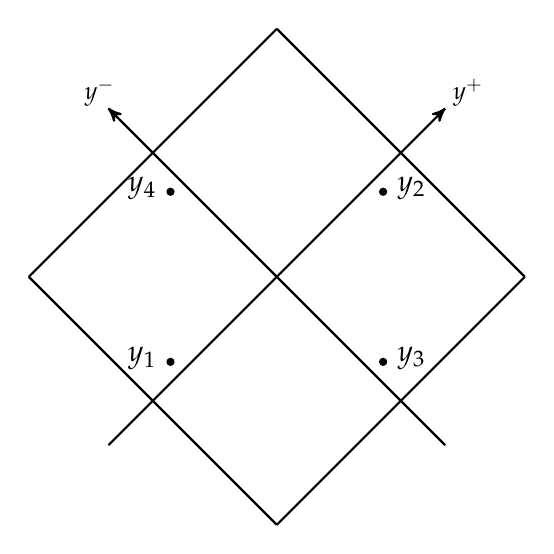
\begin{tikzpicture}[anchor=base,baseline,scale=0.9, transform shape]
            \node (vertLT) at (-2.5, 2.5) [] {};
            \node (vertRT) at ( 2.5, 2.5) [] {};
            \node (vertLB) at (-2.5,-2.5) [] {};
            \node (vertRB) at ( 2.5,-2.5) [] {};
            \node (opO1) at (-1.2,-1.6) [] {};
            \node (opO2) at (-1.2, 1.6) [] {};
            \node (opO3) at ( 1.2,-1.6) [] {};
            \node (opO4) at ( 1.2, 1.6) [] {};
            \node at (-1.9,-1.2) {\large $y_1$};
            \node at (-1.9,1.2) {\large $y_4$};
            \node at (1.9,-1.2) {\large $y_3$};
            \node at (1.9,1.2) {\large $y_2$};
            \node at (-1.5,-1.2) [twopt] {};
            \node at (-1.5,1.2) [twopt] {};
            \node at (1.5,-1.2) [twopt] {};
            \node at (1.5,1.2) [twopt] {};
            \node at (2.7,2.5) {$y^+$};
            \node at (-2.5,2.5) {$y^-$};
            \draw [axis] (vertLB)-- (vertRT);
            \draw [axis] (vertRB)-- (vertLT);
            \draw [thick, black] (0,3.5) -- (-3.5,0);
            \draw [thick, black] (0,-3.5) -- (-3.5,0);
            \draw [thick, black] (3.5,0) -- (0,3.5);
            \draw [thick, black] (3.5,0) -- (0,-3.5);
        \end{tikzpicture}
    \end{center}
    \caption{Kinematics in the central Poincar\'{e} patch with coordinates $y_i$. Time is on the vertical axis, transverse directions are suppressed.}
    \label{fig:regge_figure}
\end{figure}
In this configuration all distances between points are spacelike except for $y_{14}^2, y_{23}^2 < 0$.
The Regge limit is reached by sending the four-points to infinity along the light cones
\beq
y_{1}^{+} \rightarrow-\infty, \quad y_{2}^{+} \rightarrow+\infty, \quad y_{3}^{-} \rightarrow-\infty, \quad y_{4}^{-} \rightarrow+\infty\,.
\eeq
The Regge limit can be directly applied to the left hand side of \eqref{eq:cft_optical_theorem_intro}. The terms on the Regge sheets $A^{\circlearrowleft}(y_i)$ and $A^{\circlearrowright}(y_i)$ are dominant over the Euclidean terms in this limit. However, we cannot apply the Regge limit directly to the right hand side of \eqref{eq:cft_optical_theorem_intro} as the shadow integrals range over Euclidean configurations. Hence we will apply Wick rotations on the points $y_{5},\,y_{6},\,y_{7},\,y_{8}$ to obtain a gluing of the discontinuities of Lorentzian correlators. We will assume that in the Regge limit the dominant contribution to the gluing formula comes from the domain where the individual tree-level correlators are in the Regge limit themselves. We do not provide a proof of this assumption but we justify it in section \ref{sec:reggeandimpact}.

When each four-point function in \eqref{eq:gluing_expan} is in the Regge limit, the points $y_{5},\,y_{6},\,y_{7},\,y_{8}$ are placed in the same positions as $y_{1},\,y_{4},\,y_{2},\,y_{3}$ in fig.\ \ref{fig:regge_figure}, respectively. Thus $y_7$ is in the future of $y_8$ and this pair is spacelike from $y_1 ,\, y_4 ,\, y_5 ,\, y_6$. Similarly, $y_6$ is in the future of $y_5$ and is spacelike from $y_2 ,\, y_3 ,\, y_7 ,\, y_8$.
For the chosen kinematics
we put the pair $y_5 ,\, y_6$ in anti-time order  using the epsilon prescription of \eqref{eq:wightman} with $\epsilon_5 > \epsilon_6$, and the pair $y_7 ,\, y_8$ in time order using $\epsilon_7 > \epsilon_8$. Applying this on \eqref{eq:cft_optical_theorem} gives the following formula for the Regge limit of the double discontinuity
\begin{align}
    \dDisc_t A_{\text{1-loop}}(y_k) \Big|_{\text{d.t.}} = -\frac{1}{2}
    \sum\limits_{\cO_5, \cO_6}  \frac{1}{N_{\cO_5}N_{\cO_6}}\int & dy_5 dy_6 dy_7 dy_8\, \< [\cO_2 ,\cO_3 ] \cO_5 \cO_6 \>_{\text{tree}} \< \tl \cO_5 \tl{\cO}_{7}^{\dag}\>  \nonumber \\
                                                                 & \<\tl \cO_6 \tl{\cO}_{8}^{\dag}\>
    \< \cO_7 \cO_8 [\cO_4 , \cO_1]\>_{\text{tree}} \Big|_{\left[\cO_5\cO_6\right]} \,.
    \label{eq:regge_gluing_form}
\end{align}
The relative ordering between $\epsilon_5 ,\epsilon_7$ and $\epsilon_6 ,\epsilon_8$ is irrelevant as the pairs, appearing in the two-point functions on the right hand side of \eqref{eq:regge_gluing_form}, are spacelike separated in the Regge configuration.

In this section we define the discontinuities as the commutators inserted into the fully Lorentzian correlators
\bea
\Disc_{14} A^{1874}(y_i) &\coloneqq \< \cO_7 \cO_8 [\cO_4 , \cO_1]\> =
A^{1874}{}^\circlearrowleft(y_i) - A^{1874}_{\text{Euc}}(y_i)\,, \\
\Disc_{23}  A^{3652}(y_i) &\coloneqq \< [\cO_2 ,\cO_3 ] \cO_5 \cO_6 \> =
A^{3652}_{\text{Euc}}(y_i) - A^{3652}{}^\circlearrowright(y_i)  \,.
\label{eq:new_singledisc}\end{aligned}\end{equation}
This definition differs slightly from the one in \eqref{eq:discdefnorg}. Stripping out the appropriate pre-factors from \eqref{eq:new_singledisc}, one can check that these single discontinuities can be equivalently defined as
\bea
\Disc_{14}  \mathcal{A}^{1234}(z,\bar{z}) &\coloneqq
e^{i \pi(a+b)} \mathcal{A}^{1234}(z,\bar{z}^\circlearrowleft) - e^{-i \pi(a+b)} \mathcal{A}^{1234}(z,\bar{z})\,, \\
\Disc_{23}  \mathcal{A}^{1234}(z,\bar{z}) &\coloneqq
\mathcal{A}^{1234}(z,\bar{z}) -  \mathcal{A}^{1234}(z,\bar{z}^\circlearrowright)\,, \\
\Disc_{23}  \mathcal{A}^{3412}(z,\bar{z}) & =
e^{-i \pi(a+b)} \mathcal{A}^{3412}(z,\bar{z}) - e^{i \pi(a+b)} \mathcal{A}^{3412}(z,\bar{z}^\circlearrowright)\,.
\label{eq:Disc_conventional}\end{aligned}\end{equation}
Starting from the discontinuity defined in \eqref{eq:discdefnorg}, these expressions result from continuing another half circle in $\zb$, so that the different terms are either evaluated at the original position or continued a full circle around 1. The extra phase comes from the additional Wick rotations.
The final  result matches the definition of the discontinuity in \cite{Caron-Huot:2020nem}.
Note that $\zb$ is continued an extra half circle in opposite directions for the first two lines in \eqref{eq:Disc_conventional}, so that with these definitions the relation to the $\dDisc$ in \eqref{eq:dDisc_y} remains valid.\footnote{For $t$-channel blocks, the new definitions for the discontinuities in \eqref{eq:Disc_conventional} are related to the old definition in \eqref{eq:discdefnorg} by a phase, for example, for $\Disc_{14}$ the relative phase is $e^{i\pi\tau_{\cO}/2}$.}
Therefore the optical theorem in the Regge limit can still be expressed as
\bea
\dDisc_t  A_{\rm 1-loop}(y_i)\Big|_\text{d.t.}  \!= -\frac{1}{2}
\sum\limits_{\substack{\mathcal{O}_5,\mathcal{O}_6\\ \in\  s.t.}}
\!
\int dy_5 dy_6 \, \Disc_{23}  A_{\rm tree}^{3652}(y_k) \, \bS_5 \bS_6 \Disc_{14} A_{\rm tree}^{1564}(y_k)  \Big|_{[\cO_5 \cO_6]}\,,
\label{eq:cft_optical_theorem_s}\end{aligned}\end{equation}
with the discontinuities as defined in the first and third lines of \eqref{eq:Disc_conventional}, and the gluing and shadow integrals now ranging over Minkowski space. This formula is also depicted in figure \ref{fig:optical_theorem_strings} in terms of Witten diagrams.
\begin{figure}
    \begin{center}
        \begin{equation*}
            \dDisc_t \,
            \diagramEnvelope{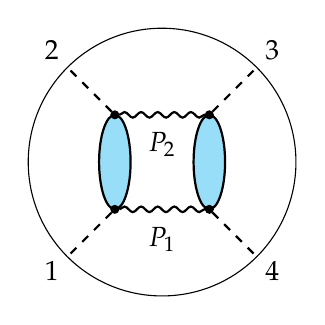
\begin{tikzpicture}[anchor=base,baseline]
                    \draw [thick,fill=cyan,fill opacity=0.4] (-0.6,0) ellipse (0.2 and 0.6);
                    \draw [thick,fill=cyan,fill opacity=0.4] (0.6,0) ellipse (0.2 and 0.6);
                    \node (vertLU) at (-0.6,0.6) [twopt] {};
                    \node (vertRU) at ( 0.6,0.6) [twopt] {};
                    \node (vertLD) at (-0.6,-0.6) [twopt] {};
                    \node (vertRD) at ( 0.6,-0.6) [twopt] {};
                    \node (opO1) at (-1.3,-1.3) [] {};
                    \node (opO2) at (-1.3, 1.3) [] {};
                    \node (opO3) at ( 1.3,-1.3) [] {};
                    \node (opO4) at ( 1.3, 1.3) [] {};
                    \node at (-1.4,-1.5) {$1$};
                    \node at (-1.4, 1.3) [] {$2$};
                    \node at ( 1.4,-1.5) [] {$4$};
                    \node at ( 1.4, 1.3) [] {$3$};
                    \node at (0,0.5) [below] {$P_2$};
                    \node at (0,-0.7) [below] {$P_1$};
                    \draw [scalar no arrow] (vertLD)-- (opO1);
                    \draw [scalar no arrow] (vertLU)-- (opO2);
                    \draw [finite] (vertLU)-- (vertRU);
                    \draw [finite] (vertLD)-- (vertRD);
                    \draw [scalar no arrow] (vertRD)-- (opO3);
                    \draw [scalar no arrow] (vertRU)-- (opO4);
                    \draw (0,0) circle (1.7);
                \end{tikzpicture}} \,
            \sim \sum\limits_{\cO_5, \cO_6} \int
            \Disc_{23}
            \diagramEnvelope{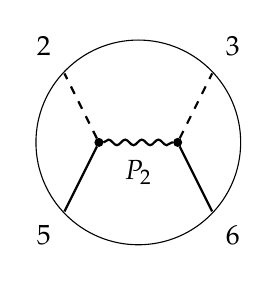
\begin{tikzpicture}[anchor=base,baseline]
                    \node (vertL) at (-0.5,0) [twopt] {};
                    \node (vertR) at ( 0.5,0) [twopt] {};
                    \node (opO1) at (-1.,-1.) [] {};
                    \node (opO2) at (-1., 1.) [] {};
                    \node (opO3) at ( 1.,-1.) [] {};
                    \node (opO4) at ( 1., 1.) [] {};
                    \node at (-1.2,-1.3) {$5$};
                    \node at (-1.2, 1.1) [] {$2$};
                    \node at ( 1.2,-1.3) [] {$6$};
                    \node at ( 1.2, 1.1) [] {$3$};
                    \node at (0,-0.1) [below] {$P_2$};
                    \draw [spinning no arrow] (vertL)-- (opO1);
                    \draw [scalar no arrow] (vertL)-- (opO2);
                    \draw [finite] (vertL)-- (vertR);
                    \draw [spinning no arrow] (vertR)-- (opO3);
                    \draw [scalar no arrow] (vertR)-- (opO4);
                    \draw (0,0) circle (1.3);
                \end{tikzpicture}}
            \Disc_{14}
            \diagramEnvelope{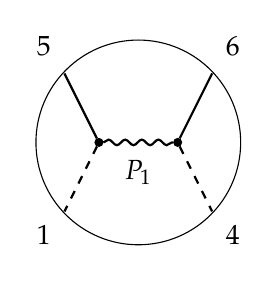
\begin{tikzpicture}[anchor=base,baseline]
                    \node (vertL) at (-0.5,0) [twopt] {};
                    \node (vertR) at ( 0.5,0) [twopt] {};
                    \node (opO1) at (-1.,-1.) [] {};
                    \node (opO2) at (-1., 1.) [] {};
                    \node (opO3) at ( 1.,-1.) [] {};
                    \node (opO4) at ( 1., 1.) [] {};
                    \node at (-1.2,-1.3) {$1$};
                    \node at (-1.2, 1.1) [] {$\tl 5$};
                    \node at ( 1.2,-1.3) [] {$4$};
                    \node at ( 1.2, 1.1) [] {$\tl 6$};
                    \node at (0,-0.1) [below] {$P_1$};
                    \draw [scalar no arrow] (vertL)-- (opO1);
                    \draw [spinning no arrow] (vertL)-- (opO2);
                    \draw [finite] (vertL)-- (vertR);
                    \draw [scalar no arrow] (vertR)-- (opO3);
                    \draw [spinning no arrow] (vertR)-- (opO4);
                    \draw (0,0) circle (1.3);
                \end{tikzpicture}}
        \end{equation*}
    \end{center}
    \caption{Optical theorem in the Regge limit in terms of Witten diagrams. The tree-level correlators are dominated by $s$-channel Pomeron exchange. The external operators are scalars, while $\cO_5$ and $\cO_6$ are summed over all states that couple to the
        external scalars and the Pomeron (tidal excitations). The ellipses on the l.h.s.\ indicate that all string excitations are taken into account.}
    \label{fig:optical_theorem_strings}
\end{figure}

We should also note that for real $z, \zb$, $\Disc_{23}$ in the third line of \eqref{eq:Disc_conventional} is related to $\Disc_{14}$ in the first line by
\beq
\Disc_{23}  \mathcal{A}^{3412}(z,\bar{z}) = - \left. \left( \Disc_{14} \mathcal{A}^{1234}(z,\bar{z}) \right)^* \right|_{(a,b)\to (-b,-a)}\,, \quad 0<z, \zb < 1\,.
\label{eq:disc_relation}
\eeq
Applied to the correlators appearing in \eqref{eq:cft_optical_theorem_s} this reads
\beq
\Disc_{23}  \mathcal{A}^{3652}(z,\zb) = - \left. \left( \Disc_{14} \mathcal{A}^{1564} (z,\zb)\right)^* \right|_{1564\to 3652}\,.
\label{eq:disc_relation56}
\eeq
To benefit from this useful relation, we will always strip out a pre-factor such that we obtain the correlator $\mathcal{A}^{3652}(z,\zb)$ on the right hand side of \eqref{eq:cft_optical_theorem_s}. Otherwise we would have to use the second line of \eqref{eq:Disc_conventional} for $\Disc_{23}$.
Finally, in the Regge limit the analytically continued correlators are dominant over the Euclidean contributions so that we have
\bea
\Disc_{14} \mathcal{A}^{1234}(z,\bar{z}) &\approx e^{i \pi(a+b)} \mathcal{A}^{1234}(z,\bar{z}^\circlearrowleft)\,,\\
\Disc_{23}  \mathcal{A}^{3412}(z,\bar{z}) &\approx - e^{i \pi(a+b)} \mathcal{A}^{3412}(z,\bar{z}^\circlearrowright)\,,\\
\dDisc_t \, \mathcal{A}^{1234}(z,\bar{z}) &\approx - \frac{1}{2} \left(
e^{i \pi(a+b)} \mathcal{A}^{1234}(z,\bar{z}^\circlearrowleft)
+ e^{-i \pi(a+b)} \mathcal{A}^{1234}(z,\bar{z}^\circlearrowright)
\right)\,,
\label{eq:discs_Regge}\end{aligned}\end{equation}
where the $\approx$ sign means we took the Regge limit.
In order to account for the tidal excitations, the operators $\cO_5$ and $\cO_6$ can carry spin, in which case their indices are contracted with the ones of $\tl \cO_5$ and $\tl \cO_6$ and sums over tensor structures are implied. In subsections \ref{sec:reggeandimpact},
\ref{sec:impact} and
\ref{sec:sdisc} below we will mostly suppress the aspect of spinning correlators. We will come back to this issue in subsection \ref{sec:vertex_function}.



\subsection{Regge limit}
\label{sec:reggeandimpact}




To obtain the impact parameter representation, we first change the coordinate system placing each point on a different Poincar\'{e} patch as shown in figure \ref{fig:Poincare_patches}. We use the following coordinate transformations
\beq
\begin{aligned}
x_{i} &=\left(x_{i}^{+}, x_{i}^{-}, x_{i \perp}\right)=-\frac{1}{y_{i}^{+}}\left(1, y_{i}^{2}, y_{i \perp}\right), & & i=1,2,5,7\,, \\
x_{i} &=\left(x_{i}^{+}, x_{i}^{-}, x_{i \perp}\right)=-\frac{1}{y_{i}^{-}}\left(1, y_{i}^{2}, y_{i \perp}\right), & & i=3,4,6,8\,.
\end{aligned}
\label{eq:xofy}
\eeq
\begin{figure}
	\begin{center}
	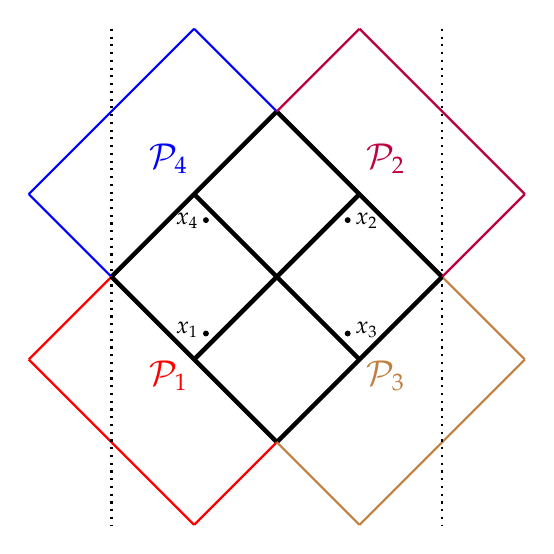
\begin{tikzpicture}[anchor=base,baseline,scale=0.6, transform shape]
		\node (opO1) at (-1.2,-1.6) [] {};
		\node (opO2) at (-1.2, 1.6) [] {};
		\node (opO3) at ( 1.2,-1.6) [] {};
		\node (opO4) at ( 1.2, 1.6) [] {};
		\node at (-1.9,-1.2) {\Large $x_1$};
		\node at (-1.9,1.1) {\Large $x_4$};
		\node at (1.9,-1.2) {\Large $x_3$};
		\node at (1.9,1.1) {\Large $x_2$};
		\node at (-1.5,-1.2) [twopt] {};
		\node at (-1.5,1.2) [twopt] {};
		\node at (1.5,-1.2) [twopt] {};
		\node at (1.5,1.2) [twopt] {};
\draw [ultra thick, black] (-1.75,-1.75)-- (1.75,1.75);
		\draw [ultra thick, black] (1.75,-1.75)-- (-1.75,1.75);
		\draw [ultra thick, black] (0,3.5) -- (-3.5,0);
		\draw [ultra thick, black] (0,-3.5) -- (-3.5,0);
		\draw [ultra thick, black] (3.5,0) -- (0,3.5);
		\draw [ultra thick, black] (3.5,0) -- (0,-3.5);
\draw [thick, blue] (0,3.5) -- (-1.75,5.25);
		\draw [thick, blue] (-5.25,1.75) -- (-1.75,5.25);
		\draw [thick, blue] (-5.25,1.75) -- (-3.5,0);
		\node at (-2.3,2.3) [blue] {\huge $\mathcal{P}_4$};
\draw [thick, red] (-3.5,0) -- (-5.25,-1.75);
		\draw [thick, red] (-5.25,-1.75) -- (-1.75,-5.25);
		\draw [thick, red] (-1.75,-5.25) -- (0,-3.5);
		\node at (-2.3,-2.3) [red] {\huge $\mathcal{P}_1$};
\draw [thick, brown] (0,-3.5) -- (1.75,-5.25);
		\draw [thick, brown] (1.75,-5.25) -- (5.25,-1.75);
		\draw [thick, brown] (5.25,-1.75) -- (3.5,0);
		\node at (2.3,-2.3) [brown] {\huge $\mathcal{P}_3$};
\draw [thick, purple] (3.5,0) -- (5.25,1.75);
		\draw [thick, purple] (5.25,1.75) -- (1.75,5.25);
		\draw [thick, purple] (1.75,5.25) -- (0,3.5);
		\node at (2.3,2.3) [purple] {\huge $\mathcal{P}_2$};
\draw [thick, black, dotted] (-3.5, 5.25) -- (-3.5,-5.25);
		\draw [thick, black, dotted] (3.5, 5.25) -- (3.5,-5.25);
	\end{tikzpicture}
	\end{center}
	\caption{The external operators at coordinates $x_i$ in their respective Poincar\'e patches $\mathcal{P}_i$. The black dotted lines are identified when the Poincar\'e patches are wrapped on the boundary of the global AdS cylinder.}
	\label{fig:Poincare_patches}	
	\end{figure}
In the new $x_i$ coordinates, the Regge limit corresponds to placing the four external points at the origin of their respective Poincar\'{e} patches,
\beq
x_1, x_2, x_3, x_4 \to 0\,.
\label{eq:regge_limit_x}
\eeq
However, $x_5$ to $x_8$ are integrated over in the CFT optical theorem.

Conformal correlators transform covariantly under the transformation \eqref{eq:xofy}.
In the scalar case we have
\beq
A\left(y_{i}\right)=(-y_{1}^{+})^{-\De_1} (y_{2}^{+})^{-\De_2} (-y_{3}^{-})^{-\De_3} (y_{4}^{-})^{-\Delta_4}  A\left(x_{i}\right)\,.
\label{eq:Ax_to_Ay}
\eeq
In the spinning case, one must additionally account for the Jacobian matrix $\partial y^a / \partial x^m$.\footnote{For external spinning operators, the conformal transformations have a non-trivial rotation matrix $\partial y^a / \partial x^m$. Conformal covariance of the correlators gives, in the representative example of two vectors and two scalars \cite{Cornalba:2009ax}, $A^{a b}\left(y_{i}\right)=\left(-y_{1}^{+} y_{2}^{+}\right)^{-1-\Delta_V}\left(-y_{3}^{-} y_{4}^{-}\right)^{-\Delta_S} \frac{\partial y_{1}^{a}}{\partial x_{1}^{m}} \frac{\partial y_{2}^{b}}{\partial x_{2}^{n}} A^{m n}\left(x_{i}\right)$. These matrices ensure that the inversion tensors are correctly mapped from $y_i$ to $x_i$ variables, preserving their form.}

Next we use conformal symmetry to express the correlator in terms of two vectors.
This is similar to expressing the correlator in terms of two scalar cross-ratios, with the difference that here we fix two, instead of the customary three, positions using translations and special conformal transformations to express the correlator in terms of the remaining two position vectors.
 We can follow \cite{Cornalba:2009ax} and use a translation to send $x_1$ to 0
which, due to the different transformations in \eqref{eq:xofy} (see also \cite{Kulaxizi:2018dxo}), will act as a special conformal transformation on the Poincar\'{e} patches for $x_3$ and $x_4$,
\beq
x_1 \to 0\,, \quad x_2 \to x_2 - x_1\,, \quad
x_{3,4} \to \frac{x_{3,4} - x_{3,4}^2 x_1}{1-2 x_{3,4} \cdot x_1 + x_{3,4}^2 x_1^2}\,.
\eeq
Next we implement a translation on the $x_3$ and $x_4$ patches (acting as special conformal transformation on $x_{1,2}$) to also map $x_4$ to 0 in its own patch and find that the correlator as a function of the Poincar\'e patch coordinates $A(x_i)$, as defined in \eqref{eq:Ax_to_Ay}, can always be expressed as
\beq
A(x_1, x_2, x_3, x_4) \approx A(0, -x, \xb/\xb^2, 0) \equiv A(x,\xb)\,,
\label{eq:Axxbar}
\eeq
with
\beq
x\approx x_1 - x_2 \,, \qquad \xb \approx x_3 - x_4\,,
\eeq
in the Regge limit \eqref{eq:regge_limit_x}.

It is further convenient to implement the coordinate change using embedding space coordinates $P^M \in \mathbb{R}^{2,d}$
\beq
P^M = \big(P^+,P^-,P^m\big)\,, \qquad P\cdot P = -P^+ P^- + \eta_{m n} P^m P^n\,.
\eeq
These are related to the coordinates $y^m \in \mathbb{R}^{1,d-1}$ of physical Minkowski space by \cite{Cornalba:2009ax}
\beq
P^M = \big(y^+, y^-, 1, y^2,y_\perp\big) \quad \Rightarrow \quad
P_{ij} \equiv -2 P_i \cdot P_j = (y_i-y_j)^2\,,
\eeq
and to the coordinates $x_i$ by
\bea
P_1^M &= -y_1^+ \left(-1,-x_1^2,x_1^m\right)\,, & & 
P_2^M =  y_2^+ \left(-1,-x_2^2,x_2^m\right)\,,\\
P_3^M &= -y_3^- \left(-x_3^2,-1, x_3^m\right), & &
P_4^M =  y_4^- \left(-x_4^2,-1, x_4^m\right)\,.
\eea{eq:xiPatches}
One can easily show that the cross-ratios \eqref{eq:crossratios} are given in terms of $x$ and $\xb$ as
\beq
z\zb = x^2 \xb^2\,, \qquad (1-z)(1-\zb) = 1 + x^2 \xb^2 + 2 x \cdot \xb\,,
\label{eq:xxb_derivation}
\eeq
and the kinematic prefactor \eqref{eq:T} becomes
\beq
T^{1234} = \frac{(-y_{1}^{+})^{-\De_1} (y_{2}^{+})^{-\De_2} (-y_{3}^{-})^{-\De_3} (y_{4}^{-})^{-\Delta_4}}{x^{\De_1 + \De_2} \xb^{\De_3 + \De_4}}\,.
\eeq
When combining \eqref{eq:OPE_s} and \eqref{eq:Ax_to_Ay}, the numerator of the last expression cancels the Jacobian prefactor in \eqref{eq:Ax_to_Ay} to give,
\beq
A\left(x_{i}\right) = \frac{A^{1234}(z, \zb)}{x^{\De_1 + \De_2} \xb^{\De_3 + \De_4}}\,.
\label{eq:strip_A}
\eeq
 If we now study the correlator $A^{3652}(x_i)$, a priori we have to take into account that only $x_2$ and $x_3$ are affected by the Regge limit. However, we will assume that the integration will be dominated by the region where the integration points are also boosted. Using the embedding space coordinates
\bea
P_5^M =  -y_5^+ \left(-1,-x_5^2,x_5^m\right)\,, \qquad
P_6^M &= y_6^- \left(-x_6^2,-1, x_6^m\right)\,,
\eea{eq:x56Patches}
we find
\beq
x' \approx x_5 - x_2 \,, \qquad \xb' \approx x_3 - x_6\,.
\eeq
Where the primed variables are meant to emphasize that the points $1,4$ are replaced by $5,6$ in this correlator as compared to \eqref{eq:Axxbar}.
Performing these steps for all the correlators in \eqref{eq:cft_optical_theorem_s} we find,
\bea
\dDisc_t A_{\text{1-loop}}(x_{12},x_{34}) = -\frac{1}{2}
\sum\limits_{\cO_5, \cO_6}  \int dx_5 dx_6 \, \Disc_{23} A^{3652}_{\text{tree}}(x_{36},x_{52})   \\
									\bS_5 \bS_6	\Disc_{14} A^{1564}_{\text{tree}}(x_{15},x_{64}) \Big|_{\left[\cO_5\cO_6\right]}\,,
\eea{eq:cft_optical_theorem_x}
where we stop explicitly mentioning that we are dealing with only the contribution of double-trace operators as single-trace contributions are subleading in the limit considered.
Let us stress that in order to write the correlators on the right hand side in terms of two differences, we assumed that each of the individual tree-level correlators are in the Regge limit themselves. 
The easiest way to justify this is in Fourier space using the impact parameter transform defined below.
Each tree-level position space correlator is dominated by a power $\sigma^{1-j(\nu)}$ in the Regge limit, which maps to a power of the AdS center of mass energy $S^{j(\nu)-1}$ in impact parameter space. Since the optical theorem is multiplicative in impact parameter space, subleading Regge trajectories or kinematical corrections from the conformal block at finite boost get mapped to smaller powers of $S$, and therefore do not contribute to the leading behavior.
The eikonal approximation in AdS \cite{Cornalba:2007zb} gives additional intuition for this, since it means that even in AdS, the particles remain essentially undeflected, scattering forward each time they exchange a Pomeron. Furthermore, we will show in section \ref{sec:Appendix_tchannel} that this configuration reproduces the behavior at one-loop derived in \cite{Meltzer:2019pyl}.

\subsection{Impact parameter space}
\label{sec:impact}





Let us now consider the two-point functions $\<\tl \cO_5 \tl \cO_7\>$ and $\<\tl \cO_8 \tl \cO_6\>$ for the shadow transforms in \eqref{eq:cft_optical_theorem_x}.
In the Regge configuration, $x_5$ is the patch of $x_1$, $x_6$ is the patch of $x_4$, $x_7$ is the patch of $x_2$ and $x_8$ is the patch of $x_3$.
As explained in \cite{Cornalba:2007zb,Kravchuk:2018htv}, the two-point function between two coordinates on adjacent Poincar\'e patches has an additional phase factor $e^{i \pi \Delta}$ and this phase can be accounted for by switching from the $i\e$ prescription of a Feynman propagator to that of a Wightman propagator (see \cite{Cornalba:2007zb}).
The normalization of the shadow transform in \eqref{eq:shadowtransform} and \eqref{eq:shadownormali} is obtained from the Fourier transform of a two-point function as the shadow transform acts multiplicatively in Fourier space (see section 3.2 of \cite{Karateev:2018oml}). The normalization in \eqref{eq:shadownormali} is obtained from the Fourier transform of a Euclidean two-point function, which matches the one of a Lorentzian two-point function with Feynman $i\e$ prescription. The Wightman propagator in momentum space however has support only on the future lightcone and the coefficient of the Fourier transform is different (see Appendix B of \cite{Cornalba:2007zb} and 
section 2.1 of \cite{Gillioz:2018mto})
\bea
\int dx \frac{e^{-2iq\cdot x}}{\left[-(x^{0}-i\epsilon)^{2} + \vec{x}^{2}\right]^{\De}} =\cM_{\cO} 
 \,\Theta(q^{0}) \,\Theta(-q^{2})\left(-q^{2}\right)^{\De-\frac{d}{2}}\,,
\eea{eq:WightmanFT}
with 
\begin{equation}
 \cM_{\cO}  = \frac{2\pi^{\frac{d}{2}+1}}{\Gamma(\De)\Gamma\big(\De - \frac{d}{2} + 1\big)} \,.
\end{equation}
Consequently we change the normalization $N_\cO$ of the shadow transform in \eqref{eq:shadowtransform} to (for scalar operators)
\be
\mathcal{N}_\cO = \cM_\cO \cM_{\tl \cO}  \,. 
\label{eq:new_normali}
\ee

Next we define, following \cite{Cornalba:2007fs}, the impact parameter representation as the Fourier transform of the discontinuity of the correlator in the two remaining vectors\footnote{The AdS impact parameter representation was previously defined in \cite{Cornalba:2007fs,Cornalba:2006xm,Cornalba:2008qf} as the Fourier transform of the correlator on the second sheet $A(z,\zb^\circlearrowleft)$. Since this contribution dominates in the Regge limit, it is indistinguishable from the discontinuity of the correlator in this limit.
However, in the $t$-channel the two notions are clearly different and it was necessary to take the discontinuity to derive \eqref{eq:cft_optical_theorem_intro}.
In the next section we will see that the discontinuity is the better choice also in the $s$-channel.}
\beq
\Disc_{14} A^{1jk4}(x_{1j},x_{k4}) = \int dp \, d\bar{p} \, e^{-2i p \cdot x_{1j}-2i \bar{p} \cdot x_{k4}} B^{1jk4}(p,\bar{p})\,,
\label{eq:BtoA}
\eeq
where the function $B(p,\bar{p})$ has support only on the future Milne wedge of $p$ and $\bar{p}$.
Using \eqref{eq:disc_relation56} on \eqref{eq:BtoA} we get the Fourier transform of $\Disc_{23}$.
\be
\label{eq:BtoA23}
\Disc_{23} A^{3kj2}(x_{3k},x_{j2}) = -\int dp \, d\bar{p} \, e^{-2i p \cdot x_{3k}-2i \bar{p} \cdot x_{j2}} B^{3kj2}(-p,-\bar{p})^{*}\,.
\ee
The causal relations and thus the $i\epsilon$ prescription in \eqref{eq:BtoA23} are opposite to those in \eqref{eq:BtoA} and the complex conjugation prescribed in \eqref{eq:disc_relation56} compensates for that.
Inserting \eqref{eq:BtoA} into \eqref{eq:cft_optical_theorem_x} and using that $A^{1\tilde{5}\tilde{6}4}_{\text{tree}}$ is a double shadow transform of $A^{1784}_{\text{tree}}$ we obtain, upon using \eqref{eq:disc_relation56} for the $\Disc_{23}$,
\bea
{}& \dDisc_t A_{\text{1-loop}}(x_{12},x_{34})  = \frac{1}{2}
\sum\limits_{\cO_5, \cO_6}  \int dx_{5}\, dx_{6}\, dx_{7}\, dx_{8}\; 	\int dp \, d\pb \,  dp' \, d\bar{p}' 	  \\ 
& \qquad 
	\times  e^{-2i (p' \cdot x_{36}+ \bar{p}' \cdot x_{52}+ p \cdot x_{17}+ \bar{p} \cdot x_{84})} B^{3652}_\text{tree} (-p',-\pb')^* B^{1564}_\text{tree}(p,\pb)  \\
&\qquad	
\times \frac{T^{(\rho_5)}(x_{75})}{\mathcal{N}_{\cO_{5}}\left[-(x^{0}_{75}-i\epsilon)^{2} + \vec{x}_{75}^{2}\right]^{d-\De_5}}  \frac{T^{(\rho_6)}(x_{68})}{\mathcal{N}_{\cO_{6}}\left[-(x^{0}_{68}-i\epsilon)^{2} + \vec{x}_{68}^{2}\right]^{d-\De_6}} \Bigg|_{\left[\cO_5\cO_6\right]} \,.
\eea{eq:ftgluing1}
$T^{(\rho)}(x_{ij})$ is the tensor structure for the two-point function of an operator with $SO(d)$ quantum number $\rho$. For example it is the familiar inversion tensor $\eta^{\mu\nu}-2\frac{x^{\mu}x^{\nu}}{x^{2}}$ for spin 1 operators. Note that we have $B^{1564}_\text{tree}$ instead of $B^{1784}_\text{tree}$, as the superscripts now only indicate the dimensions of the corresponding operators and $\Delta_5 = \De_7$, $\De_6 = \De_8$.

We can now express the two-point functions from the shadow transforms in Fourier space by inverting \eqref{eq:WightmanFT}
\be
\label{eq:shadow2ptFT}
\frac{T^{(\rho)}(x)}{\left[-(x^{0}-i\epsilon)^{2} + \vec{x}^{2}\right]^{d-\De}}  ={} \frac{\mathcal{M}_{\tl\cO}}{\pi^{d}}\int\limits_{M} dq\, e^{-2iq\cdot x}\, \widehat{T}^{(\rho)}(q) \, (-q^{2})^{\frac{d}{2}-\De} \,.
\ee
The Fourier space integral is over the future Milne wedge $M$ as the Fourier transform has support only on this domain.
$\widehat{T}^{(\rho)}(q)$ is the tensor structure of the two-point function in Fourier space,
which has been discussed for example in \cite{Gillioz:2018mto}.
It is a tensor composed of $q^\mu$ and $\eta^{\mu \nu}$ that can be factorized into a product of new tensors $t^{(\rho)}(q)$ as follows
\beq
\widehat{T}^{(\rho)}(q)^{\mu_1 \ldots \mu_{|\rho|}}_{\nu_1 \ldots \nu_{|\rho|}}
= t^{(\rho)}(q)^{\mu_1 \ldots \mu_{|\rho|}}_{\sigma_1 \ldots \sigma_{|\rho|}}
t^{(\rho)}(q)^{\sigma_1 \ldots \sigma_{|\rho|}}_{\nu_1 \ldots \nu_{|\rho|}}\,.
\label{eq:T_factorization}
\eeq
Using \eqref{eq:shadow2ptFT} in \eqref{eq:ftgluing1} we end up with four position integrals over $x_{5},x_{6},x_{7},x_{8}$ and six  integrals over $q,\bar{q}$ (from the four-point functions) and $p,\bar{p},p',\bar{p}'$. The four position integrals give  four Dirac delta functions with which we can eliminate the $q,\bar{q},p',\bar{p}'$ integrals to obtain
\bea
\dDisc_t A_{\text{1-loop}}(x_{12},x_{34})		= \ &
\frac{\pi^{2d}}{2}
\sum\limits_{\cO_5, \cO_6}  \frac{1}{\cM_{\cO_5}\cM_{\cO_6}}   \int dp \, d\pb\,
		e^{-2i (p \cdot x_{12}+ \pb \cdot x_{34})}      \\
&	\frac{B^{3652}_\text{tree}(-\pb,-p)^* \;\,  \widehat{T}^{(\rho_5)}(p) \,  \widehat{T}^{(\rho_6)}(\bar{p}) \;\, B^{1564}_\text{tree}(p,\pb)}{(-p^{2})^{\De_5-\frac{d}{2}}(-\bar{p}^{2})^{\De_6-\frac{d}{2}}} \Bigg|_{\left[\cO_5\cO_6\right]} \,,
\eea{eq:circ_impact1}
with an implicit index contraction between $B^{1564}_\text{tree}$ and $B^{3652}_\text{tree}$ and the tensor structures $\widehat{T}^{(\rho)}$.
At this point we use \eqref{eq:T_factorization} and absorb the $ t^{(\rho)}(q)$ tensors into the definition of the phase shifts $B_\text{tree}$. This means that one needs to take it into account if one wants to relate tensor structures of CFT correlators and phase shifts, but we will not need to do such a basis change explicitly in this work.
Using \eqref{eq:discs_Regge} we see that the double discontinuity corresponds to the quantity
$- \Re B(p,\bar{p})$
in impact parameter space.
Thus we find the following gluing formula for the impact parameter representation, which is purely multiplicative,
\beq
- \Re B_{\text{1-loop}}(p,\bar{p}) = \frac{\pi^{2d}}{2}
\sum\limits_{\cO_5, \cO_6}  \frac{1}{\cM_{\cO_5}\cM_{\cO_6}} \, 
\frac{B^{3652}_\text{tree}(-\pb,-p)^* \,  B^{1564}_\text{tree}(p,\pb)}{(-p^{2})^{\De_5-\frac{d}{2}}(-\bar{p}^{2})^{\De_6-\frac{d}{2}}}  \Big|_{\left[\cO_5\cO_6\right]} \,.
\label{eq:gluing_B}
\eeq
Let us consider the case when $\cO_5 = \cO_1$ and $\cO_6 = \cO_3$. In this case, it is useful to strip out a scale factor similar to that in \eqref{eq:strip_A} from the impact parameter representation
\beq
B^{jjkk}(p, \bar{p})=\frac{\cM_{\cO_j} \cM_{\cO_k} \; \mathcal{B}^{jjkk}(p,\pb)}{\left(-p^{2}\right)^{\frac{d}{2}-\Delta_{j}}\left(-\bar{p}^{2}\right)^{\frac{d}{2}-\Delta_{k}}}     \, .
\label{eq:strip_pairwise}      
\eeq
Using \eqref{eq:WightmanFT} one sees that with this choice of normalization the impact parameter representation of the MFT correlator is $\mathcal{B}^{jjkk}_{\text{MFT}}=1$,
which is necessary for the eikonalization of the  phase shift in AdS gravity.
Inspired by this fact we choose the normalization
\beq
B^{ijkl}(p, \bar{p})=\frac{\sqrt{\cM_{\cO_i} \cM_{\cO_j} \cM_{\cO_k} \cM_{\cO_l}} \; \mathcal{B}^{ijkl}(p,\pb)}{\left(-p^{2}\right)^{\frac{d-\Delta_{i}-\Delta_{j}}{2}}\left(-\bar{p}^{2}\right)^{\frac{d-\Delta_{k}-\Delta_{l}}{2}}}     \, ,
\label{eq:strip}      
\eeq
for the general case.
This gives  the following compact form for the optical theorem in impact parameter space
\bea
- \Re \cB_{\text{1-loop}}(p,\bar{p}) =  \frac{1}{2}
\sum\limits_{\cO_5, \cO_6}    \; \cB^{3652}_\text{tree}(-\pb,-p)^* \; \cB^{1564}_\text{tree}(p,\pb)  \; \Bigg|_{\left[\cO_5\cO_6\right]}  \,.
\eea{eq:gluing_stripped}

We also introduce impact parameter variables later.
\beq
S= \sqrt{p^2 \pb^2}, \qquad \cosh L=-\frac{p \cdot \bar{p}}{\sqrt{p^2 \pb^2}}\,.    \label{eq:impactCR1}
\eeq
In \cite{Meltzer:2019pyl}, the Regge limit of a one-loop four-point function of scalars was studied in the large $\lambda$ regime with $S\gg \lambda\gg 1$. The contribution of tidal excitations to the correlator is suppressed in this regime. It corresponds to just one term in the sum on the right hand side of \eqref{eq:gluing_stripped} i.e.\ with $\cO_5 = \cO_1$ and $\cO_6 = \cO_3$. We show in section \ref{sec:Dav_match} that this term from our formula \eqref{eq:gluing_stripped} reproduces the result from \cite{Meltzer:2019pyl} in the large $\lambda$ or equivalently the large $\De_{\text{gap}}^{2}$ limit. We do not need to discard any shadow double-trace contributions for this match. This motivates us to assume that the only non-zero contributions to the gluing of tree-level correlators in the Regge limit is from the physical double-traces $[\cO_5 \cO_6]$, and we will drop the explicit projections henceforth. This is compatible with the intuition that there is no need to project out shadow operators in a Lorentzian CFT optical theorem.



\subsection{$s$-channel discontinuities in the Regge limit}
\label{sec:sdisc}


Next we have to analyze the discontinuities on the right hand side of  the optical theorem \eqref{eq:cft_optical_theorem_s}. The discontinuity of the scalar $s$-channel block was recently computed in general without taking the Regge limit in \cite{Caron-Huot:2020nem} and we will review it here. The generalization to external spinning operators is done in section \ref{sec:vertex_function}, after taking the Regge limit. Let us take the conformal partial wave expansion \eqref{eq:partialwaveexpansion} in the $s$ channel and use the symmetry of the integrand to extend the integration region at the cost of a factor $1/2$
\be
A^{1234}(z,\zb) &= \frac{1}{2} \sum_{J} \int_{\frac d 2 - i \oo}^{\frac d 2 + i\oo} \frac{d\De}{2\pi i}\,
I^{1234}(\De,J)\, \psi^{1234}_{\text{good},\cO} (z,\zb) \,.
\label{eq:partialwaveexpansion_s}
\ee
Let
$\psi^{1234}(z,\zb)$ be the partial wave $\Psi^{1234}(y_i)$ with the prefactor $T^{1234}$ stripped off. $\psi^{1234}_{\text{good},\cO} (z,\zb)$ is the conformal partial wave with an additional term that
vanishes for integer spin but ensures favorable properties for non-integer spin  \cite{Caron-Huot:2020nem}. The new partial wave is given by
\bea
\psi^{1234}_{\text{good},\cO}(z,\zb)  =  \psi^{1234}_\cO(z,\zb)   +  2\pi \, S(\cO_3 \cO_4 [\tl\cO^\dag]) \, K_{J+d-1,1-\Delta} \, \xi_{\De,J}^{(a,b)} \, g^{1234}_{J+d-1,1 - \Delta}(z,\zb) \,,
\label{eq:psigood}\end{aligned}\end{equation}
where $g^{1234}_{\De,J}(z,\zb)$ is the usual conformal block, the constants $a,b$ are defined below \eqref{eq:dDisc_conventional} and
\bea
\xi_{\De,J}^{(a,b)} = & \left(s^{(a,b)}_{\Delta+J}-s^{(a,b)}_{\Delta+2-d-J}\right) \frac{\Gamma\big(-J-\tfrac{d-2}{2}\big)}{\Gamma(-J)}   \,, \\
s^{(a,b)}_{\beta} = &  \, \frac{\sin\big(\pi(a+\beta/2 )\big) \, \sin\big(\pi(b+\beta/2)\big)}{\sin(\pi\beta)}  \,, \\
K_{\De,J} = &\, \frac{\Gamma(\De - 1)}{\Gamma\big(\De - \frac{d}{2}\big)}\, \kappa^{(a,b)}_{\De+J}  \,,\\
\kappa^{(a,b)}_{\beta} = &\, \frac{\Gamma\big(\frac{\beta}{2}-a\big)\Gamma\big(\frac{\beta}{2}+a\big)\Gamma\big(\frac{\beta}{2}-b\big)\Gamma\big(\frac{\beta}{2}+b\big)}{2\pi^{2}\Gamma(\beta-1)\Gamma(\beta)}  \,.
\label{eq:shortening}\end{aligned}\end{equation}
With this conformal partial wave it is possible to compute the discontinuity exactly \cite{Caron-Huot:2020nem}
\beq
\frac{\Disc_{14} \, \psi^{1234}_{\text{good},\cO}(z,\zb)}{S(\cO_3 \cO_4 [\tl\cO^\dag])} = \frac{R^{1234}_{\cO}(z,\zb)}{\pi i \kappa_{\De,J}^{(a,b)}}\,.
\label{eq:Disc14Psi}
\eeq
Here $R$ is the so-called Regge block
\bea
R^{1234}_{\cO}(z,\zb) &= g^{1234}_{1-J,1-\Delta}
-\kappa'^{(a,b)}_{\Delta+J} g^{1234}_{\Delta,J}
-\frac{\Gamma(d-\Delta-1)\Gamma\big(\Delta-\tfrac{d}{2}\big)}{\Gamma(\Delta-1)\Gamma\big(\tfrac{d}{2}-\Delta\big)}\,\kappa'^{(a,b)}_{d-\Delta+J}\ g^{1234}_{d-\Delta,J}+
\\ &\phantom{=}+
\frac{\Gamma(J+d-2)\Gamma\big(-J-\tfrac{d-2}{2}\big)}{\Gamma\big(J+\tfrac{d-2}{2}\big)\Gamma(-J)}
\,\kappa'^{(a,b)}_{\Delta+J}\ \kappa'^{(a,b)}_{d-\Delta+J}\ g^{1234}_{J+d-1,1-\Delta}\,,
\label{eq:Regge_block}\end{aligned}\end{equation}
with $\kappa'^{(a,b)}_{\beta}$ defined as
\be
\label{eq:kappaprime}
\kappa'^{(a,b)}_{\beta} = \frac{r^{(a,b)}_{\beta}}{r^{(a,b)}_{2-\beta}}\,,
\qquad
r^{(a,b)}_{\beta} = \frac{\Gamma(\frac{\beta}{2}+a)\Gamma(\frac{\beta}{2}+b)}{\Gamma(\beta)}    \, .
\ee
$\Disc_{23}$ in the $3412$ OPE channel can be obtained by using \eqref{eq:disc_relation} on \eqref{eq:Disc14Psi}
\beq
\frac{\Disc_{23} \, \psi^{3412}_{\text{good},\cO}(z,\zb)}{S(\cO_{1}\cO_{2}[\tl\cO^\dag])}= \frac{R^{3412}_{\cO}(z,\zb)}{\pi i \kappa_{\De,J}^{(-b,-a)}}\,,
\eeq
which was the reason to consider this channel for the correlators on the right hand side of \eqref{eq:cft_optical_theorem_s}.
The Regge block is dominated in the Regge limit by \cite{Caron-Huot:2020nem,Caron-Huot:2017vep,Cornalba:2007fs}
\beq
g^{1234}_{1-J,1-\De}(z,\zb) = \frac{4 \pi^{\frac{d}{2}} \Gamma(\De-\frac{d}{2})}{\Gamma(\De-1)} \sigma^{1-J} \left( \Omega_{\De-\frac{d}{2}}(\rho)
+ O(\sigma) \right)\,.
\eeq
The $\sigma,\rho$ cross-ratios introduced here are defined as
\beq
\sigma = \sqrt{z \zb} = \sqrt{x^2 \xb^2}\,, \quad
\cosh(\rho) = \frac{z+\zb}{2 \sqrt{z \zb}} = -\frac{x \cdot \bar{x}}{\sqrt{x^2 \xb^2}} \,.
\label{eq:sigma_rho}
\eeq
$\Omega_{i\nu}(\rho)$ is the harmonic function on $d-1$ dimensional hyperbolic space $H_{d-1}$ transverse to the scattering plane in $\text{AdS}_{d+1}$ \cite{Cornalba:2006xk}
\bea
\Omega_{i \nu} (\rho)
={}&-\frac{i \nu \sin(\pi i \nu) \Gamma(h-1+i \nu) \Gamma(h-1-i \nu) }{2^{2h-1}\pi^{h+\frac{1}{2}} \Gamma\big(h-\frac{1}{2}\big)} \\
& {}_2F_1 \left(h-1+i \nu, h-1-i\nu,h-\frac{1}{2},\frac{1-\cosh(\rho)}{2}\right)\,.
\label{eq:Omega}\end{aligned}\end{equation}
Inserting everything into \eqref{eq:partialwaveexpansion_s}, we find the following expression for the discontinuity of the correlator in the Regge limit
\beq
\label{eq:sameoldregge}
\Disc_{14}  A^{1234}(z,\bar{z}) = 2\pi i\sum\limits_J \int\limits_{-\oo}^{\oo} d\nu \ \a(\nu,J)\, \sigma^{1-J} \Omega_{i\nu} (\rho)\,,
\eeq
with
\beq
\label{eq:alphaus}
\a(\nu,J) = - \, \frac{\pi^{\frac d 2 -2} \, S\big(\cO_{3}\cO_{4}\big[\big(-i\nu-\frac{d}{2}\big)^\dag\big]\big) \, \Gamma(i \nu)}{2\pi \kappa_{i\nu+\frac{d}{2},J}^{(a,b)}\, \Gamma\big(i \nu + \frac d 2 -1\big)} \,I^{1234}\!\left(i \nu + \frac{d}{2},J\right) .
\eeq

As in flat space the sum in \eqref{eq:sameoldregge} is dominated by the large $J$ contributions in the Regge limit and only finite due to a conspiration of the coefficients to ensure Regge boundedness.
The next step is therefore to perform a  Sommerfeld-Watson resummation over $J$ to evaluate \eqref{eq:sameoldregge}. Also, note that the spectral function, as given by the Lorentzian inversion formula \cite{Caron-Huot:2017vep}, is of the form
\be
I^{1234}(\nu) = I^{1234,t}(\nu) + (-1)^{J}I^{1234,u}(\nu)   \,.        \label{eq:spectral_break}
\ee
Let us first consider the case of a correlator with pairwise equal external operators i.e.\ $a=b=0$, $I^{1234,t} = I^{1234,u}$, where only even spins are exchanged.
Now for the resummation we replace the sum by an integral,
\beq
2\sum\limits_{J \text{ even}} \to
\int_C dJ \frac{e^{i\pi J}}{1-e^{i\pi J}}  \,.
\label{eq:sommerfeld-watson}
\eeq
The contour $C$ encloses all poles on the positive real axis (at even integers) in a clockwise direction.
The leading Regge trajectory is given by the operators with the lowest dimension $\De(J)$ for every even spin $J$ and $\a(\nu,J)$ has poles at $i \nu = \pm (\De(J)- d/2)$.
Defining the inverse function $j=j(\nu)$ of the spectral function $\De(J)$ by
\beq
\nu^2 + \big(\De(j(\nu))-\tfrac{d}{2}\big)^2 = 0\,,
\eeq
we see that the poles in $\nu$ translate into a single pole at $J=j(\nu)$.
By deforming the $J$ contour to the left one sees that the $J$ integral is given by the residue at $J=j(\nu)$, i.e.
\begin{equation}
    \Disc_{14}  A^{1234}(z,\bar{z}) = 2\pi i \int\limits_{-\oo}^{\oo} d\nu \ \a(\nu)\, \sigma^{1-j(\nu)} \Omega_{i\nu} (\rho)\,,
    \label{eq:discA_regge}
\end{equation}
where
\begin{equation}
    \a(\nu)  = - \underset{J=j(\nu)}{\Res} i \, \frac{e^{i\pi J}}{1-e^{-i\pi J}} \frac{\pi^{\frac d 2 -2} \, S\big(\cO_{3}\cO_{4}\big[\big(-i\nu-\frac{d}{2}\big)^\dag\big]\big) \, \Gamma(i \nu)}{\kappa_{i\nu+\frac{d}{2},J}^{(a,b)}\, \Gamma\!\big(i \nu + \frac d 2 -1\big)} \,
    I^{1234,t}\left(i \nu + \frac{d}{2},J\right) .
\end{equation}
When the operators are not pairwise equal, the even and odd spin operators organize into two analytic families as evident from the Lorentzian inversion formula \cite{Caron-Huot:2017vep}. To obtain the contribution of the leading Regge trajectory we still sum over the even spin exchanges. The result is of the same form as in \eqref{eq:discA_regge} with $I^{1234,t}$ replaced by $ \frac{1}{2}I^{1234}$ in $\alpha(\nu)$.
For the other correlator we can use \eqref{eq:disc_relation} to see that we get an analogous result with the complex conjugate spectral function
\beq
\Disc_{23} A^{3412}(z,\bar{z}) = 2\pi i \int\limits_{-\oo}^{\oo} d\nu \ \a(\nu)^*\, \sigma^{1-j(\nu)} \Omega_{i\nu} (\rho)\,.
\eeq
One can show that the corresponding impact parameter representation is given in general
by the same spectral function times a multiplicative factor which cancels poles for the external double-trace operators \cite{Cornalba:2006xm}
\beq
\cB(p,\pb) = 2\pi i \int\limits_{-\oo}^{\oo} d\nu \ \b(\nu)\, S^{j(\nu)-1} \Omega_{i\nu} (L)\,,
\label{eq:B}
\eeq
where
\beq
\label{eq:betaexpr}
\b(\nu) = \frac{ 4 \pi^{2-d}(\sqrt{\cM_{\cO_1} \cM_{\cO_2} \cM_{\cO_3} \cM_{\cO_4}})^{-1} \; \a(\nu)}
{\chi_{j(\nu)}(\nu)  \,\chi_{j(\nu)}(-\nu) }\,,
\eeq
with the definition
\begin{equation}
    \chi_{j(\nu)}(\nu) = \Gamma\left( \frac{\Delta_1+\Delta_2+j(\nu)-d/2 + i \nu}{2}\right)
    \Gamma\left( \frac{\Delta_3+\Delta_4+j(\nu)-d/2 + i \nu}{2}\right).
    \label{eq:chi_definition}
\end{equation}
The impact parameter space cross-ratios, analogous to \eqref{eq:sigma_rho}, are
\beq
S= \sqrt{p^2 \pb^2}, \qquad \cosh L=-\frac{p \cdot \bar{p}}{\sqrt{p^2 \pb^2}}\,.    \label{eq:impactCR}
\eeq
In the dual AdS scattering process  these cross ratios are interpreted  as the squared of the energy with respect to global time and as
the impact parameter in the transverse space $H_{d-1}$.



\subsection{Spinning particles and the vertex function}
\label{sec:vertex_function}


In this section we will introduce concrete expressions for the tree amplitudes with spinning external legs and show that the contributions of the contracted spinning legs can be expressed in terms of a scalar function of three spectral parameters which we call the vertex function, analogous to \eqref{eq:V_flat_def} in flat space.
We construct tensor structures in terms of differential operators, which are a Regge limit version of weight-shifting operators that generate spinning conformal blocks from the scalar ones \cite{Costa:2011dw,Karateev:2017jgd}.
It is convenient to work with tensor structures which are homogeneous in $p$ and $\bar{p}$, i.e.\ independent of the cross-ratio $S$ in \eqref{eq:impactCR}, such that all tensor structures have the same large $S$ behavior in the Regge limit. These differential operators can be constructed from the covariant derivative on the hyperboloid $H_{d-1}$ and from $\hat{p}= p/|p|, \hat{\bar{p}}=\bar{p}/|\bar{p}|$
\cite{Cornalba:2009ax,Costa:2017twz}.
The possible differential operators that generate spin for a single particle are
\beq
\mathcal{D}^{\rho,k}_{\mathbf{m}} (p) =
\hat{p}_{m_1} \ldots \hat{p}_{m_k} {\nabla_{p}}_{m_{k+1}} \ldots {\nabla_{p}}_{m_{|\rho|}} \,, \qquad k = 0,\ldots, |\rho|\,.
\label{eq:ts_operators}
\eeq
Tree diagrams for exchange of the Pomeron   then have the form
\beq
\cB^{(\De_5,\rho_5),(\De_6,\rho_6)}_{\mathbf{m} \mathbf{n}}  (p,\bar{p})
= 2\pi i\int\limits_{-\infty}^\infty d\nu \, S^{j(\nu)-1}
\mathfrak{D}^{(\De_5,\rho_5),(\De_6,\rho_6)}_{\mathbf{m} \mathbf{n}} (\nu)\,
\Omega_{i \nu} (L)\,.
\label{eq:Btree_differential}
\eeq
Here
$\cB^{(\De_5,\rho_5),(\De_6,\rho_6)}_{\mathbf{m}\mathbf{n}}  (p,\bar{p})$ is defined just as in \eqref{eq:BtoA} and \eqref{eq:strip}, but with tensor structures constructed from $\hat{p}$ and $\hat{\bar{p}}$.
In \eqref{eq:Btree_differential} we introduced the following definition for the combination of spectral functions $\b(\nu)$ and differential operators that generate different tensor structures
\beq
\mathfrak{D}^{(\De_5,\rho_5),(\De_6,\rho_6)}_{\mathbf{m} \mathbf{n}} (\nu)
= \sum\limits_{k_5=0}^{|\rho_5|}  \sum\limits_{k_6=0}^{|\rho_6|} \beta^{k_5,k_6}_{(\De_5,\rho_5),(\De_6,\rho_6)} (\nu)
\mathcal{D}^{\rho_5,k_5}_{\mathbf{m}} (p) \mathcal{D}^{\rho_6,k_6}_{\mathbf{n}} (\bar{p})\,.
\label{eq:Dfrak}
\eeq
Notice that, in contrast to flat space, we do not impose a full factorization into three-point structures but rather allow for a separate spectral function for each combination of three-point structures.

The next step is to derive the general functional form of \eqref{eq:gluing_stripped} after the contractions and sums have been done. We begin by inserting \eqref{eq:Btree_differential} into \eqref{eq:gluing_stripped},
\begin{align}
    - \Re \cB_{\text{1-loop}} (p,\pb)={} & 2\pi^{2}  \sum\limits_{\De_5,\De_6,\rho_5,\rho_6} \int\limits_{-\infty}^\infty d\nu_1 d\nu_2 \, S^{j(\nu_1) + j(\nu_2)-2}
    \label{eq:Btilde_neater_fs}                                                                                                                                      \\
                                         & \mathfrak{D}^{(\De_5,\rho_5),(\De_6,\rho_6)}_{\mathbf{m} \mathbf{n}} (\nu_1)^*\, \Omega_{i \nu_1} (L)
    \,\pi_{\rho_{5}}^{\mathbf{m}; \mathbf{p}}
    \pi_{\rho_{6}}^{\mathbf{n}; \mathbf{q}}
    \,\mathfrak{D}^{(\De_5,\rho_5),(\De_6,\rho_6)}_{\mathbf{p} \mathbf{q}} (\nu_2)
    \,\Omega_{i \nu_2} (L)\,.
    \nonumber
\end{align}
Here $\pi_\rho$ is the projector to the irreducible representation $\rho$ of $SO(d)$, which is necessary because the operators \eqref{eq:ts_operators} do not ensure the properties of irreducible representations such as tracelessness and Young symmetrization.
Next we will show how one can replace the contractions and derivatives in the previous equation by spectral parameters.
Note first that due to $p \cdot \nabla_p = 0$, all contractions involving $\hat{p}$ or $\hat{\pb}$ give factors of their norm $-1$. The remaining contractions involve only covariant derivatives. These contracted derivatives can all be replaced by functions of the spectral parameters by using the Laplace equation for the harmonic function
\beq
\left( \nabla_{H_{d-1}}^2 + \nu^2 + (d/2-1)^2 \right) \Omega_{i \nu} (L) = 0 \,.
\label{eq:nabla}
\eeq
Using this equation, factors of $\nabla_p^2$ can directly be replaced.
To evaluate contractions between derivatives acting on different harmonic functions we expand the product of two scalar harmonic functions as follows,
\beq
\Omega_{i \nu_1} (L) \Omega_{i \nu_2} (L) = \int\limits_{-\infty}^\infty d\nu \, \Phi(\nu_1,\nu_2,\nu) \Omega_{i \nu} (L)\,,
\label{eq:Omega_prod}
\eeq
where $\Phi(\nu_1,\nu_2,\nu)$ was computed (for the similar case of harmonic functions on AdS$_{d+1}$) in appendix D of \cite{Penedones:2010ue}.\footnote{Note that $\Phi_{\text{here}} \Omega_{i \nu}(0)=\Phi_{\text{there}}$.}
By acting repeatedly with \eqref{eq:nabla} on this equation, one can determine the function $W_k$ that appears in
\beq
{\nabla_{p}}_{m_1} \ldots {\nabla_{p}}_{m_k}   \Omega_{i \nu_1} (L)
\nabla_p^{m_1} \ldots \nabla_p^{m_k} \Omega_{i \nu_2} (L) =
\int\limits_{-\infty}^\infty d\nu \, W_{k} \big(\nu_1^2,\nu_2^2,\nu^2\big)\, \Phi(\nu_1,\nu_2,\nu) \,\Omega_{i \nu} (L)\,.
\label{eq:Wk}
\eeq
$W_{k}$ is a fixed kinematical  polynomial of maximal degree $k$ in its arguments.
For example, the first non-trivial case is
\beq
\int\limits_{-\infty}^\infty \!\! d\nu \, \Phi(\nu_1,\nu_2,\nu) \nu^2 \,\Omega_{i \nu} (L)
= \left( \nu_1^2 + \nu_2^2 +(\tfrac{d}{2}-1)^2 \right) \Omega_{i \nu_1} (L)\, \Omega_{i \nu_2} (L)
-2 \nabla_\mu \Omega_{i \nu_1} (L) \nabla^\mu \Omega_{i \nu_2} (L),
\eeq
from which one can read off $W_{0}$ and $W_1$ to be
\beq
W_{0} \big(\nu_1^2,\nu_2^2,\nu^2\big) = 1\,, \qquad
W_{1} \big(\nu_1^2,\nu_2^2,\nu^2\big)  = \frac{1}{2} \Big(
\nu_1^2 + \nu_2^2 - \nu^2 + (d/2-1)^2
\Big) .
\eeq
More generally, by acting with the Laplacian on both sides of (\ref{eq:Wk}) one can derive a recursion relation of the form
\bea
{}&		\int d\nu \,W_{k+1}(\nu_i) \, \Phi(\nu_i)\, \Omega_{i \nu} (L) = \int d\nu \,W_{k}(\nu_i)\,W_{1}(\nu_i)\,\Phi(\nu_i) \,\Omega_{i \nu} (L) \\
& + \frac{1}{2} \left([\nabla^2,\nabla_{m_1}\dots\nabla_{m_{k}}] \Omega_{i \nu_1} (L) \nabla^{m_1}\dots\nabla^{m_{k}} \Omega_{i \nu_2} (L) +(\nu_1 \leftrightarrow \nu_2)\right) \,.
\label{eq:Wrecrer}\end{aligned}\end{equation}
The terms with commutators, which will vanish in the flat space limit, can be evaluated using the fact that the commutators of covariant derivatives can be replaced by Riemann tensors, which for the hyperboloid can be written in terms of the metric. This means that these terms have two derivatives less than the other terms, and will therefore produce less than maximal powers of $\nu_i$. This shows that the maximal power of $\nu_i$ in $W_k$ is just given by repeatedly multiplying $W_1$. Therefore we have
\beq
W_{k} \big(\nu_1^2,\nu_2^2,\nu^2\big)  = \left(\frac{\nu_1^2 + \nu_2^2 - \nu^2}{2}
\right)^k + O\!\left(\nu_i^{2(k-1)}\right) .
\label{eq:Wk_leading}
\eeq
Having shown that all derivatives can be replaced by polynomials of the spectral parameters, we can define
\begin{align}
     & \mathfrak{D}^{(\De_5,\rho_5),(\De_6,\rho_6)}_{\mathbf{m} \mathbf{n}} (\nu_1)^*\, \Omega_{i \nu_1} (L)
    \,\pi_{\rho_5}^{\mathbf{m};\mathbf{p}}
    \pi_{\rho_6}^{\mathbf{n};\mathbf{q}}\,
    \mathfrak{D}^{(\De_5,\rho_5),(\De_6,\rho_6)}_{\mathbf{p} \mathbf{q}} (\nu_2)
    \, \Omega_{i \nu_2} (L)                                                                                                                                    \\
     & =\int\limits_{-\infty}^\infty d\nu \, W_{(\De_5,\rho_5),(\De_6,\rho_6)} \big(\nu_1^2,\nu_2^2,\nu^2\big)\, \Phi(\nu_1,\nu_2,\nu) \,\Omega_{i \nu} (L)\,.
    \label{eq:W_llb}
\end{align}
This gives the contribution of a given pair of intermediate states labeled by $(\Delta_5,\rho_5)$ and $(\Delta_6,\rho_6)$ to $- \Re \cB_{\text{1-loop}}(p,\pb)$.
Now we can define the vertex function  $V (\nu_1,\nu_2,\nu)$, which is even in all its arguments, in analogy to \eqref{eq:V_flat_def} as the sum over all such contributions in \eqref{eq:Btilde_neater_fs}
\bea
\sum\limits_{\De_5,\De_6,\rho_5,\rho_6,}
W_{(\De_5,\rho_5),(\De_6,\rho_6)} \big(\nu_1^2,\nu_2^2,\nu^2\big)
= \beta (\nu_1)^* \beta (\nu_2) V (\nu_1,\nu_2,\nu)^2\,,
\label{eq:vertex_ansatz}\end{aligned}\end{equation}
and reach the following representation for the 1-loop amplitude
\bea
- \Re \cB_{\text{1-loop}} (p,\pb) = 2\pi^2  \int\limits_{-\infty}^\infty  d\nu d\nu_1  d\nu_2 \, \beta(\nu_1)^* \beta(\nu_2)
\, V(\nu_1,\nu_2,\nu)^2
\\ S^{j(\nu_1)+j(\nu_2)-2} \Phi(\nu_1,\nu_2,\nu)\, \Omega_{i \nu} (L)\,.
\label{eq:Bt_SL_vertex}\end{aligned}\end{equation}
All the information about the spinning tree-level correlators and their contractions is encoded in the vertex function $V(\nu_1,\nu_2,\nu)$ which  mirrors the role of its flat space analogue.


However, in order to compute the full impact parameter representation rather than just its real part, we have to go through a detour via the Lorentzian inversion formula, as described in \cite{Meltzer:2019pyl}.
We first Fourier transform back to $\dDisc_t \, A_{\text{1-loop}}$ from which we obtain the $s$-channel OPE coefficients.
Then we can compute $\Disc_{14} A_{\text{1-loop}}$ which we can finally Fourier transform to obtain $\cB_{\text{1-loop}}(p,\pb)$. Since in the Regge limit the difference between $\dDisc_t \, A_{\text{1-loop}}$ and $\Disc_{14} A_{\text{1-loop}}$ is just a phase factor (see \cite{Meltzer:2019pyl}), the same happens for the impact parameter representation
\begin{align}
    \cB_{\text{1-loop}} (p,\pb) =  -4\pi^2 \int\limits_{-\infty}^\infty d\nu d\nu_1 d\nu_2 \, & \frac{1 + e^{-i \pi (j(\nu_1)+j(\nu_2)-1)}}{1 - e^{-2 \pi i (j(\nu_1)+j(\nu_2)-1)}} \, \beta(\nu_1)^* \beta(\nu_2) \,V(\nu_1,\nu_2,\nu)^2
    \nonumber                                                                                                                                                                                                                             \\ &
    S^{j(\nu_1)+j(\nu_2)-2} \; \Phi(\nu_1,\nu_2,\nu)\, \Omega_{i \nu} (L)  \,.
    \label{eq:B_SL_vertex}
\end{align}
It is important to emphasize that this provides a finite $\Delta_{gap}$ description for the one-loop correlator in the Regge limit up to the knowledge of the vertex function $V(\nu_1,\nu_2,\nu)^2$. For CFTs that admit a flat space limit,
we will see in  sections \ref{sec:flat_space_limit} and \ref{sec:IIB_AdS_flat} how one can fix part of this vertex function from the knowledge of its flat space analogue. In section \ref{sec:Appendix_tchannel} below, we make a comparison with the large $\Delta_{gap}$ limit studied in reference \cite{Meltzer:2019pyl}, and also describe the implications of \eqref{eq:Bt_SL_vertex} for t-channel CFT data.




\section{Constraints on CFT data}
\label{sec:Appendix_tchannel}




\subsection{Comparison with the large $\De_{\text{gap}}$ limit}
\label{sec:Dav_match}

In \cite{Meltzer:2019pyl} the Regge limit of the four-point correlator of pairwise identical scalars was studied in an expansion in $1/N$ in the limit of large $\De_{\text{gap}}$. The specific limit considered was $S\gg \De_{\text{gap}}^{2}\gg 1$, so the result is sensitive to all the higher spin interactions in the leading Regge trajectory, but tidal excitations are ignored. Since we have kept $\De_{\text{gap}}$ finite, we should be able to obtain a match between the result for the one-loop correlator in \cite{Meltzer:2019pyl} with our result \eqref{eq:gluing_stripped} after dropping the tidal excitations $\cO_5 \neq \cO_1$ and $\cO_6\neq \cO_3$.

We pick the term $\De_5=\De_1$ and $\De_6=\De_3$ that is the sole contribution to \eqref{eq:gluing_stripped} in the large $\De_\text{gap}$ limit, and use \eqref{eq:B} to obtain
\be
- \Re \cB_{\text{1-loop}}(S,L) = 2\pi^2  \int d\nu_1 d\nu_2 d\nu\, \beta^{*}(\nu_1)\beta(\nu_2) \,\Phi(\nu_1,\nu_2,\nu) \, S^{j(\nu_1)+j(\nu_2)-2}\Omega_{i\nu}(L) \, \Bigg|_{\left[\cO_5\cO_6\right]}  \,.
\label{eq:tnt1}
\ee
Now let us extract the corresponding result from \cite{Meltzer:2019pyl}. Equation (3.15) of  \cite{Meltzer:2019pyl}
gives the double discontinuity of the one-loop correlator $\mathcal{G}^{(2)}$ as follows (with $\Delta_\phi = \De_1$ and $\Delta_\psi = \De_3$)
\bea
\dDisc_t [\mathcal{G}^{(2)}(z,\zb)] =\ & \frac{\pi^4}{8} \int d\nu_1 d\nu_2 d\nu \, \chi_{j(\nu_1)+j(\nu_2)-1}(\nu) \,\chi_{j(\nu_1)+j(\nu_2)-1}(-\nu) \, \mathcal{N}
\\
&\widehat{\gamma}^{(1)}(\nu_1)\widehat{\gamma}^{(1)}(\nu_2) \, \Phi(\nu_1,\nu_2,\nu) (z\bar{z})^{\frac{2-j(\nu_1)-j(\nu_2)}{2}}\Omega_{i\nu}\left(\frac{1}{2}\log(z/\bar{z})\right)    \,,
\label{eq:david1}\end{aligned}\end{equation}
where  $\chi_{j(\nu_1)+j(\nu_2)-1}(\nu)$ is defined in \eqref{eq:chi_definition} but with $j(\nu)$ replaced by $j(\nu_1)+j(\nu_2)-1$, and with $\Delta_2=\Delta_1$ and $\Delta_4=\Delta_3$. It accounts for the double-trace exchanges $[\cO_1 \cO_1]$ and $[\cO_3 \cO_3]$ analytically continued to spin $j(\nu_1)+j(\nu_2)-1$. The operators contributing to the $t$-channel expansion in the large $\De_{\text{gap}}$ limit are the double-traces $[\cO_1 \cO_3]_{n,\ell}$ with dimensions and OPE coefficients given by
\bea
\Delta_{h,\bar{h}}&= \Delta^{(0)}_{h,\bar{h}} +\frac{1}{N^{2}} \, \gamma^{(1)}_{h,\bar{h}}+\frac{1}{N^{4}} \,\gamma^{(2)}_{h,\bar{h}}+\cdots\,,
\qquad \Delta^{(0)}_{h,\bar{h}}&= \De_1 +\De_3 +2n +\ell \,,
\\
P_{h,\bar{h}}&= P^{MFT}_{h,\bar{h}}\left(1+\frac{1}{N^{2}} \,\delta P^{(1)}_{h,\bar{h}}+\frac{1}{N^{4}}\,\delta P^{(2)}_{h,\bar{h}}+\cdots\right)\,,
\label{eq:CFT_data_expansion}\end{aligned}\end{equation}
where $h,\bar{h} = \De\mp\ell$.
The tree-level anomalous dimensions $\gamma^{(1)}_{h,\bar{h}}$ and tree-level corrections to OPE coefficients $\delta P^{(1)}_{h,\bar{h}}$ can be extracted respectively from $\widehat{\gamma}^{(1)}(\nu)$ and $\widehat{\delta P}^{(1)}(\nu)$  by
\bea
\gamma^{(1)}_{h,\bar{h}} &\approx \int\limits_{-\infty}^{\infty}d\nu \, \widehat{\gamma}^{(1)}(\nu) \, (h\bar{h})^{j(\nu)-1}\,\Omega_{i\nu}\big(\log(h/\bar{h})\big)  \,, \\
\delta P^{(1)}_{h,\bar{h}} &\approx \int\limits_{-\infty}^{\infty}d\nu \, \widehat{\delta P}^{(1)}(\nu) \, (h\bar{h})^{j(\nu)-1}\,\Omega_{i\nu}\big(\log(h/\bar{h})\big)   \,.
\label{eq:extract_anom}\end{aligned}\end{equation}
$\widehat{\gamma}^{(1)}(\nu)$ and $\widehat{\delta P}^{(1)}(\nu)$ can be obtained respectively from the real and imaginary parts of the phase shift, and are related to $\beta$ by\footnote{Note that due to difference in conventions, $\mathcal{N}\beta$ for us is equal to $\beta$, as defined in \cite{Meltzer:2019pyl}.}
\bea
\widehat{\gamma}^{(1)}(\nu) = &\ 2\, \text{Re} \beta(\nu) \,, \\
\widehat{\delta P}^{(1)}(\nu) = &-2\pi\, \text{Im} \beta(\nu) \,.
\label{eq:gamma_beta}\end{aligned}\end{equation}
Taking the Fourier transform to impact parameter space on \eqref{eq:david1} and then using \eqref{eq:gamma_beta} gives\footnote{In our conventions the Fourier transform takes $\dDisc_t [\mathcal{G}^{(2)}(z,\zb)]$ to $- \mathcal{N} \Re \cB$ upto scaling factors.}
\bea
- \Re \cB_{\text{1-loop}}(S,L) = 2\pi^2   \int d\nu_1 d\nu_2 d\nu \, \text{Re}\beta(\nu_1) \, \text{Re}\beta(\nu_2) \, \Phi(\nu_1,\nu_2,\nu) S^{j(\nu_1)+j(\nu_2)-2} \, \Omega_{i\nu}(L) \,.
\label{eq:david7}\end{aligned}\end{equation}
We need to compare \eqref{eq:tnt1} with \eqref{eq:david7}. The only difference are the real parts in \eqref{eq:david7}, however $\text{Im} \beta$ in \eqref{eq:tnt1} is related to tree-level corrections to the OPE coefficients and these are suppressed at large $\De_{\text{gap}}$ \cite{Meltzer:2019pyl}. This can be seen for example from \eqref{eq:gamma_beta} and using in it the explicit expression for $\alpha(\nu)$ from \cite{Meltzer:2019pyl}. The result is
\beq
\widehat{\delta P}^{(1)}(\nu) = \frac{- \pi \Im \left( \frac{i e^{i\pi j(\nu)}}{1-e^{i\pi j(\nu)}} \right) }{\Re \left( \frac{i e^{i\pi j(\nu)}}{1-e^{i\pi j(\nu)}} \right)} \,\widehat{\gamma}^{(1)}(\nu)
= - \pi \tan\Big( \frac{\pi}{2} j(\nu) \Big)\, \widehat{\gamma}^{(1)}(\nu) \,.
\label{eq:OPE_supp}
\eeq
The suppression is due to the tan factor, since for large $N$ theories it is known that \cite{Brower:2006ea,Cornalba:2007fs,Costa:2012cb}
\be
\label{eq:jnu}
j(\nu) = 2 - 2\,\frac{ \nu^{2} + (d/2)^2}{\De_{\text{gap}}^{2}} + O\big(\De_{\text{gap}}^{-4}\big)    \,.
\ee
The anomalous dimensions $\gamma^{(1)}_{h,\bar{h}}$ are order 1, while the the corrections to the OPE coefficients $\delta P^{(1)}_{h,\bar{h}}$ are at order $\De_{\text{gap}}^{-2}$.

Thus we have matched our result for the Regge limit of the dDisc of a one-loop correlator at large $\De_{\text{gap}}$ to that of \cite{Meltzer:2019pyl}. Note that we managed to reproduce the result without the need for any projections to the physical double-traces. Therefore it is reasonable to assume that the gluing of tree-level correlators in the Regge limit does not receive contributions from the double-traces of shadows and we can use the optical theorem \eqref{eq:gluing_stripped} without the projections onto $[\cO_5 \cO_6]$.



\subsection{Extracting t-channel CFT data}
\label{sec:extract_data}


Next we shall see how we can extract the CFT data for the double-trace operators exchanged in the $t$-channel to order $1/N^4$ from the vertex function $V(\nu_1^2,\nu_2^2,\nu^2)$. To this end we follow section 3.2 of \cite{Meltzer:2019pyl} and extend the results therein by including tidal excitations, which make our statements valid at finite $\De_{\text{gap}}$.
As discussed in the previous section, the only operators contributing to the $t$-channel expansion in the large $\De_{\text{gap}}$  limit are the double-traces $[\cO_1 \cO_3]$ \cite{Li:2017lmh}. The three-point function of these double-traces with  their constituent operators $\cO_1$ and  $\cO_3$
has the large $N$ behavior
\beq
\< \cO_1 \cO_3 [\cO_1 \cO_3] \> \sim 1\,.
\eeq
By including tidal excitations we have to include also double-traces $[\cO_5 \cO_6]$ corresponding to additional double-traces coupling to
$\cO_1$ and  $\cO_3$. These satisfy
\beq
\< \cO_1 \cO_3 [\cO_5 \cO_6] \> \sim \frac{1}{N^2}\,, \qquad
[\cO_5 \cO_6] \neq [\cO_1 \cO_3]\,,
\eeq
so that only their classical dimension and leading OPE coefficient squared\footnote{We are free to insert $P^{\text{MFT}}$ here, defining $\delta P$ accordingly. This will be useful below in \eqref{eq:very_long2}.}
\beq
\Delta_{h',\bar{h}'} = \De_{\cO_5} + \De_{\cO_6} +2n + \ell\,, \qquad
P_{h',\bar{h}'} =\frac{1}{N^{4}} P^{\text{MFT}}_{h',\bar{h}'} \delta P^{(56)}_{h',\bar{h}'}+\ldots\,,
\eeq
appear in the one-loop correlator. This is compatible with the large $N$ behavior for single-trace exchange in the direct channel,
\beq
\langle \cO_1 \mathcal{O}_5 \mathcal{O}_{\Delta(J)} \rangle \sim \frac{1}{N} ~,~\langle  \mathcal{O}_{\Delta(J)} \mathcal{O}_6 \cO_3 \rangle \sim \frac{1}{N}  \,,
\eeq
which justifies that the OPE coefficients $c_{\cO_1 \cO_3 [\mathcal{O}_5\mathcal{O}_6]}$ start at order $1/N^2$.
As explained in \cite{Meltzer:2019pyl}, the cross channel expansion of the correlator is then dominated by the terms
\begin{align}
	\frac{\mathcal{A}_{\text{1-loop}}^{\circlearrowleft}(z,\bar{z})}{(z\bar{z})^{\Delta_{\f}}}
	 & \approx  \sum_{h,\bar{h}}
	P^{MFT}_{h,\bar{h}}\bigg[i\pi \gamma^{(2)}_{h,\bar{h}}+\delta P^{(2)}_{h,\bar{h}}+i\pi \gamma^{(1)}_{h,\bar{h}} \, \delta P^{(1)}_{h,\bar{h}}-\frac{\pi^{2}}{2}\left(\gamma^{(1)}_{h,\bar{h}}\right)^{2}\bigg] g_{h,\bar{h}}(1-z,1-\bar{z}) \nonumber \\
	 & +\sum_{h',\bar{h}'}
	P^{MFT}_{h',\bar{h}'} \delta P^{(56)}_{h',\bar{h}'} \,g_{h',\bar{h}'}(1-z,1-\bar{z})\,.
	\label{eq:loopCrossingV2}
\end{align}

We shall now compare with our result for the one-loop correlator in the Regge limit and use it in the light of \eqref{eq:loopCrossingV2} to extract CFT data. We start with the dDisc of the correlator in the impact parameter representation as in \eqref{eq:Bt_SL_vertex}. Doing an inverse Fourier transform on this and taking out the appropriate scale factors gives us the dDisc of the one-loop correlator in the Regge limit
\bea
\dDisc_t \mathcal{A}_{\text{1-loop}}(z,\zb) = \frac{\pi^4 \mathcal{N}}{4} \int\limits_{-\infty}^\infty d\nu d\nu_1 d\nu_2 \, \big(\beta^{*}(\nu_1) \beta(\nu_2) + \beta(\nu_1) \beta^{*}(\nu_2)\big)
V(\nu_1,\nu_2,\nu)^2 \\
\Phi(\nu_1,\nu_2,\nu) \, \chi_{j(\nu_1)+j(\nu_2)-1}(\nu) \, \chi_{j(\nu_1)+j(\nu_2)-1}(-\nu) \, \sigma^{2-j(\nu_1)-j(\nu_2)}\, \Omega_{i\nu}(\rho)    \,,
\label{eq:dDisc_invFT2}\end{aligned}\end{equation}
where we  symmetrized the product of $\beta$'s by using the symmetry of the expression under $\nu_1 \leftrightarrow \nu_2$.
We can now use the Lorentzian inversion formula \cite{Caron-Huot:2017vep} on \eqref{eq:dDisc_invFT2}, as shown in \cite{Meltzer:2019pyl}, to obtain the one-loop correlator in the Regge limit, and then use \eqref{eq:gamma_beta} to express it as
\bea
\mathcal{A}_{\text{1-loop}}^{\circlearrowleft}(z,\bar{z})\approx -\frac{\pi^4 \mathcal{N}}{4}\int\limits_{-\infty}^{\infty} d\nu_1 d\nu_2 d\nu \,
\frac{1+e^{-i\pi (j(\nu_1)+j(\nu_2)-1)}}{1-e^{-2\pi i (j(\nu_1)+j(\nu_2)-1)}} 	\,	V(\nu_1,\nu_2,\nu)^2  \\
\Phi(\nu_1,\nu_2,\nu)\, \chi_{j(\nu_1)+j(\nu_2)-1}(\nu) \, \chi_{j(\nu_1)+j(\nu_2)-1}(-\nu) \,
\sigma^{2-j(\nu_1)-j(\nu_2)}\, \Omega_{i\nu}(\rho)  \\
\left[\widehat{\gamma}^{(1)}(\nu_1)\,\widehat{\gamma}^{(1)}(\nu_2)  + \frac{1}{\pi^2}\widehat{\delta P}^{(1)}(\nu_1)\, \widehat{\delta P}^{(1)}(\nu_2)\right] 	.
\label{eq:A_1_loop}\end{aligned}\end{equation}
We now take the $t$-channel expansion \eqref{eq:loopCrossingV2}, and use in it \eqref{eq:extract_anom}, \eqref{eq:Omega_prod}, and the following ansatz,
\bea
\gamma^{(2)}_{h,\bar{h}}&\approx\int\limits_{-\infty}^{\infty} d\nu_{1}d\nu_2d\nu \, \widehat{\gamma}^{(2)}(\nu_1,\nu_2,\nu) \, (h\bar{h})^{j(\nu_1)+j(\nu_2)-2}\,\Omega_{i\nu}\big(\log(h/\bar{h})\big)\,,\\
\delta P^{(2)/(56)}_{h,\bar{h}}&\approx\int\limits_{-\infty}^{\infty} d\nu_{1}d\nu_2d\nu \, \widehat{\delta P}^{(2)/(56)}(\nu_1,\nu_2,\nu) \, (h\bar{h})^{j(\nu_1)+j(\nu_2)-2}\,\Omega_{i\nu}\big(\log(h/\bar{h})\big)\,,
\label{eq:2loop_CFT_data_spectral}\end{aligned}\end{equation}
to obtain
\begin{align}
	(z\bar{z})^{-\Delta_{\f}} & \mathcal{A}_{\text{1-loop}}^{\circlearrowleft}(z,\bar{z}) \approx \int\limits_{-\infty}^{\infty} d\nu_{1}d\nu_2d\nu \Bigg[\sum_{h,\bar{h}}  (h\bar{h})^{j(\nu_1) +j(\nu_2) -2}\,\Omega_{i\nu}(\log h/\bar{h})\, P^{MFT}_{h,\bar{h}}
	\label{eq:very_long}                                                                                                                                                                                                                                                          \\
	                          & \bigg[i\pi \widehat{\gamma}^{(2)}(\nu_1,\nu_2,\nu)  + \frac{i\pi}{2}\left(\widehat{\gamma}^{(1)}(\nu_1)\,\widehat{\delta P}^{(1)}(\nu_2) + \widehat{\gamma}^{(1)}(\nu_2)\,\widehat{\delta P}^{(1)}(\nu_1)\right)\Phi(\nu_1,\nu_2,\nu)   \nonumber \\
	                          & \qquad  \qquad -\frac{\pi^2}{2}\,\widehat{\gamma}^{(1)}(\nu_1)\,\widehat{\gamma}^{(1)}(\nu_2)\Phi(\nu_1,\nu_2,\nu) + \widehat{\delta P}^{(2)}(\nu_1,\nu_2,\nu)   \bigg]\, g_{h,\bar{h}}(1-z,1-\bar{z}) \nonumber                                  \\
	                          & + \sum_{h',\bar{h}'} P^{MFT}_{h',\bar{h}'} \,\widehat{\delta P}^{(56)}(\nu_1,\nu_2,\nu) (h'\bar{h}')^{j(\nu_1) +j(\nu_2) -2)}\,\Omega_{i\nu}(\log h'/\bar{h}') \,g_{h',\bar{h}'}(1-z,1-\bar{z}) \Bigg]\,.
	\nonumber
\end{align}
We can approximate the $h,\bar{h}$ and $h',\bar{h}'$ sums with integrals, $\sum_{h,\bar{h}} \rightarrow \frac{1}{2}\int_{0}^{\infty}dh\, d\bar{h}$, and evaluate them using Bessel function integrals (see section 2.2 of \cite{Meltzer:2019pyl}) to arrive at the result
\begin{align}
	\mathcal{A}_{\text{1-loop}}^{\circlearrowleft}(z,\bar{z}) & \approx \frac{\pi^2 \mathcal{N}}{4}\int\limits_{-\infty}^{\infty} d\nu_{1}d\nu_2d\nu \, \chi_{j(\nu_1)+j(\nu_2)-1}(\nu)\,\chi_{j(\nu_1)+j(\nu_2)-1}(-\nu) \,
	\sigma^{2-j(\nu_1)-j(\nu_2)} \,\Omega_{i\nu}(\rho) \nonumber                                                                                                                                                                                                                                                \\
	                                                          & \left[ i\pi \widehat{\gamma}^{(2)}(\nu_1,\nu_2,\nu)  -\frac{\pi^2}{2}\,\widehat{\gamma}^{(1)}(\nu_1)\,\widehat{\gamma}^{(1)}(\nu_2)\,\Phi(\nu_1,\nu_2,\nu) + \widehat{\delta P}^{(2)}(\nu_1,\nu_2,\nu) \right.
		\label{eq:very_long2}                                                                                                                                                                                                                                                                                       \\
	                                                          & \left. + \frac{i\pi}{2}\left(\widehat{\gamma}^{(1)}(\nu_1)\,\widehat{\delta P}^{(1)}(\nu_2) + \widehat{\gamma}^{(1)}(\nu_2)\,\widehat{\delta P}^{(1)}(\nu_1)\right)\Phi(\nu_1,\nu_2,\nu) + \widehat{\delta P}^{(56)}(\nu_1,\nu_2,\nu) \right] .
	\nonumber
\end{align}
Comparing the real parts of the coefficient of $\chi(\nu)\chi(-\nu)\sigma^{2-j(\nu_1)-j(\nu_2)} \Omega_{i\nu}(\rho)$ in the integrands of \eqref{eq:A_1_loop} and \eqref{eq:very_long2}, and using
\beq
\frac{1+e^{-i\pi (j(\nu_1)+j(\nu_2)-1)}}{1-e^{-2\pi i (j(\nu_1)+j(\nu_2)-1)}}
= \frac{1}{2} + \frac{i}{2} \tan \left( \frac{\pi}{2} \big(j(\nu_1)+j(\nu_2) \big) \right) ,
\label{eq:trig_ID}
\eeq
we conclude that
\begin{align}
	\widehat{\delta P}^{(2)}(\nu_1,\nu_2;\nu) + \widehat{\delta P}^{(56)}(\nu_1,\nu_2;\nu) & =
	-\frac{1}{2}\bigg[\pi^2 \Big(V(\nu_1,\nu_2,\nu)^2 -1\Big) \widehat{\gamma}^{(1)} (\nu_1)\, \widehat{\gamma}^{(1)} (\nu_2)
		\label{eq:deltaP2}                                                                         \\
	                                                                                       &
		+ V(\nu_1,\nu_2,\nu)^2\, \widehat{\delta P}^{(1)}(\nu_1)\,\widehat{\delta P}^{(1)}(\nu_2) \bigg] \Phi(\nu_1,\nu_2,\nu )  \,.
	\nonumber
\end{align}
This is the general result for fixed $\De_{\text{gap}}$ that extracts  OPE data from the AdS vertex function.
Let us now take the large $\De_{\text{gap}}$ limit to make contact with \cite{Meltzer:2019pyl}.
In this limit, $V(\nu_1,\nu_2,\nu)^2 =1$ and $\widehat{\delta P}^{(1)}$, $\widehat{\delta P}^{(56)}$ are suppressed with respect to
$\widehat{\gamma}^{(1)}$. Therefore $\delta{P}^{(2)}_{h,\bar{h}}=0$, as was obtained in \cite{Meltzer:2019pyl}.


Similarly, comparing the imaginary parts
we have
\begin{align}
	\widehat{\gamma}^{(2)}(\nu_1,\nu_2;\nu) & =-\frac{1}{2}
	\bigg[ \left(\widehat{\gamma}^{(1)} (\nu_1) \widehat{\delta P}^{(1)}(\nu_2)
	+ \widehat{\delta P}^{(1)}(\nu_1) \widehat{\gamma}^{(1)} (\nu_2) \right)  + \pi \tan \left( \frac{\pi}{2} (j(\nu_1)+j(\nu_2)) \right)
	\nonumber                                               \\
	                                        &
	\!\!
	V(\nu_1,\nu_2,\nu)^2 \Big( \widehat{\gamma}^{(1)} (\nu_1) \widehat{\gamma}^{(1)} (\nu_2)
	+\frac{1}{\pi^2}\widehat{\delta P}^{(1)}(\nu_1)\widehat{\delta P}^{(1)}(\nu_2) \Big) \bigg] \Phi(\nu_1,\nu_2,\nu )\,.
	\label{eq:gamma2}
\end{align}
The term $\widehat{\delta P}^{(1)}(\nu_1)\,\widehat{\delta P}^{(1)}(\nu_2)$ is suppressed by $\De_{\text{gap}}^{-4}$ with respect to
the other terms. At leading order in $\De_{\text{gap}}$, we can discard this term and set $V(\nu_1,\nu_2,\nu)^2 =1$. We can then use \eqref{eq:OPE_supp} to simplify the expression to,
\bea
\widehat{\gamma}^{(2)}(\nu_1,\nu_2;\nu)&=-\frac{1}{2} \pi \tan \left(\frac{1}{2} \pi  j(\nu_1)\right) \tan \left(\frac{1}{2} \pi  j(\nu_2)\right) \tan \left(\frac{1}{2} \pi (j(\nu_1)+j(\nu_2))\right)
\\ & \hspace{2.45in}\times\widehat{\gamma}^{(1)}(\nu_1)   \widehat{\gamma}^{(1)}(\nu_2) \Phi(\nu_1,\nu_2,\nu ) \,.
\label{eq:gamma2_meltzer}\end{aligned}\end{equation}
This is the same result as obtained in \cite{Meltzer:2019pyl} for $\widehat{\gamma}^{(2)}(\nu_1,\nu_2;\nu)$.
More generally, knowledge of the vertex function $V(\nu_1,\nu_2,\nu)^2$ and of the $\langle\cO_1 \cO_3 [\mathcal{O}_5\mathcal{O}_6]\rangle$ OPE coefficients gives additional information about the one-loop CFT data of the $[\cO_1 \cO_3]$ double-trace operators. It would be interesting to
analyze these equations order by order in the $1/\De_{\text{gap}}^2$ expansion.


\section{Flat space limit}
\label{sec:flat_space_limit}


Having fixed the general form of the impact parameter representation of the one-loop correlator from first principles in section \ref{sec:ads},
we now want to fix part of the dynamical data by taking the flat space limit,
which relates it to the known flat space amplitudes.
The prescription to achieve this was discovered in
\cite{Cornalba:2007fs}, where it was applied to scalar tree-level amplitudes.
This limit is taken by sending the AdS radius $R$ to infinity while scaling the relevant quantities in order to match them to flat space quantities in a sensible way.
The dimensionless quantities $S$ and $L$ are sent to dimensionless combinations of $R$ with the flat space center of mass energy $s$ and impact parameter $b$ as
\beq
S = \frac{R^2 s}{4}\,, \qquad  L=\frac{b}{R}\,.
\eeq
Note that $L$ is the AdS impact parameter, as it describes the geodesic distance on $H_{d-1}$ between the impact points in transverse space.
If we impose the identification of Casimir eigenvalues
\beq
\De (\De-d) = R^2 m^2\,,
\label{eq:casimirdeltam}
\eeq
for the states on the leading Regge trajectory and take this equation off-shell,
it becomes
\beq
\nu^2 + \left( \frac{d}{2} \right)^2 =  R^2 q^2\,,
\eeq
so for large $R$ we further impose
\beq
\nu^2 = R^2 q^2\,.
\eeq
Our expressions in AdS are integrals in $\nu$, while in flat space we have vector integrals in $q$,
where we recall that $q$ is a vector in the transverse space $\mathbb{R}^{D-2}$.
In order to compare the expressions, it is instructive to do the flat space angular integrals and keep only the integral over the modulus $|q|$.
In this way, the exponential is replaced by the harmonic function $\omega_q(b)$ according to
\beq
\int\limits_{\mathbb{R}^{D-2}} \frac{d q}{(2\pi)^{D-2}} \, e^{i b \cdot q}
= 2 \int\limits_0^{\infty} d|q| \, \omega_q(b)\,,
\label{eq:exp_to_harmonic}
\eeq
so that \cite{Costa:2014kfa}
\bea
\omega_{q} (b) = q \int\limits_{\mathbb{R}^{D-2}} \frac{d p}{(2\pi)^{D-2}} \, e^{i b \cdot p}\, \delta(p^2 - q^2) = \frac{1}{2 (2\pi)^{\frac{D-2}{2}}}\frac{|q|^\frac{D-2}{2}}{|b|^{\frac{D-4}{2}}} J_{\frac{D-4}{2}}(|q| |b|)\,,
\label{eq:harmonic_flat}\end{aligned}\end{equation}
where $J$ denotes the Bessel $J$-function and we recall that $\omega_{q} (b)$ only depends on the modulus of the vectors $q$ and $b$.
One can check that the flat space limit of the $H_{d-1}$ harmonic function \eqref{eq:Omega} yields the flat space harmonic function
\beq
R^{3-D} \Omega_{i \nu} (L) \to \omega_{q} (b)\,, \qquad \nu \geq 0\,.
\label{eq:Omega_fsl}
\eeq
For even $d$ this can be checked directly, while for general $d$ it is convenient to use an integral representation for the hypergeometric function which under the limit is related to an integral representation for the Bessel function \cite{Carmi:2018qzm}.
For even $d$ the relation is also valid for $\nu < 0$.

In the context of string theory we further have the dimensionless coupling $\lambda$ which is expressed in terms of $\alpha'$ and $R$ as
\beq
\sqrt{\l} = \frac{R^2}{\a'}\,,
\eeq
meaning we can also express $S$ as
\beq
S= \frac{\sqrt{\lambda}\,  \alpha's}{4}\,.
\label{eq:Stos}
\eeq
To summarize, the flat space limit is taken by
sending the AdS radius $R$ to infinity while replacing
\beq
S = \frac{\sqrt{\lambda} \alpha' s}{4}, \quad L=\frac{b}{R}, \quad	\nu^2 = R^2 q^2, \quad \nu_1^2 = R^2 q_1^2, \quad  \nu_2^2 = R^2 q_2^2, \quad \sqrt{\l} = \frac{R^2}{\a'}  \,,
\label{eq:flat_space_limit}
\eeq
and impact parameter representations can be compared by using \eqref{eq:Omega_fsl}.
We can also use these relations to relate $\Delta_{gap}$ to $\lambda$ taking as reference a string state of mass $m^2=4/\alpha'$, therefore
\beq
\Delta^2_{\text{gap}}=\frac{4 R^2}{\alpha'} = 4 \sqrt{\lambda}\,.
\eeq

\subsection{Matching in impact parameter space}
\label{sec:matching_impact_parameter}
Let us now see what we can learn when we apply the flat space limit to the impact parameter representations studied in section \ref{sec:ads}. We begin with the tree-level correlator of four scalars for which the limit was originally imposed in \cite{Cornalba:2007fs}.
The flat space limit of the AdS result $\cB$ in \eqref{eq:B} should match the flat space impact parameter representation $i \de$ from \eqref{eq:impact_flat} of the amplitude \eqref{eq:A_tree_regge}\footnote{The relative factor $i$ in $\cB \to i \de$ can be determined by matching the exponents in the eikonal approximation for $\lambda \to \infty$.}
\beq
\cB_{\text{tree}}(p,\pb) = 4 \pi i \int\limits_{0}^{\oo} d\nu \, \b(\nu)\,S^{j(\nu)-1}\, \Omega_{i\nu} (L)
\ \to \
i\de_{\text{tree}} (s,b) = 2i \int\limits_0^{\oo} d|q|\, \b(t) \left(\frac{\alpha's}{4}\right)^{j(t)-1} \omega_q(b) \,.
\label{eq:flat_space_limit_dilatons}
\eeq
Here and below we do not always write the overall factors of $R$ as in \eqref{eq:Omega_fsl}, but they do work out correctly when including the expansion parameters from
\eqref{eq:loop_expansion} and \eqref{eq:amplitude_loop_expansion} and using the relation
\beq
\frac{1}{N^2} = \frac{1}{R^{D-2}} \frac{2 G_N}{\pi}\,.
\eeq
From \eqref{eq:Omega_fsl} and \eqref{eq:Stos} we see that
this does indeed match, provided  the flat space limit of the AdS Regge trajectory and spectral function are sent to the flat space Regge trajectory and Pomeron propagator\footnote{$j(\nu)$, $j(t)$ and $\b(\nu)$, $\b(t)$ are different functions and not the same function with different arguments.}
\beq
j(\nu)\, \to\,  j(t)\,, \qquad \lambda^{\frac{j(\nu)-1}{2}}\b(\nu)\, \to\,  \frac{1}{2 \pi} \,\b(t)\,.
\label{eq:lim_beta}
\eeq
The power of $\lambda$ in the relation of $\beta$'s is necessary to cancel the powers of $\lambda$ in the relation between $S$ and $\alpha' s$.
It is compatible with the expectation that each derivative in the couplings of the spin $J$ operators forming the Pomeron comes at least with a power of $\lambda^{-\frac{1}{4}}$.

Next we consider the optical theorem in AdS \eqref{eq:gluing_stripped} and flat space \eqref{eq:impact_optical_theorem}
\beq
- \Re \cB_{\text{1-loop}} = \frac{1}{2}
\sum\limits_{\substack{\De_5,\rho_5\\\De_6,\rho_6}}
\cB^{3652\, *}_\text{tree}  \cB^{1564}_\text{tree}
\ \to \
\Im \de_{\text{1-loop}} (b)
= \frac{1}{2} \sum\limits_{\substack{m_5,\rho_5,\e_5\\m_6,\rho_6,\e_6}}
\de_\text{tree}^{3652\,*} \de_\text{tree}^{1564}\,.
\eeq
The similarity is striking, however we have to make sure  the sums and summands are in fact related by the flat space limit.
The additional sums over polarizations can be evaluated using completeness relations such as
\eqref{eq:completeness_relation}, which evaluate to contractions just as in the AdS equation.
We also have to make sure that the labels $\rho$ on both sides are irreducible representations of the same group $SO(d)$. This is indeed the case for massive particles if we consider the flat space limit $AdS_{d+1} \to \mathbb{R}^{1,d}$, which has the massive Little group $SO(d)$.

The next step is to match the tree-level correlators \eqref{eq:Btree_differential} and amplitudes \eqref{eq:A_tree_regge} that involve spinning particles 5 and 6. In this case the flat space limit gives
\begin{align}
	      & \cB^{(\De_5,\rho_5),(\De_6,\rho_6)}_{\mathbf{m} \mathbf{n}}  (p,\bar{p})
	= 4 \pi i \int\limits_{0}^\infty d\nu \, S^{j(\nu)-1}
	\,\mathfrak{D}^{(\De_5,\rho_5),(\De_6,\rho_6)}_{\mathbf{m} \mathbf{n}} (\nu)
	\,\Omega_{i \nu} (L)\ \to
	\label{eq:flat_space_limit_spinning}
	\\
	\to\  &
	i \de^{(m_5,\rho_5),(m_6,\rho_6)}_{\mathbf{m} \mathbf{n}} (s,b)
	= i \int\limits_{\mathbb{R}^{D-2}} \frac{dq}{(2\pi)^{D-2}} \left(\frac{\alpha's}{4}\right)^{j(t)-1} A^{12P}_{m_5,\rho_5,\mathbf{m}} (q,v)\, \beta(t) A^{34P}_{m_6,\rho_6,\mathbf{n}}(q,v)\, e^{i q\cdot b}
	\nonumber                                                                                                                                                                                                                     \\
	      & \qquad \qquad = 2i \int\limits_0^{\oo} d|q| \left(\frac{\alpha's}{4}\right)^{j(t)-1} A^{12P}_{m_5,\rho_5,\mathbf{m}} (-i\partial_{b},v)\, \beta(t) A^{34P}_{m_6,\rho_6,\mathbf{n}}(-i\partial_{b},v)\, \omega_q(b)\,,
	\nonumber
\end{align}
where the derivative $\partial_{b}$ is with respect to the components of the transverse vector $b$.
The difference compared to \eqref{eq:flat_space_limit_dilatons} is that in AdS we  have differential operators that generate tensor structures, while  in flat space the tensor structures are the ones of the on-shell three-point amplitudes. As discussed in section \ref{sec:3pt_amplitudes}, these three-point amplitudes are given in terms of the Pomeron momentum $q$ and, for massive particles, the longitudinal polarization vector $v$, which is transverse to $q$.
We will now study the relation of these two kinds of tensor structures to the flat space limit.

We begin with the covariant derivatives and will argue that they become derivatives in  impact parameter in flat space, i.e.
\beq
\nabla_p^{m} \Omega_{i \nu} (L)  \ \to\
R \partial_b^m e^{i b \cdot q} = R i q^m e^{i b \cdot q}\,.
\label{eq:nabla_fsl}
\eeq
In order to show this, we will act with two contracted covariant derivatives either on a single harmonic function or on two different ones, covering all situations that can occur.
Acting on a single harmonic function we obtain, from \eqref{eq:nabla} and \eqref{eq:flat_space_limit},
\beq
\frac{1}{\sqrt{\l}}\, \nabla_p^2 \, \Omega_{i \nu_{1,2}} (L) \ \to\  - \alpha' q_{1,2}^2\, \omega_{i \nu_{1,2}} (b)\,.
\label{eq:laplace_flat_space_limit}
\eeq
The action of contracted covariant derivatives on two different harmonic functions is captured by the functions $W_k$ in \eqref{eq:Wk}, which is given in the flat space limit by the leading term \eqref{eq:Wk_leading}
\bea
\frac{W_{k} \big(\nu_1^2,\nu_2^2,\nu^2\big)}{\big(\sqrt{\l}\big)^k}\  \to\
\left( \frac{\nu_1^2+\nu_2^2 - \nu^2}{2\sqrt{\l}} \right)^k
\ \to \ \left(  \alpha'\, \frac{q_1^2+q_2^2 - q^2}{2} \right)^k
= (\alpha')^{k} (- q_{1}\cdot q_2)^k\,,
\label{eq:Wk_fs}\end{aligned}\end{equation}
where we used that $q = q_1 + q_2$. This implies that the flat space limit of \eqref{eq:Wk} is
\begin{align}
	       &
	\frac{1}{\big(\sqrt{\l}\big)^k}
	{\nabla_{p}}_{m_1} \ldots {\nabla_{p}}_{m_k}   \Omega_{i \nu_1} (L)
	\nabla_p^{m_1} \ldots \nabla_p^{m_k} \Omega_{i \nu_2} (L)
	\ \to
	\\
	\to \  &
	(-\a')^k q_{1 \, m_1} \ldots q_{1 \, m_k}   e^{i b \cdot q_1}
	q_2^{m_1} \ldots q_2^{m_k} e^{i b \cdot q_2}\,.
	\label{eq:cov_flat_12}
\end{align}
We conclude that both \eqref{eq:laplace_flat_space_limit} and \eqref{eq:cov_flat_12} are compatible with \eqref{eq:nabla_fsl}.
Apart from the covariant derivative, tensor structures depend also on the direction $\hat{p}$, which is normal to the transverse space $H_{d-1}$ and satisfies $\hat{p}^2=-1$. In flat space the only possible direction for polarizations that is normal to the transverse space is the unit vector $v$, hence we have to require that in the flat space limit
\beq
\hat{p}^m \,\to\, i v^{m}\,.
\label{eq:phat_fsl}
\eeq

With the identifications \eqref{eq:nabla_fsl} and \eqref{eq:phat_fsl}, the matching in \eqref{eq:flat_space_limit_spinning} works provided that the spectral functions $\beta^{k_5,k_6}_{(\De_5,\rho_5),(\De_6,\rho_6)} (\nu)$ in \eqref{eq:Dfrak} are such that
\beq
\lambda^{\frac{j(\nu)-1}{2}}\mathfrak{D}^{(\De_5,\rho_5),(\De_6,\rho_6)}_{\mathbf{m} \mathbf{n}} (\nu)\, \Omega_{i \nu} (L) \, \to\,
\frac{1}{2 \pi}
A^{12P}_{m_5,\rho_5,\mathbf{m}} (-i\partial_{b},v) \,\beta(t)\, A^{34P}_{m_6,\rho_6,\mathbf{n}} (-i\partial_{b},v)
\,\omega_{q}(b)\,.
\label{eq:flat_space_limit_ts}
\eeq
Using the explicit tensor structures for three-point amplitudes in \eqref{eq:3pt_spinning}, the matching \eqref{eq:flat_space_limit_ts} can also be expressed for the spectral function for any given tensor structure
\beq
\lambda^{\frac{j(\nu)-1}{2}} \lambda^{\frac{|\rho_5|-k_5}{4}}\lambda^{\frac{|\rho_6|-k_6}{4}}\beta^{k_5,k_6}_{(\De_5,\rho_5),(\De_6,\rho_6)} (\nu)
\ \to\
\frac{1}{2 \pi}\,
a_{m_5,\rho_5}^{k_5}(t) \,a_{m_6,\rho_6}^{k_6}(t) \,\b(t)\,.
\label{eq:flat_space_limit_beta_spinning}
\eeq
The powers of $\lambda$ are again compatible with a factor of $\lambda^{-\frac{1}{4}}$ in $\beta^{k_5,k_6}_{(\De_5,\rho_5),(\De_6,\rho_6)} (\nu)$ for each derivative in the coupling.
Such a scaling is expected from the general arguments of \cite{Costa:2017twz,Meltzer:2017rtf}.
We have now shown that all tree-level phase shifts appearing in the AdS and flat space optical theorems can be related by the flat space limit.

Let us also compare the vertex functions that appear in both  AdS and flat space impact parameter representations of the one-loop amplitudes.
The flat space limit of   \eqref{eq:Bt_SL_vertex}  is given by the impact parameter transform of \eqref{eq:optical_theorem_V_flat}, i.e.
\begin{equation}
	- \Re \cB_{\text{1-loop}} (p,\pb) \ \to\  \Im \delta_{\text{1-loop}} (s, b)\,,
\end{equation}
becomes

\begin{equation}
    \begin{aligned}
               & 2 \pi^2  \int\limits_{-\infty}^\infty d\nu d\nu_1 d\nu_2 \, \beta(\nu_1)^* \beta(\nu_2)
        \, V(\nu_1,\nu_2,\nu)^2 S^{j(\nu_1)+j(\nu_2)-2} \Phi(\nu_1,\nu_2,\nu) \, \Omega_{i \nu} (L) \ \to \\
        \to \  & \frac{1}{2}
        \int\limits_{\mathbb{R}^{D-2}} \frac{d q d q_1  d q_2}{(2\pi)^{2(D-2)}}
        \, \b(t_1)^* \b(t_2) \, V(q_1,q_2)^2 \left(\frac{\alpha's}{4}\right)^{j(t_1) + j(t_2)-2}
        \de(q-q_1-q_2) \, e^{i q\cdot b}\,.
        \label{eq:flat_space_limit_with_V}
    \end{aligned}
\end{equation}
In this case we can use the delta function to write all the other scalar functions in terms of $q_1^2$, $q_2^2$ and $q^2$, however we need to do the angular integral over the delta function itself. To this end we can define
\beq
\int\limits_{\mathbb{R}^{D-2}}  \frac{dq_1 dq_2}{(2\pi)^{D-2}} \, \de(q-q_1-q_2)
= 4\int\limits_{0}^{\oo} d|q_1| d|q_2|\, \phi(q_1, q_2, q)\,.
\label{eq:flat_phi}
\eeq
Using this and \eqref{eq:exp_to_harmonic}, we can compute the angular integrals in
\beq
\int\limits_{\mathbb{R}^{D-2}}  \frac{dq_1 dq_2}{(2\pi)^{2(D-2)}} \, e^{i b \cdot (q_1 + q_2)} = \int\limits_{\mathbb{R}^{D-2}}  \frac{dq_1 dq_2 dq}{(2\pi)^{2(D-2)}} \, \de(q-q_1 -q_2)\, e^{i b \cdot q} \,,		\label{eq:Wk_flat}
\eeq
to find the flat space version of \eqref{eq:Omega_prod}
\beq
\omega_{q_1}(b)\,  \omega_{q_2}(b) = 2 \int\limits_{0}^{\infty} d|q| \, \phi(q_1, q_2, q) \, \omega_{q}(b)\,.
\eeq
Using the explicit expressions for $\Phi$ and $\phi$ (which can be found for instance in appendix E of  \cite{Penedones:2010ue}), one can further check that under the flat space limit
\beq
R^{4-D} \Phi(\nu_1, \nu_2, \nu) \ \to\  \phi(q_1, q_2, q)\,.
\eeq
With this relation is clear that the expressions in
\eqref{eq:flat_space_limit_with_V} are indeed related by the flat space limit provided that the vertex functions are related by
\beq
V(\nu_1,\nu_2,\nu)\  \to\  V(q_1,q_2) = V(t_1, t_2, t)\,.
\eeq

\subsection{Constraining AdS quantities}
\label{eq:constraining_from_flat_space_limit}


We saw above that all elements of the impact parameter optical theorems in AdS and flat space are related by the flat space limit provided that $j(\nu)$, $\beta(\nu)$, $\beta^{k_5,k_6}_{(\De_5,\rho_5),(\De_6,\rho_6)} (\nu)$ and $V\big(\nu_1^2,\nu_2^2,\nu^2\big)$ are given by their flat space counterparts in the limit.
In this subsection, we briefly review how the limit actually constrains these functions.  All of these objects depend on two dimensionless quantities, the spectral parameters $\nu$ and the 't Hooft coupling $\lambda$.  Let us discuss this for a generic function $f(\nu)$ that is required to satisfy the flat space limit
\beq
f(\nu,\lambda) \, \to \,  f(t)\,.
\eeq
Existence of the  gravity limit requires the function to have an expansion in negative powers of $\sqrt{\lambda}$ of the form
\beq
f(\nu,\lambda) = \sum\limits_{n=0}^{\infty} \frac{f_n(\nu)}{\lambda^{n/2}}\,.
\eeq
In order for the flat space limit \eqref{eq:flat_space_limit} of the function to be finite, the functions $f_n(\nu)$ must  have an expansion in large $\nu$ with leading power not larger than $2n$,
\beq
f_n(\nu) = a_{n,n} \nu^{2n} + a_{n,n-1} \nu^{2(n-1)} + a_{n,n-2} \nu^{2(n-2)} + \ldots\,,
\eeq
which ensures finiteness of the limit order by order in the large $\lambda$ expansion.
The flat space limit of $f(\nu,\lambda)$ is then
\beq
f(\nu,\lambda)\  \to\  \sum\limits_{n=0}^{\infty} a_{n,n} \left(\frac{\nu^{2}}{\sqrt{\lambda}}\right)^n \to\
\sum\limits_{n=0}^{\infty} a_{n,n} (\a' q^2)^n\,.
\eeq
At every order in $1/\sqrt{\l}$ the leading power of $\nu$ survives and is fixed by the flat space limit, while all the other powers are subleading, and cannot be determined from this condition.
These considerations hold for $j(\nu)$, $\beta(\nu)$, $\beta^{k_5,k_6}_{(\De_5,\rho_5),(\De_6,\rho_6)} (\nu)$ and $V(\nu_1,\nu_2,\nu)$, fixing part of these functions. These facts have been explored in detail for the functions  $j(\nu)$ and $\beta(\nu)$ in \cite{Cornalba:2008qf,Costa:2012cb}.




\section{Relating type IIB string theory in AdS and flat space}
\label{sec:IIB_AdS_flat}


Let us now apply our general ideas to a concrete example, the scattering of four dilatons in type IIB superstring theory on $AdS_5 \times S^5$. In the flat space limit this is related to
type IIB superstring theory on 10-dimensional flat space where the kinematics is restricted to the five dimensions arising from AdS. This happens since both the dilatons and the Pomerons are $R$-symmetry singlets, meaning the tidal excitations they couple to also have to be singlets.
As a consequence, the Regge limit does not probe the 10 dimensional nature of the string scattering process, as we consider only states with the vacuum quantum numbers associated to the compact manifold $S^5$.
For this case the discontinuity of the (finite $\alpha'$) one-loop amplitude in the Regge limit was computed in \cite{Amati:1987uf} and is precisely of the form \eqref{eq:optical_theorem_V_flat} with $D=5$. The regime of validity of this description was discussed in detail in \cite{Amati:1987uf}.
All we need to specify are the four dynamic quantities that we already discussed in the previous section. For the Regge trajectory and Pomeron propagator we have
\beq
j(t) = 2 + \frac{\a'}{2}\,t\,, \qquad
\beta(t) = 2 \pi^2 \frac{\Gamma\big(- \frac{\a'}{4} t\big)}{\Gamma\big(1+\frac{\a'}{4} t\big)}
\,e^{- \frac{i \pi \a'}{4} t}\,.
\eeq
As discussed in section \ref{sec:vertex_function_flat} the vertex function can be obtained from the scattering amplitude of two dilatons and two Pomerons. This amplitude was computed in
\cite{Amati:1987uf} and reads
\beq
A^{12P_1P_2} (k, q_1, q_2) = - \frac{\Gamma(1+\alpha'q_{12}/2) \,\Gamma\big(-\alpha'\frac{k^2}{4}-\alpha'q_{12}/2\big)\, \Gamma\big(\alpha'\frac{k^2}{4}\big)}{2 \Gamma(-\alpha'q_{12}/2) \,\Gamma\big(1+\alpha'q_{12}/2+\alpha'\frac{k^2}{4}\big) \,\Gamma\big(1-\alpha'\frac{k^2}{4}\big)}\,,
\label{eq:Aa1a2}
\eeq
where $q_{12} = q_1\cdot q_2$.
This amplitude has poles at the masses ($m^2=4n/\alpha'$) of the string states with residues
\beq
\underset{k^2=-4n/\alpha'}{\Res} A^{12P_1P_2} (k, q_1, q_2)
= \left( \frac{(-\alpha'q_{12}/2)_n}{n!} \right)^2\,, \qquad n=0,1,2,\ldots\,,
\label{eq:3pt_A_calculated}
\eeq
and the resulting vertex function is given by \eqref{eq:V_diagrams}
\beq
V(q_1,q_2) =
\sum\limits_{n=0}^\infty \left( \frac{(-\alpha'q_{12}/2)_n}{n!} \right)^2
=\frac{\Gamma\big(1+\alpha'\frac{t_1+t_2-t}{2}\big)}{\Gamma\big(1+\alpha'\frac{t_1+t_2-t}{4}\big)^2}\,.
\label{eq:V_flat}
\eeq
Using the reasoning of section \ref{eq:constraining_from_flat_space_limit}, this immediately fixes the leading terms in $\nu, \nu_i$ of the AdS vertex function at every order in $\lambda$
\beq
V(\nu_1,\nu_2,\nu) = \frac{\Gamma\Big(1-\frac{\nu_1^2+\nu_2^2-\nu^2}{2 \sqrt{\l}}\Big)}{\Gamma\Big(1-\frac{\nu_1^2+\nu_2^2-\nu^2}{4 \sqrt{\l}}\Big)^2}
+ \text{vanishing in flat space limit}\,.
\label{eq:V_from_flat_space}
\eeq
Thus, the first two corrections from expanding \eqref{eq:V_from_flat_space} at large $\lambda$ are
\begin{align}
	V(\nu_1,\nu_2,\nu) & = 1+\Big(0\cdot\big( \nu_1^2+\nu_2^2-\nu^2 \big) + c_{1,0}\Big) \frac{1}{\sqrt{\l}}
	\label{eq:V_polynomial}                                                                                                                                                                 \\
	                   & +\left( \frac{\pi^2}{96} \left( \nu_1^2+\nu_2^2-\nu^2 \right)^2 +c_{2,1} \big(\nu_1^2  + \nu_2^2\big)  + c'_{2,1} \nu^2 + c_{2,0} \right) \frac{1}{\l} + \ldots\,,
	\nonumber
\end{align}
where we also included the constants  that are not fixed by the flat space limit. We note that the constants multiplying the leading power of $\nu$ at order $\big(\sqrt{\lambda}\big)^{-n}$ have a uniform transcendentality of weight $n$, which can be seen by explicitly expanding \eqref{eq:V_from_flat_space}. It would be interesting to understand the relation of this property with features of maximal transcendentality in $\mathcal{N}=4$ SYM \cite{Kotikov:2002ab,Kotikov:2007cy}.


Finally, all the spectral functions $\beta^{k_5,k_6}_{(\De_5,\rho_5),(\De_6,\rho_6)} (\nu)$ of tree-level correlators that contribute to the optical theorem are constrained
by the flat space limit. Their flat space limit \eqref{eq:flat_space_limit_beta_spinning} is parameterized by on-shell three-point amplitudes in flat space.
These amplitudes are in principle encoded in the result \eqref{eq:3pt_A_calculated},
which separates the contributions of particles with different masses, but not the ones of particles in different representations $\rho$.
The attempt to expand \eqref{eq:3pt_A_calculated} into products of three-point amplitudes for different $\r$ and tensor structures $k$ using \eqref{eq:residue_generic} shows that this does not fully fix the $a_{m_5,\rho_5}^{k}(t)$ in \eqref{eq:3pt_spinning} because the equations are quadratic.
However the three-point amplitudes can of course be computed in string theory, which is what the next subsection is about.
We will start with the 10D open superstring amplitudes of a massless vector, a Pomeron and an open string state up to mass level 2 which were computed in \cite{DAppollonio:2013mgj} by studying string-brane scattering. These amplitudes have to be squared to obtain closed string amplitudes. Then the irreducible representations of the 10D massive Little group $SO(9)$ have to be branched into irreducible representations of $SO(4)$ to match with the CFT irreps and account for the fact that we have five non-compact dimensions.





\subsection{Massive tree amplitudes in flat space}
\label{sec:massive_tree_flat}


Now we will discuss the flat space three-point amplitudes that take part in the process and that will fix part of the tree-level correlators with external spinning legs in AdS via the flat space limit. 
The goal is to derive the three-point amplitudes that appear in the unitarity cut \eqref{eq:3pt_A_calculated} of the
four-point amplitude of two dilatons and two Pomerons \eqref{eq:Aa1a2}. It will be convenient to consider the more general case of two gravitons instead of dilatons, with polarizations $\epsilon_i^{\mu\nu}=\epsilon_i^{\mu}\epsilon_i^{\nu}$, and obtain the dilaton amplitudes in the very end by replacing $\epsilon_i^{\mu\nu}$ with $\eta^{\mu\nu}$.
By using explicitly transverse three-point amplitudes and the completeness relation \eqref{eq:completeness_relation}, we can write tree-level unitarity \eqref{eq:residue_generic}
in the form
	\beq
		\underset{k^2=-4n/\alpha'}{\Res} A^{12P_1 P_2} (k, q_{12})
		= \left( \frac{(-\alpha'q_{12}/2)_n}{n!} \right)^2 (\epsilon_1\cdot \epsilon_2)^2
		= \sum\limits_{\rho,i} A^{15P_1}_{n,\r,i,\mathbf{m}}
\pi^{\mathbf{m},\mathbf{n}}_{\rho}
		A^{52P_2}_{n,\r,i,\mathbf{n}} \,,
		\label{eq:A12_cut}
	\eeq
where for the massive levels, on which we will mostly focus, $\rho$ is summed over irreducible representations of $SO(4)$ and $i$ is summed over degenerate states in the same representation.

Our starting point will be the open string three-point amplitudes of a massless vector, a Pomeron and an arbitrary massive state up to mass level 2 (we give some simpler explicit examples in Appendix \ref{sec:examples}). These amplitudes were computed in \cite{DAppollonio:2013mgj} by studying string-brane scattering.
Since in flat space there is no interaction between the left- and right-moving string modes, the closed string amplitudes factorize into products of open string amplitudes.
We can indeed check that the square root of the residues \eqref{eq:A12_cut} matches the expansion in terms of the open string three-point amplitudes of \cite{DAppollonio:2013mgj}
	\beq
		\sqrt{\underset{k^2=-4n/\alpha'}{\Res} A^{12P_1P_2} (k, q_{12})} = \frac{(-\alpha'q_{12}/2)_n}{n!} (\epsilon_1\cdot \epsilon_2)
		= \sum\limits_{\rho_L} A^{15P_1}_{n,\r_L,\balpha} 
\pi^{\balpha,\bgamma}_{\rho_L}
		A^{52P_2}_{n,\r_L,\bgamma} \,.
		\label{eq:A12_cut_chiral}
	\eeq
We did this consistency check for the first three mass levels, for which $\r_L$ is summed over
the bosonic part (NS sector) of the chiral superstring spectrum in 10 dimensions, given by \cite{Hanany:2010da}
	\bea
		n&=0:&&\qquad\ydiagram{1}_{\,8}\,,\\
		n&=1:&&\qquad\ydiagram{2}_{\,9} \oplus \, \ydiagram{1,1,1}_{\,9}\,,\\
		n&=2:&&\qquad\ydiagram{3}_{\,9} \oplus \, \ydiagram{2,1,1}_{\,9}
		\oplus \, \ydiagram{2,1}_{\,9}
		\oplus \, \ydiagram{1,1}_{\,9}
		\oplus \, \ydiagram{1}_{\,9}\,.
	\eea{eq:chiral_spectrum_10d}
In order to obtain three-point amplitudes for closed strings in $10D$, we need to square \eqref{eq:A12_cut_chiral} and expand again in irreducible representations.
The first step is trivial
	\beq
		\underset{k^2=-4n/\alpha'}{\Res} A^{12P_1 P_2} (k, q_{12})
		= \sum\limits_{\rho_L,\rho_R} 
A^{15P_1}_{n,\r_L,\balpha} \ A^{15P_1}_{n,\r_R,\bbeta} \
\pi^{\balpha,\bgamma}_{\rho_L} \ \pi^{\bbeta,\bdelta}_{\rho_R} \ 
		A^{52P_2}_{n,\r_L,\bgamma} \ A^{52P_2}_{n,\r_R,\bdelta}\,,
		\label{eq:A12_cut_chiral_squared}
	\eeq
however expanding this into irreducible representations requires some more work.
On an abstract level this is easily done in terms of the tensor product
\beq
\r_L \otimes \r_R = \bigoplus\limits_{\rho_C} \rho_C\,,
\label{eq:tensor_product}
\eeq
which can be computed explicitly in terms of characters using e.g.\ the WeylCharacterRing implementation in SageMath \cite{sagemath}. For example, the closed string spectrum for the first two mass levels is
	\begin{align}
		&n=0:\ \ydiagram{1}_{\,8}\otimes \, \ydiagram{1}_{\,8} = \ydiagram{2}_{\,8}\oplus \ydiagram{1,1}_{\,8}\oplus \bullet \,,\label{eq:closed_string_spectrum_10d}\\
		&n=1:\ \left(\ydiagram{2}_{\,9} \oplus \, \ydiagram{1,1,1}_{\,9}\right)^{2} = 
		     \ydiagram{2,2,2}_{\,9}
		\oplus \,      \ydiagram{2,2,1,1}_{\,9}
		\oplus \, 2 \, \ydiagram{3,1,1}_{\,9}
		\oplus \, 3 \, \ydiagram{2,1,1,1}_{\,9}
		\oplus \,      \ydiagram{4}_{\,9}\nonumber\\
		&\oplus \,      \ydiagram{3,1}_{\,9}
		\oplus \, 2 \, \ydiagram{2,2}_{\,9}
		\oplus \,      \ydiagram{2,1,1}_{\,9}
		\oplus \,      \ydiagram{1,1,1,1}_{\,9}
		\oplus \, 2 \, \ydiagram{2,1}_{\,9}
		\oplus \, 3 \, \ydiagram{1,1,1}_{\,9}
		\oplus \, 2 \, \ydiagram{2}_{\,9}
		\oplus \, 2 \, \ydiagram{1,1}_{\,9}
		\oplus \, 2 \, \bullet
		\,.\nonumber
	\end{align}
	
To use the tensor product in explicit calculations requires considerably more work and can be done by formulating \eqref{eq:tensor_product} as an equation in terms of projectors to irreducible representations
\beq
\pi_{\rho_L}^{\balpha;\bgamma}\pi_{\rho_R}^{\bbeta;\bdelta}
= \sum_{\rho_C \subset \rho_L \otimes \rho_R}
p^{\balpha \bbeta}_{\rho_L \otimes \rho_R \to \rho_C,\bmu}
\pi_{\rho_C}^{\bmu;\bnu}
p^{\bgamma \bdelta}_{\rho_L \otimes \rho_R \to \rho_C,\bnu}\,.
\label{eq:general_tensorproduct_identity}
\eeq
The tensors $p_{\rho_L \otimes \rho_R \to \rho_C}$ are constructed from Kronecker deltas and are uniquely determined by this equation. By inserting \eqref{eq:general_tensorproduct_identity} into \eqref{eq:A12_cut_chiral_squared}
we find the expansion of the residue
	\beq
		\underset{k^2=-4n/\alpha'}{\Res} A^{12P_1 P_2} (k, q_{12})
		= \sum\limits_{\rho_L,\rho_R,\rho_C} A^{15P_1}_{n,\rho_L \otimes \rho_R \to \rho_C,\bmu}
\pi^{\bmu,\bnu}_{\rho_C}
		A^{52P_2}_{n,\rho_L \otimes \rho_R \to \rho_C,\bnu} \,,
		\label{eq:A12_cut_closed_string}
	\eeq
in terms of the closed string amplitudes
\beq
A^{15P_1}_{n,\rho_L \otimes \rho_R \to \rho_C,\bmu}
= A^{15P_1}_{n,\r_L,\balpha} \ A^{15P_1}_{n,\r_R,\bbeta} \
p^{\balpha \bbeta}_{\rho_L \otimes \rho_R \to \rho_C,\bmu}\,.
\label{eq:closed_string_3pt_10d}
\eeq

The final step is to restrict the indices of the amplitudes to five dimensions and expand once again into irreducible representations, this times for the massive Little group $SO(4)$.
In terms of representation theory, this is done by using branching rules to expand the $SO(9)$ representations in terms of irreps of the product $SO(4) \times SO(5)$,
\beq
\r_C = \bigoplus\limits_{(\r,\s) \subset \r_C} (\r,\s)\,,
\eeq
where, for massive levels, $\r$ is an irreducible representation of $SO(4)$ and $\s$ of $SO(5)$. Since we consider Pomeron exchange, which caries the vacuum quantum numbers, 
we project onto the singlets of $SO(5)$
\beq
\r_C |_{\bullet_5} = \bigoplus\limits_{(\r,\bullet) \subset \r_C} (\r,\bullet)\,.
\label{eq:branching}
\eeq
 This step is also abstractly implemented in SageMath. For example, we have
\beq
\ydiagram{2}_{\,9} = 
\Big(\ydiagram{2}_{\,4} , \bullet_{5}  \Big) \oplus
\Big(\ydiagram{1}_{\,4} , \ydiagram{1}_{\,5}  \Big) \oplus
\Big(\bullet_{4} , \ydiagram{2}_{\,5}  \Big) \oplus
\Big(\bullet_{4} ,  \bullet_{5} \Big)\,.
\eeq
and after projection to $SO(5)$ singlets
\beq
\ydiagram{2}_{\,9} \Big|_{\bullet_{5}} = \ydiagram{2}_{\,4} \oplus \bullet_{4}\,.
\label{eq:branching_example_spin2}
\eeq
In this way we find the  $SO(5)$ singlets for the closed string spectrum in terms of $SO(3)$ or $SO(4)$ irreps for the first two levels
	\begin{align}
		n&=0:&\ & \ydiagram{2}_{\,3}\oplus \, \ydiagram{1}_{\,3} \, \oplus \,\,2\,\bullet \,,
		\nonumber\\
		n&=1:&\ &
		\ydiagram{4}_{\,4}
		\oplus \,      \ydiagram{3,1}_{\,4}
		\oplus \, 2 \, \ydiagram{2,2}_{\,4}
		\oplus \, 2 \, \ydiagram{3}_{\,4}
		\oplus \, 4 \, \ydiagram{2,1}_{\,4}
		\oplus \, 8 \, \ydiagram{2}_{\,4}
		\nonumber\\
		&&&\oplus \, 5 \, \ydiagram{1,1}_{\,4}
		\oplus \, 10 \, \ydiagram{1}_{\,4}
		\oplus \, 9 \, \bullet_{\,4}\,.
		\label{eq:closed_string_spectrum_5d}
	\end{align}

As for the tensor product, we can rephrase \eqref{eq:branching} as an equation in terms of projectors.
In this case we get an equation for the $SO(9)$ projector with indices restricted to the $SO(4)$ directions $a=1,\ldots,4$
\beq
\pi_{\rho_C}^{\mathbf{a};\mathbf{b}}
= \sum_{\rho \subset \rho_C |_{\bullet_5}}
b^{\mathbf{a}}_{\rho_C \to \rho,\mathbf{m}} \ 
\pi_{\rho}^{\mathbf{m};\mathbf{n}} \ 
b^{\mathbf{b}}_{\rho_C \to \rho,\mathbf{n}}\,,
\label{eq:general_branching_identity}
\eeq
where the tensors $b_{\rho_C \to \rho}$ are uniquely determined by this equation and can be expressed in terms of Kronecker deltas and the $SO(4)$ Levi-Civita symbol.
Since we are assuming the flat space limit kinematics to be restricted to five dimensions, we can simply insert this into \eqref{eq:A12_cut_closed_string} and obtain the residue in the anticipated form \eqref{eq:A12_cut}
	\beq
		\underset{k^2=-4n/\alpha'}{\Res} A^{12P_1 P_2} (k, q_{12})
		= \sum\limits_{\rho_L,\rho_R,\rho_C,\rho} A^{15P_1}_{n,\rho_L \otimes \rho_R \to \rho_C \to \rho,\mathbf{m}}
\pi^{\mathbf{m},\mathbf{n}}_{\rho}
		A^{52P_2}_{n,\rho_L \otimes \rho_R \to \rho_C \to \rho,\mathbf{n}} \,,
		\label{eq:A12_cut_closed_string_5d}
	\eeq
with the $5D$ closed string amplitudes given by
\beq
A^{15P_1}_{n,\rho_L \otimes \rho_R \to \rho_C \to \rho,\mathbf{m}} =
A^{15P_1}_{n,\rho_L \otimes \rho_R \to \rho_C,\mathbf{a}}  
b^{\mathbf{a}}_{\rho_C \to \rho,\mathbf{m}}\,.
\label{eq:closed_string_3pt_5d}
\eeq


\subsubsection{Example}
\label{sec:3pt_example}


Let us now give a specific example of the procedure outlined above. We will consider the following chain of expansions at mass level 1, starting from the product of two open string massive spin 2 fields that 
give rise to a $5D$ scalar 
\beq
\ydiagram{2}_{\,9} \otimes \ydiagram{2}_{\,9} \to \ydiagram{2}_{\,9} \to \bullet_{4}\,.
\eeq
In this example we discard the $5D$ massive spin 2 field that also appears in the projection (\ref{eq:branching_example_spin2}).
We alert the reader that whenever we write explicit amplitudes they are neither appropriately symmetrized nor traceless in order to write them more compactly. All explicit amplitudes should be understood as objects to be contracted with the projector for the associated representation.

We start with the open string amplitude for the state $(1,\ydiagram{2}_{\,9})$ from \cite{DAppollonio:2013mgj}
	\beq
A^{15P_1}_{1,[2]_9,\a_1 \a_2}
		=-\sqrt{\frac{\alpha'}{2}}\left(\epsilon_{1 \alpha_1} q_{1 \alpha_2} + \frac{1}{2} (q_1 \cdot \epsilon_1) \, v_{\alpha_1}v_{\alpha_2} \right) \,.
	\eeq
Squaring this amplitude produces the following closed string states
\beq
\ydiagram{2}_{\,9} \otimes \ydiagram{2}_{\,9} =
\ydiagram{4}_{\,9} \oplus
\ydiagram{3,1}_{\,9} \oplus
\ydiagram{2,2}_{\,9} \oplus
\ydiagram{1,1}_{\,9} \oplus
\ydiagram{2}_{\,9} \oplus
\bullet_{\,9}\,.
\eeq
To construct the relation \eqref{eq:general_tensorproduct_identity} we need the projectors for all the representations in this list. They can be found in \cite{Costa:2016hju,Costa:2018mcg}, however here we just remind the reader of two of the most familiar ones
\beq
\pi_{[2]_d}^{\mu_1 \mu_2,\nu_1 \nu_2}
= \frac{1}{2}\big(\eta^{\mu_1 \nu_1}\eta^{\mu_2 \nu_2}+\eta^{\mu_1 \nu_2}\eta^{\mu_2 \nu_1} \big)-\frac{1}{d} \, \eta^{\mu_1 \mu_2}\eta^{\nu_1 \nu_2}\,, \qquad
\pi_{\bullet} = 1\,,
\label{eq:projectors_example}
\eeq
and state that the closed string state $\ydiagram{2}_{\,9}$ comes in \eqref{eq:general_tensorproduct_identity} with the tensor
\beq
p^{\a_1 \a_2 \b_1 \b_2}_{[2]_9 \otimes [2]_9 \to [2]_9,\mu_1 \mu_2} = \sqrt{\frac{36}{91}} \, \pi_{[2]_9}^{\alpha_1 \alpha_2;\gamma_1 \gamma_2}\pi_{[2]_9}^{\beta_1 \beta_2;\delta_1 \delta_2}\eta_{\gamma_2 \delta_1} \eta_{\gamma_1\mu_1}\eta_{\delta_1\mu_2} \,,
\eeq
where we introduced additional projectors contracted with metrics in order to have the correct index properties. This determines the following closed string amplitude via \eqref{eq:closed_string_3pt_10d}
\bea
A^{15P_1}_{1,[2]_9 \otimes [2]_9 \to [2]_9,\mu_1 \mu_2} &= 
\frac{\alpha '}{4 \sqrt{91}}
\Big[ \big(q_{1,\mu_1} (\epsilon _{1,\mu_2} q_1\cdot \epsilon _1+3 q_{1,\mu_2} )
\\
&
+\epsilon
_{1,\mu_1} (q_{1,\mu_2} q_1\cdot \epsilon _1-3 t_1 \epsilon _{1,\mu_2} )+v_{\mu_1} v_{\mu_2}
(q_1\cdot \epsilon _1){}^2\big) \Big]\,.
\eea{eq:closed_string_3pt_10d_ex}
The branching rule for $\ydiagram{2}_{\,9}$ was already considered in \eqref{eq:branching_example_spin2}. Using the projectors \eqref{eq:projectors_example} it is easy to see that we can write explicitly
\beq
\pi_{[2]_9}^{a_1 a_2,b_1 b_2} = 
\de^{a_1}_{m_1} \de^{a_2}_{m_2} \pi_{[2]_4}^{m_1 m_2,n_1 n_2} \de^{b_1}_{n_1} \de^{b_2}_{n_2}
+ \frac{5}{36} \, \de^{a_1 a_2} \pi_{\bullet} \de^{b_1 b_2}\,,
\eeq
from which we read off
\beq
b^{a_1 a_2}_{[2]_9 \to [2]_4,m_1 m_2} = \de^{a_1}_{m_1} \de^{a_2}_{m_2}\,, \qquad
b^{a_1 a_2}_{[2]_9 \to \bullet_4} = \sqrt{\frac{5}{36}} \, \de^{a_1 a_2}\,.
\label{eq:b_tensor_ex}
\eeq
Finally, inserting \eqref{eq:closed_string_3pt_10d_ex} and \eqref{eq:b_tensor_ex} into \eqref{eq:closed_string_3pt_5d} we compute the $5D$ closed string amplitude
\beq
A^{15P_1}_{1,[2]_9 \otimes [2]_9 \to [2]_9 \to \bullet_4} = \frac{1}{8} \sqrt{\frac{5}{91}} \alpha ' \left( (q_1\cdot \epsilon _1)^2-2 t_1\right)
\label{eq:3pt_example_graviton}
\eeq
We derive the complete list of such level 1  three-point amplitudes  in appendices \ref{sec:tensorprodprojs} and \ref{sec:branchingprojs}.



\subsection{Constraints on spinning AdS amplitudes}
\label{sec:constraints_spinning_amplitude}
In this section we use the flat-space string amplitudes to constrain the high-energy, tree-level AdS$_5$ amplitudes with two dilatons and two spinning operators $\langle \phi \phi \mathcal{O}_5 \mathcal{O}_6\rangle$. Since the operators in question are of stringy nature (i.e. the bulk fields have $m^2 \sim 4n/\alpha'$ for a very large AdS radius),  their dimensions grow with the 't Hooft coupling ($\Delta\sim \lambda^{1/4}$) and transform in the $SO(4)$ representations discussed above in the flat space case. This means that generically $\mathcal{O}_5$ and $\mathcal{O}_6$ are in bosonic mixed-symmetry representations.

As discussed in section \ref{sec:matching_impact_parameter}, the spectral functions that determine the spinning AdS correlators \eqref{eq:Btree_differential} via \eqref{eq:Dfrak} are determined in the flat space limit by the three-point amplitudes \eqref{eq:3pt_spinning}
\beq
\lambda^{\frac{j(\nu)-1}{2}} \lambda^{\frac{|\rho_5|-k_5}{4}}\lambda^{\frac{|\rho_6|-k_6}{4}}\beta^{k_5,k_6}_{(\De_5,\rho_5),(\De_6,\rho_6)} (\nu)
\ \to\
\frac{1}{2 \pi}\,
a_{m_5,\rho_5}^{k_5}(t)  \, a_{m_6,\rho_6}^{k_6}(t) \b(t)\,.
\eeq
In other words, the leading term in $\nu$ at each order in $\lambda$ is fixed by the flat space expression (see section \ref{eq:constraining_from_flat_space_limit})
\beq
\lambda^{\frac{j(\nu)-1}{2}} \lambda^{\frac{|\rho_5|-k_5}{4}}\lambda^{\frac{|\rho_6|-k_6}{4}}\beta^{k_5,k_6}_{(\De_5,\rho_5),(\De_6,\rho_6)} (\nu)
= \frac{1}{2 \pi} a_{m_5,\rho_5}^{k_5}(t)  \,a_{m_6,\rho_6}^{k_6}(t) \b(t) \Big|_{\a't = - \frac{\nu^2}{\sqrt{\lambda}}} + \ldots
\,,
\eeq
where $\ldots$ are terms that vanish in the flat space limit.
Let us now use this to study some specific examples. We begin with the example of section \ref{sec:3pt_example} where we computed an amplitude involving a graviton, a Pomeron and a particular scalar at mass level 1 in \eqref{eq:3pt_example_graviton}.
In this result $\epsilon_{1,\mu}$ is such that $\epsilon_{\mu\nu}=\epsilon_{1,\mu}\epsilon_{1,\nu}$ parametrizes a general graviton polarization which must be replaced by the metric $\epsilon_{\mu \nu}\rightarrow \eta_{\mu\nu}$ to obtain the dilaton amplitude
\beq
A_{1,[2]_9\otimes[2]_9 \rightarrow[2]_9\rightarrow \bullet_4}^{D 5 P_1}=
a_{4/\alpha',[2]_9\otimes[2]_9 \rightarrow[2]_9\rightarrow \bullet_4}^{0}(t)= -\frac{3}{8}\sqrt{\frac{5}{91}} \, \a't \,,
\eeq
where we used that $(q_1\cdot\epsilon_1)^2=-t_1$ for the dilaton case.
Thus, for the AdS correlator of this particular scalar and three dilatons we have
\beq
\beta^{0,0}_{(2 \l^{\frac{1}{4}} + \ldots,\bullet),(4,\bullet)}(\nu) =
\frac{3}{8}\sqrt{\frac{5}{91}} \frac{\nu^2}{\sqrt{\lambda}}  \, \beta(\nu)
+ \text{vanishing in the flat space limit}\,.
\eeq
Note that with respect to the case of four dilaton scattering we have an extra power of $1/\sqrt{\lambda}$, so the term of order $\l^0$ is absent, confirming that tidal excitations are suppressed at large $\lambda$, which in turn agrees with the considerations of \cite{Meltzer:2019pyl} (we verified this fact for all amplitudes at level 1).
In particular, this is consistent with the large $\lambda$ suppression of $c_{\phi_1 \phi_2 j(\nu)}$ for non-identical scalars, since our stringy mode is certainly different from the dilaton. Such a suppression is not a priori obvious from writing a bulk interaction between two different scalars and a spin $J$ field (to be Sommerfeld-Watson transformed into a Pomeron), which makes this a non-trivial realization of the bounds derived in \cite{Costa:2017twz,Meltzer:2017rtf}.
This example is particularly simple, since there is a unique three-point structure in the case of the scalar.


More generally, we can consider amplitudes with several tensor structures constructed from $v_a$'s and $q_a$'s (equivalently, $\hat{p}$ and $\nabla_p$ in AdS). Let us take as a representative example, the case of the spin 4 operator at level 1. This operator is typically used to define $\Delta_{\text{gap}}$ and sits in the leading Regge trajectory. The corresponding graviton-Pomeron-spin 4 amplitude was worked out in Appendices \ref{sec:tensorprodprojs} and \ref{sec:branchingprojs}, and reads
\beq
A_{[2]_9\otimes[2]_9 \rightarrow[4]_9 \rightarrow[4]_4}^{a_1 a_2 a_3 a_4}(\epsilon_1)=\frac{1}{8} \alpha ' \big(2 \epsilon _{1,a _1} q_{1,a _2}+v_{a _1} v_{a _2} q_1\cdot \epsilon _1\big)
\big(2 \epsilon _{1,a _3} q_{1,a _4}+v_{a _3} v_{a _4} q_1\cdot \epsilon _1\big)\,.
\eeq
We again emphasize that it is understood that the amplitude should be contracted with $\pi_{[4]_4}^{\balpha;\bbeta}$. Furthermore, we are using the simplifying transverse kinematics discussed above. This means that upon doing the dilaton replacement, we have
\beq
A_{[2]_9\otimes[2]_9 \rightarrow[4]_9 \rightarrow[4]_4}^{a_1 a_2 a_3 a_4}=\frac{\alpha '}{8} \big(-t_1 v_{a_1}v_{a_2}v_{a_3}v_{a_4} +4v_{a_1}v_{a_2}q_{1,a_3}q_{1,a_4} \big)\,,
\eeq
where we used the symmetry of the indices and note that transverse kinematics ensures that the term proportional to $\epsilon_{1,a_1}\epsilon_{1,a_2}$ gets mapped to a transverse metric which is annihilated by the projector to $[4]_4$.
In this case we can directly use \eqref{eq:flat_space_limit_ts} to match both tensor structures at once
\bea
\mathfrak{D}^{(2 \l^{\frac{1}{4}} + \ldots,[4]_4),(4,\bullet)}_{a_1 a_2 a_3 a_4} (\nu)
={}& \frac{\beta(\nu)}{8\sqrt{\l}} \big( \nu^2 \hat{p}_{a_1} \hat{p}_{a_2} \hat{p}_{a_3} \hat{p}_{a_4}
+ 4 \hat{p}_{a_1} \hat{p}_{a_2} \nabla_{p\, a_3} \nabla_{p\, a_4}\big)\\
&+  \text{vanishing in flat space limit}
\,.
\label{eq:Dfrac_example}\end{aligned}\end{equation}
We again note that these corrections are suppressed at large $\lambda$.


\section{Conclusions}
\label{sec:conclusionsChapter}
In this work, we  derived a perturbative CFT optical theorem which computes the dDisc of a correlator in the $1/N$ expansion in terms of single discontinuities of lower order correlators. Notably, this allows the determination of double-trace contributions to a given one-loop holographic correlator, even when the intermediate fields have spin, which makes them much harder to handle  using unitarity formulas in terms of the CFT data. This also clarifies the underlying CFT principles behind cutting formulas for AdS Witten diagrams, which so far used bulk quantities \cite{Meltzer:2019nbs,Meltzer:2020qbr}.

Using the perturbative CFT optical theorem we fixed the form of the AdS one-loop four-point scattering amplitude in the high-energy limit, accounting for the physical effect of tidal excitations.  This corresponds to box Witten diagrams with two-Pomeron exchange and general string fields as intermediate states. To do this, we transformed the optical theorem to CFT impact parameter space, in which the loop level phase shift is obtained as a contraction of tree-level phase shifts.
Using the general structure of spinning correlators in the s-channel Regge limit, we rewrote all the tidal excitations in terms of a single scalar function, the AdS vertex function.

For the case of ${\cal N}=4$ SYM, dual to type IIB strings, we fixed part of the answer by relating our expression to the flat space results of \cite{Amati:1987wq,Amati:1987uf,Amati:1988tn} for high energy string scattering, requiring consistency with the flat space limit in impact parameter space. This procedure fixes part of the AdS vertex function and therefore also part of the CFT correlation function at one-loop in the Regge limit.
Additionally, interpreting the previous result in terms of unitarity, we used the flat-space behavior  to constrain the spectral function for certain spinning CFT correlators  at tree level in the Regge limit.


There are several open directions and applications of this work.
First, we emphasize that the CFT optical theorem is quite general and does not rely on AdS ingredients.
Moreover,   it works directly at the level of correlators instead of having to extract the CFT data, which is very difficult to resum into correlators. It would be interesting to test and use this formula for more general holographic correlators and, since the expansion parameter does not necessarily need to be $1/N$, in weakly coupled CFTs such as $\phi^4$ theory at the Wilson-Fisher fixed point in $4-\epsilon$ dimensions.

Another playground to apply our gluing formula  is $\mathcal{N}=4$ SYM at weak 't Hooft coupling in the Regge limit. One could try to derive the order $1/N^4$ correlator
explicitly  at leading order in $\lambda$, using the techniques introduced in \cite{Cornalba:2008qf}. The corresponding double discontinuity should be the square
of order  $1/N^2$ correlators with impact factors that include the intermediate states.

In the Regge limit there are kinematical conditions in the CFT optical theorem that simplified the integrations over Lorentzian configurations. An interesting generalization would be to systematically study kinematic corrections to the Regge limit. In fact, in the recent work \cite{Caron-Huot:2020nem} the authors derived a Regge expansion for the correlator valid for any boost. It would be interesting to see how to incorporate this into our analysis, both in a general structural way, but also potentially to impose specific constraints from the flat space limit in a more general kinematic setup. More generally, it would be interesting to understand the Regge limit integrations in terms of light-ray operators \cite{Kravchuk:2018htv}, and to use the more general Lorentzian machinery of \cite{Karateev:2018oml,Kravchuk:2018htv} to write an intrinsically Lorentzian gluing formula in general kinematics.

A possible extension of this work is to consider a higher number of bulk loops. This was analyzed in the large $\Delta_{\text{gap}}$ limit in \cite{Meltzer:2019pyl}. Let us give a few concrete ideas for the stringy generalization of that analysis.
The leading contribution in the Regge limit at $k-1$ loops is expected to be $k$-Pomeron exchange, related to a $k$-fold product of tree-level phase shifts.
By repeatedly using \eqref{eq:Omega_prod} one can define a generalization of the function $\Phi$ for such a product, so we expect that the contribution of intermediate states can again be expressed by a vertex function\footnote{This corresponds to eikonalization in the operator sense of \cite{Amati:1987uf} where the phase shift is an operator in the string Hilbert space, with matrix elements between all possible string states.}
\bea
-\Re \mathcal{B}_{k-1}(S,L) = \int\limits_{-\infty}^\infty d\nu  \left(\prod\limits_{n=1}^k d\nu_n \, \beta^{(*)}(\nu_n)  \right)
&V(\nu_1,\ldots,\nu_k,\nu)^2 \,S^{\sum_m j(\nu_m)-k}\\
&\Phi(\nu_1,\ldots,\nu_k,\nu) \,\Omega_{i \nu} (L)\,,
\label{eq:Bk_result}\end{aligned}\end{equation}
where the product of $\beta(\nu_n)$ must be real, which means that the answer is slightly different depending on whether the number of loops is even or odd \cite{Meltzer:2019pyl}.
In order to find the flat space limit of this $(k-1)$-loop vertex function we would need to consider the flat space result for higher loops, which is known at least in integral form \cite{Amati:1987wq,Amati:1987uf,Amati:1988tn}
\begin{equation}
	\label{eq:nloopVfunctn}
	V_k(q_1,\dots,q_k)= \int \prod_{i=1}^{k} \frac{d \sigma_i}{2 \pi} \prod_{1\leq j <l \leq k} |e^{i \sigma_j}- e^{i \sigma_l}|^{ \alpha' q_{l}\cdot q_j}\,.
\end{equation}
Note that the symmetry of the integrand is such that only $k-1$ integrals are non-trivial. For example, the one-loop case just gives
\beq
V_2(q_1,q_2)= \int \frac{d \sigma_1 d \sigma_2}{(2\pi)^2} \,  |e^{i \sigma_1}- e^{i \sigma_2}|^{\alpha'q_{12}}=
\int \frac{d \sigma}{2\pi}|1- e^{i \sigma} \, |^{\alpha'q_{12}}= \frac{\Gamma\big(1+\alpha'\frac{t_1+t_2-t}{2}\big)}{\Gamma \big(1+\alpha'\frac{t_1+t_2-t}{4}\big)^2},
\eeq
recovering \eqref{eq:V_flat}.



\cleardoublepage

% \input{Folder/Filename}

\begin{appendices}
  
\chapter{Appendices for Optical theorem} % Main appendix title
\label{AppendixRegge}

% Write your Appendix content here.


\section{Additional examples of string amplitudes}
\label{sec:examples}
In this appendix we provide some additional examples and comments on the chiral and closed string amplitudes.
\subsection{Chiral Amplitudes}

In the chiral case it is trivial to reproduce level 0. Here we have only the massless particles with residue
\beq
\sqrt{\underset{k^2=0}{\Res} A^{12P_1P_2} (k, q_{12})}  = \epsilon_1^{\mu} A^{15P_1}_{\mu \alpha} \pi_{[1]_8}^{\alpha;\beta} A^{52P_2}_{\beta \nu}\epsilon_2^{\nu}=\epsilon_1^{\mu} \eta_{\mu \alpha} \eta^{\alpha \beta}\eta_{\beta \nu} \epsilon_2^\nu= \epsilon_1\cdot \epsilon_2\,,
\eeq
where we have used $A^{15P_1}_{\mu \alpha}= \eta_{\mu \alpha}$ and $\pi_{[1]_8}^{\alpha;\beta}=\eta^{\alpha \beta}$. At higher levels we will have non-trivial three-point functions. It will be convenient to absorb the external polarization into the amplitude
\beq
\epsilon_1^{\mu} A^{15P_1}_{n,\, \mu,\rho_5, \bnu} \equiv A^{15P_1}_{n,\rho_5, \bnu}\,,
\eeq
to be more compact in writing the amplitudes (we are using the integer $n$ to label the mass level of the state).

From the spectrum described above, we will have two amplitudes at level 1 which are $A^{15P_1}_{1,[1,1,1]_9,\balpha}$ and $A^{15P_1}_{1,[2]_9,\balpha}$.\\
Here we
will  keep in mind the Young diagrams explained above, along with the index symmetrization that comes with them, packaged in our boldface multi-index notation.
The explicit level 1 three point amplitudes in the IIB superstring are
\beq
A^{15P_1}_{1,[1,1,1]_9,\balpha}= \frac{\sqrt{6}}{m_1} \epsilon_{1 \alpha_1}q_{1 \alpha_2} v_{\alpha_3}~,~ A^{15P_1}_{1,[2]_9,\balpha}
=-\sqrt{\frac{\alpha'}{2}}\left(\epsilon_{1 \alpha_1} q_{1 \alpha_2} + \frac{1}{2} (q_1 \cdot \epsilon_1) v_{\alpha_1}v_{\alpha_2} \right) \,,
\eeq
with $m_1=2/\sqrt{\alpha'}$ being the mass at level 1, and $q_1$ is the transverse momentum carried by the Pomeron $P_1$ (similarly for $q_2$ and the Pomeron $P_2$). All the relative factors between the different tensor structures and the overall normalization are fixed by computing the three-point amplitudes with the correctly normalized vertex operators for the excited NS states in IIB super string theory \cite{DAppollonio:2013mgj}. We can now contract the three-point amplitudes on each side using the projector for the appropriate representation and check the residue
\bea
\sqrt{\underset{k^2=-4/\alpha'}{\Res} A^{12P_1P_2} (k, q_{12})}&= A^{15P_1}_{1,\balpha}
\pi_{[1,1,1]_9}^{\balpha;\bbeta} A^{52P_1}_{1,\bbeta}
+A^{15P_2}_{1,\balpha} \pi_{[2]_9}^{\alpha;\bbeta} A^{52P_2}_{1,\bbeta}\\
&=\frac{\alpha'}{2} (-q_1\cdot q_2)(\epsilon_1\cdot \epsilon_2),
\eea{eq:level1_res_flat}
where we refrained from writing the representation labels in the amplitudes since they are contracted with a projector with the appropriate label.
This matches what we extracted from $A^{\alpha_1 \alpha_2}(q_{12})$, or equivalently from the vertex function. We can continue this procedure to the second level, where mixed symmetry tensors appear for the first time. For example, the $[2,1,1]_9$ tensor has the amplitude
\beq
A^{15P_1}_{2,[2,1,1]_9,\balpha}= \sqrt{\frac{3}{8}} \sqrt{\frac{\alpha'}{2}}
\left(\frac{4}{m_2}q_{1 \alpha_2} +2 v_{\alpha_2}\right) \epsilon_{1 \alpha_1} q_{1 \alpha_3}v_{\alpha_4},
\eeq
where $m_2=\sqrt{8/\alpha'}$ is the mass at level 2. It is important to emphasize that the level 2 amplitude contains a term with more powers of $\alpha'$ than any of the level 1 amplitudes. This would lead to further suppression in $1/\sqrt{\lambda}$ in the AdS theory.\footnote{Clearly, states with higher spin, which can only appear at higher levels, can have higher powers of $\alpha'$ leading to a spin-dependent suppression of couplings, as is expected from the general arguments of \cite{Costa:2017twz,Meltzer:2017rtf}.}

The remaining amplitudes can be found in section 5 of \cite{DAppollonio:2013mgj}. For our purposes it is just important to know that the amplitudes satisfy
\bea
\sqrt{\underset{k^2=-8/\alpha'}{\Res} A^{12P_1P_2} (k, q_{12})}&=
\sum_{\rho \in S}A^{15P_1}_{2,\rho,\balpha}  \pi_{\rho}^{\balpha;\bbeta}A^{52P_2}_{2,\rho,\bbeta} = \frac{(-\frac{\alpha'}{2}q_1\cdot q_2)_2}{2!} (\epsilon_1\cdot \epsilon_2)\,,\\
S & =\left\lbrace[3]_9 ~,~ [2,1,1]_9 ~,~[2,1]_9 ~,~[1,1]_9 ~,~[1]_9 \right\rbrace  ,
\eea{eq:level2_res_flat}
which we explicitly checked. More generally, we can conclude that the square root of the residue at mass level $n$ of $A^{12P_1P_2}(k,q_{12})$ can be recovered by unitarity if we account for all the covariant SO(9) representations corresponding to the massive NS states. This gives a microscopic interpretation for the vertex function at a given mass level. As already mentioned, summing over all these mass levels reconstructs the full vertex function.


\subsection{Closed string amplitudes}
Here we consider the simple but instructive level 0 case for the closed string amplitudes, where the little group is SO(8). The square of the residue reads
\begin{align}
	\label{eq:level0_closed_so8}
	{} & A^{15P_1}_{L1, \alpha}A^{15P_1}_{R1,\beta} \; \left( \pi_{[1]_8}^{\alpha ;\gamma}\pi_{[1]_8}^{\beta ;\delta} \right) \;  A^{52P_2}_{L1,\gamma}A^{52P_2}_{R1\delta} \\
	   & = \hspace{-.4cm} \sum_{\rho_C=[2]_8,[1,1]_8,\bullet_8} \hspace{-.4cm}   A^{15P_1}_{L1, \alpha}A^{15P_1}_{R1,\beta}(
	p^{\alpha \beta}_{[1]_8 \otimes [1]_8 \to \rho_C,\mu_1 \mu_2}
	\pi_{\rho_C}^{\mu_1 \mu_2;\nu_1 \nu_2}
	p^{\gamma \delta}_{[1]_8 \otimes [1]_8 \to \rho_C,\nu_1 \nu_2})A^{52P_2}_{L1,\gamma}A^{52P_2}_{R1\delta}
	= (\epsilon_1\cdot \epsilon_2)^2  \,,
	\nonumber
\end{align}
where we used the group theoretical tensor product identity for projectors
\beq
\pi_{[1]_8}^{\alpha ;\gamma}\pi_{[1]_8}^{\beta ;\delta} \; = \sum_{\rho_C=[2]_8,[1,1]_8,\bullet_8} p^{\alpha \beta}_{[1]_8 \otimes [1]_8 \to \rho_C,\mu_1 \mu_2}
\pi_{\rho_C}^{\mu_1 \mu_2;\nu_1 \nu_2}
p^{\gamma \delta}_{[1]_8 \otimes [1]_8 \to \rho_C,\nu_1 \nu_2}\,.
\eeq
We can solve this equation for the tensors $p$ by contracting with polarization vectors for the left and right modes on both sides of the projector ($z_L,z_R$ and $\zb_L,\zb_R$) and equating the polynomials in scalar products of $z$'s. In practice we will always use this procedure, or a similar one where we contract with amplitudes to fix coefficients. In this case it is trivial to directly check that
\begin{align}
	\pi_{[1]_8}^{\alpha ;\gamma}\pi_{[1]_8}^{\beta ;\delta} \;
	 & = \; \eta^{\alpha \gamma}\eta^{\beta \delta}	\;\equiv \;  \pi_{[2]_8}^{\alpha \beta;\gamma \delta} + \pi_{[1,1]_8}^{\alpha \beta;\gamma \delta} + \frac{1}{8} \eta^{\alpha \beta} \eta^{\gamma \delta}
	\label{eq:level0_closed_check}
	\\
	 & = \left(\frac{1}{2}( \eta^{\alpha \gamma}\eta^{\beta \delta}+\eta^{\alpha \delta}\eta^{\beta \gamma})-\frac{1}{8} \eta^{\alpha \beta}\eta^{\gamma \delta}\right)
	+ \frac{1}{2}(\eta^{\alpha \gamma}\eta^{\beta \delta}-\eta^{\alpha \delta}\eta^{\beta \gamma}) + \frac{1}{8}(\eta^{\alpha \beta}\eta^{\gamma \delta})\,,
	\nonumber
\end{align}
where, obviously $p^{\alpha \beta}_{[1]_8 \otimes [1]_8 \to [2]_8,\mu_1 \mu_2}=\delta^\alpha_{\mu_1}\delta^\beta_{\mu_2} ~,~p^{\alpha \beta}_{[1]_8 \otimes [1]_8 \to [1,1]_8,\mu_1 \mu_2}=\delta^\alpha_{\mu_1}\delta^\beta_{\mu_2}$ and $p^{\alpha \beta}_{[1]_8 \otimes [1]_8 \to \bullet_8}= \sqrt{\frac{1 }{8}}\eta^{\alpha\beta}$ extracts traces, thereby projecting to a singlet state.

\section{Tensor products for projectors}
\label{sec:tensorprodprojs}


In this appendix we explain how to realize the tensor product of open string states into closed string states in terms of the corresponding projectors/tensors. We will consider mass level $n=1$. The chiral spectrum at this level is
\beq
n=1:\quad \ydiagram{2}_{\,9} \oplus \, \ydiagram{1,1,1}_{\,9}\,.
\eeq
We square the irreps using the tensor product as in the main text and analyze the decomposition term by term. For example, taking $\rho_L= \rho_R = [2]_9$ corresponds to the tensor product
\beq
\ydiagram{2}_{\,9} \otimes \, \ydiagram{2}_{\,9}=
\ydiagram{4}_{\,9}
\oplus \,      \ydiagram{3,1}_{\,9}
\oplus \, \ydiagram{2,2}_{\,9}
\oplus \,  \ydiagram{2}_{\,9}
\oplus \,      \ydiagram{1,1}_{\,9}
\oplus \,      \bullet_{\,9}\,,
\eeq
which we want to write in terms of SO(9) tensors as
\bea
\pi_{[2]_9}^{\balpha;\bgamma}\pi_{[2]_9}^{\bbeta;\bdelta}&= \sum_{\rho_C \in S}p^{\balpha \bbeta}_{[2]_9 \otimes [2]_9 \to \rho_C,\bmu}
\pi_{\rho_C}^{\bmu;\bnu}
p^{\bgamma \bdelta}_{[2]_9 \otimes [2]_9 \to \rho_C,\bnu}\,,\\
S&=\left\lbrace [4]_9 \,, [3,1]_9 \,, [2,2]_9\,, [2]_9\,, [1,1]_9\,, \bullet_9\right\rbrace\,.
\eea{eq:level1_squared_proj}
It will be useful to manifestly symmetrize the $\balpha$ and $\bbeta$ indices of the tensors $p$, in order to write down these tensors more compactly. Therefore, we will use
\beq
p^{\balpha \bbeta}_{\rho_L \otimes \rho_R \to \rho_C,\bmu} \equiv \pi^{\balpha}_{\rho_L;\balpha'} \pi^{\bbeta}_{\rho_R;\bbeta'} \tilde{p}^{\balpha' \bbeta'}_{\rho_L \otimes \rho_R \to \rho_C,\bmu},
\label{eq:symmetrize_factors}
\eeq
and we will present the simpler trial tensors $\tilde{p}$ for each case.
In this case $\rho_L=\rho_R=[2]_9$ and we used the trial tensors\footnote{For irreps with the same number of indices as the tensor product we will always take $\tilde{p}^{\balpha \bbeta}_{\bmu} \propto \delta^{\balpha \bbeta}_{\bmu}$.}
\begin{align}
	\label{eq:tensorprods_2t2}
	\tilde{p}^{\alpha_1\alpha_2\beta_1 \beta_2}_{[2]_9 \otimes [2]_9 \to [4]_9,\mu_1 \mu_2\mu_3\mu_4} & = \delta^{\alpha_1}_{\mu_1} \delta^{\alpha_2}_{\mu_2}\delta^{\beta_1}_{\mu_3}\delta^{\beta_2}_{\mu_4} \equiv \delta^{\balpha \bbeta}_{\bmu}
	\,,                                                                                               &                                                                                                                                             &  &
	\tilde{p}^{\balpha\bbeta}_{[2]_9 \otimes [2]_9 \to [3,1]_9,\bmu}                                  & = \delta^{\balpha \bbeta}_{\bmu}\,,                                                                                                                                                                                                                                                                            \\
	\tilde{p}^{\balpha\bbeta}_{[2]_9 \otimes [2]_9 \to [2,2]_9,\bmu}                                  & = \sqrt{3} \delta^{\balpha \bbeta}_{\bmu}\,,                                                                                                &  &   &
	\tilde{p}^{\alpha_1\alpha_2\beta_1 \beta_2}_{[2]_9 \otimes [2]_9 \to [2]_9,\mu_1 \mu_2}           & = \sqrt{\frac{36}{91}} \delta^{\alpha_1}_{\mu_1} \delta^{\beta_2}_{\mu_2} \eta^{\alpha_2 \beta_1}\,,
	\nonumber                                                                                                                                                                                                                                                                                                                                                                                                          \\
	\tilde{p}^{\alpha_1\alpha_2\beta_1 \beta_2}_{[2]_9 \otimes [2]_9 \to [1,1]_9,\mu_1 \mu_2}         & = \sqrt{\frac{4}{11}} \delta^{\alpha_1}_{\mu_1} \delta^{\beta_2}_{\mu_2} \eta^{\alpha_2 \beta_1}\,,                                         &  &   & \tilde{p}^{\alpha_1\alpha_2\beta_1 \beta_2}_{[2]_9 \otimes [2]_9 \to \bullet_9} & = \sqrt{\frac{1}{44}} \eta^{\alpha_1\beta_1} \eta^{\alpha_2 \beta_2}\,.
	\nonumber
\end{align}
The remaining tensor products have some additional subtleties. Taking the cross term in the tensor product
\beq
\ydiagram{2}_{\,9} \otimes \, \ydiagram{1,1,1}_{\,9}=
\ydiagram{1,1,1}_{\,9}
\oplus \,      \ydiagram{2,1}_{\,9}
\oplus \, \ydiagram{2,1,1,1}_{\,9}
\oplus \,  \ydiagram{3,1,1}_{\,9}\,,
\eeq
we note that there is a 4 row tensor appearing. When contracted with the amplitudes, this contribution will vanish, because we have only 3 independent vectors. However, from the point of view of the projector equation, we must still have
\bea
\pi_{[2]_9}^{\balpha;\bgamma}\pi_{[1,1,1]_9}^{\bbeta;\bdelta}&= \sum_{\rho_C \in S'}p^{\balpha \bbeta}_{[2]_9 \otimes [1,1,1]_9 \to \rho_C,\bmu}
\pi_{\rho_C}^{\bmu;\bnu}
p^{\bgamma \bdelta}_{[2]_9 \otimes [1,1,1]_9 \to \rho_C,\bnu}\,,\\
S'&=\left\lbrace [3,1,1]_9 \,, [1,1,1]_9 \,, [2,1]_9\,, [2,1,1,1]_9\right\rbrace\,.
\eea{eq:tensorprod_2_111_proj}
with a non-vanishing $p^{\balpha \bbeta}_{[2]_9 \otimes [1,1,1]_9 \to [2,1,1,1]_9,\bmu}$. However, by contracting
directly with the amplitudes $A^{\balpha}_{[2]_9}A^{\bbeta}_{[1,1,1]_9}A^{\bgamma}_{[2]_9}A^{\bdelta}_{[1,1,1]_9}$ we automatically eliminate the contribution of this tensor (this also avoids the computation of a complicated 4 row projector). With this in mind, we use again \eqref{eq:symmetrize_factors}, with the trial projectors
\bea
\tilde{p}^{\balpha \bbeta}_{[2]_9 \otimes [1,1,1]_9 \to [3,1,1],\bmu} &= \sqrt{\frac{5}{4}} \delta^{\alpha_1}_{\mu_1} \delta^{\alpha_2}_{\mu_2}\delta^{\beta_1}_{\mu_3}\delta^{\beta_2}_{\mu_4}\delta^{\beta_3}_{\mu_5} \equiv \sqrt{\frac{5}{4}} \delta^{\balpha \bbeta}_{\bmu}\,, \\ \tilde{p}^{\balpha \bbeta}_{[2]_9 \otimes [1,1,1]_9 \to [1,1,1],\bmu} &= \sqrt{\frac{585}{352}} \eta^{\alpha_2 \beta_1} \delta^{\alpha_1}_{\mu_1}\delta^{\beta_2}_{\mu_2}\delta^{\beta_3}_{\mu_3}\,,\,
\tilde{p}^{\balpha \bbeta}_{[2]_9 \otimes [1,1,1]_9 \to [2,1],\bmu} =  \eta^{\alpha_2 \beta_1} \delta^{\alpha_1}_{\mu_1}\delta^{\beta_2}_{\mu_2}\delta^{\beta_3}_{\mu_3}\,.
\eea{eq:prod_2_111_trial}
With these tensors and setting $p^{\balpha \bbeta}_{[2]_9 \otimes [1,1,1]_9 = [2,1,1,1]_9,\bmu}\to0$, which suffices for our purposes, we have that the identity (\ref{eq:tensorprod_2_111_proj}) holds, but only when inserted between the amplitudes.

The remaining tensor product
\bea
\ydiagram{1,1,1}_{\,9} \otimes \, \ydiagram{1,1,1}_{\,9}={}&
\ydiagram{2,2,1,1}_{\,9}
\oplus \,      \ydiagram{2,1,1,1}_{\,9}
\oplus \, \ydiagram{1,1,1,1}_{\,9}
\oplus \,  \ydiagram{2,2,2}_{\,9}\\
&\oplus \,  \ydiagram{2,1,1}_{\,9}
\oplus \,  \ydiagram{2,2}_{\,9}
\oplus \,  \ydiagram{1,1,1}_{\,9}
\oplus \,  \ydiagram{2}_{\,9}
\oplus \,  \ydiagram{1,1}_{\,9}
\oplus \,  \bullet_{\,9}\,,
\eea{eq:tensor_111_111}
can be dealt with similarly, by contracting with only 3 independent polarizations instead of six, eliminating the contributions of the complicated 4 row tensors. The only non-vanishing contributions to projectors turn out to be
\bea
\pi_{[1,1,1]_9}^{\balpha;\bgamma}\pi_{[1,1,1]_9}^{\bbeta;\bdelta}&= \sum_{\rho_C \in S''}p^{\balpha \bbeta}_{[1,1,1]_9 \otimes [1,1,1]_9 \to \rho_C,\bmu}
\pi_{\rho_C}^{\bmu;\bnu}
p^{\bgamma \bdelta}_{[1,1,1]_9 \otimes [1,1,1]_9 \to \rho_C,\bnu}\,,\\
S''&=\left\lbrace [2,2,2]_9 \,, [2,2]_9 \,, [2]_9\,, \bullet_9\right\rbrace\,.
\eea{eq:tensor_111_111_proj}
where we used \eqref{eq:symmetrize_factors} and the trial projectors
\bea
\tilde{p}^{\balpha \bbeta}_{[1,1,1]_9 \otimes [1,1,1]_9 \to [2,2,2]_9,\bmu} &= \sqrt{8} \delta^{\alpha_1}_{\mu_1} \delta^{\alpha_2}_{\mu_2}\delta^{\alpha_3}_{\mu_3}\delta^{\beta_1}_{\mu_4}\delta^{\beta_2}_{\mu_5}\delta^{\beta_3}_{\mu_6} \equiv \sqrt{8} \delta^{\balpha \bbeta}_{\bmu}\,,\\
\tilde{p}^{\balpha \bbeta}_{[1,1,1]_9 \otimes [1,1,1]_9 \to [2,2]_9,\bmu}& = \sqrt{\frac{12}{5}} \eta^{\alpha_1 \beta_1} \delta^{\alpha_2}_{\mu_1} \delta^{\beta_3}_{\mu_2}\delta^{\alpha_3}_{\mu_3}\delta^{\beta_2}_{\mu_4} \,,\\
\tilde{p}^{\balpha \bbeta}_{[1,1,1]_9 \otimes [1,1,1]_9 \to [2]_9,\bmu} &= \sqrt{\frac{3}{7}} \eta^{\alpha_1 \beta_1} \eta^{\alpha_2 \beta_3} \delta^{\alpha_3}_{\mu_1}\delta^{\beta_2}_{\mu_2}\,,\\
\tilde{p}^{\balpha \bbeta}_{[1,1,1]_9 \otimes [1,1,1]_9 \to \bullet_9} &= \sqrt{\frac{1}{84}} \eta^{\alpha_1 \beta_1} \eta^{\alpha_2 \beta_2}\eta^{\alpha_3 \beta_3} \,,
\eea{eq:naive_proj_111_111}
where the unusual index ordering is to ensure that the resulting tensor doesn't vanish when we act with $\pi_{[1,1,1]_9}$ on the trial projectors $\tilde{p}$.
This turns (\ref{eq:tensor_111_111_proj}) into an identity which holds for two identical $[1,1,1]_9$ tensors, as will be the case for our amplitudes.



\section{Branching relations for projectors}
\label{sec:branchingprojs}


In this Appendix we provide a detailed account of all the branching relations for closed string state projectors utilized in section \ref{sec:massive_tree_flat}.
Let us start by recalling the SO(9) closed string states at level 1
\begin{align}
	 & \left(\ydiagram{2}_{\,9} \oplus \, \ydiagram{1,1,1}_{\,9}\right)^{2} =
	\ydiagram{2,2,2}_{\,9}
	\oplus \,      \ydiagram{2,2,1,1}_{\,9}
	\oplus \, 2 \, \ydiagram{3,1,1}_{\,9}
	\oplus \, 3 \, \ydiagram{2,1,1,1}_{\,9}
	\oplus \,      \ydiagram{4}_{\,9}
	\oplus \,      \ydiagram{3,1}_{\,9}
	\nonumber                                                                 \\
	 & \oplus \, 2 \, \ydiagram{2,2}_{\,9}
	\oplus \,      \ydiagram{2,1,1}_{\,9}
	\oplus \,      \ydiagram{1,1,1,1}_{\,9}
	\oplus \, 2 \, \ydiagram{2,1}_{\,9}
	\oplus \, 3 \, \ydiagram{1,1,1}_{\,9}
	\oplus \, 2 \, \ydiagram{2}_{\,9}
	\oplus \, 2 \, \ydiagram{1,1}_{\,9}
	\oplus \, 2 \, \bullet
	\,.
	\label{eq:closed_states_level_1}
\end{align}
We recall that states with more than 3 columns will not contribute as we only have 3 different vectors to anti-symmetrize. We are going to perform the branching
\beq
\text{SO(9)} ~\rightarrow~ \text{SO(4)}\times \text{SO(5)}|_\bullet \,,
\eeq
where we denote the projection to singlets of SO(5) by $|_\bullet$. Note that certain representations can naturally be restricted to SO(4) by simply taking the 5d subset of 10d indices. It is obvious that
\beq
\ydiagram{1,1}_{\,9}\,\,\rightarrow\,\, \ydiagram{1,1}_{\,4}\,,\qquad \bullet_{\,9} \,\, \rightarrow \,\, \bullet_{\,4}\,.
\eeq
Additionally, the projector for these representations is identical for SO(9) and SO(4) (up to restriction of the indices $\alpha \to a \,,\, \beta \to b \,,\, \mu \to m \,,\, \dots$)
\beq
\pi_{[1,1]_9}^{a_1a_2;b_1b_2} = \pi_{[1,1]_4}^{a_1a_2;b_1b_2}= \frac{1}{2}\left(\eta^{a_1 b_1}\eta^{a_2 b_2}-\eta^{a_1 b_2}\eta^{a_2 b_1} \right) \,.
\eeq
Other representations admit a direct restriction, but can also give additional irreps, by the creation of SO(5) singlets, through the contraction of indices with legs on the compact manifold. For example the spin 2 states branch as
\beq
\ydiagram{2}_{\,9}\,\,\rightarrow\,\, \ydiagram{2}_{\,4} \,\, \oplus \,\, \bullet_{\,4}\,.
\eeq
The spin 2 on the RHS is interpreted as the restriction of indices to the SO(4) and the singlet as a trace over the compact space indices. In terms of projectors the statement is simply
\beq
\pi_{[2]_9}^{a_1a_2;b_1b_2} = \pi_{[2]_4}^{a_1a_2;b_1b_2}+ \frac{5}{36}\eta^{a_1 a_2}\eta^{b_1 b_2}\,.
\eeq
Similarly, for the spin 4 case
\beq
\ydiagram{4}_{\,9}\,\,\rightarrow\,\, \ydiagram{4}_{\,4} \,\, \oplus \,\, \ydiagram{2}_{\,4} \,\, \oplus \,\,\bullet_{\,4},
\eeq
and the projector equation is
\beq
\pi_{[4]_9}^{\mathbf{a};\mathbf{b}}
= \sum_{\rho =[4]_4,[2]_4,\bullet_4}
b^{\mathbf{a}}_{[4]_9 \to \rho,\mathbf{m}} \
\pi_{\rho}^{\mathbf{m};\mathbf{n}} \
b^{\mathbf{b}}_{[4]_9 \to \rho,\mathbf{n}}\,.
\eeq
It will be again convenient to manifestly symmetrize the tensors, in order to present them more compactly. We define
\beq
b^{\mathbf{a}}_{\rho_C \to \rho,\mathbf{m}}\equiv \pi^{\mathbf{a}}_{\rho_C, \mathbf{a}'} \tilde{b}^{\mathbf{a'}}_{\rho_C \to \rho,\mathbf{m}}\,,
\label{eq:branching_tensors_symmetrization}
\eeq
and then present a list of the simpler $\tilde{b}$. In this case we have
\bea
\tilde{b}^{a_1 a_2 a_3 a_4}_{[4]_9 \to [4]_4,m_1 m_2 m_3 m_4}&= \delta^{a_1}_{m_1}\delta^{a_2}_{m_2}\delta^{a_3}_{m_3}\delta^{a_4}_{m_4}\equiv \delta^ {\mathbf{a}}_{\mathbf{m}}\\
\tilde{b}^{a_1 a_2 a_3 a_4}_{[4]_9 \to [2]_4,m_1 m_2 }&= \sqrt{\frac{39}{20}}\delta^{a_1}_ {m_1}\delta^{a_2}_ {m_2}\eta^{a_3 a_4} ~,~ \tilde{b}^{a_1 a_2 a_3 a_4}_{[4]_9 \to \bullet_4}
= \sqrt{\frac{143}{280}}\eta^{a_1a_2}\eta^{a_3 a_4}\,.
\eea{eq:branch4}
The fact that the direct restriction of the irrep $[4]_9 \rightarrow[4]_4$ comes with coefficient 1 is a non-trivial consistency check of the previous procedure.

There are other irreps that don't admit a direct restriction, because they have more than two columns (SO(4) Young tableaux have at most two columns, and traces can vanish by antisymmetry). For this we need to use the SO(4) Levi-Civita tensor. We will simply write it as $\varepsilon^{a_1a_2a_3a_4}$. The simplest case is the 3-form
\beq
\ydiagram{1,1,1}_{\,9}\,\,\rightarrow\,\, \ydiagram{1}_{\,4}\,,
\eeq
and the corresponding projector equation is
\beq
\pi_{[1,1,1]_9}^{\mathbf{a};\mathbf{b}} =\frac{1}{6} \varepsilon^{a_1 a_2 a_3}_{\,\,\,\,\qquad m} \pi_{[1]_4}^{m;n} \, \varepsilon^{\,\,\,b_1 b_2 b_3}_{n}= 4\, \pi_{[1,1,1,1]_4}^{\mathbf
	{a} m;\mathbf{b} n}\,\pi_{[1]_4,m;n}\,,
\label{eq:111_to_1}
\eeq
From the first equation we can read off
\beq
b^{a_1 a_2 a_3}_{[1,1,1]_9\to[1]_4,m}= \sqrt{\frac{1}{6}}\varepsilon^{a_1 a_2 a_3}_{\,\,\,\,\qquad m}\,.
\eeq
For the second equality in (\ref{eq:111_to_1}) we used the standard identity
\beq
\epsilon^{a_1a_2a_3a_4}\epsilon^{b_1b_2b_3b_4}= 4!\, \pi_{[1,1,1,1]_4}^{\mathbf{a};\mathbf{b}}\,.
\eeq
This is convenient to square the three-point amplitudes when computing the residue of the four-point function $A^{12P_1P_2}$.
Using trace subtractions and products of epsilon tensors we can now derive branching identities for all the relevant irreps. Let us list the remaining identities, where we write the trace subtractions and the Levi-Civita tensors using the trial projectors $\tilde{b}$, but then appropriately symmetrize them through (\ref{eq:branching_tensors_symmetrization})
\bea
\ydiagram{2,1,1}_{\,9}\,\,&\rightarrow\,\, \ydiagram{2}_{\,4} \,\, \oplus \,\,  \ydiagram{1,1}_{\,4}\,,\\
\tilde{b}^{a_1 a_2 a_3 a_4}_{[2,1,1]_9\to[2]_4,m_1 m_2}&=\sqrt{\frac{6}{4!}}  \varepsilon^{a_1a_3a_4}_{\qquad m_1}\delta^{a_2}_{m_2} ~,~ \tilde{b}^{a_1 a_2 a_3 a_4}_{[2,1,1]_9\to[1,1]_4,m_1 m_2}=\sqrt{\frac{42}{4!5}} \varepsilon^{a_1a_3a_4}_{\,\,\,\,\qquad m_1} \delta^{a_2}_{m_2}\,,\\
\ydiagram{2,1}_{\,9}\,\,&\rightarrow\,\, \ydiagram{2,1}_{\,4} \,\, \oplus \,\,  \ydiagram{1}_{\,4}\,,\\
\tilde{b}^{\mathbf{a
}}_{[2,1]_9\to[2,1]_4,\mathbf{m}}&= \delta^{\mathbf{a}}_{\mathbf{m}} ~,~ \tilde{b}^{a_1 a_2 a_3}_{[2,1]_9\to[1]_4,m} = \sqrt{\frac{16}{5}} \delta^{a_1}_{m_1} \eta^{a_2 a_3}\,,\\
\eea{eq:branching1}

\bea
\ydiagram{3,1,1}_{\,9}\,\,&\rightarrow\,\, \ydiagram{3}_{\,4} \,\, \oplus \,\,  \ydiagram{2,1}_{\,4}\,\, \oplus \,\,  \ydiagram{1}_{\,4}\,,\\
\tilde{b}^{\mathbf{a}}_{[3,1,1]_9\to[3]_4,\mathbf{m}} &= \sqrt{\frac{36}{4!5}} \varepsilon^{a_1a_4a_5}_{\,\,\,\, \qquad m_1} \delta^ {a_2}_{m_2} \delta^ {a_3}_{m_3} ~,~ \tilde{b}^{\mathbf{a}}_{[3,1,1]_9\to[2,1]_4,\mathbf{m}} = \sqrt{\frac{1152}{4!25}} \varepsilon^{a_1a_4a_5}_{\,\,\,\, \qquad m_1} \delta^ {a_2}_{m_2} \delta^ {a_3}_{m_3}\,,\\
\tilde{b}^{a_1 a_2 a_3 a_4 a_5}_{[3,1,1]_9\to[1]_4,m} &= \sqrt{\frac{22}{4! 5}} \varepsilon^{a_1a_4a_5}_{\,\,\,\, \qquad m} \eta^{a_2 a_3}\,,\\
\ydiagram{3,1}_{\,9}\,\,&\rightarrow\,\, \ydiagram{3,1}_{\,4} \,\, \oplus \,\,  \ydiagram{1,1}_{\,4}\,\, \oplus \,\,  \ydiagram{2}_{\,4}\,,\\
\tilde{b}^{\mathbf{a
}}_{[3,1]_9\to[3,1]_4,\mathbf{m}}&= \delta^{\mathbf{a}}_{\mathbf{m}}, \tilde{b}^{\mathbf{a
}}_{[3,1]_9\to[1,1]_4,\mathbf{m}}= \sqrt{\frac{11}{10}} \delta^{a_1}_{m_1} \eta^{a_2 a_3} \delta^{a_4}_{m_2}, \tilde{b}^{\mathbf{a
}}_{[3,1]_9\to[2]_4,\mathbf{m}}= \sqrt{\frac{27}{10}} \delta^{a_1}_{m_1} \eta^{a_2 a_4} \delta^{a_3}_{m_2},\\
\ydiagram{2,2}_{\,9}\,\,&\rightarrow\,\, \ydiagram{2,2}_{\,4} \,\, \oplus \,\,  \ydiagram{2}_{\,4}\,\, \oplus \,\, \bullet_{\,4}\,,\\
\tilde{b}^{\mathbf{a
}}_{[2,2]_9\to[2,2]_4,\mathbf{m}}&= \delta^{\mathbf{a}}_{\mathbf{m}} ~,~
\tilde{b}^{\mathbf{a
}}_{[2,2]_9\to[2]_4,\mathbf{m}}= \sqrt{\frac{42}{5}}  \delta^{a_1}_{m_1} \eta^{a_2 a_3} \delta^{a_4}_{m_2} ~,~\tilde{b}^{\mathbf{a
}}_{[2,2]_9\to \bullet_4}= \sqrt{\frac{7}{5}}\eta^{a_1 a_4}\eta^{a_2 a_3} \,,\\
\ydiagram{2,2,2}_{\,9}\,\,&\rightarrow\,\, \ydiagram{2}_{\,4} \,\, \oplus \,\, \bullet_{\,4}\,,\\
\tilde{b}^{\mathbf{a
}}_{[2,2,2]_9\to[2]_4,m_1 m_2}&= \frac{\sqrt{48}}{4!} \varepsilon^ {a_1 a_5 a_3}_{\,\,\,\,\qquad m_1} \varepsilon^ {a_4 a_2 a_6}_{\,\,\,\,\qquad m_2} ~,~
\tilde{b}^{\mathbf{a
}}_{[2,2,2]_9\to\bullet_4}= \frac{\sqrt{28}}{4!} \varepsilon^ {a_1 a_5 a_3}_{\,\,\,\,\qquad m} \varepsilon^ {a_4 a_2 a_6 m}  \,.
\eea{eq:listofbranchings}
Note that for the last diagram, which has more than 2 boxes in both columns, we are forced to use two pairs of epsilon tensors. Tensors with more than three rows aren't allowed by the 10d kinematics, but even if they were, their branchings do not contain singlets of SO(5) so we can simply discard them.
\subsection{All 5d closed string amplitudes}
\label{sec:all_5d_closed}
Let us first write down in generality the 5d amplitudes using the relations derived in the main text. We have
\beq
A^{15P_1}_{n,\rho_L \otimes \rho_R \to \rho_C \to \rho,\mathbf{m}} =
A^{15P_1}_{\r_L,\balpha} \ A^{15P_1}_{\r_R,\bbeta} \
p^{\balpha \bbeta}_{\rho_L \otimes \rho_R \to \rho_C,\mathbf{a}}
b^{\mathbf{a}}_{\rho_C \to \rho,\mathbf{m}}\,.
\eeq
With all the group theory identities established, we can enumerate all the amplitudes used in the main text to reproduce the residue at the cut with mass level 1. However, we again emphasize that we have not explicitly symmetrized the amplitudes by contracting with the respective projector, in order to maintain some compactness of the tables below. Namely, all amplitudes are to be contracted with the projector to the SO(4) irrep, and furthermore, amplitudes where $\text{rank}(\rho)=\text{rank}(\rho_L)+\text{rank}(\rho_R)$ are also not explicitly symmetrized with respect to $\rho_L$ and $\rho_R$ as in equation (\ref{eq:symmetrize_factors}).
Additionally, for amplitudes where the $b$ tensors contain a Levi-Civita symbol, we write the square of the amplitude
\beq
\left( A_{\mathbf{m}}^{\rho_L\otimes \rho_R \to \rho_C \rightarrow \rho}\right) ^2 \equiv
A_{\mathbf{m}}^{\rho_L\otimes \rho_R \to \rho_C \rightarrow \rho}\pi^ {\mathbf{m};\mathbf{n}}_{\rho}A_{\mathbf{n}}^{\rho_L\otimes \rho_R \to \rho_C \rightarrow \rho}\,,
\eeq
since the amplitude itself cannot be written nicely in terms of $v_\alpha, q_\alpha,\epsilon_\alpha$.
With these caveats in mind, we list the amplitudes starting by the ones with the most indices\\
\bea
\ydiagram{4}_{\,4}\\
A^{[2]_9\otimes[2]_9 \rightarrow[4]_9 \rightarrow[4]_4}_{m_1 m_2 m_3 m_4}&=
\frac{1}{8} \alpha ' \left(2 \epsilon _{1,m _1} q_{1,m _2}+v_{m _1} v_{m _2} q_1\cdot \epsilon _1\right)\\ &\times
\left(2 \epsilon _{1,m _3} q_{1,m _4}+v_{m _3} v_{m _4} q_1\cdot \epsilon _1\right) \,,\\
&&\\
2 \,\ydiagram{2,2}_{\,4}\\
A^{[2]_9\otimes[2]_9 \rightarrow[2,2]_9 \rightarrow[2,2]_4}_{m_1 m_2 m_3 m_4}&=
\frac{1}{8} \alpha ' \left(2 \epsilon _{1,m _1} q_{1,m _2}+v_{m _1} v_{m _2} q_1\cdot \epsilon _1\right)\\ &\times
\left(2 \epsilon _{1,m _3} q_{1,m _4}+v_{m _3} v_{m _4} q_1\cdot \epsilon _1\right)\,,\\
&&\\
A^{[1,1,1]_9\otimes[1,1,1]_9 \rightarrow[2,2]_9 \rightarrow[2,2]_4}_{m_1 m_2 m_3 m_4}&=\frac{\alpha'}{4 \sqrt{15}} [ \left(v_{m _1} \epsilon _{1,m _3}-v_{m _3} \epsilon _{1,m _1}\right) \left(q_1\cdot
\epsilon _1 \left(v_{m _2} q_{1,m _4}-v_{m _4} q_{1,m _2}\right)\right. \\
&+t_1 \left.\left(v_{m _2} \epsilon
	_{1,m _4}-v_{m _4} \epsilon _{1,m _2}\right)\right)\\&+q_{1,m _1} \left(\epsilon _{1,m _3} \left(\epsilon
_{1,m _2} q_{1,m _4}-\epsilon _{1,m _4} q_{1,m _2}\right)\right.\\
&+\left.v_{m _3} \left(v_{m _4} \left(\epsilon
_{1,m _2} q_1\cdot \epsilon _1-q_{1,m _2}\right)+v_{m _2} \left(q_{1,m _4}-\epsilon _{1,m _4} q_1\cdot
\epsilon _1\right)\right)\right)\\
&+q_{1,m _3} \left(\epsilon _{1,m _1} \left(\epsilon _{1,m _4} q_{1,m
	_2}-\epsilon _{1,m _2} q_{1,m _4}\right)\right.\\
&+\left.v_{m _1} \left(v_{m _4} \left(q_{1,m _2}-\epsilon _{1,m
	_2} q_1\cdot \epsilon _1\right)+v_{m _2} \left(\epsilon _{1,m _4} q_1\cdot \epsilon _1-q_{1,m
	_4}\right)\right)\right)]\,,\\
&\\
\ydiagram{3}_{\,4}\\
\left( A_{\mathbf{m}}^{[2]_9\otimes[111]_9 \rightarrow[311]_9 \rightarrow[3]_4}\right)^2 &=-\frac{\left(\alpha '\right)^2}{1152}\left(48 \left(q_1\cdot \epsilon _2\right){}^2 \left(3
\left(q_2\cdot \epsilon _1\right){}^2+t_2\right)\right.\\&+48 t_1 \left(\left(q_2\cdot \epsilon
	_1\right){}^2+t_2 \left(\epsilon _1\cdot \epsilon _2\right){}^2\right)+48 \left(q_1\cdot
q_2\right){}^2 \left(1-3 \left(\epsilon _1\cdot \epsilon _2\right){}^2\right)\\&+115
(q_1\cdot q_2) (\epsilon _1\cdot \epsilon _2) (q_1\cdot \epsilon _1) (q_2\cdot \epsilon _2)\\ &\left.-115
(q_1\cdot \epsilon _1) (q_1\cdot \epsilon _2) (q_2\cdot \epsilon _1) (q_2\cdot \epsilon
_2)\right)\,,\\
&\\
2\,\ydiagram{1}_{\,4}\\
\left( A_{\mathbf{m}}^{[2]_9\otimes[111]_9 \rightarrow[311]_9 \rightarrow[1]_4}\right)^2&=-\frac{625 \left(\alpha '\right)^2}{12672} (q_1\cdot \epsilon _1) (q_2\cdot \epsilon _2)\\&\times \left((q_1\cdot
\epsilon _2) (q_2\cdot \epsilon _1)-(q_1\cdot q_2) (\epsilon _1\cdot \epsilon
_2)\right)\,,\\
&\\
\left( A_{\mathbf{m}}^{[2]_9\otimes[111]_9 \rightarrow[111]_9 \rightarrow[1]_4}\right)^2&=\frac{65 \left(\alpha '\right)^2}{1408} (q_1\cdot \epsilon _1) (q_2\cdot \epsilon _2)\\&\times \left((q_1\cdot
q_2) (\epsilon _1\cdot \epsilon _2)-(q_1\cdot \epsilon _2) (q_2\cdot \epsilon _1)\right)\,.
\eea{eq:list_amplitudes_flat}
And
\bea
2\,\ydiagram{2,1}_{\,4}\\
A_{m_1 m_2 m_3}^{[2]_9\otimes[111]_9 \rightarrow[21]_9 \rightarrow[21]_4}&=
\frac{\alpha'}{12
	\sqrt{6}}[ \left(q_{1,m _1} \left(v_{m _3} \left(2 \epsilon _{1,m _2} q_1\cdot \epsilon _1-3 q_{1,m
		_2}\right)\right.\right.\\&+\left.v_{m _2} \left(3 q_{1,m _3}-2 \epsilon _{1,m _3} q_1\cdot \epsilon _1\right)\right)\\&+2 q_1\cdot
	\epsilon _1 \left(q_{1,m _3} \left(v_{m _2} \epsilon _{1,m _1}-v_{m _1} \epsilon _{1,m
		_2}\right)\right.\\&+\left.q_{1,m _2} \left(v_{m _1} \epsilon _{1,m _3}-v_{m _3} \epsilon _{1,m _1}\right)\right)\\&+\left.3
	t_1 \epsilon _{1,m _1} \left(v_{m _2} \epsilon _{1,m _3}-v_{m _3} \epsilon _{1,\alpha _2}\right)\right)]\,,\\
&\\
\left( A_{\mathbf{m}}^{[2]_9\otimes[111]_9 \rightarrow[311]_9 \rightarrow[21]_4}\right)^2&=\frac{5 \left(\alpha '\right)^2 }{1152}\left(6 t_2 \left(q_1\cdot \epsilon _2\right){}^2+6 t_1
\left(\left(q_2\cdot \epsilon _1\right){}^2+t_2 \left(\epsilon _1\cdot \epsilon
	_2\right){}^2\right)\right.\\&+(q_1\cdot q_2) (\epsilon _1\cdot \epsilon _2) (q_1\cdot \epsilon _1)
(q_2\cdot \epsilon _2)\\&-\left.(q_1\cdot \epsilon _1) (q_1\cdot \epsilon _2) (q_2\cdot \epsilon _1)
(q_2\cdot \epsilon _2)+6 \left(q_1\cdot q_2\right){}^2\right)\,,\\
&\\
\eea{eq:21diagrams}
We also have the sixfold degenerate spin 2 states
\bea
6\,\ydiagram{2}_{\,4}\\
A_{m_1 m_2}^{[2]_9\otimes[2]_9\rightarrow[4]_9\rightarrow[2]_4}&= \frac{\alpha '}{16} \sqrt{\frac{5}{39}}  \left[q_{1,m _1} \left(5 \epsilon _{1,m _2} (q_1\cdot \epsilon _1)+2 q_{1,m
		_2}\right)\right.\\ &+\epsilon _{1,m _1} \left(5 q_{1,m _2} (q_1\cdot \epsilon _1)-2 t_1 \epsilon _{1,m _2}\right)\\&\left.+5
	v_{m _1} v_{m _2} \left(q_1\cdot \epsilon _1\right){}^2\right]\,,\\
&\\
A_{m_1 m_2}^{[2]_9\otimes[2]_9\rightarrow[2,2]_9\rightarrow[2]_4}&= \frac{\alpha '}{4} \sqrt{\frac{5}{42}}  \left[-q_{1,m _1} \left(q_{1,m _2}-2 \epsilon _{1,m _2} (q_1\cdot \epsilon
_1)\right)\right.\\&+\epsilon _{1,m _1} \left(2 q_{1,m _2} (q_1\cdot \epsilon _1)+t_1 \epsilon _{1,m _2}\right)\\&+\left.2 v_{m
		_1} v_{m _2} \left(q_1\cdot \epsilon _1\right){}^2\right]\,,\\
&\\
A_{m_1 m_2}^{[2]_9\otimes[2]_9\rightarrow[2]_9\rightarrow[2]_4}&= \frac{\alpha '}{4 \sqrt{91}}[ \left(q_{1,m _1} \left(\epsilon _{1,m _2} (q_1\cdot \epsilon _1)+3 q_{1,m _2}\right)\right.\\&+\epsilon
_{1,m _1} \left(q_{1,m _2} (q_1\cdot \epsilon _1)-3 t_1 \epsilon _{1,m _2}\right)\\&+\left.v_{m _1} v_{m _2}
\left(q_1\cdot \epsilon _1\right){}^2\right)]\,,\\
&\\
\eea{spin2part1}
\bea
A_{m_1m_2}^{[1,1,1]_9\otimes[1,1,1]_9\rightarrow[2,2]_9\rightarrow[2]_4}&= \frac{\alpha ' }{2 \sqrt{14}}[\left(q_{1,m _1} \left(q_{1,m _2}-\epsilon _{1,m _2} (q_1\cdot \epsilon _1)\right)\right.\\&+\epsilon _{1,m
		_1} \left(-q_{1,m _2} \left(q_1\cdot \epsilon _1\right)-t_1 \epsilon _{1,m _2}\right)\\&+\left.v_{m _1}
	v_{m _2} \left(-\left(q_1\cdot \epsilon _1\right){}^2-t_1\right)\right)]\,,\\
&\\
A_{m_1 m_2}^{[1,1,1]_9\otimes[1,1,1]_9\rightarrow[2]_9\rightarrow[2]_4}&=\frac{\alpha '}{4 \sqrt{21}}[ \left(q_{1,m _1} \left(\epsilon _{1,m _2} (q_1\cdot \epsilon _1)-q_{1,m _2}\right)\right.\\&+\epsilon _{1,m
	_1} \left(q_{1,m _2} (q_1\cdot \epsilon _1)+t_1 \epsilon _{1,m _2}\right)\\&+\left.v_{m _1} v_{m _2}
\left(\left(q_1\cdot \epsilon _1\right){}^2+t_1\right)\right)]\,,\\
&\\
\left( A_{\mathbf{m}}^{[1,1,1]_9\otimes[1,1,1]_9\rightarrow[2,2,2]_9\rightarrow[2]_4}\right)^2 &=\frac{\left(\alpha '\right)^2}{1920} \left(37 t_1 \left(q_2\cdot \epsilon _1\right){}^2-74 t_1
(\epsilon _1\cdot \epsilon _2) (q_2\cdot \epsilon _1) (q_2\cdot \epsilon _2)\right.\\&\left.+17 \left(q_1\cdot
\epsilon _1\right){}^2 \left(\left(q_2\cdot \epsilon _2\right){}^2+t_2\right)+17 t_1
\left(\left(q_2\cdot \epsilon _2\right){}^2+t_2\right)\right.\\&+\left(q_1\cdot \epsilon
_2\right){}^2 \left(117 \left(q_2\cdot \epsilon _1\right){}^2+37 t_2\right)\\&-74 (q_1\cdot
\epsilon _1) (q_1\cdot \epsilon _2) \left((q_2\cdot \epsilon _1) (q_2\cdot \epsilon _2)+t_2
(\epsilon _1\cdot \epsilon _2)\right)\\&+\left(q_1\cdot q_2\right){}^2 \left(117
\left(\epsilon _1\cdot \epsilon _2\right){}^2-37\right)\\&\left.+q_1\cdot q_2 \left(2 q_1\cdot
\epsilon _2 \left(37 q_2\cdot \epsilon _2-117 \epsilon _1\cdot \epsilon _2 q_2\cdot
	\epsilon _1\right)\right.\right.\\&\left.\left.+74 q_1\cdot \epsilon _1 \left(q_2\cdot \epsilon _1-\epsilon _1\cdot
	\epsilon _2 q_2\cdot \epsilon _2\right)\right)-37 t_1 t_2 \left(\epsilon _1\cdot
\epsilon _2\right){}^2\right)\,,
\eea{eq:list_amplitudes_spin2}

and 8-fold degenerate spin 0 states
\bea
8\, \bullet_4\\
A_{[2]_9 \otimes [2]_9 \rightarrow [4]_9 \rightarrow \bullet_4}&=\frac{1}{48} \sqrt{\frac{35}{286}} \alpha ' \left(4 t_1-15 \left(q_1\cdot \epsilon _1\right){}^2\right)\,,\\
&\\
A_{[2]_9 \otimes [2]_9 \rightarrow [2,2]_9 \rightarrow \bullet_4}&=\frac{1}{24} \sqrt{\frac{5}{7}} \alpha ' \left(3 \left(q_1\cdot \epsilon _1\right){}^2+t_1\right)\,,\\
&\\
A_{[2]_9 \otimes [2]_9 \rightarrow [2]_9 \rightarrow \bullet_4}&=\frac{1}{8} \sqrt{\frac{5}{91}} \alpha ' \left(\left(q_1\cdot \epsilon _1\right){}^2-2 t_1\right)\,,\\
&\\
A_{[2]_9 \otimes [2]_9 \rightarrow \bullet_9 \rightarrow\bullet_4}&=\frac{\alpha '}{8 \sqrt{11}} \left(\left(q_1\cdot \epsilon _1\right){}^2-t_1\right)\,,\\
&\\
A_{[1,1,1]_9 \otimes [1,1,1]_9 \rightarrow [2,2]_9\rightarrow \bullet_4}&=\frac{1}{8} \sqrt{\frac{3}{7}} \alpha ' \left(-\left(q_1\cdot \epsilon _1\right){}^2-t_1\right)\,,\\
&\\
\eea{scalarspart1}
\bea
A_{[1,1,1]_9 \otimes [1,1,1]_9 \rightarrow [2]_9\rightarrow \bullet_4}&=\frac{1}{8} \sqrt{\frac{5}{21}} \alpha ' \left(\left(q_1\cdot \epsilon _1\right){}^2+t_1\right)\,,\\
&\\
A_{[1,1,1]_9 \otimes [1,1,1]_9 \rightarrow \bullet_9\rightarrow \bullet_4}&=\frac{\alpha ' }{8 \sqrt{21}}\left(\left(q_1\cdot \epsilon _1\right){}^2+t_1\right)\,,\\
&\\
\left( A_{[1,1,1]_9 \otimes [1,1,1]_9 \rightarrow [2,2,2]_9\rightarrow \bullet_4}\right)^2 &=\frac{\left(\alpha '\right)^2}{4480} \left(-49 t_1 \left(q_2\cdot \epsilon _1\right){}^2+98 t_1
(\epsilon _1\cdot \epsilon _2) (q_2\cdot \epsilon _1) (q_2\cdot \epsilon _2) \right.\\&-49 \left(q_1\cdot
\epsilon _2\right){}^2 \left(\left(q_2\cdot \epsilon _1\right){}^2+t_2\right)-29
\left(q_1\cdot \epsilon _1\right){}^2 \left(\left(q_2\cdot \epsilon
	_2\right){}^2+t_2\right)\\&-29 t_1 \left(\left(q_2\cdot \epsilon
	_2\right){}^2+t_2\right)-49
\left(q_1\cdot q_2\right){}^2 \left(\left(\epsilon _1\cdot \epsilon
	_2\right){}^2-1\right)\\&+98 (q_1\cdot \epsilon _1) (q_1\cdot \epsilon _2) \left((q_2\cdot
\epsilon _1) (q_2\cdot \epsilon _2)+t_2 (\epsilon _1\cdot \epsilon _2)\right)\\&\left.-98 q_1\cdot q_2 \left(q_1\cdot \epsilon _2 \left(q_2\cdot
\epsilon _2-(\epsilon _1\cdot \epsilon _2) (q_2\cdot \epsilon _1)\right)\right.\right.\\&\left.\left.+q_1\cdot \epsilon
_1 \left(q_2\cdot \epsilon _1-(\epsilon _1\cdot \epsilon _2)( q_2\cdot \epsilon
_2)\right)\right)+49 t_1 t_2 \left(\epsilon _1\cdot \epsilon _2\right){}^2\right)\,.
\eea{eq:list_amplitudes_scalar}
Upon contracting each of these amplitudes (with a Pomeron $P_1$) with the appropriate projector and another three-point amplitude (with a Pomeron $P_2$), we recover, upon summing over all 22 states, the level 1 residue of the four-point amplitude, as described in the main text.


\cleardoublepage

  % 	% \input{Folder/Filename}
\end{appendices}


% \configbibliography[part]{Bibliography}
%%% PART II %%%
% \part{Conformal multi-Regge theory}

\chapter{Conformal multi-Regge theory} 
\label{IntroductionMultiRegge}

% The last decade has seen a lot of progress in the program of conformal bootstrap, an approach to classify conformal field theories (CFTs) by studying their correlation functions \cite{Rattazzi:2008pe}.
% The main idea is to use the general principles of conformal field theories: conformal symmetry, unitarity and crossing symmetry, to constrain the observables \cite{Poland:2018epd}.
% The paradigmatic example is the three-dimensional Ising model for which one can achieve outstanding numerical precision for the spectrum of this theory,
% vastly outperforming the results from Monte-Carlo simulations~\cite{El-Showk:2012cjh,Kos:2016ysd}. Alternatively, one can use the general consistency conditions to constrain the observables analytically.
% The lightcone bootstrap is one such example \cite{Alday:2015ewa,Simmons-Duffin:2016wlq,Komargodski:2012ek}. 
In the previous chapter, we studied the consistency conditions on the correlation function of four scalar operators in a conformal field theory in the Regge limit.
Consistency conditions also impose constraints on dynamical data at the level of more than four point correlation functions.
These correlators give us access to much more data than their lower-point counterparts.
Given that conformal blocks play a central role in conformal bootstrap, their higher-point analogues are studied in \cite{Rosenhaus:2018zqn,Goncalves:2019znr,Buric:2020dyz,Buric:2021kgy,Buric:2021ttm,Buric:2021ywo,Poland:2021xjs}.
Although their structure is generically intricate, it simplifies drastically in the lightcone limit where bootstrap studies have been performed in \cite{Antunes:2021kmm,Bercini:2020msp}.
Higher-point correlation functions have also been considered in holographic theories~\cite{Goncalves:2019znr,Alday:2022lkk,Goncalves:2023oyx}.

An important tool in the analytical conformal bootstrap is the Regge limit \cite{Cornalba:2006xm,Cornalba:2007zb,Costa:2012cb}.
The Regge limit of four-point correlation functions in CFTs is the conformal analogue of the limit of high centre of mass energy  at fixed impact parameter of scattering amplitudes in quantum field theory.
The main idea coming out of this study is that the CFT spectrum  admits an elegant description in terms of a set of {\em Regge trajectories}.
In particular, the spectrum admits an intriguing analyticity in spin quantum number, as established by the inversion formula \cite{Caron-Huot:2017vep}.
This puts the analytical conformal bootstrap using the lightcone limit on a firm footing, by showing that the large spin expansion is not asymptotic, but convergent.
Recently, these ideas have been tested on several physical models, with great success \cite{Simmons-Duffin:2016wlq,Caron-Huot:2022eqs}.
This success calls for a deeper analysis of the Regge limit.
In this chapter we start the discussion of the generalization of the Regge limit to higher-point functions, mostly focusing on the case of five-point functions.

The outline of the chapter is as follows.
In \cref{sec:FlatSpaceScattering}, we review the literature on the multi-Regge limit for the S-matrix.
In \cref{sec:KinematicsFivePointCorrelators}, we discuss the setup of five-point correlation functions in conformal field theories.
We sketch the Euclidean OPE limit and the lightcone limit, and contrast it with our proposal for Regge limit.
In \cref{sec:ReggeTheoryCFT}, we discuss the analytic properties of the correlator and its Mellin transfom.
In subsection \ref{subsec:SWtransform}, we discuss the relation of the Reggeized correlator to the partial wave coefficients.
Finally, we conclude with some open directions \cref{sec:conclusions}. 

% {\bf JVB: I guess the Conclusion is going to be somewhat rewritten. I believe it is important to mention in the introduction what has been done for higher-point functions in CFTs so far.
% %  Do you agree? I can help with that. We should also check the spelling: multi-Regge, multiregge, multi-regge? Also please note if you deal with adjectives or nouns. For example, writing five particle amplitude instead of five-particle amplitude. I correct some of those cases but we should check again.
%  }

%%%%%%%%%%%%%%%%%%%%%%%%%%%%%%%%
\section{Scattering in flat-space and Regge theory}
\label{sec:FlatSpaceScattering}
%%%%%%%%%%%%%%%%%%%%%%%%%%%%%%%%
In this section, we review Regge theory for scattering amplitudes in flat space.
We begin by reviewing the key ingredients in the case of $2 \to 2$ scattering process in four-dimensional Lorentzian spacetime.
Then, we review the generalization to the case of higher-point scattering amplitudes.
% In this section, we consider the Regge limit of five-point amplitudes in flat space and review the necessary ingredients to discuss Regge theory for them.
It will serve as the main inspiration for the conformal Regge theory that we will consider later.

Let us restrict to the more familiar case of $2 \to 2$ scattering, where we define  the Mandelstam invariants as
\begin{equation}
  \label{eq:mandelstamst}
  s= - ( k_1+k_3)^2\,,\qquad t=-(k_1+k_2)^2\,,\qquad u=-(k_1+k_4)^2,
\end{equation}
with  $k_i$ the external incoming momenta.
The Regge limit corresponds to the high-energy limit of an amplitude, where $s\to \infty$ with fixed $t$.
Regge theory, on the other hand, comes in play to address the experimental observation that $s$-channel
processes exhibit a small $t$ peak whenever there are exchanges of particles or resonances in the $t$-channel.
One would like to understand this behaviour by considering a partial wave decomposition of the amplitude.
Consider the scattering amplitude of four spinless particles with equal mass $m$ in the $t$-channel decomposition 
\begin{align}
  \label{eq:4ptpartialwavedef}
  A(s,t)=\sum_{J=0}^{\infty} (2J+1) a_{J}(t) P_{J}(z)\,,
\end{align}
where $z=\cos \theta=1+ 2s/(t-4m^2)$ and
$P_J(z)$ is a Legendre polynomial of first kind of degree $J$. $\theta$ denotes the $t$-channel scattering angle and $J$ is the angular momentum of the exchanged particles.
This series converges in the $t$-channel physical region, namely the region $t>4m^2$ and $s<0$, and therefore is not reliable to study the large $s$ limit.
% {\bf JVB: I think this comment here is not relevant. The comment:}
Note that the large $s$ limit of a spin $J$ partial wave behaves as $ s^{J} $.
The infinite sum over $ J $ gets more and more contributions from the higher $ J $ partial waves, in this limit.
Regge theory provides a rewriting of~(\ref{eq:4ptpartialwavedef}) in a form that can be analytically continued to this large $s$ region.
This is done by complexifying angular momentum, extending Regge's idea~\cite{Regge:1959mz}, and allows to resum the contribution of a family of
particles that correctly predict the observed large s behaviour. 
% {\bf JVB: I changed this sentence to the original text. I believe this as it is now ir more correct than the changed version. We can discuss.}
%which allows us to resum the contribution from all partial waves, to correctly predict the observed large $s$ behaviour.

Naturally, one would like to extend Regge theory to multi-particle exchange amplitudes. The analytic structure of these amplitudes is less well understood than the four-point analogue.
The increasing number of Mandelstam invariants turns this into a more technically-challenging goal, but there have been important contributions in the 70's that we now briefly review
for the case of five-point amplitudes (see \cite{Goddard:1971fq, White:1972sc,White:1972rq,White:1973ola,White:1976qm,Brower:1974yv,Weis:1972tbu,Abarbanel:1972ayr,Stapp:1982mq,PhysRev.176.2003, NotesOnMultiRegge} for more details).

\begin{figure}[t]
  \centering
  \begin{subfigure}{0.5\textwidth}
    \centering
    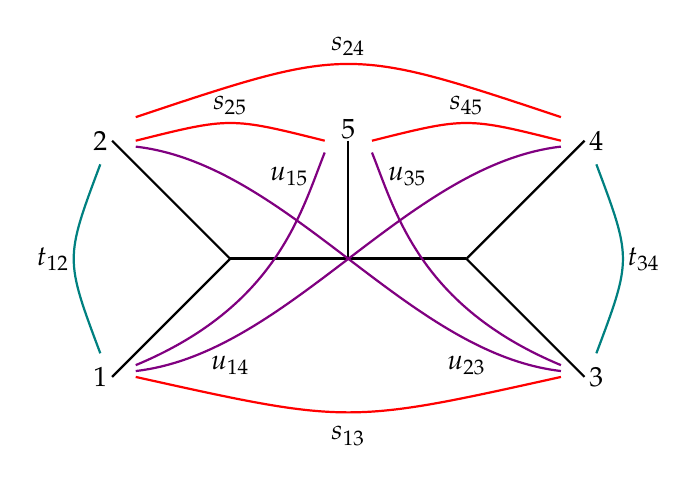
\begin{tikzpicture}[scale=1.5]

      \draw[thick] (-1,1)--(0,0);
      \draw[thick] (-1,-1)--(0,0);
      \draw[very thick] (0,0)--(1,0);
      \draw[thick] (1,1) -- (1,0);
      \draw[very thick] (1,0)--(2,0);
      \draw[thick] (2,0)--(3,1);
      \draw[thick] (2,0)--(3,-1);

      \node at (-1.1, 1) {2};
      \node at (-1.1, -1) {1};
      \node at (3.1, 1.0) {4};
      \node at (3.1, -1.0) {3};
      \node at (1, 1.1) {5};

      \draw[teal, thick] (-1.1,0.8)..controls (-1.4,0)..(-1.1,-0.8);
      \draw[teal, thick] (3.1,0.8)..controls (3.4,0)..(3.1,-0.8);
      \draw[red, thick] (-0.8,-1.0)..controls (1.,-1.4)..(2.8,-1);
      \draw[red, thick] (-0.8,1)..controls (0.,1.2)..(0.8,1.);
      \draw[red, thick] (1.2,1)..controls (2.,1.2)..(2.8,1.);
      \draw[red, thick] (-0.8,1.2)..controls (1.,1.8)..(2.8,1.2);
      \draw[violet,thick] (-0.8,-0.9)..controls (0.4,-0.4) and (0.6,0.4)..(0.8,0.9);
      \draw[violet,thick] (2.8,-0.9)..controls (1.6,-0.4) and (1.4,0.4)..(1.2,0.9);
      \draw[violet,thick] (2.8,-0.95)..controls (1.5,-0.8) and (0.5,0.8)..(-0.8,0.95);
      \draw[violet,thick] (2.8,0.95)..controls (1.5,0.8) and (0.5,-0.8)..(-0.8,-0.95);


      \node at (-1.5,0) {$t_{12}$};
      \node at (3.5,0) {$t_{34}$};
      \node at (1.,-1.5) {$s_{13}$};
      \node at (0, 1.3) {$s_{25}$};
      \node at (2,1.3) {$s_{45}$};
      \node at (1,1.8) {$s_{24}$};
      \node at (0,-0.9) {$u_{14}$};
      \node at (2,-0.9) {$u_{23}$};
      \node at (0.5,0.7) {$u_{15}$};
      \node at (1.5,0.7) {$u_{35}$};

    \end{tikzpicture}
  \end{subfigure}%
  \begin{subfigure}{0.5\textwidth}
    \centering
    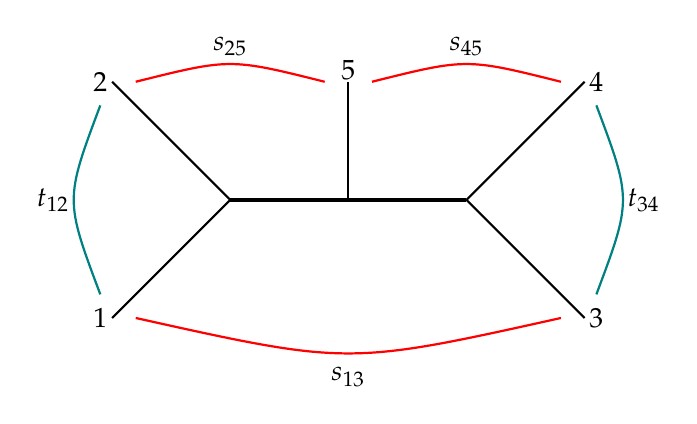
\begin{tikzpicture}[scale=1.5]

      \draw[thick] (-1,1)--(0,0);
      \draw[thick] (-1,-1)--(0,0);
      \draw[very thick] (0,0)--(1,0);
      \draw[thick] (1,1) -- (1,0);
      \draw[very thick] (1,0)--(2,0);
      \draw[thick] (2,0)--(3,1);
      \draw[thick] (2,0)--(3,-1);

      \node at (-1.1, 1) {2};
      \node at (-1.1, -1) {1};
      \node at (3.1, 1.0) {4};
      \node at (3.1, -1.0) {3};
      \node at (1, 1.1) {5};

      \draw[teal, thick] (-1.1,0.8)..controls (-1.4,0)..(-1.1,-0.8);
      \draw[teal, thick] (3.1,0.8)..controls (3.4,0)..(3.1,-0.8);
      \draw[red, thick] (-0.8,-1.0)..controls (1.,-1.4)..(2.8,-1);
      \draw[red, thick] (-0.8,1)..controls (0.,1.2)..(0.8,1.);
      \draw[red, thick] (1.2,1)..controls (2.,1.2)..(2.8,1.);

      \node at (-1.5,0) {$t_{12}$};
      \node at (3.5,0) {$t_{34}$};
      \node at (1.,-1.5) {$s_{13}$};
      \node at (0, 1.3) {$s_{25}$};
      \node at (2,1.3) {$s_{45}$};
    \end{tikzpicture}
  \end{subfigure}
  \caption{The ten two-body Mandelstam invariants of a five-point scattering amplitude (left) and our choice of five independent ones (right).}
  \label{fig:mandelstaminv5pt}
\end{figure}

As represented in figure \ref{fig:mandelstaminv5pt} (left), one can define  ten two-body Mandelstam invariants for a five-point function,
in an analogous way to the $2 \to 2$ scattering definition (\ref{eq:mandelstamst}), i.e.
\begin{equation}
  s_{ij}=-(k_i+k_j)^2\,,
\end{equation}
where $k_i$ are again external incoming momenta. Similarly, we define $t_{ij}$- and $u_{ij}$-type invariants.
Since not all the invariants are independent, we shall choose
the following five as independent, $s_{13},s_{25},s_{45},t_{12},t_{34}$, as shown in figure \ref{fig:mandelstaminv5pt} (right).
We will be focusing on the double Regge limit where $s_{25}, s_{45}\to \infty$, and necessarily $s_{13}\to \infty$, while $t_{12}$ and $t_{34}$ are held fixed.
It is also possible to define a single Regge limit by considering either $s_{25}\to \infty$ with $s_{13}/s_{25}$ also fixed, or $s_{45}\to \infty$ with $s_{13}/s_{45}$ fixed.\footnote{Another interesting limit to consider is the helicity-pole limit where $s_{25}\to \infty$ with $s_{13}/s_{25}\to \infty$ while $t_{12}, t_{34}$ and $s_{45}$ are fixed (or the one where  the roles of $s_{25}$ and $s_{45}$ are swapped). This limit is experimentally accessible in inclusive cross-sections~\cite{PhysRevLett.26.675}. It is also possible to consider the limit $s_{13}\to \infty$ with all the other Mandelstam invariants kept fixed.}
We note that the generalization of the double Regge limit to the case of $n$ identical massive particles is given by
\cite{Brower:1974yv},
% \begin{align}
% 	 & s \text{ type}
% 	 &                & t \text{ type}
% 	 &                & \omega \text{ type (Toller angles)} \nonumber     \\
% 	 & s_{r+1,r+3}^2
% 	 &                & s_{1,r+2}^2
% 	 &                & \frac{s_{p-2,p}^2 s_{p-1,p+1}^2}{s_{p-2,p+1}^2} .
% \end{align}
\begin{align}
 s \text{ type}:                       & \qquad s_{r+1,r+3} \,,                                     \\
 t \text{ type}:                       & \qquad      s_{1,r+2} \,,                                  \\
 \omega \text{ type (Toller angles)} : & \qquad   \frac{s_{p-2,p} s_{p-1,p+1}}{s_{p-2,p+1}} \,,
 \nonumber
\end{align}
where labels are in the following range $    r          =1,\cdots,n-3                                    ,\, p          =4,\cdots,n-1 $.
We also use $ s_{i,j}=-\left( k_{i+1}+\dots+k_j \right)^2 $.
% {\bf JVB: I removed the $n$-point generalizations of Mandelstam invariants as they don't correspond to ours in the 5-point case.}

Let us consider the partial-wave decomposition of an amplitude $ A =  A(s_{25}, s_{45},\eta; t_{12}, t_{34}) $ of five identical massive particles in
the  $t_{12}, t_{34}$ channels,
\begin{align}
  \label{eq:partialwavet12t34}
  A
  %  =\sum_{J_1=0}^{\infty}\sum_{J_2=0}^{\infty}\sum_{|m|<J_1, J_2}\left(\prod_{i=1}^{2} (2 J_i+1)\right) a_{J_1,J_2,m}(t_{12},t_{34}) e^{i m \theta_{\text{Toller}}}  d_{0 m}^{J_1}(\cos\theta_1)d_{m 0}^{J_2}(\cos\theta_2)\nonumber \\
  =\sum_{m=-\infty}^{\infty}\sum_{J_{1,2}=|m|}^{\infty} \prod_{i=1}^{2} (2 J_i+1) a_{J_1,J_2,m}(t_{12},t_{34}) z^{m} d_{0 m}^{J_1}(\cos\theta_1)d_{m 0}^{J_2}(\cos\theta_2)
  \,,
\end{align}
where  $\eta\equiv s_{13}/(s_{25}s_{45})$ and $z\equiv e^{i \theta_{\text{Toller}}}$, as defined below. Here $m$ denotes the allowed helicities of exchanged particles. 
% {\bf Should we use a different letter to avoid confusion with the mass $m$ later?}
We also use Wigner-$d$ functions which can be written in terms of Jacobi polynomials $\mathcal{P}_{J}^{\alpha,\beta}$ as
\begin{align}
  d_{m' m}^{J}(\cos\theta)=\left(\frac{\left(J+m\right)!\left(J-m\right)!}{\left(J+m'\right)!\left(J-m'\right)!}\right)^{\frac{1}{2}}\left(\sin \frac{\theta}{2}\right)^{m-m'}\left(\cos \frac{\theta}{2}\right)^{m+m'}\mathcal{P}_{J-m}^{m-m',m+m'}(\cos \theta)\,,
\end{align}
with
\begin{align}
  \mathcal{P}_{J}^{\alpha,\beta}(z)=\sum_ {n=0}^{J} \frac{(-1)^n}{n!} \frac{J!}{(J-n)!} \frac{\Gamma(n+\alpha+1)\Gamma(J-n+\beta+1)}{\Gamma(J+\alpha+\beta+2)} z^{n+\alpha} \left(1-z\right)^{J-n+\beta}
  .\end{align}
The scattering angles $\theta_1, \theta_2$ and $\theta_{\text{Toller}}$ have a clear physical meaning - see e.g.~\cite{Brower:1974yv}.
Consider the scattering process shown in the figure~\ref{fig:mandelstaminv5pt} with the exchanged momenta $q_1^2=t_{12}$ and $q_2^2=t_{34}$.
Firstly, we lump together particles $3,4$ and treat them as a single particle of momentum $q_2$.
The angle $\theta_1$ is defined as the scattering angle of the process $12\to 5 (34)$ which happens in a single plane in the center of mass frame.
Secondly, we consider the rest frame of the exchanged momentum $q_2$.
We denote the three momentum of particle-$i$ by $\vec{p}_i$.
As depicted in figure~\ref{fig:anglesframeq2}, we can choose a coordinate system where $\vec{p}_5$ is aligned with the $z$-axis and $\vec{p}_2$ lies somewhere in $xz$-plane.
We define $\theta_2$ as the zenith-angle of $ \vec{p}_3 $, whereas $\theta_{\text{Toller}}$ is the azimuth angle. Alternatively, the Toller angle can   be thought of as the angle
between the two scattering planes corresponding to the $q_1$ and $q_2$ rest frames, respectively.
\begin{figure}[t!]
  \centering
  \tdplotsetmaincoords{70}{170}
  \begin{tikzpicture}
    [scale=1.4,tdplot_main_coords, axis/.style={->,-latex',gray, opacity=0.6},
      vector guide/.style={dashed,red,thick},angle/.style={red,thick}]
    \draw[axis] (0,0,-1)--(0,0,3) node[anchor=west]{$z$};
    \draw[axis] (0,-2,0)--(0,5.5,0) node[anchor=west]{$y$};
    \draw[axis] (-4,0,0)--(4,0,0) node[anchor=south]{$x$};

    \draw[blue,ultra thick,->,-latex'] (0,0,0)--(0,0,1.5) node[anchor=west, blue] {$\vec{p}_{5}$};
    \tdplotsetcoord{P2}{2}{55}{180};
    \draw[blue,ultra thick,->,-latex'](0,0,0)--(P2) node[anchor=west, blue] {$\vec{p}_{2}$};
    \draw[vector guide] (0,0,0)--(P2xy);
    \draw[vector guide] (P2xy)--(P2);

    \tdplotsetcoord{P3}{6}{55}{60};
    \draw[blue,->,ultra thick,-latex'](0,0,0)--(P3) node[anchor=west,yshift=+2mm, blue] {$\vec{p}_{3}$};
    \draw[vector guide] (0,0,0)--(P3xy);
    \draw[vector guide] (P3xy)--(P3);

    \tdplotdrawarc[angle]{(0,0,0)}{1.5}{0}{60}{anchor=east,xshift=+2mm,yshift=-2mm}{$\theta_{\text{Toller}}$};
    \tdplotsetthetaplanecoords{55}
    \tdplotdrawarc[tdplot_rotated_coords,angle]{(0,0,0)}{1}{0}{55}{anchor=south east, xshift=+1mm,yshift=-1.5mm}{$\theta_{2}$};
  \end{tikzpicture}
  \caption{Scattering process shown in the resting frame of exchanged momentum $q_2$. This defines the angles $\theta_2$ and $\theta_{\text{Toller}}$. $ \theta_1 $ is defined analogously in the rest frame of exchanged momentum $q_1$.}
  \label{fig:anglesframeq2}
\end{figure}

The scattering angles are related to the Mandelstam invariants in a nontrivial way - see e.g. ~\cite{Weis:1972tbu,White:1973ola},
\begin{align}
  \label{eq:sijtoangles}
    & s_{25}= 2m^2+\frac{1}{2}\left(t_{34}-m^2-t_{12}\right)+\frac{1}{2}\left(\frac{(t_{12}-4m^2)\lambda(t_{12},t_{34},m^2)}{t_{12}}\right)^{1/2} \cos\theta_1\,,          \nonumber                  \\
    & s_{45}= 2m^2+\frac{1}{2}\left(t_{12}-m^2-t_{34}\right)+\frac{1}{2}\left(\frac{(t_{34}-4m^2)\lambda(t_{12},t_{34},m^2)}{t_{34}}\right)^{1/2} \cos\theta_2\,,           \nonumber                 \\
    & s_{13}=2m^2+\frac{1}{4}\left(m^2-t_{12}-t_{34}\right)+\frac{1}{4}\left(\frac{(t_{12}-4m^2)\lambda(t_{12},t_{34},m^2)}{t_{12}}\right)^{1/2} \cos\theta_1                                         \\
  + & \frac{1}{4}\left(\frac{(t_{34}-4m^2)\lambda(t_{12},t_{34},m^2)}{t_{34}}\right)^{1/2} \cos\theta_2+\frac{1}{4}\left(\frac{(t_{12}-4m^2)(t_{34}-4m^2)}{t_{12} t_{34}}\right)^{1/2}\times\nonumber \\
    & \left(m^2-t_{12}-t_{34}\right)\cos \theta_1 \cos \theta_2-\frac{1}{2}\left((t_{12}-4m^2)(t_{34}-4m^2)\right)^{1/2}\sin \theta_1\sin \theta_2 \cos\theta_{\text{Toller}}\,,\nonumber
\end{align}
where we use $\lambda(a,b,c)=a^2+b^2+c^2-2ab-2bc-2ca$. Note that here $m$ corresponds to the mass of the exchanged particles and should not be confused with helicity. We believe the context makes clear which one we refer to.
We emphasize that only $s_{13}$ depends on $\theta_{\text{Toller}}$.
Moreover, in the double Regge limit,
\begin{align}
  \label{eq:etaandToller}
  \eta\sim \frac{2(t_{12} t_{34})^{1/2}\cos \theta_{\text{Toller}}+m^2-t_{12}-t_{34}}{\lambda(t_{12},t_{34},m^2)}\,,
\end{align}
independently of $\theta_1$ and $\theta_2$.
This map suffers from some kinematical singularities in terms of the variables $t_{12}, t_{34}$.
These will be extracted from the possible types of singularities that we study below and we focus only on dynamical singularities.

To explore the double Regge region from the partial wave decomposition~(\ref{eq:partialwavet12t34}), we need a well-defined analytic continuation of the amplitude.
In contrast to the $2\to2$ scattering, for multiparticle scattering besides considering complex angular momentum, one also needs to account for helicity  dependence.
As stressed in~\cite{Goddard:1971fq, White:1972rq, White:1972sc, White:1973ola},  the analytic continuation of the amplitude to complex helicity values is also required.
The proper procedure for analytic continuation and its uniqueness deserve some comments.
Let us first review some concepts in the four-point case that will straightforwardly generalize to the five-point case we wish to analyse in more detail.
\begin{figure}[t!]
  \centering
  \begin{tikzpicture}
    \tikzset{middlearrow/.style={
          decoration={markings,
              mark= at position 0.8 with {\arrow{#1}} ,
            },
          postaction={decorate}
        }
    }
    \draw[] (-8,0)--(-4,0);
    \filldraw[black] (-4,0) circle (2 pt)node[anchor=south, yshift=2.5mm]{${ u=4m^2}$};
    \draw[] (2,0)--(6,0);
    \filldraw[black] (2,0) circle (2 pt) node[anchor=south, yshift=2.5mm]{${ s=4m^2}$};
    \draw[] (5.5,2.)--(6.,2.);
    \draw[] (5.5,2.5)--(5.5,2.);
    \node at (5.75,2.25) {$s$};

    \path [draw=red, middlearrow={<}]
    (-8.0,-0.5)..controls (-2.,-0.5) and (-2.,0.5) ..(-8.0,0.5);
    \path [draw=red, middlearrow={>}]
    (6.0,-0.5)..controls (0.,-0.5) and (0.,0.5) .. (6.0,0.5);



    \filldraw[black] (-2.,0) circle (2 pt) node[anchor=south,yshift=1.5mm]{$u_{0}$};
    \filldraw[black] (0,0) circle (2 pt)node[anchor=south,yshift=1.5mm]{$s_{0}$};

    \draw[red,<-] (-1.75,0) arc (0:360:0.25);
    \draw[red,<-] (0.25,0) arc (0:360:0.25);

  \end{tikzpicture}
  \caption{Singularities of $A(s,t)$ in the $s$ complex-plane at fixed $t$.}
  \label{fig:cutssplane}
\end{figure}

We assume that a $2\to2$ scattering amplitude has only singularities with dynamical origin. Namely, we only consider poles associated with bound states and branch-cuts starting at physical thresholds for particle production. In figure~\ref{fig:cutssplane} we depict these singularities at fixed $t$ in the complex $s$ plane. We assume that the following dispersion relation at fixed $t$ 
% {\bf I don't know who to cite here, this is standard once one assumes maximal analyticity...}
\begin{align}
  A(s,t) & =\frac{1}{2\pi i} \left(
  \int_{0}^{+\infty} \!\!\! ds' \, \frac{\text{Disc}_{s}(s',t,u')}{s'-s} + \int_{0}^{+\infty} \!\!\! du' \,\frac{\text{Disc}_{u}(s',t,u')}{u'-u} \right) =A_{R}(s,t)+A_{L}(u,t)\,.
\end{align}
Here, we have extended the notion of discontinuities $\text{Disc}_{s}$ and $\text{Disc}_{u}$ to include the contributions of bound-state poles.\footnote{We  assumed that no subtractions were needed in order to neglect contributions from arcs at infinity from the Cauchy integral that gives rise to the dispersion relation. If this is not the case, one should proceed considering instead a subtracted amplitude.}
We have also defined $A_{R}$ and $A_{L}$ with respect to each of the terms.
As it is clear from the definition, each of the terms has only cut contributions along one of the directions in the $s$ complex plane.
This fact is crucial in performing the analytic continuation of the amplitude with good large $J$ behaviour which happens to be unique as guaranteed by Carlson's theorem.
It is also useful to define the {\em signatured amplitude}~\footnote{The reader might be familiar with an equivalent decomposition of the full amplitude in terms of even and odd angular momentum contributions.
These are composed of signatured amplitudes.
Indeed we have $A^{\text{even}}=A^{+}(s,t)+A^{+}(-s,t)$ and $A^{\text{odd}}=A^{-}(s,t)-A^{-}(-s,t)$, where we use $u\sim-s$ in Regge limit.}
\begin{align}
  \label{eq:signaturedef}
  A^{\delta}(s,t)=\frac{1}{2}\big(A_{R}(s,t)+\delta\, A_{L}(s,t)\big) ,
\end{align}
where $\delta=\pm 1$.
Note that we replace $u$ by $s$ in $A_{L}$ ensuring that there are only cuts in a single direction.
The full amplitude can be easily reconstructed from the signatured amplitudes as
\begin{align}
  A(s,t)=\sum_{\delta=\pm 1}\left(A^{\delta}(s,t)+\delta\, A^{\delta}(u,t)\right) .
\end{align}
In what follows, we assume that the signatured amplitudes have the same analytic structure as the full amplitude.
%  While this assumption is consistent with the analytic structure of the full amplitude is not the only possibility.
This assumption greatly simplifies the discussion of dynamical singularities of partial-wave amplitudes.
We are entitled to consider the partial wave expansion of the signatured amplitude
\begin{align}
  \label{eq:partialwavesignature}
  A^{\delta}(s,t)=\sum_{J=0}^{\infty} (2J+1) a_{J}^{\delta}(t) P_{J}(z)\,.
\end{align}
Using the orthogonality of Legendre polynomials $P_J$ and (\ref{eq:signaturedef}), we can write
\begin{align}
  \label{eq:partialwavesignatureHelicity}
  a_{J}^{\delta}(t)=\frac{1}{4\pi i}\int_{z_0}^{+\infty} dz'\Big( \text{Disc}_{s}A_{R}(s',t)+\delta\,\text{Disc}_{s}A_{L}(s',t)\Big) Q_J(z')\,,
\end{align}
where $z_0$ is the branch point of the discontinuity and
$Q_J$ is the Legendre polynomial of the second kind  given by
\begin{align}
  Q_J(z) = \int_{-1}^{1} d\zeta \,\frac{P_J(\zeta)}{z-\zeta} \,.
\end{align}

\begin{figure}[t]
  \centering
  \begin{tikzpicture}
    \tikzset{middlearrow/.style={
          decoration={markings,
              mark= at position 0.77 with {\arrow{#1}} , mark=at position 0.25 with {\arrow{#1}},
            },
          postaction={decorate}
        }
    }
    \draw[->,gray, opacity=0.6,-latex'] (-1.0, 0.0)--(5.0,0.0);
    \draw[->,gray, opacity=0.8,-latex'] (0.0, -3.0)--(0.0,3.0);

    \filldraw[black] (0.0,0.0) circle (2pt);
    \filldraw[black] (1.0,0.0) circle (2pt);
    \filldraw[black] (2.0,0.0) circle (2pt);
    \filldraw[black] (3.0,0.0) circle (2pt);
    \filldraw[black] (4.0,0.0) circle (2pt);
    % \filldraw[black] (-1.0,0.0) circle (2pt);
    % \filldraw[black] (-2.0,0.0) circle (2pt);
    % \filldraw[black] (-3.0,0.0) circle (2pt);
    % \filldraw[black] (-4.0,0.0) circle (2pt);

    \draw[thick, black] (4.5,3.0)--(4.5,2.5)--(5.0,2.5) node[midway,anchor=south]{$J$};
    \path [draw=red,thick, middlearrow={latex'}] (-0.5, 3.0)--(-0.5,-3.0);
    \node[red] at (-0.8,2.7) {$C'$};
    \path [draw=blue, middlearrow={latex'}] (5.0, 0.5)..controls (-2.1,0.5) and (-2.1,-0.5)..(5.0,-0.5) node[blue,below,xshift=-1mm]{$C$};

    \filldraw[black] (1.0,1.5) circle (2pt);
    \draw[line width=0.7, red,<-,latex'-] (1.2, 1.5) arc (0:360:0.2);
  \end{tikzpicture}
  \caption{Contour integrals for the Sommerfeld-Watson transfom for the four partiacle scattering in the $J$-complex plane. As one deforms the contour from $C$ to $C'$ one has to consider the contribution from dynamical singularities which here we assume to be a Regge pole.
  }
  \label{fig:Jplane4pt}
\end{figure}
Using the symmetry $P_J(z)=(-1)^{J}P_J(-z)$, we perform a Sommerfeld-Watson transform of~(\ref{eq:partialwavesignature})
\begin{align}
  A^{\delta}(s,t)=\int_{C} \frac{dJ}{2\pi i} \frac{\pi}{\sin\pi J} \, (2J+1)a^{\delta}(J,t)P_{J}(-z) \,,
\end{align}
where $C$ is the closed contour depicted in figure~\ref{fig:Jplane4pt}. Due to the good large $J$ behaviour of the partial-wave $P_{J}$, one can continuously deform the contour from $C$ to $C'$, as
shown in the same figure.
We should account for all the possible singularities that   may be encountered during this deformation.
In this chapter, we always assume that these are pole type singularities \footnote{Other type of singularities like Regge cuts and nonsense-wrong-signature-fixed poles also exist. Moreover, singularities can also appear in a multiplicative manner but we neglect this scenario here for simplicity. The interested reader can find a discussion on those in~\cite{Weis:1972tbu} and references thereafter.}
\begin{align}
  a^{\delta}(J,t)\simeq \frac{\beta(t)}{J-\alpha(t)} \,,
\end{align}
where $\alpha(t)$ is a Regge trajectory and $\beta(t)$ is regular in $t$.
Regularity follows from the assumption that $A^{\delta}(s,t)$ has the same analytic structure of the full amplitude $A(s,t)$.
We also use the fact that Steinmann relations~\cite{SteinmannThesis} impose the latter to have no double discontinuity in $s$ and $t$.
At large $s$, we keep the rightmost pole as it gives the leading contribution and write
\begin{align}
  A^{\delta}(s,t)\sim \frac{1}{2\pi i}(-s)^{\alpha(t)} \Gamma\big(-\alpha(t)\big)\beta(t)\,,
\end{align}
where we   absorbed nonsingular factors into the definition of $\beta(t)$.

For the five-particle case  we expect a similar analytic structure of the amplitude in the $s_{25}, s_{45}$ and $s_{13}$ complex planes as in the four-particle case.
We would like to decompose the full amplitude in terms of signatured amplitudes with only right-hand or left-hand cuts for each $s$-type invariant.
We immediately see that we have to consider $2^3=8$ possible signatures.
Indeed, one writes
\begin{align}
  \label{eq:the8signatures}
   & A(s_{ij}, t_{ij})=  \sum_{\delta_{ij}=\pm 1} \left\{
  \left(A^{\delta_{25}\delta_{45}\delta_{13}}(s_{25},s_{45},\eta, t_{12},t_{34})+\delta_{25} A^{\delta_{25}\delta_{45}\delta_{13}} (-s_{25},s_{45},\eta, t_{12},t_{34}) + \right.\right. \\
   & \left.\left.  \delta_{45} A^{\delta_{25}\delta_{45}\delta_{13}} (s_{25},-s_{45},\eta, t_{12},t_{34}) +
  \delta_{25}\delta_{45} A^{\delta_{25}\delta_{45}\delta_{13}} (-s_{25},-s_{45},\eta, t_{12},t_{34})\right)+ \delta_{13} (\eta\to-\eta)
  \right\}\,,
  \nonumber
\end{align}
where we make a slight abuse of notation by writing $u_{ij}\sim-s_{ij}$ as dictated by the double-Regge limit we are exploring.
Indeed, note that each of the signatured amplitudes $A^{\delta_{25}\delta_{45}\delta_{13}}$ is a function with only right-hand cuts in each of the invariants $s_{25},s_{45}$ and $s_{13}$.
While $\delta_{25}, \delta_{45}$ are the already familiar signatures associated with angular momenta in the $t_{12}$ and $t_{34}$ channels,  $\delta_{13}$ is a new signature related to the helicity at the
central vertex.

\begin{figure}[t]
  \centering
  \begin{tikzpicture}
    %axis
    \draw[->,-latex',opacity=0.3] (0,0) -- (-3,0);
    \draw[->,-latex',opacity=0.3] (0,0) -- (0,3);
    \draw[->,-latex',opacity=0.3] (0,0) -- (0,-3);
    \draw[->,-latex',opacity=0.3] (0,0) -- (3,0);
    %points
    \draw[] (-1,3) -- (-1,2.5) -- (-1.5,2.5);
    \node[left] at (-1,2.8) {$ z $};
    \node[below right] at (2,0) {$ 1 $};
    \node[below right] at (4,-0.2) {$ a_> $};
    \node[below right] at (1,-0.2) {$ a_< $};
    % draw the point at origin and a circle around It 
    % \draw[thick,fill] (0,0) circle (0.1cm);
    %draw path
    % \draw[<-,line width=0.7,black ,latex'-] (0.4,0) to[out=90,in=0] (0,0.4) to[out=180,in=90] (-0.4,0) to[out=-90,in=180] (0,-0.4) to[out=0,in=-90] (0.4,0);
    \draw[line width=0.7,black ,-latex'] (2,0) to[out=90,in=0] (0,2) to[out=180,in=90] (-2,0) to[out=-90,in=180] (0,-2) to[out=0,in=-90] (2,0);
    \draw[thick,red,snake it] (0,0) -- (2,0);
    \draw[thick,blue,snake it] (2,0) -- (6,0);
  \end{tikzpicture}
  \caption{ Contour deformation in   $ z = e^{i \theta_{\mathtt{Toller}}} $ for doing the Froissart-Gribov continuation.
    The orthogonality relation holds on the black contours.
    We show the two different branch cuts corresponding to $ a_{\gtrless} $ discussed in (\ref{eq:aForsignaturedHelicity}).
  }
  \label{fig:tollerContour}
\end{figure}

Following~\cite{Goddard:1971fq}, we first analyse the analytic continuation of helicity $m$ to complex values.
Inspired by the form of the partial-wave decomposition~(\ref{eq:partialwavet12t34}), one expects the following dispersion relation to hold in the
$z$-complex plane, 
% this is not shown in this figure directly: as shown in figure \ref{fig:tollerContour},
\begin{equation}
  A(s_{ij},\eta, t_{ij})=\frac{1}{2\pi i} \left(\int_{-\infty}^{-1-\epsilon}+\int_{-1+\epsilon}^{1-\epsilon}+\int_{1+\epsilon}^{+\infty}\right)\frac{\text{Disc}_{z}A(s_{ij},\eta', t_{ij})}{z'-z}\,dz'\,.
\end{equation}
To have a well-defined analytic continuation, we need to consider amplitudes with cuts either only on the right or only on the left half plane in the respective Mandelstam variable.
Thus, we consider signatured amplitudes as introduced in~(\ref{eq:the8signatures}).
We can write
\begin{align}
  A^{\delta_{13}}(z)=\sum_{m=-\infty}^{+\infty} a_m^{\delta_{13}} z^{m}\,,
\end{align}
where we suppress the dependence on labels or parameters that are irrelevant for this discussion.
Using the fact that signatured amplitudes are functions with only right-hand cuts,~\footnote{Note that taking $z\to-z$ is related with $\eta\to -\eta$ as one can see from~(\ref{eq:etaandToller}).} we have
\begin{align}
  a_m^{\delta_{13}}=\left(\frac{1}{2\pi i}\right)^2 \left(\int_{0}^{1-\epsilon}+\int_{1+\epsilon}^{+\infty}\right)\int_{|z|=1}\frac{\text{Disc}_{z}A^{\delta_{13}}(z')}{z'-z} \, z^{-m-1}dz' dz\,.
\end{align}
For $z'>1$ and $m<0$ the $z$-integral gives 0, while for $m\ge0$, it gives $z'^{-m-1}$. On the other hand, if $0<z'<1$ and $m\ge 0$, the residues at the two poles cancel and the integral yields $ 0 $, whereas for $m<0$ we find $-z'^{-m-1}$.
We can then define, as shown in figure \ref{fig:tollerContour},
\begin{align}
  \label{eq:aForsignaturedHelicity}
   & a_{>}^{\delta_{13}}(m)=\frac{1}{2\pi i} \int_{1+\epsilon}^{\infty}(z')^{-m-1}\text{Disc}_{z}A^{\delta_{13}}(z') dz'\,, \\
   & a_{<}^{\delta_{13}}(m)=\frac{1}{2\pi i} \int_{0}^{1-\epsilon}(z')^{-m-1}\text{Disc}_{z}A^{\delta_{13}}(z')dz'\,,
\end{align}
where it is clear that $a_{>}^{\delta_{13}}$ has a good asymptotic behaviour in the right half-plane in the complex $m$ variable, whereas $a_{>}^{\delta_{13}}$ does so on the left-half plane.
We can thus perform a Sommerfeld-Watson transform in $m$ and write
\begin{align}
  A^{\delta_{13}}(z) & =\sum_{m=0}^{\infty}a_{>}^{\delta_{13}}(m) z^{m}-\sum_{m=-\infty}^{-1}a_{<}^{\delta_{13}}(m) z^{m}\nonumber                                                               \\
                     & =\frac{1}{2\pi i}\int_{C_R}dm\frac{\pi a_{>}^{\delta_{13}}(m)(-z)^m}{\sin \pi m}-\frac{1}{2\pi i}\int_{C_L}dm\frac{\pi a_{<}^{\delta_{13}}(m)(-z)^m}{\sin \pi m}\nonumber \\
                     & =\frac{1}{2\pi i}\int_{C}dm\frac{\pi \left(a_{>}^{\delta_{13}}(m)+a_{<}^{\delta_{13}}(m)\right)}{\sin \pi m}(-z)^m\,,
\end{align}
where the contours $C_R, C_L$ and $C$ are shown in figure~\ref{fig:ccontoursmplane}. Recovering the previously suppressed dependences and parameters, we have
\begin{figure}[t]
  \centering
  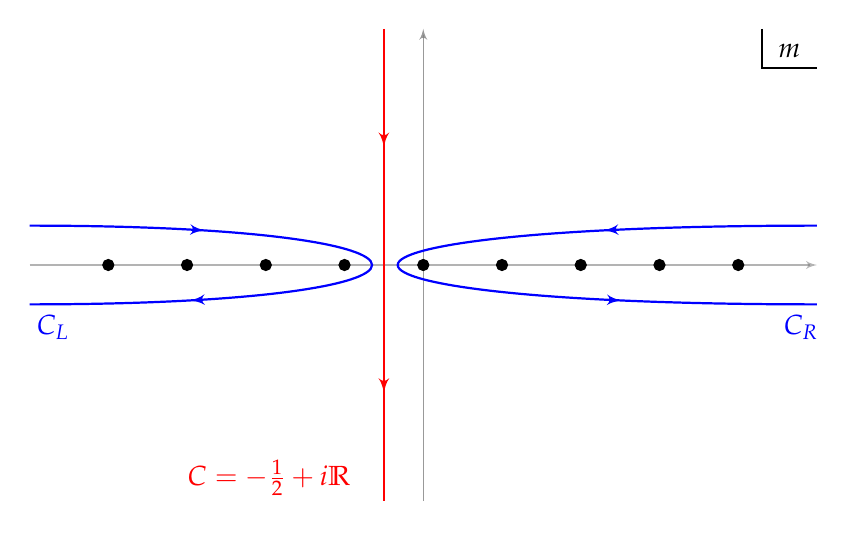
\begin{tikzpicture}
    \tikzset{middlearrow/.style={
          decoration={markings,
              mark= at position 0.77 with {\arrow{#1}} , mark=at position 0.25 with {\arrow{#1}},
            },
          postaction={decorate}
        }
    }
    \draw[-latex',gray, opacity=0.6] (-5.0, 0.0)--(5.0,0.0);
    \draw[-latex',gray, opacity=0.8] (0.0, -3.0)--(0.0,3.0);

    \filldraw[black] (0.0,0.0) circle (2pt);
    \filldraw[black] (1.0,0.0) circle (2pt);
    \filldraw[black] (2.0,0.0) circle (2pt);
    \filldraw[black] (3.0,0.0) circle (2pt);
    \filldraw[black] (4.0,0.0) circle (2pt);
    \filldraw[black] (-1.0,0.0) circle (2pt);
    \filldraw[black] (-2.0,0.0) circle (2pt);
    \filldraw[black] (-3.0,0.0) circle (2pt);
    \filldraw[black] (-4.0,0.0) circle (2pt);

    \draw[thick, black] (4.3,3.0)--(4.3,2.5)--(5.0,2.5) node[midway,anchor=south]{$m$};
    \path [draw=red,thick, middlearrow={latex'}] (-0.5, 3.0)--(-0.5,-3.0);
    % \node[purple] at (-0.8,2.7) {$C$};
    \node[red,left] at (-0.8,-2.7) {$C=-\frac{1}{2}+i \mathbb{R}$};
    \path [draw=blue,thick, middlearrow={latex'}] (5.0, 0.5)..controls (-2.1,0.5) and (-2.1,-0.5)..(5.0,-0.5) node[blue,below,xshift=-2mm]{$C_{R}$};
    \path [draw=blue,thick, middlearrow={latex'}] (-5.0, 0.5)..controls (0.8,0.5) and (0.8,-0.5)..(-5.0,-0.5) node[blue,below,xshift=+3mm]{$C_{L}$};
  \end{tikzpicture}
  \caption{Contour integrals for the Sommerfeld-Watson transfom in the $m$-complex plane.}
  \label{fig:ccontoursmplane}
\end{figure}
\begin{align}
  a_{\gtrless}^{\delta_{13}}(m) & = \sum_{J_1,J_2=m}^{\infty} \left(\prod_{i=1}^{2} (2 J_i+1)\right) a_{\gtrless,J_1,J_2,m}^{\delta_{25}\delta_{45}\delta_{13}}(t_{12},t_{34}) d_{0 m}^{J_1}(\cos\theta_1)d_{m 0}^{J_2}(\cos\theta_2)\,,
\end{align}
which only makes sense if we also analytically continue in the two angular momenta,
\begin{align}
   a_{\gtrless}^{\delta_{13}}(m)=\left(\prod_{i=1}^{2}\int_{C_i} \frac{dJ_i}{2\pi i} \frac{\pi(2 J_i+1)}{\sin \pi(J_i-m)}\right) a_{\gtrless}^{\delta_{25}\delta_{45}\delta_{13}}(J_1,J_2, m,t_{12},t_{34}) d_{0 m}^{J_1}(-z_1)d_{m 0}^{J_2}(-z_2)\,,
\end{align}
with contours $C_i$ as shown in figure~\ref{fig:jandmplanescontours} (left) and where $z_i=\cos\theta_i$.
%%%%%%%%%%%%%%%%%%%%%%%%%%%%%%%%%%%
%%%%%%%%%%%%%%%%%%%%%%%%%%%%%%%%%%%
\begin{figure}[t]
  \centering
  \begin{subfigure}{0.5\textwidth}
    \centering
    \begin{tikzpicture}
      \tikzset{middlearrow/.style={
            decoration={markings,
                mark= at position 0.5 with {\arrow{#1}} ,
              },
            postaction={decorate}
          }
      }
      \draw[->,gray, -latex',opacity=0.6] (-1.0, 0.0)--(5.0,0.0);
      \draw[->,gray, -latex',opacity=0.8] (0.0, -3.0)--(0.0,3.0);

      \filldraw[black] (1.0,0.0) circle (2pt) node[below,yshift=-0.8mm]{${\scriptstyle m}$};
      \filldraw[black] (2.0,0.0) circle (2pt)node[below]{${\scriptstyle m+1}$};
      \filldraw[black] (3.0,0.0) circle (2pt)node[below]{${\scriptstyle m+2}$};
      \filldraw[black] (4.0,0.0) circle (2pt)node[below]{${\scriptstyle m+3}$};

      \draw[thick, black] (4.5,3.0)--(4.5,2.5)--(5.0,2.5) node[midway,anchor=south,yshift=-1mm]{$J_i$};

      \path [draw=red,thick, middlearrow={latex'}] (0.5,3.0)--(0.5,1.7);
      \path [draw=red,thick, middlearrow={latex'}] (0.5,1.3)--(0.5,-3.0);
      \path[draw=red,thick] (0.5,1.7)..controls (1.4,1.7) and (1.4,1.3).. (0.5,1.3);
      \filldraw[black] (1.0,1.5) circle (2pt);

    \end{tikzpicture}
  \end{subfigure}%
  \begin{subfigure}{0.5\textwidth}
    \centering
    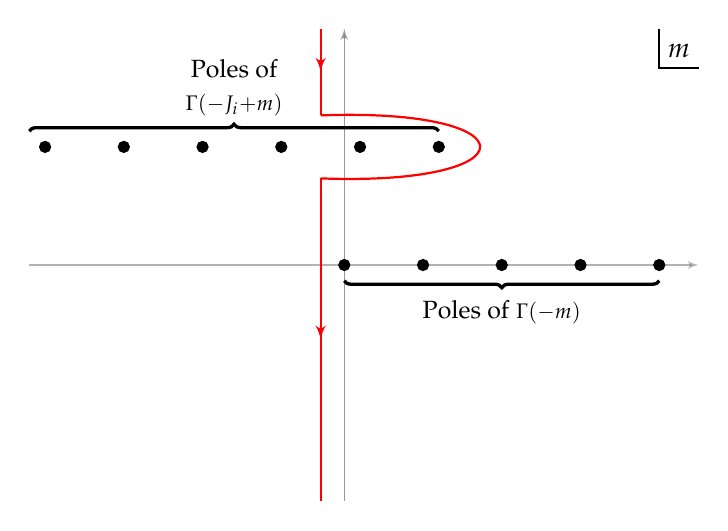
\begin{tikzpicture}
      \tikzset{middlearrow/.style={
            decoration={markings,
                mark= at position 0.5 with {\arrow{#1}} ,
              },
            postaction={decorate}
          }
      }
      \draw[->,gray,-latex', opacity=0.6] (-4.0, 0.0)--(4.5,0.0);
      \draw[->,gray, -latex',opacity=0.8] (0.0, -3.0)--(0.0,3.0);

      \filldraw[black] (0.0,0.0) circle (2pt);
      \filldraw[black] (1.0,0.0) circle (2pt);
      \filldraw[black] (2.0,0.0) circle (2pt);
      \filldraw[black] (3.0,0.0) circle (2pt);
      \filldraw[black] (4.0,0.0) circle (2pt);

      \draw[thick, black] (4.,3.0)--(4.,2.5)--(4.5,2.5) node[midway,anchor=south]{$m$};

      \path [draw=red,thick, middlearrow={latex'}] (-0.3,3.0)--(-0.3,1.9);
      \path [draw=red,thick, middlearrow={latex'}] (-0.3,1.1)--(-0.3,-3.0);
      \path[draw=red,thick] (-0.3,1.9)..controls (2.4,2) and (2.4,1).. (-0.3,1.1);

      \filldraw (1.2,1.5) circle(2pt);
      \filldraw (0.2,1.5) circle(2pt);
      \filldraw (-0.8,1.5) circle(2pt);
      \filldraw (-1.8,1.5) circle(2pt);
      \filldraw (-2.8,1.5) circle(2pt);
      \filldraw (-3.8,1.5) circle(2pt);
      \draw [decorate, very thick,
        decoration = {brace, mirror}] (0,-0.2) --  (4,-0.2);
      \node at (2.0,-0.6) {{\small Poles of} $ {\scriptstyle\Gamma(-m)}$};
      \draw [decorate, very thick,
        decoration = {brace,mirror}] (1.2,+1.7) --  (-4,1.7) node[midway,above]{\begin{tabular}{c} {\small Poles of}\\${\scriptstyle\Gamma(-J_i+m)}$\end{tabular}};
    \end{tikzpicture}
  \end{subfigure}
  \caption{Contour of integration in $J_i$ and $m$-complex planes when the respective variable is integrated first.
    Here, we only account for dynamical singularities given by Regge poles and ignore the existence of Regge cuts and fixed poles.
    Note that there are no dynamical singularities in the $m$-complex plane.}
  \label{fig:jandmplanescontours}
\end{figure}
%%%%%%%%%%%%%%%%%%%%%%%%%%%%%%%%%%%
%%%%%%%%%%%%%%%%%%%%%%%%%%%%%%%%%%%
% Note that while this seems very reasonable, the validity of such analytic continuation is very non-trivial.
This is a reasonable but non-trivial claim.
In fact, ~\cite{White:1972rq,White:1972sc} was only able to check a well-defined analytic continuation for a single angular momentum and helicity, but not the three simultaneously.
To the best of our knowledge, there is no derivation of the latter.
In the following, we assume that this defines a satisfactory analytic continuation of the signatured amplitude in terms of the scattering angles and of $t_{12}$ and $t_{34}$.
However, we would like to rewrite it in terms of the Mandelstam invariants alone.
This can be done by using the map   (\ref{eq:sijtoangles}).
To find the dependence on $s_{25}$ and $s_{45}$, we mimic the analysis of the four-particle case.
On the other hand, the $\eta$ dependence requires one more comment.
We assume that $A^{\delta_{13}}$ is an even function of the Toller angle and, in particular, a function of $\cos\theta_{\text{Toller}}$ (and thus invariant under $z\to 1/z$)\footnote{See~\cite{Weis:1972tbu} for whenever this is not the case.}.
This requirement follows from the realization that $\eta$ is an even function of $\theta_{\text{Toller}}$ and therefore only even functions of $\theta_{\text{Toller}}$ can be rewritten in terms of $\eta$.
This ends up imposing $a_{>}^{\delta_{13}}(m)=a_{<}^{\delta_{13}}(-m)$ and justifies dropping the subscripts when we write
\begin{align}
  A^{\delta_{13}}(\eta)=\frac{1}{2\pi i}\int_{C}dm\,\frac{\pi a^{\delta_{13}}(m)}{\sin \pi m}(-\eta)^m\,.
\end{align}
Note that, as we write $z$ in terms of $\eta$, we redefine what we mean by $a^{\delta_{13}}$.~\footnote{In particular, as commented before, there are kinematical singularities in the map that we shall ignore when we discuss dynamical singularities in $a^{\delta_{13}}(m)$.}
We can summarize the discussion on analytic continuations of five-particle amplitudes by writing
\begin{align}
  \label{eq:5ptreggeamplitude}
   & A^{\delta_{25}\delta_{45}\delta_{13}}(s_{25}, s_{45},\eta, t_{12}, t_{34})=\left(\frac{1}{2\pi i}\right)^{3}\int_C dm \left(  \prod_{i=1}^2   \int_{C_i} dJ_i  (2J_i+1)\right) \nonumber                 \\
   & \qquad\qquad \frac{\pi^3 d_{0 m}^{J_1}(-\cos\theta_1)d_{m 0}^{J_2}(-\cos\theta_2)(-\eta)^{m}}{\sin \pi m\sin \pi (J_1-m)\sin \pi(J_2-m)} \,a^{\delta_{25}\delta_{45}\delta_{13}}(J_1,J_2, m,t_{12},t_{34}) \nonumber \\
   & \qquad\qquad=\left(\frac{1}{2\pi i}\right)^{3}\int_C dm   \Gamma(-m)    \left(  \prod_{i=1}^2   \int_{C_i} dJ_i  (2J_i+1)\Gamma(-J_i+m) \right)                                                          \\
   & \qquad\qquad (-s_{25})^{J_1-m}(-s_{45})^{J_2-m}(-s_{13})^{m}a^{\delta_{25}\delta_{45}\delta_{13}}(J_1,J_2, m,t_{12},t_{34})\,,\nonumber
\end{align}
%\begin{align}
%	\label{eq:5ptreggeamplitude}
%	 & A^{\delta_{25}\delta_{45}\delta_{13}}(s_{25}, s_{45},\eta, t_{12}, t_{34})=\left(\frac{1}{2\pi i}\right)^{3}\int_C dm\int_{C_1} dJ_1\int_{C_2} dJ_2 (2J_1+1)(2J_2+1)\nonumber            \\
%	 & \frac{\pi^3 d_{0 m}^{J_1}(-\cos\theta_1)d_{m 0}^{J_2}(-\cos\theta_2)(-\eta)^{m}}{\sin m\sin (J_1-m)\sin(J_2-m)}a^{\delta_{25}\delta_{45}\delta_{13}}(J_1,J_2, m,t_{12},t_{34}),\nonumber \\
%	 & =\left(\frac{1}{2\pi i}\right)^{3}\int_C dm\int_{C_1} dJ_1\int_{C_2} dJ_2 (2J_1+1)(2J_2+1)\Gamma(-m) \Gamma(-J_1+m)\Gamma(-J_2+m)\nonumber                                               \\
%	 & (-s_{25})^{J_1-m}(-s_{45})^{J_2-m}(-s_{13})^{m}a^{\delta_{25}\delta_{45}\delta_{13}}(J_1,J_2, m,t_{12},t_{34})\,,
%\end{align}
where we used $\eta=s_{13}/(s_{25}s_{45})$ and
in the second equality $a^{\delta_{25}\delta_{45}\delta_{13}}(J_1,J_2, m,t_{12},t_{34})$ was redefined.

Under the assumption that the analytic continuation of the signatured amplitude has a good asymptotic behaviour in $J_1, J_2$ and $m$ such that we can ignore arcs at infinity, we focus on possible singularities that one might encounter as we move the contours to the left.
In figure~\ref{fig:jandmplanescontours}, we draw both $m$ and $J_i$ complex planes when the respective variable is integrated first.
In particular, we show the possible singularities.
As before, we restrict our analysis to Regge-pole-type of singularities and we refer interested readers to~\cite{Weis:1972tbu,Brower:1974yv} for more details on other type of singularities. 
%One expects that these singularities in $m$ are to the left of contour and that the asymptotic behaviour of the amplitude is completely determined by the dynamical singularities in angular momenta.
%There are two reasons for such an expectation. The
%first reason is tied to the consistency with the Steinmann relations.
%Note that the amplitude has the asymptotic behaviour {JVB: Changed it back to the previous text since the correction does not say what is intended below.}
One expects the singularities in $m$ to the left of contour and that determine the asymptotic behaviour of the amplitude to be completely determined by the dynamical singularities in angular momenta. The reason for that is bi-folded. First, note that the
amplitude has the asymptotic behaviour
\begin{align}
  (-s_{25})^{J_1-m}(-s_{45})^{J_2-m}(-s_{13})^{m}\,.
\end{align}
% For a limit where this is the dominant contribution, as it is the case of double-Regge limit, this expression might generically represent an amplitude which allows for a double discontinuity in two overlapping channel invariants,
Generically, this expression has a nonzero double discontinuity in the partially-overlapping channel invariants, namely $s_{25}$ and $s_{45}$.
However, this is forbidden by Steinmann relations~\cite{SteinmannThesis}.
Therefore, it must be that either $J_1-m$ or $J_2-m$ is a non-negative integer after the capture of poles.
It then follows that, in this limit, helicity singularities are fully determined by angular momentum ones as
\begin{align}
  m=\alpha-N\,,
\end{align}
where $\alpha$ is the location of a dynamical singularity in $J_1$ or $J_2$ and $N$ is a non-negative integer.
In the above argument, we naturally assume that the asymptotic behaviour is attained within a physical region for the amplitude.
It is conceivable, however, that such asymptotics do  not correspond to a physical behaviour and thus the argument would require an extension of validity of Steinmann relations for those configurations.
The second reason concerns the special nature of the helicity quantum number.
%    There are other arguments in favour of no dynamical singularities in helicity complex plane determining the asymptotic behaviour.
The physical interpretation of dynamical singularities are associated with the existence of particles.
As helicity is not a good Lorentz invariant and does not classify particles, as mass and spin do, we do not expect dynamical singularities in $m$~\cite{Brower:1974yv, Abarbanel:1972ayr}.
Besides, these assumptions seem to work well with specific models~\cite{Brower:1974yv,Schwarz:1973yz} as we will see below.

We now focus on our particular case of interest, the contribution of two Regge poles $\alpha_1(t)$ and $\alpha_2(t)$ in the double Regge limit with
\begin{align}
  a^{\delta_{25}\delta_{45}\delta_{13}}(J_1,J_2, m,t_{12},t_{34})\approx \frac{\beta(m, t_{12},t_{34})}{\big(J_1-\alpha_1(t_{12})\big)\big(J_2-\alpha_2(t_{34})\big)}\,.
\end{align}
In the Regge limit we move the $C_1$ and $C_2$ contours to the left in~(\ref{eq:5ptreggeamplitude}) and capture the poles in complex angular momentum. The leading contributions come from the rightmost poles. We find
\begin{align}
  \label{eq:5ptreggetheory}
   & A^{\delta_{25}\delta_{45}\delta_{13}}(s_{25}, s_{45},\eta, t_{12}, t_{34}) \sim\frac{1}{2\pi i}\int_C dm(2 \alpha_1+1)(2 \alpha_2+1)\Gamma(-m) \Gamma(-\alpha_1+m)\Gamma(-\alpha_2+m)\nonumber    \\
   & \qquad\qquad\qquad\qquad\qquad\qquad \times(-s_{25})^{\alpha_1-m}(-s_{45})^{\alpha_2-m}(-s_{13})^{m}\beta(m,t_{12},t_{34})\nonumber                                                   \\
   & \sim(-s_{25})^{\alpha_1}(-s_{45})^{\alpha_2} \left((-\eta)^{\alpha_1}\sum_{i}\Gamma(-\alpha_1+i)\Gamma(\alpha_1-\alpha_2-i)\beta(\alpha_1-i,t_{12},t_{34})\frac{\eta^{-i}}{i!}\right. \\
   & \qquad\qquad\qquad\qquad\quad
  \left.+(-\eta)^{\alpha_2}\sum_{i}\Gamma(-\alpha_2+i)\Gamma(\alpha_2-\alpha_1-i)\beta(\alpha_2-i,t_{12},t_{34})\frac{\eta^{-i}}{i!}\right).\nonumber
\end{align}
From the first to second line we closed the $C$ contour to the left, capturing all the $\alpha_i$-dependent poles, and absorbed overall constants into $\beta$.
In particular, if we consider the limit $\eta=s_{13}/(s_{25}s_{45})\to \infty$, we can just keep the leading contribution
\begin{align}
  A^{\delta_{25}\delta_{45}\delta_{13}}(s_{25}, s_{45},\eta, t_{12}, t_{34}) & \sim (-s_{13})^{\alpha_1}(-s_{45})^{\alpha_2-\alpha_1}\Gamma(-\alpha_1)\Gamma(\alpha_1-\alpha_2)\beta(\alpha_1,t_{12},t_{34})\nonumber \\
                                                                             & +(-s_{13})^{\alpha_2}(-s_{25})^{\alpha_1-\alpha_2}\Gamma(-\alpha_2)\Gamma(\alpha_2-\alpha_1)\beta(\alpha_2,t_{12},t_{34})\,,
\end{align}
which clearly does  not have double discontinuities in $s_{25}$ and $s_{45}$, as follows from our construction.
Note that the apparent singularities in $\alpha_1=\alpha_2$ are just spurious, as they cancel each other.

There are many subtleties and unproven statements in deriving the Regge theory result~(\ref{eq:5ptreggetheory}), but the final form seems very reasonable in physical terms.
We can analyze these claims in   specific models.
We consider a dual resonance model of a five-particle amplitude in the so-called Bardakci-Ruegg representation~\cite{Bardakci:1969ue}
%(see Appendix A of~\cite{Brower:1974yv} for more details on the following computations),
\begin{align}
  B_5 =  \int \frac{dx_1}{x_1}\, \frac{dx_2}{x_2}\, &
  x_1^{-\alpha(t_{12})} \left( 1-x_1 \right)^{-1-\alpha\left( s_{25} \right)}
  x_2^{-\alpha(t_{34})} \left( 1-x_2 \right)^{-1-\alpha\left( s_{45} \right)}
  \nonumber                                                                                                                                                                        \\
                                                    & \times \left( 1-x_1 x_2 \right)^{-\alpha\left( s_{13} \right) + \alpha\left( s_{25} \right) + \alpha\left( s_{45} \right) },
  \label{eq:BRrepresentation}
\end{align}
where the  integral ranges from $0$ to $1$ in $x_1$ and $x_2$. We defined   $\alpha(x)  = \alpha_0 + x$ with  $\alpha_0$  the intercept of the Regge trajectory.
As stated above, a single Regge limit happens when $ s_{25}$ (or  $s_{45}$),  $s_{13} \rightarrow \infty $ with their ratio fixed. In this limit, it can be shown  \cite{Brower:1974yv} that the region $ x_1 \approx 0 $ dominates in the integral~(\ref{eq:BRrepresentation}).
For the values $ 0<s_{25}/s_{13}<1 $, it can be shown that
\begin{align}
  B_5 =
  \left(
  -s_{13}
  \right)^{\alpha(t_{12})}
  \sum_{n=0}^{\infty} p_n \left( -\frac{s_{25}}{s_{13}} \right)^{n}
  +
  \left(
  -s_{13}
  \right)^{\alpha(t_{34})}
  \left(
  -s_{25}
  \right)^{\alpha(t_{12})-\alpha(t_{34})}
  \sum_{n=0}^{\infty} q_n \left( -\frac{s_{25}}{s_{13}} \right)^{n}
  ,\label{eq:singleReggeBR}
\end{align}
where
\begin{align}
  p_n (t_{12},t_{34}, s_{45}) & =
  \frac{\Gamma\big( n - \alpha(t_{12})\big)\, \Gamma( -n+t_{12}-t_{34})\, \Gamma\big( n - \alpha( s_{45} ) \big)}{\Gamma\big( t_{12}-t_{34}-\alpha( s_{45} ) \big) \, n!}\,,
  \\
  q_n (t_{12},t_{34}, s_{45}) & =
  \frac{\Gamma\big( n - \alpha(t_{34}) \big) \,\Gamma( -n+t_{34}-t_{12})\, \Gamma\big( n +t_{12}-t_{34}- \alpha( s_{45}) \big)}{\Gamma\big( t_{12}-t_{34}-\alpha( s_{45} ) \big) \, n!}\,.
  \label{eq:pqExpressions}
\end{align}
Note that there are no simultaneous singularities in the overlapping Mandelstam invariants.
This follows from the explicit expressions of $ p_n $ and $ q_n $.
The first term has power-law behaviour in $ s_{13} $ and poles in $s_{45} $, while having no singularities in $ s_{25} $.
The second term, on the other hand, has power-law behaviour in both $ s_{25} $ and $ s_{13} $ times a function without any singularities in $s_{45}$.
This is an instance of the Steinmann relations, which hold for the full amplitude.
The double Regge limit corresponds to taking a further limit $ s_{45} \rightarrow \infty $ with the ratio $\eta= s_{13}/\left( s_{25} s_{45} \right) $ fixed.
It leads to \cite{Brower:1974yv}
\begin{align}
  B_5 = \left( -s_{25} \right)^{\alpha(t_{12})} \left( -s_{45} \right)^{\alpha(t_{34})}
  \int_{-i \infty}^{i \infty}  \frac{dm}{2\pi i}  \, \Gamma\big( m- \alpha(t_{12}) \big)\Gamma\big( m- \alpha(t_{34}) \big)
  \Gamma (-m) \left( -\eta\right)^{m}\,,
  \label{eq:doubleReggeBR}
\end{align}
which is of the same form as~(\ref{eq:5ptreggetheory}).

With the knowledge of the multi-Regge limit in S matrix theory, we are now in a position to study the multi-Regge limit in conformal field theories.
%\section{Flat space scattering}\label{sec:FlatSpaceScattering}
%
%\begin{figure}[t]
%	\centering
%	\tdplotsetmaincoords{60}{125} % Set the viewpoint
%
%	\begin{tikzpicture}[tdplot_main_coords, scale=2]
%
%
%
%		\coordinate (O) at (0,0,0);
%		\coordinate (A) at (0,0,1);
%		\coordinate (B) at ( 1.48,1.49,1.71);
%		\coordinate (C) at ( 0,1.46 ,0.87);
%		\coordinate (D) at ( 1.48,1.49,0);
%		\coordinate (E) at ( 0,1.46 ,0);
%		% Draw the light blue xy plane
%		\fill[green!10,draw=none] (-2,-1,0) -- (2,-1,0) -- (2,2,0) -- (-2,2,0) -- cycle;
%		% Draw the x-axis
%		\draw[<->, latex'- latex'] (-2,0,0) -- (2,0,0) node[anchor=north east]{$x$};
%		% Draw the y-axis
%		\draw[->, - latex'] (0,0,0) -- (0,2,0) node[anchor=north west]{$y$};
%		% Draw the z-axis
%		\draw[->, - latex'] (0,0,0) -- (0,0,2) node[anchor=south]{$z$};
%		% Draw the three vectors that add up to zero
%		\draw[->,-latex', blue,  thick] (0,0,0) -- (0,0,1) node[anchor = south east] {$3$};
%		\draw[->,-latex', blue,  thick] (0,0,0) -- ( 1.48,1.49,1.71)node[anchor = south west] {$4$};
%		\draw[dashed  ] ( 1.48,1.49,0) -- ( 1.48,1.49,1.71);
%		\draw[dashed  ] ( 1.48,1.49,0) -- (0,0,0);
%		\draw[->,-latex', blue,  thick] (0,0,0) -- ( 0,1.46 ,0.87)node[anchor = north east] {$5$};
%		\draw[dashed] ( 0,1.46 ,0) -- ( 0,1.46 ,0.87);
%
%		\draw[->,-latex', red,  thick] (1,0,0)node[anchor = north west] {$1$} -- (0,0,0);
%		\draw[->,-latex', red,  thick] (-1,0,0)node[anchor = north] {$2$} -- (0,0,0);
%
%
%
%
%		\tkzMarkAngle[fill=orange,size=0.4cm, blue, thick ](B,O,A);
%		\tkzMarkAngle[fill=orange,size=0.2cm, thick ](D,O,E);
%
%	\end{tikzpicture}
%
%	\caption{We describe the frame of reference for the scattering of the five particles.
%		The kinematics is described by the two scattering angles and Toller angle.
%		We consider the process $ (1,2) \rightarrow (3,4,5) $ wherein the three point couplings are between $ (1,2,6), (3,4,7), (5,6,7) $.
%		In blue, we present the position part of the vectors $ p_3, p_4, p_5 $, the outgoing momenta in the rest frame of $ 7 $.
%		The black angle is the Toller angle.
%		In red, we present the rest frame of $ 6 $.
%		Note that these two frames are not identical and are related by a Lorentz transformation.
%	}
%	\label{fig:frameForFivePoints}
%\end{figure}
%
%In this section, we review the kinematics concerning the Regge theory in the Mandelstam variables \cite{Donnachie:2002en,Gribov:1961ex}.
%Regge limit probes the high energy regime of the scattering process.
%For the $ 2\rightarrow 2  $ scattering, it is parameterized in terms of $ s = \left(  k_1 + k_2 \right) ^{ 2} $ and $ t = \left(  k_1 + k_3 \right) ^{ 2} $, defined as a function of the momenta $ k_i $.
%In this case, $ s\rightarrow \infty $ while $ t $ fixed, plays the role of the Regge limit.
%
%% \todo[]{ {\color{red}\bf{V: references for multi-Regge; Do we need a discussion on the number of independent mandelstam invariants in terms of $d$?  A:Addressed  }}
%% }
%The generalization to higher point scattering amplitudes involves the following Mandelstam invariants \cite{Brower:1974yv,Bartels:2012gq,Caron-Huot:2020vlo}:
%\begin{align}
%	 & s \text{ type}
%	 &                & t \text{ type}
%	 &                & \omega \text{ type (Toller angles)} \nonumber     \\
%	 & W_{r+1,r+3}^2
%	 &                & W_{1,r+2}^2
%	 &                & \frac{W_{p-2,p}^2 W_{p-1,p+1}^2}{W_{p-2,p+1}^2} .
%\end{align}
%where $ W_{i,j}^2  = \left( k_{i+1}+\cdots + k_{j} \right)^2     $ is defined in terms of the external momenta, and labels are in the following range $    r          =1,\cdots,n-3                                    ,\, p          =4,\cdots,n-1 $.
%In words, $ s $ type invariants correspond to two body momenta just as in the case of four point scattering amplitude.
%However, $ t $ type invariants use $ r+1 $ momenta.
%For instance, $ W_{1,r+2}^{2}  = \left( k_{2} + \cdots + k_{r+2} \right)^{2}$.
%Unlike the case of two to two scattering, $ s $ and $ t $ are not on the same footing and therefore do not map to each other under crossing.
%
%% In $ d=4 $, this amounts to $ 3n-10 $ variables for $ n $-point scattering amplitude.
%% In $ d $-dimensional quantum field theories, the number of independent variables are $ n\left( n-1 \right)/3 $ when $ n<d+1 $, and otherwise $ \left( d-1 \right)n-d\left( d+1 \right)/2 $.
%For instance, for five point scattering amplitudes, the $ s $-type and $ t $-type invariants are as follows in terms of the external particles mass $ m $ :
%\begin{align}
%	s\text{-type} \,  &  & \left( k_3+k_4 \right)^2,\,  & \left( k_4+k_5 \right)^2       \\
%	t\text{-type}  \, &  & \left( k_2+k_3 \right)^2 ,\, & \left(k_2+ k_3+k_4 \right)^2 .
%\end{align}
%Apart from these, there is a specific ratio
%\begin{align}
%	\omega & =\frac{ \left(k_3+k_4\right)^2 \left(k_4+k_5\right)^2 }{\left( k_3+k_4+k_5 \right)^2}
%	.
%\end{align}
%that is kept fixed, even when both the numerators and the denominators approach $ \infty $.
%In this notation, the multi-Regge limit corresponds again to sending $ s$-type variable to $\infty $ while keeping other type of variables fixed.
%% Note that, while the $ s,t $  generalize the Mandelstam invariants for 4 point scattering, some properties related to crossing do not generalize.
%% In particular, $ 4! $ permutations of the external points permute $ s,t,u $  among themselves, in the 2 to 2 scattering.
%% However, the analogous $ 5! $  permutations do not permute $ s_r $  and $ t_r $  variables.
%% Therefore, we consider the Mandelstam invariants formed by product of two momenta $ k_i\cdot k_j$.
%
%
%In this section, we discuss the Regge limit and its generalization to multi-Regge limit in the specific case of string theory.
%We will consider the Regge limit of the string theory amplitude.
%First, we will consider the full amplitude using worldsheet methods.
%Then, we will use a particular limit of the Mandelstam invariants to arrive at the Regge limit of the amplitude from the partial wave analysis.
%% Second, we will use the coupling constants and masses on the leading Regge trajectory to directly find the Regge limit amplitude.  Third, we will use a particular generalization of OPE limit on the worldsheet to arrive at the same answer.
%
%% \todo[]{
%
%% 	{\color{red}\bf{V: The sentence below seems to be out of place; What are we scattering here? A:Addressed }}
%% }
%
%% The schematic formula for the $ n $-point scattering amplitude in string theory is \cite{Bjerrum-Bohr:2010pnr}
%% \begin{align}
%% 	T\left( k_{i,j}\right) & = \displaystyle\int \prod_{i=2}^{n-2} d^2 z_i \big|z_i\big| ^ {2 \alpha' k_1\cdot k_j} \big|z_i\big| ^ {2 \alpha' k_{n-1}\cdot k_i}\prod_{i<j\leq n-2} \big|z_j - z_i\big| ^ {2\alpha' k_i\cdot k_j}
%% 	.
%% \end{align}
%
%For concreteness, we review the case of four particle scattering amplitude in detail.
%In open string theory, the $ 2\rightarrow 2 $ scattering amplitude of particles with mass $ m $, with $ m^2 = -1/4 $ is schematically given by
%\begin{align}
%	T\left( s,t \right)=\sqrt{\pi}
%	% \frac{\left( \left( s t \right)^2 +\left( t u \right)^2 +\left( u s \right)^2 \right)}{stu}
%	\frac{
%		\Gamma\left(-\frac{s}{2} \right)
%		\Gamma\left(-\frac{t}{2} \right)
%		\Gamma\left(-\frac{u}{2} \right)
%	}{
%		\Gamma\left(\frac{1+s}{2} \right)
%		\Gamma\left(\frac{1+t}{2} \right)
%		\Gamma\left(\frac{1+u}{2} \right)
%	}
%	.
%	\label{eq:veneziano}
%\end{align}
%Here, the Mandelstam variables are constrained by $ s+t+u=-1$ in the units where $ \alpha' = 1 $.
%One can compute the Regge limit of this amplitude by sending $ s$ to infinity while keeping $t  $ fixed, by using the Stirling formula.
%
%Another way to understand this amplitude is to consider a particular channel and perform the partial wave expansion in terms of the harmonic polynomials of the scattering angle $ z= \cos\left( \theta \right) = 1+ 2s/\left( t+4 \right)$.
%\begin{align}
%	T\left( s,t \right) = \displaystyle\sum_{J=0}^{\infty}a_J\left( t \right)P_J\left( z \right)
%	.
%\end{align}
%The spectrum of the particle with mass $ M $ and spin $ J $ is encoded in the analytic structure of $ a_J\left( t \right) $, where the mass $ M  $ appears as a pole.
%From the formula, it is easy to see that $ M^2 = 2n $ with the corresponding residue $ \text{Res}_{t=2n} T = -2\left( 1+s \right)_{2n}/\left( 2n  \right)! $ with $ s =\left( n+2 \right)\left( z-1 \right)$.
%Note that the residue is a polynomial of degree $ 2n  $ in $ s $.
%These residues can be computed for a given $ z $ in terms of the partial wave expansion as follows,
%\begin{align}
%	\text{Res}_{t=2n} T\left( s,t \right) & =\displaystyle\sum_{J=0}^{\infty}P_J\left( z \right) \text{Res}_{t=2n} a_J\left( t \right)
%	=
%	-\frac{2\left( n+2 \right)^{2n}}{\left( 2n  \right)!}
%	z^{2n}
%	+ O\left( z ^ {2n-2} \right)
%	.
%	\nonumber
%\end{align}
%This implies that $ a_J\left( t \right) $ has poles at $ t=2n$ with $ n=J/2,J/2+1,\cdots $.
%The leading pole is given by
%\begin{align}
%	a_J\left( t \right) & \approx \frac{r\left( J \right)}{t-M ^ {2} \left( J \right)  }
%	, \,                &
%	\text{where }
%	M ^ {2}\left( J \right)  = J,                                                            r\left( J \right) = -\frac{2\left( 2J+2 \right)^{J}}{J!}
%	.
%\end{align}
%The information about only the leading pole is \textit{sufficient} to determine the Regge behavior of the full amplitude, since $ z \rightarrow \infty $ in the Regge limit.
%% \textbf{To be continued}
%
%% \Cref{eq:veneziano} is derived using the worldsheet analysis in string theory.
%% We would like to utilize it to directly arrive at the Regge limit $ s \rightarrow \infty $ with $ t $ fixed, \textit{without} calculating the full amplitude.
%% This exercise will be useful especially for the higher point case where the full amplitude is not known in terms of known mathematical functions.
%% Schematically, the integral representation for  (\ref{eq:veneziano}) is
%% \begin{align}
%% 	T\left( k_{i,j} \right) & = \int d^2 z |z|^{\alpha k_{3,1}} |1-z|^{\alpha k_{2,1}}
%% 	.
%% \end{align}
%% Here, $ k_{i,j} $ are defined as the product of the momenta $ k_i \cdot k_j $.
%% This involves saddle point analysis of the integral above.
%% If both the exponents are large, it is easy to show that the integral localizes at $ z=  k_{1,3}/(k_{1,3}+ k_{2,1}) $.
%% However, we are interested in a limit when $ k_{1,2} \rightarrow \infty $ with $ k_{1,3} $ fixed.
%% $ z \rightarrow 0 $ corresponds to such a limit.
%% Naively, this gets the contribution from one of the particles in the theory, which is the leading pole in $ k_{1,2} $ \cite{Brower:2006ea}.
%% However, we expect the whole leading Regge trajectory to contribute in the Regge limit.
%% It can be achieved by taking the limit $ z\rightarrow   0 $ with the product $ z \cdot k_{1,2} $ fixed.
%% This allows us to compute the Regge form, denoted by $T\left( s,t \right)^\mathcal{R}  $, of the amplitude directly to be \cite{Brower:2006ea,Costa:2012cb}
%% \begin{align}
%% 	T\left( s,t \right)^\mathcal{R} \approx \frac{\Gamma\left( {-\alpha' t/4} \right)}{\Gamma\left( {1+\alpha' t/4} \right)}\left( \frac{\alpha's}{4} \right) ^{2+\frac{\alpha' t}{4}}
%% 	.
%% \end{align}
%% The pole structure in the variable $ t $ is explicit in the $ \Gamma $ functions.
%
%% First, we consider the Veneziano formula for open string theory as a toy model of higher point analysis.
%% \begin{align}
%% 	A\left( s,t \right) & = \frac{\Gamma\left( -s \right) \Gamma\left( -t \right)}{\Gamma\left( -s-t \right)}
%% .
%% \end{align}
%
%% TODO: partial wave expansion.
%
%For the five point function, we discuss the generalization of this calculation\cite{Brower:1974yv}.
%Consider the following amplitude from open string theory called Bardakci-Ruegg representation
%\begin{align}
%	B_5 = \int
%	x_1^{-1-\alpha_1} \left( 1-x_1 \right)^{-1-\alpha\left( s_1 \right)}
%	x_2^{-1-\alpha_2} \left( 1-x_2 \right)^{-1-\alpha\left( s_2 \right)}
%	\left( 1-x_1 x_2 \right)^{-\alpha\left( s_{12} \right) + \alpha\left( s_1 \right) + \alpha\left( s_2 \right) }
%	.\label{eq:BRrepresentation}
%\end{align}
%Here, we use $ \alpha_i = \alpha_0 + t_i, \alpha\left( s \right)  = s+ \alpha_0 $, and the integral ranges from $0$ to $1$ in $x_1$ and $x_2$.
%This integral representation can be used to find the various limits of the amplitude $ B $, similar to the four point case.
%In the channel we are considering, the Mandelstam invariants suitable for Regge limit are as follows:
%\begin{align}
%	s_1 =k_2\cdot k_5 ,\,
%	s_2 =k_5\cdot k_4 ,\,
%	s_{12} =k_1\cdot k_3,\,
%	t_1=k_1\cdot k_2 ,\,
%	t_2 =k_3\cdot k_4
%	.\label{eq:mandInvs}
%\end{align}
%Simplest generalization of the Regge limit is single Regge limit, where $ s_1,s_{12} \rightarrow \infty $ with their ratio fixed.
%In this limit, it can be shown  \cite{Brower:1974yv} that the region $ x_1 \approx 0 $ dominates in the integral \cref{eq:BRrepresentation}.
%For the values $ 0<s_1/s_{12}<1 $, it can be shown that
%\begin{align}
%	B_5 =
%	\left(
%	-s_{12}
%	\right)^{\alpha_1}
%	\sum_{n=0}^{\infty} p_n \left( -\frac{s_1}{s_{12}} \right)^{n}
%	+
%	\left(
%	-s_{12}
%	\right)^{\alpha_2}
%	\left(
%	-s_{1}
%	\right)^{\alpha_1-\alpha_2}
%	\sum_{n=0}^{\infty} q_n \left( -\frac{s_1}{s_{12}} \right)^{n}
%	,\label{eq:singleReggeBR}
%\end{align}
%where,
%\begin{align}
%	p_n & =
%	\frac{\Gamma\left( n - \alpha_1 \right) \Gamma\left( -n+\alpha_1-\alpha_2 \right) \Gamma\left( n - \alpha\left( s_2 \right) \right)}{\Gamma\left( \alpha_1-\alpha_2-\alpha\left( s_2 \right) \right) \, n!},
%	\\
%	q_n & =
%	\frac{\Gamma\left( n - \alpha_2 \right) \Gamma\left( -n-\alpha_1+\alpha_2 \right) \Gamma\left( n -\alpha_2+\alpha_1- \alpha\left( s_2 \right) \right)}{\Gamma\left( \alpha_1-\alpha_2-\alpha\left( s_2 \right) \right) \, n!}
%	.\label{eq:pqExpressions}
%\end{align}
%
%Note that there are no simultaneous singularities in the overlapping Mandelstam invariants.
%This follows from the explicit expressions of $ p_n $ and $ q_n $.
%The first term has power law behavior in $ s_{12} $ and poles in $ s_2 $, while having no singularities in $ s_1 $.
%The second term has power law behavior in both $ s_1 $ and $ s_{12} $ times a function without any singularities in $ \alpha\left( s_2 \right) $.
%This is an instance of a much more general phenomenon, called `Steinmann relations', which hold for the full amplitude.
%We comment on it in \cref{app:steinmann}.
%
%Double Regge limit corresponds to taking a further limit $ s_2 \rightarrow \infty $ with the ratio $\omega= s_{12}/\left( s_1 s_2 \right) $ fixed.
%It leads to \cite{Brower:1974yv}
%\begin{align}
%	B_5 = \left( -s_1 \right)^{\alpha_1} \left( -s_2 \right)^{\alpha_2} \frac{1}{2\pi i}
%	\int_{-i \infty}^{i \infty}  d\lambda  \, \Gamma\left( \lambda- \alpha_1 \right)\Gamma\left( \lambda- \alpha_2 \right)
%	\Gamma\left( -\lambda \right) \left( -\omega\right)^{\lambda}
%	.\label{eq:doubleReggeBR}
%\end{align}
%
%This gives us the multi Regge form of the amplitude.
%Again, this integral can be computed by picking the poles in the first two Gamma functions, and closing the contour to the left.
%This also gives rise to a limiting amplitude that is consistent with Steinmann relations, as there are no triple power law singularities in $ s_1,s_2,s_{12} $.
%
%It would be interesting to reproduce this answer from Sommerfeld-Watson transform.
%One would need to find the partial wave coefficients in a closed form and analytically continue them in the respective quantum numbers.
%This is a non-trivial task, and we leave it for future work.
%
%
%Now, we provide a brief review of the S matrix Regge theory, without referring to any specific model such as string theory.
%The main goal is to describe the appropriate procedure to perform Sommerfeld-Watson transform.
%We review the various signatures involved in the Froissart-Gribov continuations of five point scattering amplitude in four dimensional quantum field theories, closely following \cite{Goddard:1971fq}.
%See also, \cite{White:1972sc,White:1973ola}.
%The reader familiar with the content may safely move to the next section.
%
%For the four particle case, we expand the amplitude, a function of Mandelstam invariants, in terms of the partial waves in one channel.
%\begin{align}
%	A\left( s,t \right) = \sum_{j=0}^{\infty} a_j\left( t \right) C_j\left( \cos \theta \right)
%	,\label{eq:4ptPartialWave}
%\end{align}
%where $ \cos \theta $ denotes the scattering angle in that channel.
%This admits Froissart-Gribov (FG) continuation in $ j $, for even and odd $ j $, separately.
%
%We discuss its generalization to five point amplitude, $ A\left( s_{12},s_1,s_2,t_1,t_2 \right) $.
%Here, $ s_{12},s_1,s_2 $ and $ t_1,t_2 $ (not written in the following equations for brevity) are the natural generalizations of $ s,t $, respectively, to five point functions \cite{Goddard:1971fq}.
%Let's denote the particle interacting with $ 1,2 $ be $ 6 $, as well as $ 3,4 $ be $ 7 $.
%Note that, the momentum conservation imposes constraints on the momenta of $ 6 $ and $ 7 $.
%We would like to define the scattering angles in the rest frame of $ 6 $ and $ 7 $.
%Let $ \zeta_1,\zeta_2 $ denotes these scattering angles.
%An important role is played by an invariant $ z = e^{i \theta_{\mathtt{Toller}}}  $, called Toller invariant.
%% ADD DISCUSSION OF THE FRAME AND INVARIANTS.
%Geometrically, $ \theta_{\mathtt{Toller}} $ denotes the angle between two scattering planes, one with $ 1,2 $ ingoing and another with $ 3,4 $ ingoing.
%
%Similar to \cref{eq:4ptPartialWave}, the five point amplitude can be expanded in partial waves.
%The coefficients of this expansion are labeled by the corresponding quantum numbers as $ a^{j_1,j_2}_{m} $
%The partial wave expansion is
%\begin{align}
%	A\left( \zeta_1,\zeta_2,z \right) = \sum_{j_1=0}^{\infty}  \sum_{j_2=0}^{\infty} \sum_{\left|m\right| <j_1,j_2} a_{m}^{j_1,j_2} z^m P_{j_1}^{-\left|m\right| }\left( \zeta_1 \right)P_{j_2}^{-\left|m\right| }\left( \zeta_2 \right)
%	.\label{eq:5ptPartialWaves}
%\end{align}
%Here, $ P_{j_1}^{-\left|m\right|} $ is a Legendre function.
%It is related to Jacobi polynomial as
%\begin{align}
%	P_j^{-n} \left( \zeta \right) \propto \left( \zeta^2-1 \right)^{ \frac{1}{2} n} P_{j-n}^{n,n}\left( \zeta \right)
%	.\label{eq:JacobiIdentity}
%\end{align}
%These polynomials admit a completeness property, which was used in writing \cref{eq:5ptPartialWaves}.
%This step also uses the orthogonality of power laws $ z^m $ and $ z^{-1-m} $ when integrated of unit circle $ \left|z\right| =1 $.
%We remind the reader that this is specific to four dimensioal quantum field theories.
%Precisely, in this dimensioal the relevant isometry group for Toller angle is $ SO(2)  $.
%In general dimensions $ d  $, the harmonic function on $ SO(d) $ are Gegenbauer polynomial.
%However, in $ d  = 2 $, they degenerate to Chebyshev polynomials which admit a simplification,
%\begin{align}
%	C_m \left( x  = \cos \left( \theta \right) \right)        & = \cos \left( m \theta \right)              \nonumber \\
%	C_m \left( \frac{1}{2} \left( z + z ^{-1} \right) \right) & = \frac{1}{2} \left( z^{m } + z^{-m} \right)
%	.
%\end{align}
%\begin{figure}[t]
%	\centering
%	\begin{tikzpicture}
%		%axis
%		\draw[->,-latex',opacity=0.3] (0,0) -- (-3,0);
%		\draw[->,-latex',opacity=0.3] (0,0) -- (0,3);
%		\draw[->,-latex',opacity=0.3] (0,0) -- (0,-3);
%		\draw[->,-latex',opacity=0.3] (0,0) -- (3,0);
%		%points
%		\draw[] (-1,3) -- (-1,2.5) -- (-1.5,2.5);
%		\node[left] at (-1,2.8) {$ z $};
%		\node[below right] at (2,0) {$ 1 $};
%		\node[below right] at (4,-0.2) {$ a_+ $};
%		\node[below right] at (1,-0.2) {$ a_- $};
%		% draw the point at origin and a circle around It 
%		% \draw[thick,fill] (0,0) circle (0.1cm);
%		%draw path
%		% \draw[<-,line width=0.7,black ,latex'-] (0.4,0) to[out=90,in=0] (0,0.4) to[out=180,in=90] (-0.4,0) to[out=-90,in=180] (0,-0.4) to[out=0,in=-90] (0.4,0);
%		\draw[line width=0.7,black ,-latex'] (2,0) to[out=90,in=0] (0,2) to[out=180,in=90] (-2,0) to[out=-90,in=180] (0,-2) to[out=0,in=-90] (2,0);
%		\draw[thick,red,snake it] (0,0) -- (2,0);
%		\draw[thick,blue,snake it] (2,0) -- (6,0);
%	\end{tikzpicture}
%	\caption{ Contour deformation in the $ z = e^{i \theta_{\mathtt{Toller}}} $ for doing the Froissart-Gribov continuation.
%		The orthogonality relation holds on the black contours.
%		We show the two different branch cuts corresponding to $ a_{\pm} $ discussed in \cref{eq:aPMcontour}.
%	}
%	\label{fig:tollerContour}
%\end{figure}
%Now, FG continuation takes place in two steps.
%First, we define
%\begin{align}
%	a_m\left( \zeta_1,\zeta_2 \right) =  \sum_{j_1=\left|m\right| }^{\infty}  \sum_{j_2=\left|m\right| }^{\infty} a_{m}^{j_1,j_2} P_{j_1}^{-\left|m\right| }\left( \zeta_1 \right)P_{j_2}^{-\left|m\right| }\left( \zeta_2 \right)
%	.\label{eq:5ptDefa}
%\end{align}
%This allows the partial wave expansion to be written as
%\begin{align}
%	A\left( \zeta_1,\zeta_2,z \right) = \sum_{m=-\infty}^{\infty} a_m \left( \zeta_1,\zeta_2 \right) z^{m}
%	.\label{eq:5ptExpansionNew}
%\end{align}
%\begin{figure}[t]
%	% \centering
%	\begin{subfigure}[]{0.5\textwidth}
%		\centering
%		\resizebox{\columnwidth}{!}{
%			\begin{tikzpicture}
%				%name
%				\draw[] (-1.2,3) -- (-1.2,2.5) -- (-2.5,2.5);
%				\node[left] at (-1.2,2.8) {$J_1,J_2$};
%				%axis
%				\draw[->,opacity=0.3,-latex'] (0,0) -- (-1.5,0);
%				\draw[->,opacity=0.3,-latex'] (0,0) -- (0,3);
%				\draw[->,opacity=0.3,-latex'] (0,0) -- (0,-3);
%				\draw[->,opacity=0.3,-latex'] (0,0) -- (5.8,0);
%				%drawing points 
%				% \draw[fill=black] (0,0) circle (0.05);
%				% \draw[fill=black] (1,0) circle (0.05);
%				\draw[fill=black] (2,0) circle (0.05);
%				\draw[fill=black] (3,0) circle (0.05);
%				\draw[fill=black] (4,0) circle (0.05);
%				\draw[fill=black] (5,0) circle (0.05);
%				\draw[fill=black] (0.3,1) circle (0.05);
%
%				% \draw[] (-0.662,0.830591) -- (-0.331,1.16178);
%				% \draw[] (-0.822,0.771524) -- (-0.272,1.32161);
%				% \draw[] (-0.9416,0.752275) -- (-0.252,1.44162);
%				% \draw[] (-1.0434,0.751257) -- (-0.251,1.5434);
%				% \draw[] (-1.133,0.761969) -- (-0.262,1.63345);
%				% \draw[] (-1.215,0.78141) -- (-0.281,1.71478);
%				% \draw[] (-1.289,0.807926) -- (-0.308,1.78902);
%				% \draw[] (-1.357,0.84052) -- (-0.341,1.85719);
%				% \draw[] (-1.420,0.878568) -- (-0.379,1.91991);
%				% \draw[] (-1.478,0.921687) -- (-0.422,1.97755);
%				% \draw[] (-1.530,0.96967) -- (-0.470,2.03033);
%				% \draw[] (-1.578,1.02245) -- (-0.522,2.07831);
%				% \draw[] (-1.621,1.08009) -- (-0.580,2.12143);
%				% \draw[] (-1.659,1.14281) -- (-0.643,2.15948);
%				% \draw[] (-1.692,1.21098) -- (-0.711,2.19207);
%				% \draw[] (-1.719,1.28522) -- (-0.785,2.21859);
%				% \draw[] (-1.738,1.36655) -- (-0.867,2.23803);
%				% \draw[] (-1.749,1.4566) -- (-0.9566,2.24874);
%				% \draw[] (-1.748,1.55838) -- (-1.0584,2.24772);
%				% \draw[] (-1.728,1.67839) -- (-1.178,2.22848);
%				% \draw[] (-1.669,1.83822) -- (-1.338,2.16941);
%				%drawing circles
%				% \draw[<-,line width=0.7,blue] (0.2,0) to[out=90,in=0] (0,0.2) to[out=180,in=90] (-0.2,0) to[out=-90,in=180] (0,-0.2) to[out=0,in=-90] (0.2,0);
%				% \draw[<-,line width=0.7,blue] (1.2,0) to[out=90,in=0] (1,0.2) to[out=180,in=90] (0.8,0) to[out=-90,in=180] (1,-0.2) to[out=0,in=-90] (1.2,0);
%				\draw[<-,line width=0.7,blue] (2.2,0) to[out=90,in=0] (2,0.2) to[out=180,in=90] (1.8,0) to[out=-90,in=180] (2,-0.2) to[out=0,in=-90] (2.2,0);
%				\draw[<-,line width=0.7,blue] (3.2,0) to[out=90,in=0] (3,0.2) to[out=180,in=90] (2.8,0) to[out=-90,in=180] (3,-0.2) to[out=0,in=-90] (3.2,0);
%				\draw[<-,line width=0.7,blue] (4.2,0) to[out=90,in=0] (4,0.2) to[out=180,in=90] (3.8,0) to[out=-90,in=180] (4,-0.2) to[out=0,in=-90] (4.2,0);
%				\draw[<-,line width=0.7,blue] (5.2,0) to[out=90,in=0] (5,0.2) to[out=180,in=90] (4.8,0) to[out=-90,in=180] (5,-0.2) to[out=0,in=-90] (5.2,0);
%
%				% \node[below] at (0.2,-0.1) {$\ell$};
%				% \node[below] at (1.2,-0.1) {$\ell+1$};
%				\node[below] at (2.2,-0.1) {$\mu$};
%				\node[below] at (3.2,-0.1) {$\mu+1$};
%				\node[below] at (4.2,-0.1) {$\mu+2$};
%				\node[below] at (5.2,-0.1) {$\mu+3$};
%				%main contour before deforming
%				\draw[->,line width=0.7,red] (0.5,1) to[out=90,in=0] (0.3,1.2) to[out=180,in=90] (0.1,1) to[out=-90,in=180] (0.3,0.8) to[out=0,in=-90] (0.5,1);
%				\draw[->,line width=0.7,red,-latex'] (-1,-3) -- (-1,3);
%
%				\node[above right] at (0.3,1.1) {$j(\nu)$};
%			\end{tikzpicture}
%		}
%		% \label{fig:contourDeformationJ1J2}
%	\end{subfigure}
%	\hfill
%	\begin{subfigure}[]{0.5\textwidth}
%		\centering
%		\resizebox{\columnwidth}{!}{
%			\begin{tikzpicture}
%				%name
%				\draw[] (-1,3) -- (-1,2.5) -- (-1.5,2.5);
%				\node[left] at (-1,2.8) {$\mu $};
%				%axis
%				\draw[->,opacity=0.3,-latex'] (0,0) -- (-1.5,0);
%				\draw[->,opacity=0.3,-latex'] (0,0) -- (0,3);
%				\draw[->,opacity=0.3,-latex'] (0,0) -- (0,-3);
%				\draw[->,opacity=0.3,-latex'] (0,0) -- (5.8,0);
%				%drawing points 
%				\draw[fill=black] (0,0) circle (0.05);
%				\draw[fill=black] (1,0) circle (0.05);
%				\draw[fill=black] (2,0) circle (0.05);
%				\draw[fill=black] (3,0) circle (0.05);
%				\draw[fill=black] (4,0) circle (0.05);
%				\draw[fill=black] (5,0) circle (0.05);
%				% \draw[fill=black] (0.3,1) circle (0.05);
%
%				% \draw[] (-0.662,0.830591) -- (-0.331,1.16178);
%				% \draw[] (-0.822,0.771524) -- (-0.272,1.32161);
%				% \draw[] (-0.9416,0.752275) -- (-0.252,1.44162);
%				% \draw[] (-1.0434,0.751257) -- (-0.251,1.5434);
%				% \draw[] (-1.133,0.761969) -- (-0.262,1.63345);
%				% \draw[] (-1.215,0.78141) -- (-0.281,1.71478);
%				% \draw[] (-1.289,0.807926) -- (-0.308,1.78902);
%				% \draw[] (-1.357,0.84052) -- (-0.341,1.85719);
%				% \draw[] (-1.420,0.878568) -- (-0.379,1.91991);
%				% \draw[] (-1.478,0.921687) -- (-0.422,1.97755);
%				% \draw[] (-1.530,0.96967) -- (-0.470,2.03033);
%				% \draw[] (-1.578,1.02245) -- (-0.522,2.07831);
%				% \draw[] (-1.621,1.08009) -- (-0.580,2.12143);
%				% \draw[] (-1.659,1.14281) -- (-0.643,2.15948);
%				% \draw[] (-1.692,1.21098) -- (-0.711,2.19207);
%				% \draw[] (-1.719,1.28522) -- (-0.785,2.21859);
%				% \draw[] (-1.738,1.36655) -- (-0.867,2.23803);
%				% \draw[] (-1.749,1.4566) -- (-0.9566,2.24874);
%				% \draw[] (-1.748,1.55838) -- (-1.0584,2.24772);
%				% \draw[] (-1.728,1.67839) -- (-1.178,2.22848);
%				% \draw[] (-1.669,1.83822) -- (-1.338,2.16941);
%				%drawing circles
%				\draw[<-,line width=0.7,blue] (0.2,0) to[out=90,in=0] (0,0.2) to[out=180,in=90] (-0.2,0) to[out=-90,in=180] (0,-0.2) to[out=0,in=-90] (0.2,0);
%				\draw[<-,line width=0.7,blue] (1.2,0) to[out=90,in=0] (1,0.2) to[out=180,in=90] (0.8,0) to[out=-90,in=180] (1,-0.2) to[out=0,in=-90] (1.2,0);
%				\draw[<-,line width=0.7,blue] (2.2,0) to[out=90,in=0] (2,0.2) to[out=180,in=90] (1.8,0) to[out=-90,in=180] (2,-0.2) to[out=0,in=-90] (2.2,0);
%				\draw[<-,line width=0.7,blue] (3.2,0) to[out=90,in=0] (3,0.2) to[out=180,in=90] (2.8,0) to[out=-90,in=180] (3,-0.2) to[out=0,in=-90] (3.2,0);
%				\draw[<-,line width=0.7,blue] (4.2,0) to[out=90,in=0] (4,0.2) to[out=180,in=90] (3.8,0) to[out=-90,in=180] (4,-0.2) to[out=0,in=-90] (4.2,0);
%				\draw[<-,line width=0.7,blue] (5.2,0) to[out=90,in=0] (5,0.2) to[out=180,in=90] (4.8,0) to[out=-90,in=180] (5,-0.2) to[out=0,in=-90] (5.2,0);
%
%				\node[below] at (0.2,-0.1) {$0$};
%				\node[below] at (1.2,-0.1) {$1$};
%				\node[below] at (2.2,-0.1) {$2$};
%				\node[below] at (3.2,-0.1) {$3$};
%				\node[below] at (4.2,-0.1) {$4$};
%				\node[below] at (5.2,-0.1) {$5$};
%
%
%				\node[left] at (-0.5,-3.0) {$\mathbf{V}= -\frac{1}{2} + i \mathbb{R}$};
%				%main contour before deforming
%				% \draw[->,line width=0.7,red] (0.5,1) to[out=90,in=0] (0.3,1.2) to[out=180,in=90] (0.1,1) to[out=-90,in=180] (0.3,0.8) to[out=0,in=-90] (0.5,1);
%				\draw[->,line width=0.7,red,-latex'] (-0.5,-3) -- (-0.5,3);
%
%				% \node[above right] at (0.3,1.1) {$j(\nu)$};
%			\end{tikzpicture}
%		}
%	\end{subfigure}
%	\caption{Contour deformation for the five point S-matrix. We only display the poles in $ \mu $ in the right half plane.
%	}
%	\label{fig:contourForSMatrix}
%\end{figure}
%FG continuation in $ m $ can be done as follows:
%\begin{align}
%	A\left( \zeta_1,\zeta_2,z \right) =-\frac{1}{2i} \int d\mu  \left( -z \right)^{\mu} \frac{a_+\left( \zeta_1,\zeta_2,\mu \right) + a_-\left( \zeta_1,\zeta_2,\mu \right)}{\sin \pi \mu}
%	.\label{eq:5ptExpansionNewWithFG}
%\end{align}
%The poles in $ \mu $ introduced by $ \sin \pi \mu $ lead to the poles in $ m $ in the formula \cref{eq:5ptExpansionNew}.
%The contour runs over $ \Re \mu = -\frac{1}{2} $.
%See \cite{White:1973ola}, for more details.
%Further, we use the analyticity \cite{White:1973ola} in this variable $ z $ to arrive at the FG representation above.
%\begin{align}
%	a_+\left( \zeta_i,\mu \right) & = \int_{1+\epsilon}^{\infty} dz\, z^{-1-\mu}  A\left( \zeta_i,z \right) \\
%	a_-\left( \zeta_i,\mu \right) & = \int_{0}^{1-\epsilon} dz\, z^{-1-\mu} A\left( \zeta_i,z \right)
%	.\label{eq:aPMcontour}
%\end{align}
%
%We can continue the functions $ a^{j_1,j_2}\left( \mu \right) $ in the variables $ j_1,j_2 $, respectively, using the techniques similar to the four point case.
%Since the analytic continuation happens again in the spin quantum numbers and the variable on which the polynomials depends are also the four point scattering angle analogues to the five point case, the same techniques can be used.
%% \todo[inline]{
%% 	Use White:1973ola
%% 	to write down more information about the analyticity in various variables
%% }
%
%Using the relation between the angle variables and the Mandelstam invariants, we arrive at the approximation of the amplitude in the multi Regge limit after picking possible dynamical poles in the variables $ J_1,J_2,\mu $.
%\begin{align}
%	A \approx s_1^{j_1^{*}} s_2^{j_2^{*}} \left( \frac{s_{12}}{s_1 s_2}  \right)^{m^{*}}
%	.\label{eq:regge5ptSmatrix}
%\end{align}
%However, the Steinmann relations, reviewed in \cref{app:steinmann}, impose a constraint on the allowed values of $ j_1^{*},j_2^{*},m^{*} $.
%In particular, simultaneous discontinuities in the variables $ s_1,s_{12} $ and $ s_2, s_{12} $ are not allowed.
%This means either $ j_1^{*}-m^{*} $ or $ j_2^{*}-m^{*} $ must be a positive integer.
%This implies that allowed locations of $ m^{*} $ are determined completely by the values of $ j_1^{*},j_2^{*} $.
%Note that, these relations are valid only in the physical region in a given channel.
%We have assumed that they continue to work in the asymptotic region under consideration.
%
%Inspired by these claims, we turn to the conformal field theory analogue of Regge theory.
%
%% \todo[]{
%% 	{\color{red}\bf{V: This part needs more details or a specific reference where the computation was done. \cite{Costa:2012cb} is cited for this computation but we did not do this directly from the integrand.  A: Addressed}}
%% }
%
%% Specifically, for the case of five points, using gauge fixing on the conformal group to fix points at $ z_1=0,z_4=1,z_5=\infty $, it reduces to
%% \begin{align}
%% 	T_5\left(k_{i,j} \right) =
%% 	\int d^2z_2 \, d^2z_3 \left| z_2-1\right| {}^{2 \alpha  k_{4,2}} \left| z_2\right| {}^{2 \alpha  k_{1,2}} \left| z_2-z_3\right| {}^{2 \alpha  k_{2,3}} \left| z_3-1\right| {}^{2 \alpha  k_{4,3}} \left| z_3\right| {}^{2 \alpha  k_{1,3}}
%% 	.
%% \end{align}
%% Note that we have used implicitly the momentum conservation to get rid of $ k_5 $ dependence.
%% We follow the standard technique of Schwinger parameters to evaluate these amplitudes.
%% This amounts to repeatedly using the following identity:
%% \begin{align}
%% 	z^{-a} = \frac{1  }{\Gamma\left( a \right)} \int_0^\infty d\alpha \,e^{-\beta z} \beta^{a-1}
%% 	.
%% 	\label{eq:Schwinger}
%% \end{align}
%
%
%
%% We use it for each distance between pairs of points, introducing Schwinger parameters $ \beta_{1,\dots,5} $.
%% Further, we use Gaussian integrals in order to evaluate all the spacetime integrals.
%% This leaves us with four integrals over $ \beta_{1,2,4,5} $ to determine the \textit{full} amplitude, schematically given by
%% % \todo[]{
%
%% % 	{\color{red}\bf{V: $ \mathcal{F}$ should be spelled out.  }}
%% % }
%
%% \begin{align}
%% 	T_5\left( k_{i,j} \right) & = \int_0^\infty d\beta_{1,2,4,5} \mathcal{F}_{\beta_{1,2,4,5}}\left( k_{i,j} \right)
%% 	\beta _1^{-k_{1,2}-1} \beta _2^{-k_{1,3}-1} \beta _4^{-k_{2,4}-1} \beta _5^{-k_{3,4}-1}
%% 	.
%% 	\label{eq:full5ptString}
%% \end{align}
%% Here, $ \mathcal{F}_{\beta_{1,2,4,5}} $ is defined as
%% \begin{align}
%% 	 &
%% 	\left(\beta _1 \left(\beta _2+1\right) \beta _5+\beta _1 \beta _4 \left(\beta _2+\beta _5+1\right)+\beta _2 \left(\beta _5 \beta _4+\beta
%% 	_4+\beta _5\right)\right){}^{k_{1,2}+k_{1,3}+k_{2,3}+k_{2,4}+k_{3,4}+2} \nonumber
%% 	\\
%% 	 &
%% 	\times
%% 	\left(\beta _4 \beta _2+\beta _2+\beta _4+\beta _4 \beta _5+\beta _5+\beta _1 \left(\beta _2+\beta
%% 	_5+1\right)\right){}^{-k_{1,2}-k_{1,3}-k_{2,3}-k_{2,4}-k_{3,4}-3}
%% 	\nonumber \\
%% 	 &
%% 	\times
%% 	\frac{\pi^2 \Gamma \left(-k_{1,2}-k_{1,3}-k_{2,3}-k_{2,4}-k_{3,4}-2\right)}{\Gamma \left(-k_{1,2}\right) \Gamma \left(-k_{1,3}\right) \Gamma
%% 		\left(-k_{2,3}\right) \Gamma \left(-k_{2,4}\right) \Gamma \left(-k_{3,4}\right)}
%% 	.
%% 	\label{eq:Ffunction}
%% \end{align}
%
%
%
%% The poles in $ k_{1,2},k_{3,4} $ correspond to the integrals over $ \beta_1,\beta_4 $ when the respective $ k $'s are negative integers.
%% Roughly, the poles exist for the same reason as they do for the Schwinger parameterization identity (\ref{eq:Schwinger}).
%% To evaluate the residues in these variables, we have to use integral by part several times and isolate the poles.
%% For instance, the residue in $ k_{1,2}$ and $k_{3,4} $ occur at integer values according to
%% \begin{align}
%% 	T_5 \equiv \sum_{n_1,n_2} \frac{ \mathcal{R}_{n_1,n_2}}{\left( k_{1,2} - n_1 \right) \left( k_{3,4} - n_2 \right) }
%% 	.
%% \end{align}
%% We refer to the \cref{ssec:residueComputation} for details of the residues $ \mathcal{R}_{n_1,n_2} $.
%
%% However, we are interested in the multi-Regge limit of this amplitude.
%% As prescribed earlier, it is a specific kinematic limit in which some of the $ k_{i,j} $'s blow up.
%% In particular, we have $ k_{1,2}$ and $k_{3,4} $ fixed while other invariants go to infinity.
%% To find the limiting value, we use the generalization of the worldsheet OPE analysis described above.
%% However, the naive OPE limit $z_2\to 0$ and $1-z_3 \to 0 $  of (\ref{eq:full5ptString}) does not give rise to the multi-Regge behavior.
%
%% The correct approach is similar to the four particle scattering case discussed above.
%% Since in this OPE limit $z_2\to 0$ and $1-z_3 \to 0 $, we have to account for the order of limit issue when the corresponding exponents go to $ \infty $.
%% We consider the multi-Regge kinematics defined earlier.
%% It can be shown that $ k_{1,3}$, $k_{2,3}$ and $k_{2,4} $ scale in the same manner to infinity.
%% Then we consider the integral as a function of $ k_{i,j} $ and discuss the multi-Regge limit.
%% First, we introduce Schwinger parameters $ x,y $ for $ |z_2| $ and $ |1-z_3| $, respectively.
%% Then, we observe that the remaining terms are of the form
%% \begin{align}
%% 	\left( 1+a \right)^b \approx e^{a b}
%% 	,
%% \end{align}
%% when we consider the region of integration of small $ a $ and large $ b $ with their product fixed.
%% This amounts to a saddle point evaluation of the integral when $z_2\to 0$ and $1-z_3 \to 0 $.
%% %It can be checked that it is indeed a saddle point by differentiating with respect to $ z,\bar{z},w,\bar{w}$, while treating them as independent variables.
%% Note that this is only one of the possible saddle points of the integrand.
%% % \todo[]{
%% % 	Check
%% % }
%% We find the following result:
%% \begin{align}
%% 	T_5\left( k_{i,j} \right) & =    \pi ^2 (-1)^{  2\alpha k_{2,4}} \frac{\Gamma\left( 1 + \alpha k_{1,2} \right)}{\Gamma\left( - \alpha k_{1,2} \right)} \frac{\Gamma\left( 1 + \alpha k_{3,4} \right)}{\Gamma\left( - \alpha k_{3,4} \right)}
%% 	\label{eq:5ptRegge}
%% 	\\
%% 	                          & \times 	 \left( -\alpha^{2} \left( k_{1,3} + k_{2,3} \right)^{2}\right) ^{-1-\alpha k_{3,4}}\left( -\alpha^{2} \left( k_{2,4} + k_{2,3} \right)^{2}\right) ^{-1-\alpha k_{1,2}}\,.
%% 	\nonumber
%% \end{align}
%
%
%
%% Some features of this amplitude are easy to notice.
%% For instance, the poles in $ k_{1,2}$ and $k_{3,4} $ are at negative integer values in the unit where $ \alpha'=1 $.
%
%
%
%% Alternatively, the residue admits the following partial wave representation.
%% \begin{align}
%% 	T_5 = \displaystyle\sum_{J_1,J_2=0}^{\infty}\displaystyle\sum_{\ell=0}^{\text{min} \left( J_1,J_2 \right)} a_{J_1,J_2,\ell} \left( t_1,t_2 \right)\mathcal{H}_{J_1,J_2,\ell}\left( Z_1,Z_2,Z_3 \right)
%% 	.
%% \end{align}
%
%
%% As shown in the \cref{app:HarmonicPoly}, the angle variables are defined as
%% \begin{align}
%% 	Z_1 & = \\
%% 	Z_2 & = \\
%% 	Z_3 & =
%% 	.
%% \end{align}
%% Again, the spectrum of the particles exchanged is encoded in $ a_{J_1,J_2,\ell} \left( t_1,t_2 \right)$.
%% For each triplet of spin quantum numbers, the leading behavior of the polynomial can be deduced from the explicit expression \ref*{eq:HPoly}.
%
%
%% {\color{red}\bf{V: I am not completely sure if this is the best way to present. As it is we first present Virasoro Shapiro for four pt. Then we do partial waves. Then we give the integral formula for four pts. Then we take Regge from integral representation. Then we  show the integral rep for $n$ points. We specify to $n=5$. Then we take Regge limit. And then partial waves.  }}
%
%
%
%% %%%%%%%%%%%%%%%%%%%%%%%%%%%%%%%%%%%%%%%
%
%% In this section, we review the kinematics concerning the Regge theory in the Mandelstam variables.
%% Regge limit probes the high energy regime of the scattering process.
%% For the $ 2\rightarrow 2  $ scattering, it is parameterized in terms of $ s = \left(  k_1 + k_2 \right) ^{ 2} $ and $ t = \left(  k_1 + k_3 \right) ^{ 2} $.
%% $ s\rightarrow \infty $ while $ t $ fixed, plays the role of the Regge limit.
%% The generalization to higher point scattering amplitudes involves the following Mandelstam invariants \cite{Brower:1974yv,Bartels:2012gq,Caron-Huot:2020vlo} :
%% \begin{align}
%% 	s_r       & =x_{r+1,r+3}^2                                   \\
%% 	t_r       & =x_{1,r+2}^2                                     \\
%% 	\omega_p  & =\frac{x_{p-2,p}^2 x_{p-1,p+1}^2}{x_{p-2,p+1}^2} \\
%% 	x_{i,j}^2 & = \left( k_{i+1}+\cdots + k_{j} \right)^2        \\
%% 	r         & =1,\cdots,n-3                                    \\
%% 	p         & =4,\cdots,n-1
%% 	.
%% \end{align}
%% In $ d=4 $, this amounts to $ 3n-10 $ variables for $ n $-point scattering amplitude.
%% In $ d $-dimensional quantum field theories, the number of independent variables are $ n\left( n-1 \right)/3 $ when $ n<d+1 $, and otherwise $ \left( d-1 \right)n-d\left( d+1 \right)/2 $.
%% In words, $ s $ type invariants correspond to two body momenta just as in the case of four point scattering amplitude.
%% However, $ t $ type invariants use $ r+1 $ momenta.
%% For instance, for five point scattering amplitudes, the kinematics are as follows in terms of the external particles mass $ m $ :
%% \begin{align}
%% 	s_1    & =2 k_3\cdot k_4-2 m^2                                                                                                            \\
%% 	s_2    & =2 k_4\cdot k_5-2 m^2                                                                                                            \\
%% 	t_1    & =2 k_2\cdot k_3-2 m^2                                                                                                            \\
%% 	t_2    & =-3 m^2+2 k_2\cdot k_3+2 k_2\cdot k_4+2 k_3\cdot k_4                                                                             \\
%% 	\omega & =\frac{\left(2 k_3\cdot k_4-2 m^2\right) \left(2 k_4\cdot k_5-2 m^2\right)}{-3 m^2+2 k_3\cdot k_4+2 k_3\cdot k_5+2 k_4\cdot k_5}
%% \end{align}
%% This can be inverted in terms of the mass of external particle $ m ^{2} $, as
%% \begin{align}
%% 	k_2\cdot k_3 & = m^2+\frac{t_1}{2},                                                           \\
%% 	k_2\cdot k_4 & = \frac{1}{2} \left(-m^2-s_1-t_1+t_2\right),                                   \\
%% 	k_3\cdot k_4 & = m^2+\frac{s_1}{2},                                                           \\
%% 	k_3\cdot k_5 & = \frac{s_1 \left(s_2-\omega \right)-\omega  \left(m^2+s_2\right)}{2 \omega }, \\
%% 	k_4\cdot k_5 & = m^2+\frac{s_2}{2}
%% 	.
%% \end{align}
%
%% In this notation, the multi-Regge limit corresponds again to $ s_r \rightarrow  \infty $ while keeping $ t_r ,\omega$ fixed.
%% Note that, while the $ s,t $  generalize the Mandelstam invariants for 4 point scattering, some properties related to crossing do not generalize.
%% In particular, $ 4! $ permutations of the external points permute $ s,t,u $  among themselves, in the 2 to 2 scattering.
%% However, the analogous $ 5! $  permutations do not permute $ s $  and $ t $  variables.
%
%% % For instance, one such permutation maps the above variables to
%% % \begin{align}
%% % 	s_1     \rightarrow & -3 m^2+s_{ 1 } \left(\frac{s_{ 2 }}{\omega }-1\right)-s_{ 2 },           \\
%% % 	s_2     \rightarrow & s_{ 2 },                                                                 \\
%% % 	t_1     \rightarrow & t_{ 1 },                                                                 \\
%% % 	t_2     \rightarrow & -3 m^2-s_{ 2 }+t_{ 1 }-t_{ 2 },                                          \\
%% % 	\omega  \rightarrow & \frac{-3 m^2 \omega -(s_{ 1 }+s_{ 2 }) \omega +s_{ 1 } s_{ 2 }}{s_{ 1 }}
%% % 	.
%% % \end{align}
%% Therefore, we consider the Mandelstam invariants formed by product of two momenta $ k_{i,j} $.
%
%% In this section, we discuss the Regge limit and its generalization to multi-Regge limit in the specific case of string theory.
%% We will consider the Regge limit of the string theory amplitude in three different ways.
%% First, we will consider the full amplitude using worldsheet method.
%% We will use a particular limit of the Mandelstam invariants to arrive at the Regge limit of the amplitude.
%% Second, we will use the coupling constants and masses on the leading Regge trajectory to directly find the Regge limit amplitude.
%% Third, we will use a particular generalization of OPE limit on the worldsheet to arrive at the same answer.
%
%% In type II superstring theory in $ 10 $ dimensions, the $ 2\rightarrow 2 $ scattering amplitude is given by
%% \begin{align}
%% 	T\left( s,t \right)=
%% 	8\pi G_N
%% 	\frac{\left( \left( s t \right)^2 +\left( t u \right)^2 +\left( u s \right)^2 \right)}{stu}
%% 	\frac{\Gamma\left( 1-\frac{\alpha' s}{4} \right)
%% 		\Gamma\left( 1-\frac{\alpha' t}{4} \right)
%% 		\Gamma\left( 1-\frac{\alpha' u}{4} \right)}{\Gamma\left( 1+\frac{\alpha' s}{4} \right)
%% 		\Gamma\left( 1+\frac{\alpha' t}{4} \right)
%% 		\Gamma\left( 1+\frac{\alpha' u}{4} \right)}
%% 	.
%% 	\label{eq:veneziano}
%% \end{align}
%% Here, the Mandelstam variables are constrained by $ s+t+u=4m^2 $, where $ m $ is the mass of the external particle.
%% Since, we consider dilatons, $ m=0 $.
%% We also use $ G_N $ to denote the Newton's constant.
%% One way to understand this amplitude and the spectrum of the particles exchanged is to consider a particular channel and perform the partial wave expansion in terms of the harmonic polynomials of the scattering angle $ z= \cos\left( \theta \right) = 1+2\frac{s}{t-4m^2}=1+\frac{2s}{t}$ as
%% \begin{align}
%% 	T\left( s,t \right) = \displaystyle\sum_{J=0}^{\infty}a_J\left( t \right)P_J\left( z \right)
%% 	.
%% \end{align}
%% The spectrum of the particle with mass $ M $ and spin $ J $ is encoded in the analytic structure of $ a_J\left( t \right) $, where the mass $ M  $ appears as a pole.
%% For the amplitude of dilatons, these poles lie at $ t=4n/\alpha' $. One can compute these residue for a given $ z $,
%% \begin{align}
%% 	\text{Res}_{t=4n/\alpha'} T & =\displaystyle\sum_{J=0}^{\infty}P_J\left( z \right) \text{Res}_{t=4n/\alpha'} a_J\left( t \right) \\
%% 	                            & =\frac{-128\pi G_N }{\left( \alpha' n \right)^2}\left( \frac{n z }{2}
%% 	\right)^{2n+2}+ O\left( z ^ {2n} \right)
%% 	.\end{align}
%% This implies that $ a_J\left( t \right) $ has poles at $ t=\frac{4 n}{\alpha'} $ with $ n=J/2-1,J/2,\cdots $.
%% The leading pole is given by
%% \begin{align}
%% 	a_J\left( t \right) & \approx \frac{r\left( J \right)}{t-M ^ {2} \left( J \right)  }
%% 	,\end{align}
%% where
%% \begin{align}
%% 	M ^ {2}\left( J \right) & = \frac{2\left( J-2 \right)}{\alpha'} & r\left( J \right) & =\frac{-128\pi G_N }{\left( \alpha' \Gamma\left( J/2 \right) \right)^2}\left( \frac{J-2 }{4}
%% 	\right)^{J}
%% 	.
%% \end{align}
%% The information about only the leading pole is \textit{sufficient} to determine the Regge behavior of the full amplitude.
%
%% \Cref{eq:veneziano} is derived using the worldsheet analysis in string theory.
%% We would like to utilize it to directly arrive at the Regge limit $ s \rightarrow \infty $ with $ t $ fixed, \textit{without} calculating the full amplitude.
%% This exercise will be useful especially for the higher point case where the full amplitude is not known in terms of known mathematical functions.
%% Schematically, the integral representation for \cref{eq:veneziano} is
%% \begin{align}
%% 	\int d^2 z |z|^{\alpha k_{3,1}} |1-z|^{\alpha k_{2,1}}
%% 	.
%% \end{align}
%% We can compute its Regge limit directly by doing the OPE analysis on the worldsheet.
%% This involves saddle point analysis of the integral above.
%% If both the exponents are large, it is easy to show that the integral localizes at $ z= \frac{k_{1,3}}{k_{1,3}+ k_{2,1}} $.
%% However, we are interested in a limit when $ k_{1,2} \rightarrow \infty $ with $ k_{1,3} $ fixed.
%% $ z \rightarrow 0 $ corresponds to such a limit.
%% Naively, this gets the contribution from one of the particles in the theory, which is the leading pole in $ k_{1,2} $ \cite{Brower:2006ea}.
%% However, we expect the whole leading Regge trajectory to contribute in the Regge limit.
%% It can be achieved by taking the limit $ z\rightarrow   0 $ with the product $ z \cdot k_{1,2} $ fixed.
%% This allows us to compute the Regge form, denoted by $T\left( s,t \right)^\mathcal{R}  $, of the amplitude directly to be \cite{Brower:2006ea,Costa:2012cb}
%% \begin{align}
%% 	T\left( s,t \right)^\mathcal{R} \approx \frac{\Gamma\left( {-\alpha' t/4} \right)}{\Gamma\left( {1+\alpha' t/4} \right)}\left( \frac{\alpha's}{4} \right) ^{2+\frac{\alpha ' s}{4}}
%% 	.
%% \end{align}
%% The pole structure in the variable $ t $ is explicit in the $ \Gamma $ functions.
%
%
%% We consider the higher point generalization of the analysis mentioned above.
%% The schematic formula for the string theory amplitude is \cite{Bjerrum-Bohr:2010pnr}
%% \begin{align}
%% 	T\left( k_{i,j}\right) & = \displaystyle\int \prod_{i=2}^{n-2} d^2 z_i \big|z_i\big| ^ {2 \alpha' k_1\cdot k_j} \big|z_i\big| ^ {2 \alpha' k_{n-1}\cdot k_i}\prod_{i<j\leq n-2} \big|z_j - z_i\big| ^ {2\alpha' k_i\cdot k_j}
%% 	.
%% \end{align}
%% Specifically, for the case of five points, using gauge fixing on the conformal group to fix points at $ z_1=0,z_4=1,z_5=\infty $, it reduces to
%% \begin{align}
%% 	T_5\left(k_{i,j} \right) =
%% 	\int d^2z_2 \, d^2z_3 \left| z_2-1\right| {}^{2 \alpha  k_{4,2}} \left| z_2\right| {}^{2 \alpha  k_{1,2}} \left| z_2-z_3\right| {}^{2 \alpha  k_{2,3}} \left| z_3-1\right| {}^{2 \alpha  k_{4,3}} \left| z_3\right| {}^{2 \alpha  k_{1,3}}
%% 	.
%% \end{align}
%% Note that we have used implicitly the momentum conservation to get rid of $ k_5 $ dependence.
%% We follow the standard technique of Schwinger parameters to evaluate these amplitudes.
%% This amounts to repeatedly using the following identity:
%% \begin{align}
%% 	z^{-a} = \frac{1  }{\Gamma\left( a \right)} \int_0^\infty d\alpha e^{-\beta z} \beta^{a-1}
%% 	.
%% \end{align}
%% We use it for each distance between pairs of points, introducing Schwinger parameters $ \beta_{1,\dots,5} $, as follows:
%% \begin{align}
%% 	\beta_1   &  & \beta_2   &  & \beta_3   &  & \beta_4   &  & \beta_5   \\
%% 	x^2_{1,2} &  & x^2_{1,3} &  & x^2_{3,2} &  & x^2_{2,4} &  & x^2_{3,4}
%% 	.
%% \end{align}
%% Here, $ x_{i,j} $ denote the distance between points $ i,j $.
%% Further, we use Gaussian integrals in order to evaluate all the spacetime integrals, leaving us with only the integrals over $ \beta $'s.
%% We then introduce a $ \delta $ function to introduce $ \lambda=\sum_{j=1}^{5} \beta_j $.
%% After changing the order of integration over $ \lambda $, we use the scaling in $ \beta $'s to set $ \beta_3=1 $.
%% This leaves us with four integrals over $ \beta_{1,2,4,5} $ to determine the \textit{full} amplitude.
%% \begin{align}
%% 	T_5\left( k_{i,j} \right) & = \int_0^\infty d\beta_{1,2,4,5} \mathcal{F}_{\beta_{1,2,4,5}}\left( k_{i,j} \right)
%% 	\beta _1^{-k_{1,2}-1} \beta _2^{-k_{1,3}-1} \beta _4^{-k_{2,4}-1} \beta _5^{-k_{3,4}-1}
%% 	.
%% 	\label{eq:full5ptString}
%% \end{align}
%
%% The poles in $ k_{1,2},k_{3,4} $ correspond to the integrals over $ \beta_1,\beta_4 $ when the respective $ k $'s are negative integers.
%% Roughly, the poles exist for the same reason as the Schwinger parameterization identity.
%% To evaluate the residues in these variables, we have to use integral by part several times and isolate the poles.
%% For instance, the residue in $ k_{1,2},k_{3,4} $ at $ n_1,n_2 $ is
%% \begin{align}
%% 	T_5 \equiv \sum_{n_1,n_2} \frac{ \mathcal{R}_{n_1,n_2}}{\left( k_{1,2} - n_1 \right) \left( k_{3,4} - n_2 \right) }
%% 	.
%% \end{align}
%
%% \todo[inline]{
%% 	Insert comments on the residues.
%% }
%
%% We are interested in the multi-Regge limit of this amplitude.
%% As prescribed earlier, it is a specific kinematic limit in which some of the $ k_{i,j} $'s blow up.
%% In particular, we have $ k_{1,2}, k_{3,4} $ fixed while others go to infinity.
%% To find the limiting value, we use the generalization of the worldsheet OPE analysis described above.
%% However, naive OPE limit $ z_2,1-z_3 \rightarrow 0 $  of equation \cref{eq:full5ptString} does not give rise to this behavior.
%
%% The correct approach is similar to the four particle scattering case discussed above.
%% Since in this OPE limit, $ z_2,1-z_3 \rightarrow 0 $ , we have to account for the order of limit issue when the corresponding exponents go to $ \infty $.
%% We consider the multi-Regge kinematics defined earlier.
%% It can be shown that $ k_{1,3},k_{2,3},k_{2,4} $ scale in the same manner to infinity.
%% The derivation follows the same logic as the four point case mentioned above.
%% We consider the integral as a function of $ k_{i,j} $ and discuss the multi-Regge limit.
%% First, we introduce Schwinger parameters $ x,y $ for $ |z_2| $ and $ |1-z_3| $, respectively.
%% Then, we observe that the remaining terms are of the form
%% \begin{align}
%% 	\left( 1+a \right)^b \approx e^{a b}
%% 	,
%% \end{align}
%% when we consider the region of integration of small $ a $ and large $ b $ with their product fixed.
%% This amounts to a saddle point evaluation of the integral when $ z_2,1-z_3 \rightarrow 0 $.
%% It can be checked that it is indeed a saddle point by differentiating with respect to $  z,\bar{z},w,\bar{w}$, while treating them as independent variables.
%
%
%% We find the following result:
%% \begin{align}
%% 	 & T_5\left( k_{i,j} \right)                                                                                                                                                                                                                                                                                                                                                               \\
%% 	 & =    \pi ^2 (-1)^{  2\alpha k_{2,4}} \frac{\Gamma\left( 1 + \alpha k_{1,2} \right)}{\Gamma\left( - \alpha k_{1,2} \right)} \frac{\Gamma\left( 1 + \alpha k_{3,4} \right)}{\Gamma\left( - \alpha k_{3,4} \right)} \left( -\alpha^{2} \left( k_{1,3} + k_{2,3} \right)^{2}\right) ^{-1-\alpha k_{3,4}}\left( -\alpha^{2} \left( k_{2,4} + k_{2,3} \right)^{2}\right) ^{-1-\alpha k_{1,2}}
%% 	.
%% 	\label{eq:5ptRegge}
%% \end{align}
%% Some features of this amplitude are easy to notice.
%% For instance, the poles in $ k_{1,2},k_{3,4} $ are at negative integer values in the unit where $ \alpha=1 $.
%
%
%
%% \todo[inline]{Outline the derivation of the expression above}
%% Alternatively, the residue admits the following partial wave representation.
%% \begin{align}
%% 	T_5 = \displaystyle\sum_{J_1,J_2=0}^{\infty}\displaystyle\sum_{\ell=0}^{\text{min} \left( J_1,J_2 \right)} a_{J_1,J_2,\ell} \left( t_1,t_2 \right)\mathcal{H}_{J_1,J_2,\ell}\left( Z_1,Z_2,Z_3 \right)
%% 	.
%% \end{align}
%
%% Here, the angle variables are defined as
%
%% \begin{align}
%% 	Z_1 & = -\frac{m^2 \omega -s_2 \omega +s_1 s_2+t_1 \omega }{2 \omega }, \\
%% 	Z_2 & = m^2+\frac{t_2}{2},                                              \\
%% 	Z_3 & = -\frac{m^2 \omega +(s_1+s_2) \omega -s_1 s_2}{2 \omega }
%% 	.
%% \end{align}
%% Again, the spectrum of the particles exchanged is encoded in $ a_{J_1,J_2,\ell} $.
%% The residue can be computed from the integral representation similar to the 4 particle scattering case.
%
%% \todo[inline,backgroundcolor=blue!20!white]{analogue of forward scattering theta going to 0.
%% 	Check if the H function simplifies in the Regge limit}
%% For each triplet of spin quantum numbers, the leading behavior of the polynomial can be deduced from the explicit expression \ref*{eq:HPoly}.
%% See the appendix on Harmonic polynomial.


%%%%%%%%%%%%%%%%%%%%%%%%%%%%%%%



%%%%%%%%%%%%%%%%%%%%%%%%%%%%%%%%



%%%%%%%%%%%%%%%%%%%%%%%%%%%%%%%%
\section{Kinematics of five-point conformal correlators}
\label{sec:KinematicsFivePointCorrelators}
%%%%%%%%%%%%%%%%%%%%%%%%%%%%%%%%

Correlation functions of local primary operators in any conformal field theory can be written in terms of a simple prefactor, that absorbs the weight of external operators, and a  non-trivial function that depends on conformal invariant variables, usually called cross ratios, that contains all the dynamics of the correlator.
In this chapter, we will be mostly focused in correlators involving five operators.
These depend on five different cross ratios through\footnote{This is the same number as independent Mandelstam invariants in flat space scattering amplitudes as reviewed in the previous section. The connection between correlation functions in conformal field theories and scattering amplitudes is more clear in Mellin space, as we shall see in the next section. }
\begin{align}
  \langle \mathcal{O}(x_1) \mathcal{O}(x_2) \mathcal{O}(x_3) \mathcal{O}(x_4) \mathcal{O}(x_5)  \rangle  = \frac{\left(\frac{x_{23}^2}{x_{13}^2}\right)^{\frac{\Delta_{12}}{2}} \left(\frac{x_{14}^2}{x_{13}^2}\right)^{\frac{\Delta_{34}}{2}}   }{(x_{12}^2)^{\frac{\Delta_1+\Delta_2}{2}}(x_{34}^2)^{\frac{\Delta_3+\Delta_4}{2}}} \left(\frac{x_{13}^2}{x_{15}^2x_{35}^2}\right)^{\frac{\Delta_5}{2}}\mathcal{G}(u_1\dots u_5)\,,
  \label{eq:fiveptcorrelatordef}
\end{align}
where $x_{ij}^2=(x_i-x_j)^2$, we used the shorthand notation $\Delta_{ij}\equiv \Delta_i-\Delta_j$ and the cross ratios are defined as
\begin{align}
  u_1= \frac{x_{12}^{2} x_{35}^{2}}{x_{13}^{2} x_{25}^{2}}\,,  \qquad\qquad u_{i+1} = u_{i}|_{x_{i} \rightarrow x_{i+1}}\,.
  \label{eq:crossRatiosuiFive}
\end{align}
It is worth emphasizing that this is just a particular choice of cross ratios which is obviously not unique.
For instance, $\tilde{u}_3\equiv u_3u_2$ would be as valid a choice as $u_3$.
The choice (\ref{eq:crossRatiosuiFive}) has the nice feature that the cross ratios can be defined by transforming the $x_i$ cyclically, {\em i.e.} $x_{i}\rightarrow x_{i+1}$.
This is particularly interesting when studying observables that are cyclically symmetric~\cite{Bercini:2020msp,Bercini:2021jti,Antunes:2021kmm}.

\begin{figure}[t!]
  % \centering
  % \begin{subfigure}[]{0.30\textwidth}
  % 	\centering
  % 	\resizebox{\columnwidth}{!}{
  % 		\begin{tikzpicture}
  % 			%draw a square with points at (2,0) (0,2) (0,-2) (-2,-2)
  % 			\draw[thick] (4,0) -- (0,4)  -- (-4,0) -- (0,-4)-- cycle;
  % 			\fill[green!10,draw=none]  (4,0) -- (0,4)  -- (-4,0) -- (0,-4)-- cycle;
  % 			%draw side bisectors
  % 			\draw[dashed,opacity=0.4] (2,2) -- (-2,-2);
  % 			\draw[dashed,opacity=0.4] (2,-2) -- (-2,2);
  % 			%points
  % 			\node[below] at (1.7,0) {$5$};
  % 			\draw[fill,black](1.7,0) circle (0.05cm);
  % 			\node[below] at (0.5,0) {$1$};
  % 			\draw[fill,black](0.5,0) circle (0.05cm);
  % 			\node[below] at (2.5,0) {$3$};
  % 			\draw[fill,black](2.5,0) circle (0.05cm);
  % 			% \node[below] at (2,-2.2) {$4^{-}$};
  % 			% \draw[fill,gray,opacity=0.4](2,-2.2) circle (0.05cm);
  % 			\node[below] at (-0.5,0) {$2$};
  % 			\draw[fill,black](-0.5,0) circle (0.05cm);
  % 			% \node[above] at (2,2.2) {$2^{+}$};
  % 			% \draw[fill,gray,opacity=0.4](2,2.2) circle (0.05cm);
  % 			\node[below] at (-2,0) {$4$};
  % 			\draw[fill,black](-2,0) circle (0.05cm);

  % 			%arrows for Regge 
  % 			\draw[->,opacity=0.4,-latex'] (0.5,0) to (0.1,0);
  % 			\draw[->,opacity=0.4,-latex'] (-0.5,0) to (-0.1,0);
  % 			% \draw[->,opacity=0.4,-latex'] (1.6,-1.1) to[out=270,in=135] (1.9,-1.7);
  % 			% \draw[->,opacity=0.4,-latex'] (-1.6,-1.1) to[out=270,in=45] (-1.9,-1.7);

  % 			\draw[opacity=0.4,thick,dashed] (4,-4) -- (4,4);
  % 			\draw[opacity=0.4,thick,dashed] (-4,-4) -- (-4,4);
  % 			%plot axis and label
  % 			% \draw[-stealth] (4.9,0) -- (4.9,0.5) node[anchor=south]{$ t $ };
  % 			% \draw[-stealth] (4.9,0) -- (5.4,0) node[anchor=south]{$ y $ };
  % 		\end{tikzpicture}
  % 	}
  % 	% \label{fig:contourDeformationJ1J2}
  % \end{subfigure}
  % \hfill
  % \begin{subfigure}[]{0.30\textwidth}
  % 	\centering
  % 	\resizebox{\columnwidth}{!}{
  % 		\begin{tikzpicture}
  % 			%draw a square with points at (2,0) (0,2) (0,-2) (-2,-2)
  % 			\draw[thick] (4,0) -- (0,4)  -- (-4,0) -- (0,-4)-- cycle;
  % 			\fill[green!10,draw=none]  (4,0) -- (0,4)  -- (-4,0) -- (0,-4)-- cycle;
  % 			%draw side bisectors
  % 			\draw[dashed,opacity=0.4] (2,2) -- (-2,-2);
  % 			\draw[dashed,opacity=0.4] (2,-2) -- (-2,2);
  % 			%points
  % 			\node[below] at (1.7,0) {$5$};
  % 			\draw[fill,black](1.7,0) circle (0.05cm);
  % 			\node[below] at (0.5,0) {$1$};
  % 			\draw[fill,black](0.5,0) circle (0.05cm);
  % 			\node[below] at (2.5,0) {$3$};
  % 			\draw[fill,black](2.5,0) circle (0.05cm);
  % 			% \node[below] at (2,-2.2) {$4^{-}$};
  % 			% \draw[fill,gray,opacity=0.4](2,-2.2) circle (0.05cm);
  % 			\node[above] at (-0.5,0) {$2$};
  % 			\draw[fill,black](-0.5,0) circle (0.05cm);
  % 			% \node[above] at (2,2.2) {$2^{+}$};
  % 			% \draw[fill,gray,opacity=0.4](2,2.2) circle (0.05cm);
  % 			\node[below] at (-2,0) {$4$};
  % 			\draw[fill,black](-2,0) circle (0.05cm);

  % 			%arrows for Regge 
  % 			\draw[->,opacity=0.4,-latex'] (0.5,0) to (0.5,0.5);
  % 			\draw[->,opacity=0.4,-latex'] (-0.5,0) to (-0.5,-0.5);
  % 			% \draw[->,opacity=0.4,-latex'] (1.6,-1.1) to[out=270,in=135] (1.9,-1.7);
  % 			% \draw[->,opacity=0.4,-latex'] (-1.6,-1.1) to[out=270,in=45] (-1.9,-1.7);

  % 			\draw[opacity=0.4,thick,dashed] (4,-4) -- (4,4);
  % 			\draw[opacity=0.4,thick,dashed] (-4,-4) -- (-4,4);
  % 			%plot axis and label
  % 			% \draw[-stealth] (4.9,0) -- (4.9,0.5) node[anchor=south]{$ t $ };
  % 			% \draw[-stealth] (4.9,0) -- (5.4,0) node[anchor=south]{$ y $ };
  % 		\end{tikzpicture}
  % 	}
  % \end{subfigure}
  % \vfill
  \centering
  \begin{subfigure}[]{0.5\textwidth}
    \centering
    \resizebox{\columnwidth}{!}{
      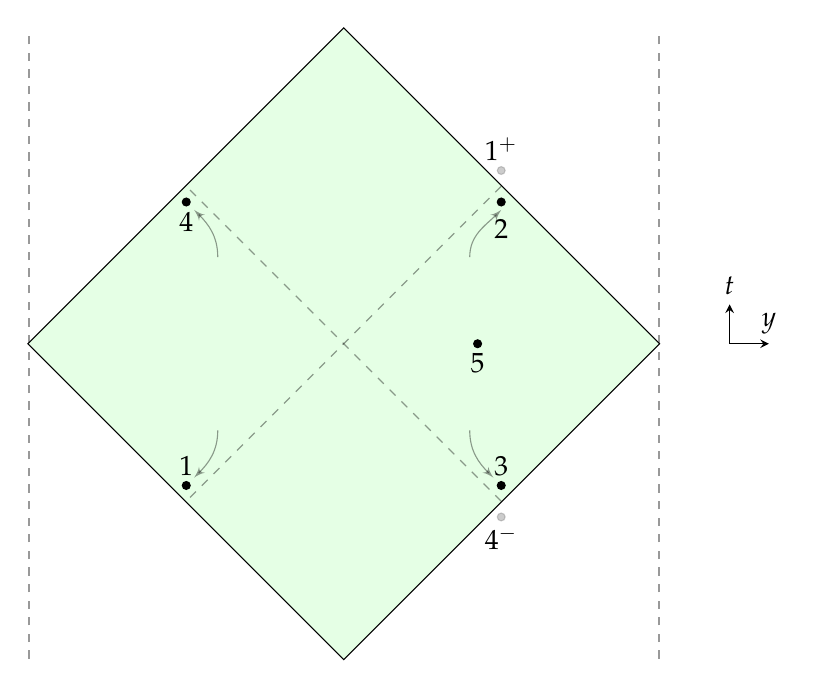
\begin{tikzpicture}
        %draw a square with points at (2,0) (0,2) (0,-2) (-2,-2)
        \draw[thick] (4,0) -- (0,4)  -- (-4,0) -- (0,-4)-- cycle;

        \fill[green!10,draw=none]  (4,0) -- (0,4)  -- (-4,0) -- (0,-4)-- cycle;
        %draw side bisectors
        \draw[dashed,opacity=0.4] (2,2) -- (-2,-2);
        \draw[dashed,opacity=0.4] (2,-2) -- (-2,2);
        %points
        % \node[below] at (0.7,0) {$5$};
        % \draw[fill,black](0.7,0) circle (0.05cm);

        \node[below] at (1.7,0) {$5$};
        \draw[fill,black](1.7,0) circle (0.05cm);

        \node[below] at (2,1.7) {$2$};
        \draw[fill,black](2,1.8) circle (0.05cm);
        \node[above] at (2,-1.8) {$3$};
        \draw[fill,black](2,-1.8) circle (0.05cm);
        \node[below] at (2,-2.2) {$4^{-}$};
        \draw[fill,gray,opacity=0.4](2,-2.2) circle (0.05cm);
        \node[above] at (-2,-1.8) {$1$};
        \draw[fill,black](-2,-1.8) circle (0.05cm);
        \node[above] at (2,2.2) {$1^{+}$};
        \draw[fill,gray,opacity=0.4](2,2.2) circle (0.05cm);
        \node[below] at (-2,1.8) {$4$};
        \draw[fill,black](-2,1.8) circle (0.05cm);

        %arrows for Regge 
        \draw[->,opacity=0.4,-latex'] (1.6,1.1) to[out=90,in=225] (2,1.7);
        \draw[->,opacity=0.4,-latex'] (-1.6,1.1) to[out=90,in=-45] (-1.9,1.7);
        \draw[->,opacity=0.4,-latex'] (1.6,-1.1) to[out=270,in=135] (1.9,-1.7);
        \draw[->,opacity=0.4,-latex'] (-1.6,-1.1) to[out=270,in=45] (-1.9,-1.7);

        \draw[opacity=0.4,thick,dashed] (4,-4) -- (4,4);
        \draw[opacity=0.4,thick,dashed] (-4,-4) -- (-4,4);
        %plot axis and label
        \draw[-stealth] (4.9,0) -- (4.9,0.5) node[anchor=south]{$ t $ };
        \draw[-stealth] (4.9,0) -- (5.4,0) node[anchor=south]{$ y $ };
      \end{tikzpicture}
    }
  \end{subfigure}
  \caption{
    We show our proposal for the Regge limit of the five-point correlator.
    % We compare our proposal with other interesting limits of the five point correlator:
    % 	Euclidean OPE limite (top left),   lightcone limit (top right) and  Regge limit (center).	
  }
  \label{fig:ReggeLimitVsOthers}
\end{figure}
In general, $\mathcal{G}(u_i)$ is an intricate function of the cross ratios with a complex analytic structure. One interesting question is, {\em what are the allowed singularities of a correlation function of five local operators and what is their physical meaning? }
This is a hard question that we will not try to answer here in full generality (see \cite{Maldacena:2015iua} for progress in this direction).
Instead, we shall focus on a particular singularity that is associated with the limit described in figure \ref{fig:ReggeLimitVsOthers} and that is similar to the Regge limit of scattering amplitudes reviewed in the previous section.
There are two other more common (and simpler) singularities, the Euclidean and lightcone OPE limits which will be relevant for the Regge limit analysis.
Indeed, it is possible to extract some information about these singularities from the conformal block decomposition of five points
\begin{align}
  \mathcal{G}(u_i)=  \sum_{k_1k_2,\ell}P_{k_1k_2 }^{\ell}G_{k_1k_2}^{\ell}(u_1,\dots u_5)\,,
  \label{eq:confblockDecom}
\end{align}
where $G_{k_1k_2}^{\ell}(u_1,\dots u_5)$ are conformal blocks in the channel $(12)$ and $(34)$, $P_{k_1k_2}^{\ell}$ are products of three-point coefficients (to be described in more detail in the following subsection) and the sum is over all primary operators.

In the following subsections, we will review and explore the Euclidean and lightcone singularities and introduce the Regge limit for five-point correlation functions.

%Other choices of cross ratios prove more useful in analyzing different physical settings as shall be seen below.  In the following subsections we will analyze distinct physical limits of the five point correlator (\ref{eq:fiveptcorrelatordef}) and explain the physics behind them. 



%%%%%%%%%%%%%%%%%%%%%%%%%%%%%%%%%%
\subsection{Euclidean limit}\label{subsec:Euclideanlimitsubsection}
%%%%%%%%%%%%%%%%%%%%%%%%%%%%%%%%%%
\begin{figure}[tbp]
  \centering
  % \includegraphics[width=0.3\textwidth]{figures/Cylinder}

  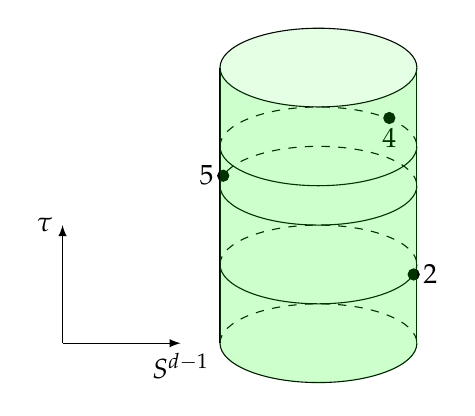
\begin{tikzpicture}
    \draw (0,0) ellipse (1.25 and 0.5);
    \draw (-1.25,0) -- (-1.25,-3.5);
    \draw (1.25,-3.5) -- (1.25,0);
    \filldraw[black ] (1.25 * 0.72, 0.5 *0.72-1 ) circle (2pt);

    \node[below] at(1.25 * 0.72, 0.5 *0.72 -1 ){$4$};
    \filldraw[black ] (1.25 * -0.967251, 0.5 *0.253823 -1.5 ) circle (2pt);
    \node[left] at (-1.25 * 0.967251, 0.5 *0.253823 -1.5 ){$5$};

    \filldraw[black ] (1.25 * 0.967251, -0.5 *0.253823 -2.5 ) circle (2pt);
    \node[right] at (1.25 * 0.967251, -0.5 *0.253823 -2.5 ){$2$};
    \draw[->,-latex] (-3.25,-3.5) -- (-3.25,-2);
    \draw[->,-latex] (-3.25,-3.5) -- ( -1.75 ,-3.5);

    \node[left] at (-3.25,-2) {$ \tau $};
    \node[below] at (-1.75, -3.5) {$ S^{d-1} $};

    \draw (-1.25,-1.5) arc (180:360:1.25 and 0.5);
    \draw [dashed] (-1.25,-1.5) arc (180:360:1.25 and -0.5);
    \draw (-1.25,-3.5) arc (180:360:1.25 and 0.5);
    \draw [dashed] (-1.25,-3.5) arc (180:360:1.25 and -0.5);

    \draw (-1.25,-1.0) arc (180:360:1.25 and 0.5);
    \draw [dashed] (-1.25,-1.0) arc (180:360:1.25 and -0.5);

    \draw (-1.25,-2.5) arc (180:360:1.25 and 0.5);
    \draw [dashed] (-1.25,-2.5) arc (180:360:1.25 and -0.5);
    \fill [green , opacity = 0.2] (-1.25,0) -- (-1.25,-3.5) arc (180:360:1.25 and 0.5) -- (1.25,0) arc (0:180:1.25 and -0.5);
    \fill [green , opacity = 0.1] (-1.25,0) arc (180:0:1.25 and 0.5) -- (-1.25,0) arc (180:0:1.25 and -0.5);

  \end{tikzpicture}
  \caption{Position of points on the Euclidean cylinder. Two points $ 1 $ and $ 3 $, are at $ \tau =  -\infty $ and $ \tau = \infty $.}
  % \caption{Cylinder picture of the five point correlation function}
  \label{fig:cylinder5point}
\end{figure}
The simplest limit in a CFT is when two operators are brought close to each other.
In this setup, the operator product expansion (OPE) is convergent and can be used safely.
%This is a  regime where the operator product expansion (OPE) can be used safely.
The OPE is perhaps one of the most important properties of a CFT.
This feature tells that the product of two operators at distinct points can be replaced by a linear combination of operators
\begin{align}
  \mathcal{O}(x_1)\mathcal{O}(x_2) \approx \sum_{k} \frac{C_{12k}}{(x_{12}^2)^{\frac{\Delta_1+\Delta_2-(\Delta_k-J_k)}{2}}}
  %	F_k \big(x_{12}\cdot D_{z},x_{12}\cdot\partial_{x_1},x_{12}^2 \partial_{x_1}\cdot D_{z},x_{12}^2\partial_{x_1}^2\big)\mathcal{O}_k(x_1,z)\,,
  F_k \big(x_{12}, D_{z},\partial_{x_1}\big)\mathcal{O}_k(x_1,z)\,,
  \label{eq:OPEequation}
\end{align}
where the sum runs over all primary operators, $C_{12k}$ are the OPE coefficients and $F_{k}$ is a differential operator that takes into account the contribution of descendants.
The auxiliary null variable $z$ is used to encode the open indices of a symmetric and traceless spin $J$ operator as
\begin{align}
  \mathcal{O}(x,z) \equiv z^{\mu_1}\dots z^{\mu_J} \mathcal{O}^{\mu_1\dots \mu_J}(x)\,,
\end{align}
while
\begin{align}
  D_{z^{\mu}} =\left( \frac{d}{2}-1+z\cdot\frac{\partial}{\partial z} \right)\frac{\partial}{\partial z^\mu}-\frac{1}{2} z^ \mu \frac{\partial^2}{\partial z \cdot \partial z}
  \label{eq:TodorovOPE}
\end{align}
is used to recover the information about the indices.
%The OPE  (\ref{eq:OPEequation}) is an operator equation that can be used inside a correlation function as long as it is possible to encircle the two operators at  $x_1$ and $x_2$ with a ball with some radius while leaving the other operators outside of it.
The exact form of $F_k$ can be determined from consistency of two- and three-point correlation functions of local operators.
It follows from a simple computation that, at the leading order and in the limit $x_2\rightarrow x_1$, the function $F_k$ is given by
\begin{align}
  F_k (x_{12}, D_{z},\partial_{x_1}) = \frac{(x_{12}\cdot D_{z})^{J_k}}{J_k!\left(\frac{d}{2}-1\right)_{J_k}} +\dots\,,
  \label{eq:OPEEuclideanLEading}
\end{align}
where $\dots$ represent  subleading terms.
One feature of this simple result is that it is evident that the limit is dominated by operators with lowest dimension $ \Delta_k $.
In particular, this determines the dominant contribution of a five-point conformal block  in the limits $x_{2}\rightarrow x_1$ and $x_4\rightarrow x_3$
\begin{align}
  \sum_{\ell} P_{k_1k_2}^{\ell}G_{k_1k_2}^{\ell}(u_1,\dots u_5) \approx \tfrac{C_{12k_1}C_{34k_2} (x_{12}\cdot D_{z})^{J_1}(x_{34}\cdot D_{z'})^{J_2}}{(x_{12}^2)^{\frac{J_{1}-\Delta_{k_1}}{2}} (x_{34}^2)^{\frac{J_{2}-\Delta_{k_2}}{2}}} \langle \mathcal{O}_{k_1}(x_1,z)\mathcal{O}_{k_2}(x_3,z') \mathcal{O}(x_5) \rangle\,.
  \label{eq:leadingtermOPEBoundaryCond}
\end{align}
Note that the double limit in the pair of points $(12)$ and $(34)$ was taken to reduce the correlator to a three-point function which is fixed by symmetry as
\begin{align}
   & \langle \mathcal{O}_{k_1}(x_1,z_1)\mathcal{O}_{k_2}(x_2,z_2) \mathcal{O}(x_3) \rangle  = \sum_{\ell=0}^{\textrm{min}(J_1,J_2)}\frac{C_{123}^{\ell} V_{123}^{J_1-\ell} V_{213}^{J_2-\ell} H_{12}^{\ell}}{(x_{12}^2)^{\frac{h_1+h_2-h_3}{2}} (x_{13}^2)^{\frac{h_1+h_3-h_2}{2}} (x_{23}^2)^{\frac{h_2+h_3-h_1}{2}}   } \,,
  \label{eq:threepontfunction}
\end{align}
where $h_i\equiv \Delta_i+J_i$ and
\begin{align}
   & H_{12} = (z_1\cdot x_{12})(z_2\cdot x_{12})- \frac{x_{12}^2  (z_1\cdot z_2)}{2}\,, \ \ \ \ \ V_{123} = \frac{(z_1\cdot x_{12} )x_{13}^2- (z_1\cdot x_{13})x_{12}^2}{x_{23}^2}\,.
\end{align}
It follows  from (\ref{eq:leadingtermOPEBoundaryCond}) that the constants $P_{k_1k_2}^{\ell}$ are given by
\begin{align}
  P_{k_1k_2}^{\ell} & =C_{12k_1}C_{34k_2}C_{k_1k_25}^{\ell} \,.
  \label{eq:OPE_coeffs}
\end{align}

Conformal blocks are complicated functions which are not known in closed form for general dimensions.
However, it is possible to compute them as an expansion around some limits.
One method to obtain them takes advantage of the fact that they are eigenfunctions of the conformal Casimir differential equation
\begin{align}
  \left(\mathcal{D}_{12} -c_{\Delta_{k_1},J_1}\right) G_{k_1k_2}^{\ell}=0\,,
\end{align}
with
\begin{align}
  c_{\Delta,J} =\Delta  (\Delta -d)+J (d+J-2)\,, \qquad
  \mathcal{D}_{12} = 2u_1^2\partial_{u_1}^2+\dots\,,
\end{align}
where $\dots$ represent other subleading terms.
%  which are spelled out in appendix \ref{app:CasimirEquationDetails}. \textbf{AS:appendix to be added.Is it necessary?}
We omitted an analogous equation in the $(34)$ channel that can be obtained using symmetry.

The cross ratios (\ref{eq:crossRatiosuiFive}) are not appropriate for all situations.
For instance, in the limit considered above where $x_2\rightarrow x_1$ and $x_4\rightarrow x_3$, one has
\begin{align}
  u_1,u_3\rightarrow 0\,, \ \ \ \  \ \ \ u_i\rightarrow 1 \ \ \ (i=2,4,5)\,,
\end{align}
which is insensitive to the angle at which the operators approach each other.
For this limit, it is preferable to use instead another set of cross ratios\footnote{We have decided to use slightly different angles as compared with \cite{Goncalves:2019znr} to make it appear more symmetric in the variables $u_i$. }\cite{Goncalves:2019znr}
\begin{align}
  \xi_1  =\frac{1-u_5}{2 \sqrt{u_1}}                                        \,,\qquad
  \xi_2  =\frac{1-u_4}{2 \sqrt{u_3} }                               \,,     \qquad
  \xi_3  =\frac{ u_2-1}{2 \sqrt{u_1} \sqrt{u_3}}\,,
  \label{eq:anglesdef}
\end{align}
which remain finite.
These are related to the angles just mentioned above.
The leading behavior, in the Euclidean OPE limit, of the five-point conformal block can be written in terms of these new cross ratios as
\begin{align}
   & G_{k_1k_2}^{\ell} = u_1^{\frac{\Delta_{k_1}}{2}}u_3^{\frac{\Delta_{k_2}}{2}}\mathcal{H}_{\ell}(\xi_i)      \,,
\end{align}
with
\begin{align}
  \mathcal{H}_{\ell}(\xi_i)=\prod_{i=1}^2\frac{1}{J_i!\left(\frac{d}{2}-1\right)_{J_i}} \frac{(x_{12}\cdot D_{z})^{J_1}(x_{34}\cdot D_{z'})^{J_2}}{(x_{12}^2)^{\frac{J_{k_1}}{2}} (x_{34}^2)^{\frac{J_{k_2}}{2}}} \frac{V_{135}^{J_1-\ell} V_{315}^{J_2-\ell} H_{13}^{\ell}}{(x_{13}^2)^{\frac{J_1+J_3}{2}} (x_{15}^2)^{\frac{J_1-J_2}{2}} (x_{35}^2)^{\frac{J_2-J_1}{2}}   }\,.
  \label{eq:nonfactorizedH}
\end{align}
A brute force implementation of the action of the operators $D_{z}$ and $D_{z'}$ on the previous expression for the function $\mathcal{H}_{\ell}$ will lead to a rather complicated sum \cite{Goncalves:2019znr} that we do not show since it will not be important in the discussion. A simple analysis reveals that the leading term of $\mathcal{H}_\ell$ in the limit $\xi_{1,2}\rightarrow \lambda \xi_{1,2},\, \xi_3\rightarrow \xi_3\lambda^2$ for large
$\lambda$, which corresponds to considering lightcone limits\footnote{In this limit we can discard the second term in the differential operator $D_z$ which in turn makes its action easier to implement. This just corresponds to throwing away the contribution of terms associated with traces.  } $x_{12}^2,x_{34}^2\rightarrow 0$, is of the form
\begin{align}
  \mathcal{H}_\ell \approx \xi_{1}^{J_1-\ell}\xi_{2}^{J_2-\ell} \xi_3^{\ell} +\dots\,, \label{eq:leadingtermHfunction}
\end{align}
where the $\dots$ represent subleading terms.  Alternatively we can use the Casimir differential equation, in the Euclidean limit, to obtain subleading terms in (\ref{eq:leadingtermHfunction})
\begin{align}
   & \displaystyle {\!\!\!\!\big[(1-\xi_1^2)\partial_{\xi_1}^2+(1-\xi_3^2)\partial_{\xi_3}^2-(d-1)(\xi_1\partial_{\xi_1}+\xi_3\partial_{\xi_3})-2(\xi_1\xi_3+\xi_2)\partial_{\xi_1}\partial_{\xi_3}+C_{J_1}\big]\mathcal{H}_{\ell}=0}\,,
  \label{eq:AngulardifferentialEquation}                                                                                                                                                                                                 \\
   & \displaystyle {\!\!\!\!\big[(1-\xi_2^2)\partial_{\xi_2}^2+(1-\xi_3^2)\partial_{\xi_3}^2-(d-1)(\xi_2\partial_{\xi_2}+\xi_3\partial_{\xi_3})-2(\xi_2\xi_3+\xi_1)\partial_{\xi_2}\partial_{\xi_3}+C_{J_2}\big]\mathcal{H}_{\ell}=0}\,,
  \nonumber
\end{align}
with $C_J=J(J+2h-2)$.
It is essential in extracting the dots in (\ref{eq:leadingtermHfunction}) from the Casimir equation to assume that $\mathcal{H}_{\ell}$ is polynomial in the variables $\xi_i$.
However, this follows from the definition (\ref{eq:nonfactorizedH}).

It turns out that, after changing the cross ratio $\xi_3$ to $\zeta$ defined by\footnote{These cross ratios were introduced in the context of conformal field theories in \cite{Buric:2021kgy}. }
\begin{align}
  \xi_3= -\xi_1\xi_2 +\zeta \sqrt{(1-\xi_1^2)(1-\xi_2^2)}\,,
\end{align}
the Casimir differential equation becomes much simpler
\begin{align}
  \bigg[J_1 \left(d+J_1-2\right) +\frac{(d-2) \zeta \partial_{\zeta}+(\zeta^2-1) \partial_{\zeta}^2 }{\xi _1^2-1}+(1-d) \xi _1\partial_{\xi _1} +(1-\xi _1^2) \partial_{\xi _1}^2 \bigg] \mathcal{H}\,,=0\label{eq:differentialequationHNewangle}
\end{align}
with an analogous equation for $J_2$. This form of the differential equation allows to look for solutions with a factorized form
\begin{align}
  \tilde{\mathcal{H}} = f_1(\xi_1) f_2(\xi_2) g(\zeta) \,,
  \label{eq:factorizePolynomial}
\end{align}
where we have used tilde to emphasize that the solution is factorized and possibly different from (\ref{eq:nonfactorizedH}).
The function $g(\zeta)$ satisfies a differential equation that can be read from (\ref{eq:differentialequationHNewangle})
\begin{align}
  \big[(\zeta^2-1)\partial_{\zeta}^2 +(d-2)\zeta \partial_{\zeta}+\ell' (\ell'+d-3) \big] g_{\ell'} = 0\,,
  \label{eq:ellDiffequation}
\end{align}
where the separation constant $\ell' (\ell'+d-3) $ was chosen for convenience.
One solution to this differential equation that is polynomial in $\zeta$ is given by
\begin{align}
  g_{\ell'}  = \,_2F_1\left(-\ell',\ell'+d-3,\frac{d-2}{2},\frac{1-\zeta}{2}\right)
   & = \,\frac{\ell'!\Gamma(2h-3)}{\Gamma(2h+\ell'-3)} \,C_{\ell'}^{\frac{d-3}{2}}  (\zeta)\,.
\end{align}
This is clearly a polynomial of degree $\ell'$.
It is also simple to check that
\begin{align}
  f_1(\xi_1) = (1-\xi_1^2)^\frac{\ell'}{2} C_{J_1-\ell'}^{\frac{d-2}{2}+\ell'}(\xi_1)\,,
\end{align}
is a solution to the differential equation arising from (\ref{eq:differentialequationHNewangle}). The solution $f_2$ can be obtained analogously.
It can also be checked that this new solution  $ \tilde{\mathcal{H}}_{\ell'}$ is consistent with the non-factorized $\mathcal{H}_\ell$ in (\ref{eq:nonfactorizedH}). Let us see how in more detail.

Both $\mathcal{H}_{\ell}$ and $ \tilde{\mathcal{H}}_{\ell'}$ satisfy the same differential equation, however they are not the same function. Nevertheless
it is possible to express  $\mathcal{H}_{\ell}$ in terms of $\tilde{\mathcal{H}}$ and vice-versa, that is
\begin{align}
   & \tilde{\mathcal{H}}_{\ell'} = \sum_{\ell=0}^{\ell'}  C_{\ell \ell'} \mathcal{H}_{\ell} \,, \qquad
  %\sum_{\ell'=0}^{\ell}  \tilde{c}_{\ell'} \tilde{\mathcal{H}}_{\ell'} = \mathcal{H}_{\ell}\,.
  \label{eq:equationchangebasis}
\end{align}
The coefficients $C_{\ell\ell'}$ can be thought as a change of basis of three-point functions. To determine them it is useful to take the limit $\xi_{1,2}\rightarrow \lambda \xi_{1,2}$ and $\xi_3 =\xi_3 \lambda^2$, with $\lambda$ large. In this limit the functions $\mathcal{H}_{\ell}$ and $\tilde{\mathcal{H}}_{\ell} $ behave as
\begin{align}
   & \mathcal{H}_\ell \approx \xi_1^{J_1-\ell}\xi_2^{J_2-\ell} \xi_3^{\ell} +\dots \,,\qquad
  \tilde{\mathcal{H}}_{\ell'} \approx \xi_1^{J_1}\xi_2^{J_2} g_{\ell'} (\zeta)+\dots\,,
\end{align}
where $\zeta\rightarrow (\xi_1\xi_2+\xi_3)/(\xi_1\xi_2)$ and the $\dots$ represent subleading terms.
Using the previous equation and (\ref{eq:equationchangebasis}) we can find the coefficients.
Let us start by  $C_{\ell\ell'}$,
\begin{align}
  \xi_1^{J_1}\xi_2^{J_2} \sum_{\ell=0}^{\ell'} C_{\ell \ell'}  \left(\frac{\xi_3}{\xi_1\xi_2}\right)^\ell  = \xi_1^{J_1}\xi_2^{J_2}  g_{\ell'} (\zeta) = \xi_1^{J_1}\xi_2^{J_2}  \sum_{k=0}^{\ell'} \frac{\left(-\ell'\right)_k\left(\ell'+d-3\right)_k}{k!\left(\frac{d-2}{2}\right)_k} \left(\frac{1-\zeta}{2}\right)^k \,,
\end{align}
where $\xi_3/(\xi_1\xi_2)=\zeta-1$. The coefficients $C_{\ell\ell'}$ can be obtained straightaway leading to
\begin{align}
  C_{\ell\ell'}=  \frac{\left(-\ell'\right)_\ell\left(\ell'+d-3\right)_\ell}{\ell!\left(\frac{d-2}{2}\right)_\ell 2^{\ell}} \,.
\end{align}
To find the inverse relation we make use of the identity
\begin{align}
  \sum_{\ell'=0}^\ell \frac{(c)_{\ell} {{\ell}\choose{\ell'}} (b+2\ell')(-1)^{\ell'}}{(b+1+\ell')_{\ell} (b+\ell')} \,_2F_1\left(-\ell',b+\ell',c,\frac{x}{2}\right) = \left(\frac{x}{2}\right)^{\ell}\,,
\end{align}
for any variable $x$ and constants $b$ and $c$. Using this  equation  the  inverse matrix  $\tilde{C}_{\ell'\ell}$ follows immediately
\begin{align}
  \tilde{C}_{\ell'\ell} = \frac{(-1)^{\ell' } (d+2 \ell' -3) \binom{\ell }{\ell' } \left(\frac{d-2}{2}\right)_{\ell }}{(d+\ell' -3) (d+\ell' -2)_{\ell }} \,.
\end{align}
This concludes the change of basis from (\ref{eq:threepontfunction}) to the one that leads to  (\ref{eq:factorizePolynomial}), which we call factorized basis.
In this basis, the three-point function can be written as~\footnote{Note that, for integer $\ell$, the hypergeometric reduces to a polynomial,
  $$_2F_1\left(-\ell,\ell+d-3,\frac{d-2}{2},\frac{H_{12}}{2V_{123}V_{213}}\right)=\sum_{\ell'=0}^{\ell} \frac{\left(-\ell\right)_{\ell'}\left(\ell+d-3\right)_{\ell'}}{\ell'!\left(\frac{d-2}{2}\right)_{\ell'} 2^{\ell'}}\left(\frac{H_{12}}{2V_{123}V_{213}}\right)^{\ell'}=\sum_{\ell'=0}^{\ell} C_{\ell'\ell}\left(\frac{H_{12}}{2V_{123}V_{213}}\right)^{\ell'}\,.$$}
\begin{align}
  \langle \mathcal{O}_{k_1}(x_1,z_1)\dots\mathcal{O}(x_3) \rangle=\frac{V_{123}^{J_1}V_{213}^{J_2}\sum_{\ell=0}^{\textrm{min}(J_1,J_2)}\tilde{C}_{\ell}\ \,_2F_1\left(-\ell,\ell+d-3,\frac{d-2}{2},\frac{H_{12}}{2V_{123}V_{213}}\right) }{(x_{12}^2)^{\frac{h_1+h_2-h_3}{2}} (x_{13}^2)^{\frac{h_1+h_3-h_2}{2}} (x_{23}^2)^{\frac{h_2+h_3-h_1}{2}}}\,,
\end{align}
where $\tilde{C}_{\ell}$ are the OPE coefficients in the new basis.
Let us remark that this is still  polynomial in the structures $V$ and $H$, as it should. The factorized basis for the leading behaviour of the block in the Euclidean OPE limit is a new result.

%%%%%%%%%%%%%%%%%%%%%%%%%%%%%%%%%%%
\subsection{Lightcone limit}\label{sec:lightcone}
%%%%%%%%%%%%%%%%%%%%%%%%%%%%%%%%%%%

The distance between two operators, in Lorentzian kinematics, can be small when one of them approaches the lightcone of the other.
This is in contrast with what has been analyzed in the previous subsection where the operators were actually close in the Euclidean sense.
The OPE and more generally correlation functions are naturally organized, in this limit, in terms of distances between the almost null related operators.
%The OPE and more generally correlation functions are naturally organized, in this limit, in terms of squares of differences between the null related operators.
For example, the leading term in $F_k$ of (\ref{eq:OPEequation}), in the limit $x_{12}^2\rightarrow 0$, is given by
\begin{align}
  F_{k} = (x_{12}\cdot \partial_{z_1})^{J_k} \int_{0}^{1} [dt]  \, e^{tx_{12}\cdot \partial_{x_1} }\,,\label{eq:lightconeLeadingSpin}
\end{align}
where
\begin{align}
  [dt] \equiv \frac{\Gamma(\Delta_k+J_k)}{\Gamma^2(\frac{\Delta_k+J_k}{2})} \,\big(t(1-t)\big)^{\frac{\Delta_k+J_k}{2}-1}dt
\end{align}
for spin $J_k$ operators.
For exchanged scalar operators, it is also easy to write down the formula for $F_k$, including all subleading corrections,
\begin{align}
  F_{k} = \sum_{n=0}^{\infty} \frac{(-x_{12}^2)^{n} \left(\frac{\Delta-a}{2}\right)_n\left(\frac{\Delta+a}{2}\right)_n}{2^{2n} (\Delta)_{2n} (\tfrac{2\Delta-d}{2})_n\, n!} \,_1F_1\left(\frac{2n+\Delta+a}{2},2n+\Delta,x_{21}\cdot \partial_{x_1}\right) (\partial_{x_1}^2)^{n} \,,
  \label{eq:lightconeScalarAll}
\end{align}
with $a=\Delta_{12}$ and $\,_1F_1(a,b,x)=\int_{0}^{1}dt \, \tfrac{t^{a-1}(1-t)^{b-a-1}\Gamma(b)}{\Gamma(a)\Gamma(b-a)} \,e^{t x}$.
In turn, these two formulae can be used to derive the five-point conformal blocks in the lightcone limit by just applying the OPE formula to a five-point correlator. For the leading term of spinning lightcone conformal blocks we have
\begin{align}
  G_{k_1k_2,J_1,J_2}^{\ell} =u_1^{\frac{\Delta_{J_1}-J_1}{2}} u_3^{\frac{\Delta_{J_2}-J_2}{2}} (1-u_2)^{\ell}u_5^{\frac{\Delta_\phi}{2}}  \int_{0}^{1}[dt_1][dt_2] \, \mathcal{I}
  \label{eq:lightconeblocksspins}
\end{align}
with
\begin{align}
  \mathcal{I}=\tfrac{\big(1-t_1(1-u_2)u_4-u_2u_4\big)^{J_2-\ell}\big(1-t_2(1-u_2)u_5-u_2u_5\big)^{J_1-\ell}}{ \big(1-(1-u_4)t_2\big)^{\frac{h_2-\tau_1-2\ell+\Delta_\phi}{2}}\big(1-(1-u_5)t_1\big)^{\frac{h_1-\tau_2-2\ell+\Delta_\phi}{2}} \big(1-(1-t_1)(1-t_2)(1-u_2)\big)^{\frac{h_1+h_2-\Delta_\phi}{2}}}\,.
\end{align}
For the scalar blocks in the  lightcone  we can write % {\bf should be $dt$ or $[dt]$ below?}
\begin{align}
  G_{k_1k_200}^{0} = \sum_{n_1,n_2=0}^{\infty} u_1^{\frac{\Delta_{k_1}+2n_1}{2}} u_3^{\frac{\Delta_{k_2}+2n_2}{2}} u_{2}^{\frac{\Delta_{21}}{2}}u_4^{\frac{2n_1+\Delta_{34}-\Delta_5+\Delta_{k_1}}{2}}u_5^{\frac{2n_2+\Delta_{21}+\Delta_{k_2} }{2}}\int_{0}^{1}dt_1dt_2  \, \tilde{\mathcal{I}}_{n_1,n_2}\,,
  \label{eq:scalarblockslightcone}
\end{align}
where the formula for $\tilde{\mathcal{I}}_{n_1,n_2}$ is shown in appendix \ref{app:Blocks}. The cross ratios $u_i$ are appropriate to describe the lightcone limit $x_{12}^2, x_{34}^2\rightarrow 0$, as only two of them go
to zero while the others remain fixed.

One feature that is evident from the formulae above is that this limit is dominated by operators that have lowest twist, defined by $\Delta-J$. Hints of this property are already present in (\ref{eq:OPEequation}) and (\ref{eq:OPEEuclideanLEading}).

Another interesting attribute of the lightcone block is that it allows to probe Lorentzian regimes, this in sharp contrast with the Euclidean expansion (\ref{eq:factorizePolynomial}) that is only valid when the point $x_2$ is in the vicinity of $x_1$. In particular, the integral formulation of both (\ref{eq:lightconeLeadingSpin}) and (\ref{eq:lightconeScalarAll}) is specially suitable to study  monodromies of the block.

%For example, this has enabled a countless results from conformal bootstrap equations.  As we shall be discussed below, the importance of this limit  stems from the fact that they the allow to probe some regions of  Lorentzian regime of the blocks.

%%%%%%%%%%%%%%%%%%%%%%%%%%%%%%%%%%%
\subsection{Regge limit}
\label{sec:Regge_limit}
%%%%%%%%%%%%%%%%%%%%%%%%%%%%%%%%%%%

% \begin{figure}[t]
% 	\centering

% 	\begin{tikzpicture}
% 		%draw a square with points at (2,0) (0,2) (0,-2) (-2,-2)
% 		\draw[thick] (4,0) -- (0,4)  -- (-4,0) -- (0,-4)-- cycle;
% 		%draw side bisectors
% 		\draw[dashed,opacity=0.4] (2,2) -- (-2,-2);
% 		\draw[dashed,opacity=0.4] (2,-2) -- (-2,2);
% 		%points
% 		\node[below] at (0.7,0) {$5$};
% 		\draw[fill,black](0.7,0) circle (0.05cm);
% 		\node[below] at (2,1.7) {$2$};
% 		\draw[fill,black](2,1.8) circle (0.05cm);
% 		\node[above] at (2,-1.8) {$3$};
% 		\draw[fill,black](2,-1.8) circle (0.05cm);
% 		\node[below] at (2,-2.2) {$4^{-}$};
% 		\draw[fill,gray,opacity=0.4](2,-2.2) circle (0.05cm);
% 		\node[above] at (-2,-1.8) {$1$};
% 		\draw[fill,black](-2,-1.8) circle (0.05cm);
% 		\node[above] at (2,2.2) {$2^{+}$};
% 		\draw[fill,gray,opacity=0.4](2,2.2) circle (0.05cm);
% 		\node[below] at (-2,1.8) {$4$};
% 		\draw[fill,black](-2,1.8) circle (0.05cm);

% 		%arrows for Regge 
% 		\draw[->,opacity=0.4,-latex'] (1.6,1.1) to[out=90,in=225] (2,1.7);
% 		\draw[->,opacity=0.4,-latex'] (-1.6,1.1) to[out=90,in=-45] (-1.9,1.7);
% 		\draw[->,opacity=0.4,-latex'] (1.6,-1.1) to[out=270,in=135] (1.9,-1.7);
% 		\draw[->,opacity=0.4,-latex'] (-1.6,-1.1) to[out=270,in=45] (-1.9,-1.7);

% 		\draw[opacity=0.4,thick,dashed] (4,-4) -- (4,4);
% 		\draw[opacity=0.4,thick,dashed] (-4,-4) -- (-4,4);
% 		%plot axis and label
% 		\draw[-stealth] (4.9,0) -- (4.9,0.5) node[anchor=south]{$ t $ };
% 		\draw[-stealth] (4.9,0) -- (5.4,0) node[anchor=south]{$ y $ };
% 	\end{tikzpicture}
% 	%   \includegraphics[width=0.45\linewidth]{Kinematics1.pdf}
% 	\caption{ Configuration where $2,4$ and $1,3$ are timelike related and the others pairs of points are space like, the points $2$ and $4$ are approaching the images of the points $3$ and $1$. $ 5 $ is above the plane in the diagram.
% 	\\
% 	{\bf It would be good to have two more figures with Euclidean and Lorentzian OPE limits respectively. }	}
% 	\label{fig:ReggeKinematics1}
% \end{figure}

The limits described in the previous section shared a common feature as they could be taken in a kinematics where all points are still spacelike separated from each other. This is a significant restriction on the positions of   operators and the physics that one is probing with a given correlation function. The goal of this subsection is to introduce and describe   another limit, the Regge limit,   as depicted in figure \ref{fig:ReggeLimitVsOthers}. The main novelty is that some points are timelike related, while others are still spacelike separated, more concretely the pairs of points $(1,4), (2,3),(3,5), (2,5)$ are timelike, while the other pairs remain spacelike. The configuration represented in figure    \ref{fig:ReggeLimitVsOthers} can be parametrized by the following variables
\begin{align}
  x_1 & = -r \left( \sinh  \delta_1  , \cosh   \delta_1 ,\textbf{0}_{d-2}\right), \label{eq:Reggelimitcoordinates}                                       &
  x_2 & = r \left( \sinh   \delta_2 , \cosh  \delta_2  ,\textbf{0}_{d-2}\right),                                                                           \\
  x_3 & =  \left( -\sinh   \delta_2 , \cosh  \delta_2  ,\textbf{0}_{d-2}\right),                                                                         &
  x_4 & =  \left( \sinh   \delta_1 , -\cosh  \delta_1   ,\textbf{0}_{d-2}\right),   \qquad	x_5  =  \left( 0,h_1,h_2,\textbf{0}_{d-3} \right) .  \nonumber
\end{align}
where $\delta_{i}$ are being taken to infinity and $r$ and $h_i$ can assume generic values. Here we also use a $d$-dimensional vector of zeros denoted by $\textbf{0}_{d}$. This configuration can also be written in terms of the cross ratios $u_i$ as
\begin{align}
   & u_1 = \frac{4 r^2 \left(x_5^2+1-2 h_1 \cosh\delta _2\right)}{\left(1+r^2+2 r \cosh\delta\right) \left(x_5^2+r^2-2 h_1 r \cosh \delta _1\right)}\,,
  \qquad u_2= \left(\frac{1+r^2-2 r \cosh \delta}{1+r^2+2 r \cosh\delta}\right)^2,
  \nonumber                                                                                                                                             \\
   & u_3= \frac{4 \left(x_5^2+r^2-2 h_1 r \cosh\delta _1\right)}{ \left(1+r^2+2 r \cosh\delta\right)\left(x_5^2+1-2 h_1 \cosh\delta_2\right)}\,,
  \\
  % & u_4= \frac{\left(x_5^2+1+2 h_1 \cosh \delta_2\right) \left(1+r^2+2 r \cosh\delta\right)}{\left(x_5^2+1-2 h_1 \cosh\delta_2\right) \left(1+ r^2-2 r \cosh\delta\right)}\,,
   & u_4= \frac{1}{\sqrt{u_2}}\frac{x_5^2+1+2 h_1 \cosh \delta_2 }{x_5^2+1-2 h_1 \cosh\delta_2} \,,
  \qquad\qquad\qquad\ \
  % & u_5= \frac{\left(1+r^2+2 r \cosh\delta \right) \left(x_5^2+r^2+ 2 h_1 r \cosh\delta _1\right)}{\left(1+r^2-2 r \cosh\delta\right) \left(x_5^2+r^2-2 h_1 r \cosh\delta _1\right)}\,, 
  u_5= \frac{1}{\sqrt{u_2}}\frac{x_5^2+r^2+ 2 h_1 r \cosh\delta _1}{x_5^2+r^2-2 h_1 r \cosh\delta _1} \,,
  \nonumber
\end{align}
where  $\delta=\delta_{1}+\delta_2$ and $x_5^2=h_1^2+h_2^2$. It is simple to see that both $u_1$ and $u_3$ approach zero as the $\delta_i$ are sent to infinity and that the remaining $u_i$ go to $1$
(note that $u_2$ approaches $1$ faster then the other two cross ratios). This limit, in terms of cross ratios, is the same as the Euclidean OPE limit discussed in section \ref{subsec:Euclideanlimitsubsection}.  The main distinction between these two limits resides in the different causal ordering of the operators. The similarity to the Euclidean OPE limit should come as  no surprise to the reader that is familiar with Regge limit for four points.
In reality there is a simple reason for this to be the case as one can also interpret this configuration as an OPE limit between $1^+$ and $2$, as well as $3$ and $4^-$, where  $1^+$ and $4^-$ are defined
respectively as the image of the points $1$ and $4$ on the next and previous Poincar\'e patch on the Lorentzian cylinder. This is shown in  figure \ref{fig:ReggeLimitVsOthers}.

The fifth point is kind of a spectator in this limit.
Nonetheless, it is important as it allows to introduce other parameters to differentiate the gaps $\delta_1$ and $\delta_2$.
This is essentially the same as we already see in the Regge limit of five-point scattering amplitudes.

Note that in this section we made a choice of analytic continuation but there are other possible ways to attain Regge kinematics. Indeed, with some care, one can even move the fifth point in other directions and even boost it and find similar OPE behaviour after lightcones are crossed. The latter can be used as a guiding principle when we look for Regge kinematics. In Appendix~\ref{sec:otherregge}, we present some additional kinematics and path continuations that might be useful in understanding single-Reggeon exchanges or the Regge limit six-point functions in CFTs .

%	{\bf Mention boosts, physical interpretation and Pedro question. }

As mentioned before, the different causal relations between the points have important consequences. The analysis of the correlator in this setting is more elaborate and for this reason we devote the next section to it.


%%%%%%%%%%%%%%%%%%%%%%%%%%%%%%%%%%%%%%%%%%
\subsection{Conformal partial waves}
%%%%%%%%%%%%%%%%%%%%%%%%%%%%%%%%%%%%%%%%%%
The conformal block decomposition (\ref{eq:confblockDecom}) is not the most appropriate option to analyze the Regge limit of corrrelation functions.
A better alternative is to do the so-called conformal partial wave decomposition
\begin{align}
  \mathcal{G}(u_i) = \sum_{J_i=0}^{\infty}\sum_{\ell=0}^{\textrm{min}(J_1,J_2)}\int_{-\infty}^{\infty}\frac{d\nu_1}{2 \pi i }\frac{d\nu_2}{2 \pi i } \,b_{J_1J_2}^{\ell}(\nu_1,\nu_2)\, F_{\nu_1,\nu_2,J_1,J_2,\ell}(u_i)\,,
\end{align}
where the conformal partial wave coefficient  $b_{J_1J_2}^{\ell}(\nu_1,\nu_2)$ contains all the dynamical information of the correlation function, {\em {i.e.}} dimensions and OPE coefficients. The function $F_{\nu_1,\nu_2,J_1,J_2,\ell}(u_i)$ is the conformal partial wave defined by the integral
\begin{align}
  \label{eq:confPartialWaveFivePoints}
  F_{\nu_1,\nu_2,J_1,J_2,\ell}(u_i) = & \tfrac{(x_{12}^2x_{34}^2)^{\Delta_{\phi}}(x_{15}^2x_{35}^2)^{\frac{\Delta_{\phi}}{2}} }{(x_{13}^2)^{\frac{\Delta_{\phi}}{2}}} \int d^dx_6 \, d^dx_7\, \langle \mathcal{O}_{\frac{d}{2}-i\nu_1}(x_6,D_{z_1})\mathcal{O}_{\frac{d}{2}-i\nu_2}(x_7,D_{z_2})  \mathcal{O}(x_5) \rangle^{(\ell)}  \nonumber \\
                                        & \times \langle \mathcal{O}(x_1)\mathcal{O}(x_2) \mathcal{O}_{\frac{d}{2}+i\nu_1}(x_6,z_1) \rangle \langle \mathcal{O}(x_3)\mathcal{O}(x_4) \mathcal{O}_{\frac{d}{2} +i\nu_2}(x_7,z_2) \rangle\,,
\end{align}
where the $\langle \rangle^{(\ell)}$ should be understood as the term proportional to  $C_{123}^{\ell}$ in (\ref{eq:threepontfunction}) (in other words, it is just the space dependence of the three-point function) and $D_{z}$ is the differential operator defined in (\ref{eq:TodorovOPE}).  It is simple to see that both integrals in $x_6$ and $x_7$ are conformal and that $F_{\nu_i,J_i,\ell}$ should satisfy the conformal Casimir equation in the channels $(12)$ and $(34)$ with eigenvalue $C_{\frac{d}{2}+i\nu_1,J}$ and $C_{\frac{d}{2}+i\nu_2,J_2}$, respectively. In particular, this implies that the conformal partial wave can be written as a linear combination of
conformal blocks which solve the same equation
\begin{align}
  \!\!F_{\nu_1,\nu_2,J_i,\ell}  = \sum_{\tilde{\ell}}\sum_{\alpha_1,\alpha_2 =\pm}
  A_{\alpha_1,\alpha_2}^{\ell\tilde{\ell}} G_{\frac{d}{2}+i \alpha_1 \nu_1,\frac{d}{2}+i\alpha_2 \nu_2,J_i }^{\tilde{\ell}} (u_i) \,,
  % \left(c_1G_{\frac{d}{2}+i\nu_1,\frac{d}{2}+i\nu_2,J_i }^{\tilde{\ell}}+c_2 G_{\frac{d}{2}-i\nu_1,\frac{d}{2}+i\nu_2,J_i }^{\tilde{\ell} }+c_3G_{\frac{d}{2}+i\nu_1,\frac{d}{2}-i\nu_2,J_i }^{\tilde{\ell} }+c_4 G_{\frac{d}{2}-i\nu_1,\frac{d}{2}-i\nu_2,J_i }^{\tilde{\ell} }\right),
  \label{eq:conformalpartialwave}
\end{align}
where we used the symmetry of the eigenvalue $C_{\frac{d}{2}+i\nu_i,J_i} = C_{\frac{d}{2}-i\nu_i,J_i}$. The sum
over $\tilde{\ell}$ appears because the Casimir equation  is not able to fix it, and so in principle we can have a sum over this number.
%The coefficients $c_i$ can be determined by analyzing the $u_1,u_3\rightarrow 0$ of both the left and right hand sides. Let us outline the steps of this procedure and defer the more technical details to the appendix. 
The coefficients $A^{\ell\tilde{\ell}}$ were determined in \cite{Antunes:2021kmm} and are expressed in terms of several sums. It would be interesting to see if the coefficients in the new basis introduced in \ref{subsec:Euclideanlimitsubsection} are simpler and, more importantly for this work, analytic in spin.
The conformal partial waves have the advantage that are Euclidean single valued\footnote{Conformal partial waves are single valued for integer $J$. It should be possible to add a term to them to make them single valued for positive real $J$ as was done in \cite{Caron-Huot:2020nem} for four points. We hope to return to this point in the future.  }.
Recall that the correlator also enjoys this property in contrast with a single conformal block.

%%%%%%%%%%%%%%%%%%%%%%%%%%%%%%%%%%
\section{Regge theory}
\label{sec:ReggeTheoryCFT}
%%%%%%%%%%%%%%%%%%%%%%%%%%%%%%%%%%
\subsection{Wick rotation or how to go Lorentzian}\label{sec:EucToLorent}
%%%%%%%%%%%%%%%%%%%%%%%%%%%%%%%%%%
The Regge limit of a correlation function is an intrinsically Lorentzian limit that explores a specific causal configuration of the operators.
On the other hand, CFTs have been better understood in Euclidean space.
It is thus important to understand how to analytically continue from Euclidean to Lorentzian space and what can we say about convergence and other properties of the Lorentzian correlator from CFT axioms. These questions have only very recently been discussed in firmer grounds in~\cite{Kravchuk:2020scc,Kravchuk:2021kwe}, extending the works of L\"{u}scher and Mack~\cite{Luscher:1974ez, Mack:1976pa}.
However, there the analysis focuses only on correlation functions of $n\leq 4$ points and no systematic study for higher-point functions exists to date.~\footnote{This seems to be technically challenging (see discussion of Appendix B of~\cite{Kravchuk:2021kwe}) but we hope that our results may also increase the motivation of community to tackle these questions on higher-point functions.}
%This seems to be technically challenging (see discussion of Appendix B of~\cite{Kravchuk:2021kwe}) but we hope that our results may also increase the motivation of community to tackle these questions on higher-point functions.

We want to consider Lorentzian invariant correlation functions of local operators that commute at spacelike separated points,
\begin{align}
  \mathcal{W}\left(x_1, x_2,\dots,x_n\right)=\langle \mathcal{O}(x_1)\mathcal{O}(x_2)\dots \mathcal{O}(x_n)\rangle\,.
\end{align}
These are called Wightman functions (or distributions). In particular, note that up to spacelike separated points, different orders of local operators give rise to different Wightman functions. We stress that these are not the standard time-ordered correlation functions one encounters in QFT textbooks. In fact, one can decompose time-ordered correlation functions in terms of Wightman functions\footnote{We  assume the existence of a Hilbert space with a unique vacuum $\Omega$ under the unitary action of the Poincar\'e group. We can however talk about Wightman distributions without making any such assumption since Wightman's reconstrution theorem guarantees that we would find a Hilbert space once we assumed spectral and positivity properties of the distributions - see ~\cite{Kravchuk:2021kwe, Streater:1989vi}.}
\begin{align}
   & \langle \Omega | T\{\mathcal{O}(x_1) \mathcal{O}(x_2) \dots \mathcal{O}(x_n)\} | \Omega \rangle=                                                                                         \\
   & =\langle \Omega| \mathcal{O}(t_1,\mathbf{x_1}) \mathcal{O}(t_2, \mathbf{x_2}) \dots \mathcal{O}(t_n,\mathbf{x_n})| \Omega\rangle \theta(t_1>t_2>\dots>t_n)+ \text{permutations}\nonumber \\
   & =\mathcal{W}(x_1,x_2,\dots, x_n)\theta(t_1>t_2>\dots>t_n)+ \text{permutations}\nonumber\,.
\end{align}
One Wightman axiom states that Wightman functions are indeed tempered distributions even at coincident points.
%~\footnote{There are many other properties that Wightman distributions satisfy that we will not describe here. The interested reader may find all the details, for instance, in~\cite{Kravchuk:2021kwe}.} 
This means that when integrated against test functions belonging to Schwartz class $f(x_i)\in \mathcal{S}$, the following integral is finite
\begin{equation}
  \int d^d x_1\dots d^d x_1 \mathcal{W}(x_1,\dots,x_n) f(x_1)\dots f(x_n)<\infty\,.
\end{equation}

Our goal is to reach a Wightman correlation function with a given order starting from a translational- and rotational-invariant Euclidean one. The basic idea is that there should be some holomorphic function $G(x_1,\dots,x_n)$ that reduces to a Lorentzian correlator in a given limit and to a Euclidean one in another. Let us then consider a real-analytic (away from coincident points) Euclidean correlator,
with operators at $x_i=(\tau_i, \textbf{x}_i)$,
\begin{equation}
  \label{eq:euclcorr0}
  \langle  \mathcal{O}(\tau_1,\textbf{x}_1)\mathcal{O}(\tau_2,\textbf{x}_2)\dots\mathcal{O}(\tau_n,\textbf{x}_n)\rangle^{E}\,,
\end{equation}
where Euclidean times $\tau_i$ are ordered $\tau_1>\tau_2>\dots>\tau_n$. Recall that this ordering is necessary. If we assume the existence of a Hilbert space and a Hamiltonian that is bounded from below, we get that our Euclidean correlator can be rewritten as
\begin{equation}
  \label{eq:euclcorr1}
  \langle \Omega| \mathcal{O}(0,\textbf{x}_1)e^{-H(\tau_1-\tau_2)}\mathcal{O}(0,\textbf{x}_2)e^{-H(\tau_2-\tau_3)}\dots\mathcal{O}(\tau_n,\textbf{x}_n) |\Omega\rangle^{E}\,,
\end{equation}
where we use the Heisenberg representation of the field operators $\mathcal{O}$. To avoid high-energy states being exponentially enhanced,
%\footnote{That this would happen can easily be seen from the introduction of a complete set of eigenstates of the Hamiltonian operator between operators.}
we immediately recognise that the Euclidean correlator needs to be ``time-ordered".

To move towards a Lorentzian configuration, we want to consider an analytic continuation of the Euclidean correlator. This is achieved  by taking $\tau_i\to \epsilon_i+i t_i$. Heuristically, adding the imaginary parts does not harm the convergence,  as long as we keep  $\epsilon_1>\dots>\epsilon_n$. This analytic continuation defines our function $G(x_1,\dots,x_n)$ that is holomorphic in $\tau_i= \epsilon_i+i t_i$ and real-analytic in $\textbf{x}_i$. We can then find a Lorentzian correlator by sending $\epsilon_i\to0$ while keeping the order of limits,
\begin{align}
  \label{eq:wightmancorrdef}
  \langle \Omega| \mathcal{O}(t_1,\textbf{x}_1)\dots\mathcal{O}(t_n,\textbf{x}_n) |\Omega\rangle\equiv \lim_{\underset{\epsilon_1>\dots>\epsilon_n}{\epsilon_i\to0}}	\langle \Omega| \mathcal{O}(\epsilon_1+i t_1,\textbf{x}_1)\dots\mathcal{O}(\epsilon_n+i t_n,\textbf{x}_n) |\Omega\rangle^{E}\,.
\end{align}
This formally defines our Wightman function $\mathcal{W}(x_1,\dots,x_n)$. Note that to achieve different orderings we should start from an Euclidean correlator in a different ordering.
Holomorphicity may however be lost as we take $\epsilon_i \to 0$. We expect nonetheless the correlator to converge at least in a distributional sense. For CFT Wightman functions, the authors in~\cite{Kravchuk:2021kwe} found powerlaw bounds and used Vladimirov's theorem to assure that indeed this limit converges at least in the distributional sense (even at coincident points) for $n\leq 4$-point functions in Minkowski space.\footnote{All the remaining Wightman axioms were also proved from standard axioms of translational- and rotational- invariant Euclidean correlators.}
% (\textbf{No proof for Lorentzian cylinder yet. Worth saying that a paper must come out in the future?})

We want to consider the Regge limit of CFT five-point functions of identical scalars.
In this context, we are interested in correlation functions where the operator ordering is consistent with time ordering. Using the causal relations of figure~\ref{fig:ReggeLimitVsOthers}, we take
%  (\textbf{note the difference compared to figure. The other choice, it is the $u_3$ that rotates not $u_4$.})
\begin{align}
  \langle\phi(x_4)\phi(x_1)\phi(x_2)\phi(x_5)\phi(x_3)\rangle\,,
\end{align}
% \begin{figure}[t]
%   \centering
%   \begin{tikzpicture}
%     %axis
%     \draw[opacity=0.3] (0,0) -- (-2,0);
%     \draw[->,-latex',opacity=0.3] (0,0) -- (0,2);
%     \draw[opacity=0.3] (0,0) -- (0,-2);
%     \draw[->,-latex',opacity=0.3] (0,0) -- (2,0);
%     %points
%     \draw[] (-1,2) -- (-1,1.5) -- (-3,1.5);
%     \node[left] at (-1,1.8) {$u_2,u_4,u_5$};
%     % draw the point at origin and a circle around It 
%     \draw[thick,fill] (0,0) circle (0.1cm);
%     %draw path
%     \draw[<-,line width=0.7,blue,latex'-] (0.4,0) to[out=90,in=0] (0,0.4) to[out=180,in=90] (-0.4,0) to[out=-90,in=180] (0,-0.4) to[out=0,in=-90] (0.4,0);
%     \draw[thick,red,snake it] (0,0) -- (-2.4,0);
%   \end{tikzpicture}
%   \caption{The path for analytic continuation for both the cross ratios $ u_2,u_4, u_5 $, as described in the text. Note that it crosses the cut which we have chosen to locate at negative real axis. {\color{blue} JVB: Not all go around in the same direction.}}
%   \label{fig:pathForCrossingCuts}
% \end{figure}
where permutations between spacelike separated operators are equivalent. As we approach the Regge kinematics, starting from a configuration where all operators are spacelike separated (essentially equivalent to a Euclidean configuration), we find branch-cut singularities whenever an operator crosses the lightcone of another. The way we deal with branch-cuts depends on the $i \epsilon$ prescription we adopted to reach this ordering of the Wightman function. In particular, as we move from fully spacelike separated points to the Regge kinematics we have $\{x_{14}^2, x_{23}^2,x_{25}^2,x_{35}^2\}\to \{|x_{14}^2|, |x_{23}^2|,|x_{25}^2|,|x_{35}^2|\}\times \exp(\pi i)$ which implies that the cross-ratios $u_2, u_4$ and $u_5$ go around 0 with the first going anticlockwise and the last two in clockwise direction. At the branch-cuts, OPEs $\phi_1\times \phi_2$ and $\phi_3\times \phi_4$, in which we block decompose our correlation function, are no longer convergent. We should then worry about boundedness in Regge limit. For a four-point function in the Regge limit and with operator ordering consistent with time ordering one can prove its boundedness. The general proof uses Rindler positivity~\cite{Casini:2010bf,Caron-Huot:2017vep, Maldacena:2015waa,Kologlu:2019bco} and bounds the latter Wightman function with another correlator of different ordering where the OPE does converge.
This proof does not work however with five-point functions. Nonetheless, we expect to be possible to find these type of bounds between different ordered Wightman functions or different channel decompositions but we will not make these considerations any more precise here.
Conformal Regge theory, on the other hand, provides a method to resum divergent OPEs and exhibit the dominant Reggeon-exchange contributions. This resumation invokes an analytic continuation of OPE data in spin for which, in the case of four-point functions, the justification follows from the Lorentzian inversion formula~\cite{Caron-Huot:2017vep,Simmons-Duffin:2017nub}. For higher-point functions, there are additional representation labels associated with the possible three-point structures between spinning operators.
%Here in particular we have $\ell$ and we must comment its role in this resumation procedure below.

In what follows we focus on double Reggeon-exchanges but similar analysis can be performed at the level of the single Reggeon exchanges, that we briefly discuss in Appendix~\ref{sec:otherregge}. The proper $i\epsilon$ prescription for these  cases follows straightforwardly from the corresponding kinematics since we want to consider the operator orderings consistent with time ordering.

%%%%%%%%%%%%%%%%%%%%%%%%%%%%%%%%%%
\subsection{Mellin amplitudes}\label{sec:MellinMellin}
%%%%%%%%%%%%%%%%%%%%%%%%%%%%%%%%%%
%{\color{blue}\bf Add other label to $\ell$ throughout this section. Please define  $ \mathcal{M}_{J_1,J_2,\ell} $}
The similarities of Mellin and flat space scattering amplitudes make the former a suitable tool  to build intuition. The goal of this section is to analyze the
Regge limit for Mellin amplitudes \cite{Costa:2012cb}.
We shall see that  the Regge limit for five operators, as defined in the previous section, is dominated by the same kinematics of flat space scattering amplitudes reviewed in
section \ref{sec:FlatSpaceScattering}.
In the following, we will review the definition of Mellin amplitudes, some of its properties and then analyze the Regge limit  in this language.
%%%%%%%%%%%%%%%%%%%%%%%%%%%%%
% \subsubsection{Definition and properties}
%%%%%%%%%%%%%%%%%%%%%%%%%%%%%
The definition of a Mellin amplitude, $\mathcal{M}(\delta_{ij})$,   is given by
\begin{align}
  \langle \mathcal{O}(x_1)\dots \mathcal{O}(x_n) \rangle  = \int [d\delta_{ij}] \,\mathcal{M}(\delta_{ij})\,\prod_{1\leq i <j \leq n} \frac{\Gamma(\delta_{ij})}{(x_{ij}^2)^{\delta_{ij}}}\,,
  \label{eq:scalarMellinamplitude}
\end{align}
where we decided to extract a  standard prefactor containing $\Gamma$ functions and  the integration variables $\delta_{ij}$ run parallel to the imaginary axis.
Since the Mellin variables are restricted by the condition $\sum_{j}\delta_{ij}=0$, with   $\delta_{ii}=-\Delta_i $,
%\begin{align}	
%\sum_{j}\delta_{ij}=0\,,  \qquad\qquad\delta_{ii}=-\Delta_i \,,
%\end{align}
we shall use the following set of independent Mellin variables
\begin{align}
  t_{12} & = 2\Delta_{\phi}-2\delta_{12}\,,
         & t_{34}                           & = 2\Delta_{\phi}-2\delta_{34}\,,
  \\
  s_{13} & = \Delta_{\phi} +2\delta_{13}\,,
         & s_{25}                           & =-2\delta_{25}\,,
  \qquad\qquad\qquad
  s_{45} = -2\delta_{45}\,,
  \nonumber
\end{align}
which is the same number as conformal cross ratios - see figure~\ref{fig:ReggeKineScatt}.
%  {\bf JVB: This figure was not being called in the text. I put it here but see if there's other place that you find better.}
One advantage of Mellin amplitudes is that it is easy to analytically continue from the Euclidean configuration to Lorentzian, as the space-time dependence is simple \cite{Mack:2009mi}.  For example, the configuration
of figure \ref{fig:ReggeLimitVsOthers} can be obtained just by adding a phase to the integrand \cite{Costa:2012cb}
\begin{align}
  \label{eq:MellinAmpDefinition}
  % & \left(\frac{x_{12}^2x_{34}^2x_{15}x_{35}}{x_{13}}\right)^{\Delta_{\phi}}\langle \mathcal{O}(x_1)\dots \mathcal{O}(x_n) \rangle^{\circlearrowleft}  
  G^{\circlearrowleft} (u_i) = & \int [dt_{ij}ds_{ij}] \,u_4^{\frac{s_{45}}{2}} u_1^{\frac{t_{12}}{2}} u_3^{\frac{t_{34}}{2}} u_2^{\frac{s_{13}+s_{45}-t_{12}}{2} } u_5^{\frac{t_{34}-s_{25}-t_{12}}{2}} \mathcal{M}(s_{ij},t_{ij})
  \,e^{ -i\pi\frac{2 \left(s_{13}+s_{25}+s_{45}\right)+\Delta_{\phi} }{2}   }\nonumber                                                                                                                                                                          \\
                               & \Gamma \!\left(-\frac{s_{25}}{2}\right) \Gamma \!\left(-\frac{s_{45}}{2}\right) \Gamma \!\left(\frac{s_{13}+s_{25}+s_{45}}{2} \right) \Gamma \!\left(\frac{s_{13}-\Delta_\phi }{2}  \right)                                    \\
                               & \Gamma \!\left(\frac{t_{12}-s_{13}-s_{45}}{2} \right) \Gamma \!\left(\frac{t_{34}-s_{13}-s_{25}}{2} \right) \Gamma \!\left( \frac{2\Delta_\phi-t_{12}}{2}\right) \Gamma \!\left(\frac{2\Delta_\phi-t_{34}}{2}\right) \nonumber \\
                               & \Gamma \!\left(\frac{\Delta_\phi +s_{25}+t_{12}-t_{34}}{2} \right) \Gamma \!\left(\frac{\Delta_\phi +s_{45}-t_{12}+t_{34}}{2} \right) 
  \nonumber
  %= A^{\circlearrowleft} (u_i) .
\end{align}
where $G^{\circlearrowleft} $ is the correlator analytically continued to the Regge kinematics. 
This particular phase seems to make the integrand divergent for large imaginary values of $s_{ij}$. However, the $\Gamma$ functions in the definition of the Mellin amplitude cancel this apparent divergence.  To see this in more detail we just have to use the identity
\begin{align}
   & \Gamma\left(a+i\frac{x_i}{2}\right)\Gamma\left(b-i\frac{x_i}{2}\right) \approx 2\pi e^{i\frac{\pi}{2}(a-b)} \left(\frac{x_i}
  {2}\right)^{a+b-1}e^{-\frac{\pi}{2}x_i} \,,
\end{align}
in a regime where $s_{13}$ goes faster to infinity than $s_{45}$ and $s_{25}$. In the Regge limit, as defined in section \ref{sec:Regge_limit}, we have that the cross ratios  %{\bf{V:Check}} 
$u_2\rightarrow 1+\sigma_1\sigma_2 \xi_3$,  $u_4 \rightarrow 1-\sigma_2\xi_2$, $u_5 \rightarrow 1-\sigma_1\xi_1 $, with $u_1=\sigma_1^2,u_3=\sigma_2^2$ going to zero while $\xi_i$ are left fixed.  This simplifies the dependence of the Mellin amplitude on the cross ratios
\begin{align}
  u_4^{\frac{s_{45}}{2}} u_1^{\frac{t_{12}}{2}} u_3^{\frac{t_{34}}{2}} u_2^{\frac{s_{13}+s_{45}-t_{12}}{2} } u_5^{\frac{t_{34}-s_{25}-t_{12}}{2}} \rightarrow u_1^{\frac{t_{12}}{2}}  u_3^{\frac{t_{34}}{2}} e^{\frac{i(y_{25}\sigma_1\xi_1+y_{45}\sigma_2\cosh \xi_2-y_{13}\sigma_1\sigma_2\xi_3)}{2}}\,,
\end{align}
where we made the change $s_{ij} = iy_{ij}$. Note that the exponent is not small provided $\sigma_{i}$ and $y_{ij}$ scale appropriately.
By putting every piece together we obtain that in the Regge limit
\begin{align}
   & G^{\circlearrowleft}(u_i) = \pi^4\int [dt_{ij}] \,\Gamma \!\left(\frac{2\Delta_{\phi}-t_{12}}{2}\right)\Gamma \!\left(\frac{2\Delta_{\phi}-t_{34}}{2}\right)\frac{\sigma_1^{t_{12}}  \sigma_2^{t_{34}}  }{2^{\frac{t_{12}+t_{34}+\Delta_{\phi}-16 }{2}} e^{\frac{i\pi (\Delta_{\phi} +3t_{12}-t_{34})}{4}}  } \label{eq:ReggeMellinLimit1} \\
   & \int [dy_{ij}] \, y_{13}^{\frac{t_{12}+t_{34}-4-\Delta_{\phi} }{2}}y_{25}^{\frac{t_{12}+\Delta_{\phi}-t_{34}-2}{2}}y_{45}^{\frac{t_{34}+\Delta_{\phi}-t_{12}-2}{2}}e^{\frac{i(y_{25}\sigma_1\xi_1+y_{45}\sigma_2\cosh \xi_2-y_{13}\sigma_1\sigma_2\xi_3)}{2}} \mathcal{M}(t_{ij},y_{ij})\,,
  \nonumber
\end{align}
where we have defined
$u_1=\sigma_1^2$, $u_3=\sigma_2^2$
and we should take the leading behavior in $\mathcal{M}(t_{ij},y_{ij})$ when $y_{ij} \rightarrow \infty$ with $y_{13}/y_{25}y_{25}$ fixed. Thus, in the remaining part of the section we shall  analyze the Mellin amplitude in this limit. Let us just remark that the region of integration that dominates in the Regge limit is the same as for flat space scattering amplitudes.  %This is a direct consequence of the phase that was introduced after doing analytic continuation.  

One of the reasons to use Mellin amplitudes is their simple analytic structure. They are meromorphic functions of the Mellin variables $\delta_{ij}$ with just simple poles. This property follows, in a loose sense, from the structure of the OPE \cite{Goncalves:2014rfa}.  The exchange of primary operator with dimension $\Delta$ and spin $J$ (and its conformal family) implies that the Mellin amplitude has a infinite set of poles whose residues are given by a dynamical part (related to OPE data) and a kinematical one, {\em{i.e.}} determined by symmetry
\begin{align}
  \mathcal{M}(\delta_{ij}) \approx  \mathcal{M}_{\Delta} \equiv  \frac{R_{m}(\delta_{ij})}{\delta_{LR}-(\Delta-J+2m)} \,,\,
  \qquad\qquad  m=0,1,\,\dots\,,
\end{align}
where
\begin{align}
  \delta_{LR} = \sum_{a=1}^{k}\sum_{i=k+1}^{n}\delta_{ai}\,,
  \label{eq:factorizationformula}
\end{align}
$m$ labels subleading twists and $R_m$ is related with lower-point Mellin amplitudes whose precise form has been studied in \cite{Goncalves:2014rfa}. This property is analogous to the factorization in flat space scattering amplitudes.

The residue itself, depending on the number of points, can have poles. To see this,  take as an example the Mellin amplitude of a five-point correlator and look, without loss of generality, to poles in $\delta_{12}$ (this corresponds to setting $k=2$ and $n=5$ in (\ref{eq:factorizationformula})). The residue $R_m(\delta_{ij})$, as mentioned before, depends on a kinematical part and on the four-point Mellin amplitude $\mathcal{M}_{{\cal O}345}$, where ${\cal O}$ is the operator being exchanged. A four-point Mellin amplitude can also have poles for the very same argument.
% {\bf{To be continued}}
\begin{figure}[t!]
  \centering
  % \begin{tikzpicture}
  % 	%draw points at (0,0) and (2,0) and (-2,0)	
  % 	\draw[thick,fill,blue] (0,0) circle (0.1cm);
  % 	\draw[thick] (0,0) circle (0.2cm);
  % 	\draw[thick,fill] (2,0) circle (0.1cm);
  % 	\draw[thick,fill] (-2,0) circle (0.1cm);
  % 	%external
  % 	\draw[thick,fill] (0,-2) circle (0.05cm);
  % 	\draw[thick,fill] (-2,-2) circle (0.05cm);
  % 	\draw[thick,fill] (-2,2) circle (0.05cm);
  % 	\draw[thick,fill] (2,2) circle (0.05cm);
  % 	\draw[thick,fill] (2,-2) circle (0.05cm);
  % 	%nodes
  % 	\node[above] at (0,0.2) {$\ell$};
  % 	\node[below] at (-1,0) {$J_1$};
  % 	\node[below] at (1,0) {$J_2$};
  % 	\node[below] at (0,-2) {$5$};
  % 	\node[below] at (-2,-2){$2$};
  % 	\node[above] at (-2,2) {$1$};
  % 	\node[above] at (2,2) {$3$};
  % 	\node[below] at (2,-2) {$4$};
  % 	\node[] at (-3.3,0) {$t_{12}$};
  % 	\node[] at (3.3,0) {$t_{34}$};
  % 	\node[] at (0,2.6) {$s_{13}$};
  % 	\node[] at (-1,-2.6) {$s_{25}$};
  % 	\node[] at (1,-2.6) {$s_{45}$};
  % 	%lines
  % 	\draw[olive,thick,snake it] (0,0) -- (2,0);
  % 	\draw[olive,thick,snake it] (0,0) -- (-2,0);
  % 	\draw[thick] (2,0) -- (2,2);
  % 	\draw[thick] (-2,2) -- (-2,0);
  % 	\draw[thick] (-2,-2) -- (-2,0);
  % 	\draw[thick] (0,0) -- (0,-2);
  % 	\draw[thick] (2,-2) -- (2,0);
  % 	%arcs
  % 	\draw[dashed,line width=0.3,blue,opacity=0.3] (2.3,2) to[out=-60,in=60] (2.3,-2);
  % 	\draw[dashed,line width=0.3,blue,opacity=0.3] (-2.3,2) to[out=240,in=120] (-2.3,-2);

  % 	\draw[dashed,line width=0.3,blue,opacity=0.3] (-1.8,2.3) to[out=0,in=180] (1.8,2.3);
  % 	\draw[dashed,line width=0.3,blue,opacity=0.3] (-1.8,-2.2) to[out=0,in=180] (-0.2,-2.2);
  % 	\draw[dashed,line width=0.3,blue,opacity=0.3] (1.8,-2.2) to[out=0,in=180] (0.2,-2.2);

  % \end{tikzpicture}

  % \begin{subfigure}{0.5\textwidth}
  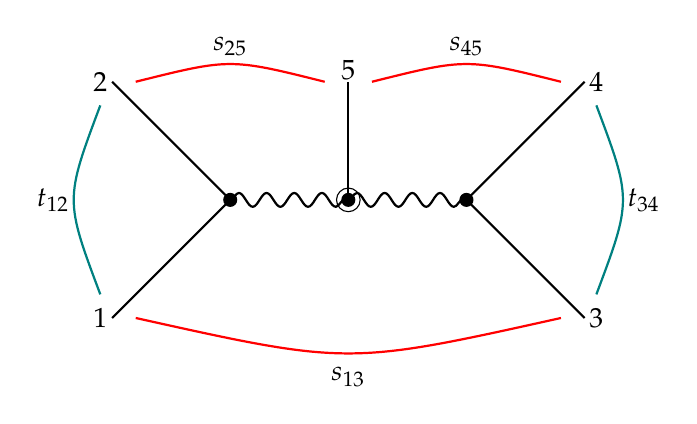
\begin{tikzpicture}[scale=1.5]
    \draw[thick] (-1,1)--(0,0);
    \draw[thick] (-1,-1)--(0,0);
    \draw[thick,snake it] (0,0)--(1,0);
    \draw[thick] (1,1) -- (1,0);
    \draw[thick,snake it] (1,0)--(2,0);
    \draw[thick] (2,0)--(3,1);
    \draw[thick] (2,0)--(3,-1);

    \draw[thick,fill] (1,0) circle (0.05cm);
    \draw[] (1,0) circle (0.1cm);
    \draw[thick,fill] (0,0) circle (0.05cm);
    \draw[thick,fill] (2,0) circle (0.05cm);
    \node at (-1.1, 1) {2};
    \node at (-1.1, -1) {1};
    \node at (3.1, 1.0) {4};
    \node at (3.1, -1.0) {3};
    \node at (1, 1.1) {5};
    % \node[fill,circle] at (1,0){};

    \draw[teal, thick] (-1.1,0.8)..controls (-1.4,0)..(-1.1,-0.8);
    \draw[teal, thick] (3.1,0.8)..controls (3.4,0)..(3.1,-0.8);
    \draw[red, thick] (-0.8,-1.0)..controls (1.,-1.4)..(2.8,-1);
    \draw[red, thick] (-0.8,1)..controls (0.,1.2)..(0.8,1.);
    \draw[red, thick] (1.2,1)..controls (2.,1.2)..(2.8,1.);

    \node at (-1.5,0) {$t_{12}$};
    \node at (3.5,0) {$t_{34}$};
    \node at (1.,-1.5) {$s_{13}$};
    \node at (0, 1.3) {$s_{25}$};
    \node at (2,1.3) {$s_{45}$};
  \end{tikzpicture}
  % \end{subfigure}
  % \includegraphics[width=0.47\linewidth]{ReggeKinScatt.pdf}
  \caption{ Regge kinematics for scattering amplitudes can be defined as $s_{13},s_{25}^2,s_{45}^2\rightarrow \frac{1}{x^2},x\rightarrow 0$ while keeping $t_{12}$ and $t_{34}$ fixed. As can be seen in Mellin space the dominant contribution to the kinematics described in figure \ref{fig:ReggeLimitVsOthers} is the same.
  % \textbf{JVB: Can we flip the image to be in accordance with Kinematics' figure?}
  }
  \label{fig:ReggeKineScatt}
\end{figure}

In this language, the exchange of operators of dimension $\Delta_1$ and $\Delta_2$ in the channels $(12)$ and $(34)$ is  respectively encoded  by the presence of poles in the Mellin amplitude
$\mathcal{M}_{5}(s_{ij},t_{ij})$ at $t_{12}=(\Delta_1-J_1+2m_1)$ and $t_{34} =  (\Delta_2-J_2+2m_2)$,
\begin{align}
  \mathcal{M}_{5}(s_{ij},t_{ij}) \approx \sum_{m_i}\frac{Q_{m_1,m_2}(s_{25},s_{45},s_{13})}{\big(t_{12}-(\tau_1+2m_1)\big)\big(t_{34}-(\tau_2+2m_2)\big)}+\dots\,,
  \label{eq:MellinamplitudepolesQ}
\end{align}
where the $\dots$ represent regular terms (or poles at other locations). Notice that the poles with $m_1=m_2=0$ are associated with the position space lightcone blocks \ref{eq:lightconeblocksspins} and $m_i>0$ correspond to corrections around the lightcone. The residue for these sequential poles is related to three-point functions involving the operators that are exchanged.


Now it remains to analyze the large $s_{ij}$ limit of the Mellin amplitude $\mathcal{M}(t_{ij},s_{ij})$.
As for the four-point case, the Casimir differential equations can be translated into Mellin space, where it transforms to a recurrence relation
that we defer to (\ref{eq:recurrencerelationsMellinCasi}) in appendix \ref{app:Blocks}.
%In particular the equation for the residue $Q_{m_1,m_2}(s_{25},s_{45},s_{13})$ is of the following form
%\begin{align}
%	\big[\mathcal{D}_{\textrm{5 pt,0}}^{(12) }+\mathcal{D}_3 \big] Q_{s_{25},s_{45},s_{13},m_1,m_2} + \mathcal{D}_2 Q_{s_{25},s_{45},s_{13},m_1-1,m_2} +\mathcal{D}_4 Q_{s_{25},s_{45},s_{13},m_1-1,m_2-1} =0
%	,
%\end{align}
%where the $(12)$ difference operators are given by expressions in \cref{app:mellinDiff}.
%The expressions for these operators are long but some of their properties are easy to state.
For the $m_i=0$ sector,  the difference equation simplifies considerably. Moreover, for each pair of spins $(J_1,J_2)$, there are $1+\textrm{min}(J_1,J_2)$ polynomial solutions which can be labeled by an integer $n$
and have the leading large $s_{ij}$ behaviour
%(\textbf{JVB: Put $\ell$ in the first position to be consistent with next equations?})
\begin{align}
  Q_{m_1,m_2}(s_{25},s_{45},s_{13}) = c_{\ell,m_1,m_2}s_{25}^{J_1-\ell} s_{45}^{J_2-\ell}s_{13}^{\ell} +\dots \,,
  \label{eq:equationleadingsijMellin}
\end{align}
where $\dots$ represent lower degree terms in the Regge limit.
Note that the $\ell$ denotes a different basis of tensor structure compared to the position space.
%  One can think of this as yet another basis. 
 We have Mellin transformed the lightcone blocks (\ref{eq:lightconeblocksspins}) and verified the behavior  (\ref{eq:equationleadingsijMellin}).
  % {\bf since we know they are not the same basis shouldn't we say it clearly?}
%This is done in the appendix \ref{}.

%The solutions are polynomials of degree $J_1$ and $J_2$ in $s_{25}$ and $s_{45}$ respectively. The difference equation, for $m_i>0$ does not increase the degree of the polynomial.
The recurrence relation (\ref{eq:recurrencerelationsMellinCasi}) can be used to derive relations between $c_{\ell,m_1,m_2}$ with different values of $m_i$
\begin{align}
   & 2 m_1 c_{\ell ,m_1,m_2} \big(d-2 (J_1+m_1+\tau _1)\big)-c_{\ell ,m_1-1,m_2} \left(\Delta _{\phi }+2 J_2-2 m_{12}-\tau _{12}-2 \ell \right)    \nonumber                       \\
   & \times\left(2 m_1+\tau _1-2 \Delta _{\phi }\right)+c_{\ell ,m_1-1,m_2-1} \left(2 m_1+\tau _1-2 \Delta _{\phi }\right) \left(2 m_2+\tau _2-2 \Delta _{\phi }\right)=0\,,
  \label{eq:RecurrencerelationMellin}
\end{align}
for the $(12)$ channel where $m_{ij}=m_i-m_j$. This particular limit is important in the Regge kinematics.
% ({\bf{need to double check}})
It gives  two recurrence relations for the coefficients $c_{\ell,m_1,m_2}$ that allow  to fix them all in terms of the seed $c_{\ell,0,0}$. As mentioned before, the label $m_i$ in the poles are related to corrections around the lightcone blocks.  Fortunately, we have worked out all these corrections for scalar operators in position space in (\ref{eq:blockscalarposallmi})  and it is a simple exercise to translate the result into Mellin space, written in (\ref{eq:ScalarblockMellin}). In particular, this solution is consistent with (\ref{eq:RecurrencerelationMellin}).

%In particular, we can check this explicit solution solves the recurrence relation above.
%\begin{figure}[h]
%\begin{centering}
%\includegraphics[scale=0.3]{ExWittDiag}
%\par\end{centering}
%\caption{Representation of an exchange Witten diagram using split representation. (picture to be improved)\label{fig:ExWittDiag}}
%\end{figure}
It is possible to construct another solution to the scalar Casimir equation, written in Mellin space, by studying conformal partial waves (or alternatively, exchanged Witten diagrams using the split representation \cite{Costa:2014kfa}). The idea behind this approach is simple, however the computation involves several steps and for this reason is given in the appendix \ref{app:ScaMellinpar}.
%Let us point out that these objects are important per se and, in fact, will play a crucial role in the conformal Regge theory for five points. 
The five-point scalar partial wave can be defined by 
% {\bf this notation of M is different from the partial wave below, which one do you prefer? Also should be the same in the next section.}
\begin{align}
  \mathcal{M}_{\nu_1, \nu_2,0,0,0}(\delta_{ij})= & {\textstyle\frac{\pi^{2h}\left[\prod_{i=1}^{2}\Gamma\left(\frac{\Delta_{2i-1}+\Delta_{2i}-t_{2i-1\,2i}}{2}\right)\left(\prod_{\sigma=\pm}\Gamma\left(\frac{h+\sigma \left(\Delta_{2i-1}-\Delta_{2i}\right)+i \nu_i}{2}\right)\right)\right]^{-1}}{\Gamma \left(\Delta _5\right) \Gamma \left(\frac{\Delta _5-i \nu _1+i \nu _2}{2}\right) \Gamma \left(\frac{t_{12}-t_{34}+\Delta _5}{2}\right) \Gamma \left(\frac{2 h-\Delta _5-i \nu _1-i \nu _2}{2}\right) \Gamma\! \left(\frac{h-t_{12}+\Delta _5-i \nu _2}{2}\right)}}\nonumber \\
                                       & {\textstyle\bigg[\Big(\prod_{\sigma=\pm}\Gamma\!\left(\frac{h-t_{12}+\sigma\Delta_5-i \nu_2}{2}\right)\Gamma\!\left(\frac{\Delta_5+\sigma i \nu_1+i \nu_2}{2}\right)\!\Big)\,\Gamma\!\left(\frac{h-t_{34}+i \nu_2}{2}\right)\Gamma\!\left(\frac{t_{12}-t_{34}+\Delta_5}{2}\right)}\nonumber                                                                                                                                                                                                                                          \\
                                       & {\textstyle\left. _3F_2\left(_{\Delta_5\,,\frac{2-h+t_{12}+\Delta_5+i\nu_2}{2}}^{\frac{t_{12}-t_{34}+\Delta_5}{2}\,,\frac{\Delta_5-i \nu_1+i \nu_2}{2},\frac{\Delta_5+i \nu_1+i \nu_2}{2}};1\right)+\Gamma\!\left(\Delta_5\right)\Gamma\!\left(\frac{t_{12}-h+\Delta_5+i \nu_2}{2}\right)\right.}\label{eq:scalarpartialMellin}                                                                                                                                                                                                      \\
                                       & {\textstyle \left(\prod_{\sigma=\pm}\prod_{i=1}^{2}\Gamma\!\left(\frac{h-t_{2i-1\,2i}+\sigma i\nu_i}{2}\right)\right)\,_3F_2\left(_{\frac{2+h-t_{12}-\Delta_5-i\nu_2}{2}\,,\frac{h-t_{12}+\Delta_5-i\nu_2}{2}}^{\frac{h-t_{12}-i\nu_1}{2}\,,\frac{h-t_{12}+i\nu_1}{2}\,,\frac{h-t_{34}-i\nu_2}{2}};1\right)\bigg]}\,,\nonumber
\end{align}
where we use the notation $\delta_{ij}=(\Delta_i+\Delta_j-t_{ij})/2$.
  %\begin{align}
  %	M(\delta_{ij})= & \frac{1}{256\prod_{i=1}^{5}\Gamma(\Delta_i+1-h)\Gamma(\Delta_\phi)\Gamma(\frac{t_{12}-t_{34}+\Delta_\phi}{2})\prod_{i=1}^{2}\Gamma(\frac{\Delta_{2i-1}+\Delta_{2i}-t_{2i-1\,2i}}{2})}                                                                                                                              \\
  %	                & \frac{\prod_{\sigma=\pm}\prod_{i=1}^{2}\Gamma\left(\frac{\Delta_{2i-1}+\Delta_{2i}+\sigma \nu_i-h}{2}\right)}{\Gamma(\frac{\Delta_\phi+h-\nu_2-t_{12}}{2})} \Gamma(\frac{\nu_2+h-t_{34}}{2})\Gamma(\frac{\Delta_\phi+\nu_{12}}{2})\Gamma(\frac{\Delta_\phi-\nu_1-\nu_2}{2})\nonumber                               \\
  %	                & {\textstyle\left[\Gamma(\frac{h+\nu_1-t_{12}}{2})\Gamma(\frac{h-\nu_1-t_{12}}{2})\Gamma(\Delta_\phi)\right.}\nonumber                                                                                                                                                                                              \\
  %	                & {\textstyle \left. \Gamma(\frac{h-\nu_2-t_{34}}{2})\Gamma(\frac{\Delta_\phi-h+\nu_2+t_{12}}{2})\,_3F_2\left(_{\frac{2+h-\nu_2-t_{12}-\Delta_\phi}{2}\,,\,\frac{h-\nu_2-t_{12}+\Delta_\phi}{2}}^{\frac{h-\nu_1-t_{12}}{2}\,,\,\frac{h+\nu_1-t_{12}}{2}\,,\, \frac{h-\nu_2-t_{34}}{2}}; 1 \right) +\right.}\nonumber \\
  %	                & {\textstyle \left. \Gamma(\frac{h-\nu_2-t_{12}-\Delta_\phi}{2})\Gamma(\frac{h-\nu_2-t_{12}+\Delta_\phi}{2})\Gamma(\frac{\Delta_\phi+\nu_1+\nu_2}{2})\Gamma(\frac{\Delta_\phi-\nu_{12}}{2})\right.}\nonumber                                                                                                        \\
  %	                & {\textstyle \left. \Gamma(\frac{\Delta_\phi+t_{12}-t_{34}}{2})\,_3F_2\left(_{\frac{2-h+\nu_2+t_{12}+\Delta_\phi}{2}\,,\,\frac{\Delta_\phi}{2}}^{\frac{\Delta_\phi-\nu_{12}}{2}\,,\,\frac{\Delta_\phi+\nu_1+\nu_2}{2}\,,\, \frac{\Delta_\phi+t_{12}-t_{34}}{2}}; 1 \right) \right]}
  %\end{align}
  % {\bf (previous text: where... anything more to add?)}
Obviously, the Mellin amplitude of the scalar conformal partial wave only depends on the variables $t_{12}$ and $t_{34}$ and it is symmetric under $\nu\rightarrow -\nu$. More importantly,  it gives a solution valid at finite $t_{ij}$ and reduces to the solution (\ref{eq:ScalarblockMellin}) when $t_{ij}$ are at the poles. This leads us to study the casimir equation away from the poles.
%.  In particular, this formula reduces to  shed some light on a solution of the Casimir equation, in the Regge limit, also for finite $t_{ij}$. 
For this purpose let us write the Mellin amplitude as
\begin{align}
  \label{eq:ReggeizePartialWaveMellinSpace}
  \mathcal{M}_{J_1,J_2}(s_{ij},t_{ij}) = s_{25}^{J_1-\ell}s_{45}^{J_2-\ell}s_{13}^{\ell}\, f(t_{12},t_{34})\,,
\end{align}
and plug it in the the recurrence relation (\ref{eq:recurrencerelationsMellinCasi}).  In turn, this leads difference equation for $t_{12}$ and $t_{34}$ that reads
\begin{align}
   & f_{00} \left(t_{12}-\tau _1\right) \left(d-t_{12}-\tau _1-2J_1\right)+f_{-20} \left(2 \Delta_\phi -t_{12}\right) \left(t_{34}-t_{12}+\Delta_\phi +2 J_2-2 \ell \right)\nonumber \\
   & +f_{-2-2} \left(2 \Delta_\phi -t_{12}\right) \left(2 \Delta_\phi -t_{34}\right)=0\,,
\end{align}
%which is obtained from (\ref{}) by taking the leading term in the limit $s_{ij}\rightarrow \infty$ with the ratio $s_{13}/( s_{25}s_{45})$ fixed and
where the subindices denote $f_{a_1a_2} \equiv f(t_{12}+a_1,t_{34}+a_{2})$. This difference equation can be further simplified by redefining $f(t_{12},t_{34})$
\begin{align}
  \tilde{f}_{00} \left(\tau_1-t_{12}\right) \left(d-2 J_1-\tau_1-t_{12}\right)+2 \tilde{f}_{-20} \left(t_{12}-t_{34}-\Delta_{\phi}-2 J_2+2 \ell \right)-4 \tilde{f}_{-2-2}=0
\end{align}
where $\tilde{f}$ is given by
\begin{align}
  \label{eq:HfunctionMellin}
  f(t_{12},t_{34}) =\frac{\tilde{f}(t_{12},t_{34})}{\Gamma(\frac{2\Delta_{\phi}-t_{12}}{2})\Gamma(\frac{2\Delta_{\phi}-t_{34}}{2})} .
\end{align}
Note that this prefactor is precisely the same as the one that comes from the Gamma functions in the definition of Mellin amplitudes (\ref{eq:scalarMellinamplitude}).
It is now simple to see that the equation for $J_1=J_2$ and generic $\ell$ can be obtained from the scalar difference equation by doing the following shifts
\begin{align}
  \Delta_{\phi}\rightarrow \Delta_{\phi}+2(J_1-\ell)	,\ \ \ \ d\rightarrow d-2J_1 .
\end{align}
This suggests that the Mellin partial wave for equal spin $J_1=J_2$ and generic $\ell$ can be obtained from (\ref{eq:scalarpartialMellin}) by doing these replacements. One way to check this statement is to build solutions with  the recursion relations in spin derived in \cite{Poland:2021xjs} (we have rederived parts of these relations in the appendix \ref{app:Blocks} using lightcone blocks) and verify that it agrees with the solution that we proposed above.% To do so we have expressed the recursion relations of \cite{Poland:2021xjs} in Mellin space and constructed solutions of the conformal partial wave from the scalar exchange. The details of this computations are relegated to appendix \ref{app:Blocks}.  {\color{blue} \bf Add appendix . This can also be used to: generate other solutions; find the change of basis between Mellin $n$ and the traditional  $\ell$. }


These solutions for Mellin amplitudes can then be inserted in (\ref{eq:ReggeMellinLimit1}) to obtain the conformal block in the Regge limit, that is
\begin{align}
   & G_{J_1,J_2,\ell,\nu_1,\nu_2}^{\circlearrowleft} (\sigma_i,\rho_i)=  \sigma_{1}^{1-J_1} \sigma_{2}^{1-J_2} \bar{\mathcal{H}}_{\nu_1\nu_2} (\xi_1,\xi_2,\xi_3)  \,,
\end{align}
with
\begin{align}
   & \bar{\mathcal{H}}_{\nu_1\nu_2} (\xi_1,\xi_2,\xi_3)=\int dt_{12}dt_{34}\, \Gamma\! \left(\frac{2\Delta_{\phi}-t_{12}}{2}\right)\Gamma\! \left(\frac{2\Delta_{\phi}-t_{34}}{2}\right)\Gamma\! \left(\frac{2 \ell -\Delta_{ \phi} +t_{12}+t_{34}-2}{2} \right)\nonumber \\
   & \qquad\qquad\qquad
  \Gamma\!\left(\frac{2 J_1-2 \ell +\Delta_{ \phi} +t_{12}-t_{34}}{2} \right) \Gamma \!\left(\frac{2 J_2-2 \ell +\Delta_{ \phi}-t_{12}+t_{34}}{2} \right)\mathcal{M}_{\nu_1,\nu_2}(t_{12},t_{34})  \nonumber                                                                         \\
   & \qquad\qquad\qquad
  \xi_1 ^{\frac{t_{34}-t_{12}-\Delta_\phi -2 J_1+2 \ell }{2} } \xi_2 ^{\frac{t_{12}-t_{34}-\Delta_\phi -2 J_2+2 \ell }{2} }\xi_3 ^{\frac{2-t_{12}-t_{34}+\Delta_\phi -2 \ell }{2}}\,,
  \label{eq:HReggeLimitMellin}
\end{align}
where $\mathcal{M}_{\nu_1,\nu_2}(t_{12},t_{34})$ is the conformal partial wave in Mellin space in the Regge limit. This expression highlights two properties of the Regge limit, firstly the limit is dominated by operators of
high spin and, secondly, it depends on three fixed cross ratios that can be thought of as angles, which is similar to  what happens in the Euclidean OPE limit as we mentioned before. In fact $\bar{\mathcal{H}}_{\nu_1\nu_2} $ solves the Casimir differential equation in the Euclidean region (\ref{eq:AngulardifferentialEquation}) but with a different eigenvalue $C$.  Let us point out that the integral (\ref{eq:HReggeLimitMellin}) can be done by picking up poles.

It follows from what was said above that  $\bar{\mathcal{H}}_{\nu_1\nu_2} (\xi_1,\xi_2,\xi_3)$ must have the same form as (\ref{eq:factorizePolynomial}), as it solves the same conformal Casimir equation.
%Equation (\ref{eq:ellDiffequation}) can be used to obtain information about the dependence in $n$ (we comment on this issue in the appendix ({\bf{\color{blue} explicit examples}})).




%%%%%%%%%%%%%%%%%%%%%%%%%%%%%%%%%%
\subsection{Comment on position space}
%%%%%%%%%%%%%%%%%%%%%%%%%%%%%%%%%%
The analysis of the Regge limit in Mellin space of the previous section exposed the similarities to flat space scattering amplitudes but it does not emphasize enough the role of analytic continuation in the cross ratios in changing the behavior of the conformal block. This aspect is clearer in  position space, in particular, in the lightcone expressions introduced in subsection \ref{sec:lightcone}. The kinematics of the Regge limit (where some pair of points are timelike while others are spacelike) can be reached from the
Euclidean configuration after doing analytic continuations in $u_2,u_4$ and $u_5$ around $0$ as explained in section \ref{sec:EucToLorent}.

The analysis is simpler for the discontinuities around  $u_4, u_5=0$ in the lightcone blocks (\ref{eq:lightconeblocksspins}) and contains most of the physics we want to highlight in this subsection. These discontinuities come from the first two terms in the denominator of (\ref{eq:lightconeblocksspins}),  provided that $u_2> 0$.
The origin of branch point at, say $u_5=0$, comes from the region $t_1 \approx 1/(1-u_5)$ where the denominator $(1-(1-u_5)t_1)$ changes sign. To deal with this it is convenient to divide the integration region in two parts, 
% {\bf JVB: I suppose the $\pi$ in the exponent of (-1) should not be there}
\begin{align}
  \int_{0}^{1} dt_1 \,\mathcal{I}\ \rightarrow \   \int_{0}^{\frac{1}{1-u_5}} dt_1 \,\mathcal{I}+(-1)^{(h_1-\tau_2-2\ell+\Delta_\phi )} \int_{\frac{1}{1-u_5}} ^{1} dt_1\,\mathcal{I}\,,
\end{align}
where the phase comes from the change of sign in the factor $(1-(1-u_5)t_1)$. The first term drops out when taking the discontinuity and so we obtain
\begin{align}
  \textrm{Disc}_{u_5=0} \int_{0}^{1} dt_1\, \mathcal{I}= \big( 1-(-1)^{(h_1-\tau_2-2\ell+\Delta_\phi )} \big) \frac{u_5}{u_5-1}\int_{0}^{1} d\tau_1 \,\mathcal{I}\,,
\end{align}
where we have changed variables to $t_1 = (u_5\tau_1 -1)/(u_5-1)$ in order to have the integration running from $0$ to $1$ again.
It is possible to repeat the same steps to take the discontinuity of $u_4$.

Recall that the cross ratios $u_4$, $u_5$ and $u_2$ approach $1$ with $\tfrac{(1-u_2)}{(1-u_4)(1-u_5)}=\tfrac{1 + \zeta}{2}$ fixed in the Regge limit.
The discontinuity in $u_4$ and $u_5$  of the lightcone block after  the Regge limit is given by
\begin{align}
  \lim_{\substack{   u_4,u_5\rightarrow 1 \\   \zeta \, \textrm{fixed}}}\textrm{Disc}_{u_5,u_4=0} \mathcal{G}
  =\frac{u_1^{\frac{1-J_1}{2}}u_3^{\frac{1-J_2}{2}  }
  (1+\zeta)^{\ell} }{\xi_2^{\Delta_2-1}\xi_1^{\Delta_1-1} 2^{\ell} }\sum_{m=0}^{\infty}
  \frac{	\dbinom{\frac{\Delta_{\phi}-\tau_1-\tau_2-2J_1-2J_2}{2}}{m}
    \left( -\frac{1+\zeta}{2} \right)^{m}
    F_1 F_2
  }{
    \Gamma\!\left(\frac{2J_1+\Delta_{\phi}-2\ell+\tau_{12}}{2}\right) \Gamma\!\left(\frac{2J_2+\Delta_{\phi}-2\ell+\tau_{21}}{2}\right)
  }\,,
  \label{eq:discInu4u5}
\end{align}
where we have used $\tau_{ij}=\tau_i-\tau_j$, the cross ratios (\ref{eq:anglesdef}) and  %({\bf \color{blue} V:change cross ratios})
\begin{align}
  %\label{eq:Fdefinition}
  F_i & =
  \frac{
    \pi
    \Gamma^2(\frac{\tau_i+2J_i}{2})\, \Gamma(\tau_i+2J_i)\,\Gamma(\tau_i+2J_i+m-1)}{
    2^{J_i-\frac{1}{2}}
    \Gamma\!\left(\frac{\tau_1+\tau_2+2J_i+2m+2\ell-\Delta_{\phi}}{2}\right)
  }
  \, \pFq{2}{1}{ \ell-J_i,\tau_{i+1}+2J_{i+1}+m-1}{\tfrac{2J_{i+1}+2m+2\ell+\tau_1+\tau_2-\Delta_{\phi}}{2}}{\frac{\zeta+1}{2} }.\nonumber
\end{align}
The discontinuities in $u_4$ and $u_5$ are enough to reveal that the discontinuities of conformal block behave with $\sigma_1^{1-J_1}\sigma_2^{1-J_2}$ in the Regge limit, which compares with $\sigma_1^{\Delta_1}\sigma_2^{\Delta_2}$ of the Euclidean block\footnote{We also need to consider the monodromy of the lightcone block around the branch point at $u_2=0$.  It is possible to do  a Mellin transform of the lightcone block and apply the method of the previous subsection to derive all discontinuities. In the appendix, we provide several checks that the discontinuity of the block in $u_2$ has the same behavior. }.
It can also be shown from the previous formula that three sequential discontinuities,  $\textrm{Disc}_{u_2,u_4,u_5}$, evaluate to zero.
Recall that four-point conformal blocks have vanishing double discontinuity.
We believe that conformal blocks have this property away from the lightcone limit.
% (\textbf{JVB: Should we conjecture some Steinman analogue for blocks?})


%%%%%%%%%%%%%%%%%%%%%%%%%%%%%%%%%%
\subsection{Conformal Regge theory for five points}
\label{subsec:SWtransform}
%%%%%%%%%%%%%%%%%%%%%%%%%%%%%%%%%%

Let us consider the representation of the five-point correlation function in terms of  conformal partial waves, and its implications for the Regge limit.
This basis  is complete and orthogonal.
Since we have more control over the analytic properties of the  partial waves in Mellin space, we consider the  expansion
\begin{align}
  \mathcal{M}(s_{ij},t_{ij} )= \sum_{J_1,J_2=0}^{\infty} \sum_{\ell=0}^{\textrm{min} \left( J_1, J_2 \right)}\int \frac{d \nu_1}{2\pi i}\,\frac{d \nu_2}{2\pi i}\, b_{J_1,J_2,\ell}(\nu_1,\nu_2)
  \mathcal{M}_{J_1,J_2,\ell}(s_{ij},t_{ij})
  \,.
  \label{eq:partialWave}
\end{align}
We suppress the dependence of the Mellin partial wave $ \mathcal{M}_{J_1,J_2,\ell} $ on the scaling dimensions, as the nontrivial analytic continuation occurs in other quantum numbers.
We have introduced  poles in the variables $ \nu_1$ and  $\nu_2 $ with residues corresponding to the OPE coefficients, using
\begin{align}
  b_{J_1,J_2,\ell}\left( \nu_1,\nu_2 \right) & \approx
  \frac{
    P_{\nu_1,\nu_2,J_1,J_2}^{\ell}
  }{
    \big( \nu_1^2- \left( \Delta_1 - h \right)^2 \big) \big( \nu_2^2- \left( \Delta_2 - h \right)^2 \big)
  }\,,
  \label{eq:residueValue}
\end{align}
where $\Delta_i=\Delta_i(J_i)$ is the dimension of the $i$-th exchanged operator of spin $J_i$.
% This is related to the conformal block expansion by a contour deformation in $ \nu_1,\nu_2 $ and using (\ref{eq:conformalpartialwave}).
We remark that  the product of the OPE coefficients   $P_{\nu_1,\nu_2,J_1,J_2}^{\ell}$ in (\ref{eq:residueValue}) is a linear combination
of those in (\ref{eq:OPE_coeffs}) that appear in the conformal block expansion. 

% {\bf JVB: Figure 12 left is wrong. In principle, there are other poles to the left of the contour coming from the sine functions (the same is true for the $\ell$ complex-plane but I think it is ok as it is). One cannot move the red contour to the left that much without encounter the pole at $\ell-1$ for instance. They are there even if for some reason they don't contribute. The easiest resolution is to center the frame close to $\ell$ similarly to what is drawn on the right or on figure 7. Btw, we should also remove one arrow from each axis.}
% {\bf Figure 12, move contour next to pole $\ell$}

\begin{figure}[t!]
  % \centering
  \begin{subfigure}[]{0.5\textwidth}
    \centering
    \resizebox{\columnwidth}{!}{
      \begin{tikzpicture}
        %name
        \draw[] (-1.2,3) -- (-1.2,2.5) -- (-2.5,2.5);
        \node[left] at (-1.2,2.8) {$J_1,J_2$};
        %axis
        \draw[-,opacity=0.3] (0,0) -- (-1.5,0);
        \draw[->,opacity=0.3,-latex'] (0,0) -- (0,3);
        \draw[-,opacity=0.3] (0,0) -- (0,-3);
        \draw[->,opacity=0.3,-latex'] (0,0) -- (5.8,0);
        %drawing points 
        % \draw[fill=black] (0,0) circle (0.05);
        % \draw[fill=black] (1,0) circle (0.05);
        \draw[fill=black] (-2,0) circle (0.05);
        \draw[fill=black] (-1,0) circle (0.05);
        \draw[fill=black] (0,0) circle (0.05);
        \draw[fill=black] (1,0) circle (0.05);
        \draw[fill=black] (2,0) circle (0.05);
        \draw[fill=black] (3,0) circle (0.05);
        \draw[fill=black] (4,0) circle (0.05);
        \draw[fill=black] (5,0) circle (0.05);
        \draw[fill=black] (0.3,1) circle (0.05);

        \draw[<-,line width=0.7,blue] (2.2,0) to[out=90,in=0] (2,0.2) to[out=180,in=90] (1.8,0) to[out=-90,in=180] (2,-0.2) to[out=0,in=-90] (2.2,0);
        \draw[<-,line width=0.7,blue] (3.2,0) to[out=90,in=0] (3,0.2) to[out=180,in=90] (2.8,0) to[out=-90,in=180] (3,-0.2) to[out=0,in=-90] (3.2,0);
        \draw[<-,line width=0.7,blue] (4.2,0) to[out=90,in=0] (4,0.2) to[out=180,in=90] (3.8,0) to[out=-90,in=180] (4,-0.2) to[out=0,in=-90] (4.2,0);
        \draw[<-,line width=0.7,blue] (5.2,0) to[out=90,in=0] (5,0.2) to[out=180,in=90] (4.8,0) to[out=-90,in=180] (5,-0.2) to[out=0,in=-90] (5.2,0);

        % \node[below] at (0.2,-0.1) {$\ell$};
        % \node[below] at (1.2,-0.1) {$\ell+1$};
        \node[below] at (2.2,-0.1) {$\ell$};
        \node[below] at (3.2,-0.1) {$\ell+1$};
        \node[below] at (4.2,-0.1) {$\ell+2$};
        \node[below] at (5.2,-0.1) {$\ell+3$};
        %main contour before deforming
        \draw[->,line width=0.7,red] (0.5,1) to[out=90,in=0] (0.3,1.2) to[out=180,in=90] (0.1,1) to[out=-90,in=180] (0.3,0.8) to[out=0,in=-90] (0.5,1);
        \draw[->,line width=0.7,red,-latex'] (-0.5,0.5) -- (-0.5,3);
        \draw[-,line width=0.7,red] (-0.5,-3) -- (-0.5,-0.5);

        \node[above right] at (0.3,1.1) {$j_i(\nu_i)$};

      \path [draw=red,thick] (-0.5, 0.5)..controls (1.8,0.5) and (1.8,-0.5)..(-0.5,-0.5) node[blue,below,xshift=+3mm]{};
      \end{tikzpicture}
    }
    % \label{fig:contourDeformationJ1J2}
  \end{subfigure}
  \hfill
  \begin{subfigure}[]{0.5\textwidth}
    \centering
    \resizebox{\columnwidth}{!}{
      \begin{tikzpicture}
        %name
        \draw[] (-1,3) -- (-1,2.5) -- (-1.5,2.5);
        \node[left] at (-1,2.8) {$\ell$};
        %axis
        \draw[-,opacity=0.3] (0,0) -- (-1.5,0);
        \draw[->,opacity=0.3,-latex'] (0,0) -- (0,3);
        \draw[-,opacity=0.3] (0,0) -- (0,-3);
        \draw[->,opacity=0.3,-latex'] (0,0) -- (5.8,0);
        %drawing points 
        \draw[fill=black] (0,0) circle (0.05);
        \draw[fill=black] (1,0) circle (0.05);
        \draw[fill=black] (2,0) circle (0.05);
        \draw[fill=black] (3,0) circle (0.05);
        \draw[fill=black] (4,0) circle (0.05);
        \draw[fill=black] (5,0) circle (0.05);
        % \draw[fill=black] (0.3,1) circle (0.05);

        % \draw[] (-0.662,0.830591) -- (-0.331,1.16178);
        % \draw[] (-0.822,0.771524) -- (-0.272,1.32161);
        % \draw[] (-0.9416,0.752275) -- (-0.252,1.44162);
        % \draw[] (-1.0434,0.751257) -- (-0.251,1.5434);
        % \draw[] (-1.133,0.761969) -- (-0.262,1.63345);
        % \draw[] (-1.215,0.78141) -- (-0.281,1.71478);
        % \draw[] (-1.289,0.807926) -- (-0.308,1.78902);
        % \draw[] (-1.357,0.84052) -- (-0.341,1.85719);
        % \draw[] (-1.420,0.878568) -- (-0.379,1.91991);
        % \draw[] (-1.478,0.921687) -- (-0.422,1.97755);
        % \draw[] (-1.530,0.96967) -- (-0.470,2.03033);
        % \draw[] (-1.578,1.02245) -- (-0.522,2.07831);
        % \draw[] (-1.621,1.08009) -- (-0.580,2.12143);
        % \draw[] (-1.659,1.14281) -- (-0.643,2.15948);
        % \draw[] (-1.692,1.21098) -- (-0.711,2.19207);
        % \draw[] (-1.719,1.28522) -- (-0.785,2.21859);
        % \draw[] (-1.738,1.36655) -- (-0.867,2.23803);
        % \draw[] (-1.749,1.4566) -- (-0.9566,2.24874);
        % \draw[] (-1.748,1.55838) -- (-1.0584,2.24772);
        % \draw[] (-1.728,1.67839) -- (-1.178,2.22848);
        % \draw[] (-1.669,1.83822) -- (-1.338,2.16941);
        %drawing circles
        \draw[<-,line width=0.7,blue] (0.2,0) to[out=90,in=0] (0,0.2) to[out=180,in=90] (-0.2,0) to[out=-90,in=180] (0,-0.2) to[out=0,in=-90] (0.2,0);
        \draw[<-,line width=0.7,blue] (1.2,0) to[out=90,in=0] (1,0.2) to[out=180,in=90] (0.8,0) to[out=-90,in=180] (1,-0.2) to[out=0,in=-90] (1.2,0);
        \draw[<-,line width=0.7,blue] (2.2,0) to[out=90,in=0] (2,0.2) to[out=180,in=90] (1.8,0) to[out=-90,in=180] (2,-0.2) to[out=0,in=-90] (2.2,0);
        \draw[<-,line width=0.7,blue] (3.2,0) to[out=90,in=0] (3,0.2) to[out=180,in=90] (2.8,0) to[out=-90,in=180] (3,-0.2) to[out=0,in=-90] (3.2,0);
        \draw[<-,line width=0.7,blue] (4.2,0) to[out=90,in=0] (4,0.2) to[out=180,in=90] (3.8,0) to[out=-90,in=180] (4,-0.2) to[out=0,in=-90] (4.2,0);
        \draw[<-,line width=0.7,blue] (5.2,0) to[out=90,in=0] (5,0.2) to[out=180,in=90] (4.8,0) to[out=-90,in=180] (5,-0.2) to[out=0,in=-90] (5.2,0);

        \node[below] at (0.2,-0.1) {$0$};
        \node[below] at (1.2,-0.1) {$1$};
        \node[below] at (2.2,-0.1) {$2$};
        \node[below] at (3.2,-0.1) {$3$};
        \node[below] at (4.2,-0.1) {$4$};
        \node[below] at (5.2,-0.1) {$5$};


        \node[left] at (-0.5,-3.0) {$\mathbf{V}=-\frac{1}{2}+i \mathbb{R}$};
        %main contour before deforming
        % \draw[->,line width=0.7,red] (0.5,1) to[out=90,in=0] (0.3,1.2) to[out=180,in=90] (0.1,1) to[out=-90,in=180] (0.3,0.8) to[out=0,in=-90] (0.5,1);
        \draw[->,line width=0.7,red,-latex'] (-0.5,-3) -- (-0.5,3);

        % \node[above right] at (0.3,1.1) {$j(\nu)$};

      \end{tikzpicture}
    }
  \end{subfigure}
  \caption{Integration contours for the spin quantum numbers $J_1,J_2$,  as well as $ \ell$.
    The blue contour is the Euclidean contour, whereas the red contour is the Regge contour.
    We assume the leading Regge pole in the $J_i$-plane is located at $j_i(\nu)$ and that there are no
    dynamical poles in the $\ell$ plane. 
    Red contour is understood to be deformed to the right of the other infinite series of poles depending on $ \ell $ lying on the left in the $J_i$-plane.
  }
  \label{fig:contourDeformationJ1J2}
\end{figure}

We would like to provide a Sommerfeld-Watson representation of (\ref{eq:partialWave}).
First, we swap the range of summations as
\begin{align}
  \mathcal{M}(s_{ij},t_{ij} )
  = \sum_{\ell=0}^{ \infty}
  \sum_{J_1,J_2=\ell}^{\infty}
  \int \frac{d \nu_1}{2\pi i}\,\frac{d \nu_2}{2\pi i}\, b_{J_1,J_2,\ell}(\nu_1,\nu_2)
  \mathcal{M}_{J_1,J_2,\ell}(s_{ij},t_{ij})
  \,.
  \label{eq:partialWaveSwapped}
\end{align}
% Then, we analytically continue in $ \ell $ before dealing with the spins $ J_1,J_2 $.
% It is difficult to visualize all the contours in the complex $ J_1,J_2,\ell $ plane, as they form a three dimensional subspace of  a six real dimensional space.
% We represent in terms of individual complexified variables $ J_1, J_2, \ell $, as shown in figure \ref{fig:contourDeformationJ1J2}.
%Multiple figures 
Next, we   analytically continue in the spin quantum numbers.
However, the $ b_{J_1,J_2,\ell} $ are not expected to have a unique
analytic  continuation in   the quantum numbers. For that reason we need to consider
their    \textit{signatured} counterparts.

Let us remind the reader the analogous construction \cite{Costa:2012cb} for the four-point correlator $ \mathcal{A}( u,v ) $ in terms of the cross ratios
\begin{align}
  u =  \frac{x_{12}^2 x_{34}^2 }{x_{14}^2 x_{23}^2 } \,, \qquad v = \frac{x_{13}^2 x_{24}^2 }{x_{14}^2 x_{23}^2}\,.
\end{align}
% The function $ \mathcal{A}(u,v) $ has nontrivial monodromies in the complex $ v $ plane around $ v = 1 $ and $ v= \infty $.
% % Consider a swap of $ x_3 \leftrightarrow x_4 $, which maps $ v $ to $ 1/u$ and $ u $ to $ u/v $.
% In this case, we split the amplitude in terms of \textit{signatured} amplitudes \footnote{Consider $ \mathcal{A}(z) = \log z $ as a toy model. It has a branch point at $ z=0 $ with monodromy $ 2\pi i $. However, $ \log (1/z) $ also has branch point at $ z=0 $ but with monodromy $ -2\pi i $. Therefore, one can define $ \mathcal{A}_{+} = \log z  + \log (1/z)$ which has trivial monodromy around $ z=0 $.  }, $\mathcal{A}_{\theta = \pm}$, such that $ \mathcal{A} (u,v) = \mathcal{A}_{+} + \mathcal{A}_{-} $.
% These are related by the following relation
% \begin{align}
% 	\mathcal{A}_{\theta}( u,v ) =
% 	\frac{1}{2}
% 	\left[
% 		\mathcal{A}( u,v )
% 		+ \theta
% 		\mathcal{A}\!\left( \frac{u}{v},\frac{1}{v}\right)
% 		\right] .
% 	\label{eq:signaturedAmpFourPoints}
% \end{align}
% They are designed to have cuts in the complex $ v $ plane such that $ \mathcal{A}_{+} $ has a nontrivial discontinuity in $ t $ channel, i.e., around $ v = 1 $, and $ \mathcal{A}_{-} $ has a nontrivial discontinuity in $ u $ channel, i.e., around $ v = \infty $.
After expanding in Euclidean partial waves, we can write the correlation function as
\begin{align}
  \mathcal{A}( u,v)
  =
  \displaystyle\sum_{J=0}^{\infty}
  \displaystyle\int_{\frac{d}{2}+i \mathbb{R}}
  \frac{d\Delta}{2\pi i}\,
  c_{\Delta,J}\,
  F_{\Delta,J} ( u,v )
  \,,
  \label{eq:EuclideanInversion}
\end{align}
where $ c_{\Delta,J} $ denotes the OPE function and $ F_{\Delta,J} $ is the Euclidean partial wave.
It can be transformed to Mellin space as
\begin{align}
  \mathcal{M}(s,t)
  =
  % \frac{1}{2\pi i}
  \displaystyle\sum_{J=0}^{\infty}
  \int_{\frac{d}{2}+i \mathbb{R}}
  \frac{d\Delta}{2\pi i}\,
  c_{\Delta,J}\,
  \mathcal{M}_{\Delta,J} (s,t)
  \,.
  \label{eq:MellinInversion}
\end{align}
% The signatured partial wave is defined according to \cref{eq:signaturedAmpFourPoints}, whereas the signatured OPE function is the component of the signatured correlator on the partial wave.
Again, the OPE function $ c_{\Delta,J} $ is not uniquely defined in the complex $ J $ plane.
Thus, we define the signatured OPE function $ c_{\Delta,J}^{\theta} $ by
\begin{align}
  \mathcal{M}_{\theta} (s,t)
  =
  \displaystyle\sum_{J=0}^{\infty}
  \displaystyle\int_{\frac{d}{2}+i \mathbb{R}}
  \frac{d\Delta}{2\pi i}\,
  c_{\Delta,J}^{\theta}\,
  \mathcal{M}_{\Delta,J}^{\theta} (s,t)
  \,,
  \label{eq:signaturedMellin}
\end{align}
where the signatured Mellin partial waves are given by
\begin{align}
  \mathcal{M}_{\Delta,J}^{\theta} (s,t)
  =
  \frac{1}{2}
  \big[
    \mathcal{M}_{\Delta,J} (s,t)
    + \theta
    \mathcal{M}_{\Delta,J}(-s,t)
    \big]
  \,,
  \label{eq:signaturedMellinAmp4pt}
\end{align}
with $\theta=\pm$.
The signatured Mellin amplitude allows for a unique analytic continuation of the
signatured OPE function $ c_{\Delta,J}^{\theta} $ \cite{Caron-Huot:2017vep}.
The problem of the non-signatured OPE function can be traced back  the factor of $(-1)^J$ that appears
in the transformation $s\to-s$,
%$\mathcal{M}_{\Delta,J}(-s,t) = (-1)^J  \mathcal{M}_{\Delta,J}(s,t)$
which follows
%  can be hinted 
from the large $s$
behaviour $\mathcal{M}_{\Delta,J}(s,t) \approx s^J$.

A similar construction can be done for five-point functions.
We split the full correlator into eight parts depending on the \emph{signature} denoted by $ \mathbb{\theta} = (\theta_1,\theta_2,\theta_{12}) $ where each component can be $\pm$.
% They are dual to the quantum numbers $ J_1,J_2,\ell $, respectively.
We define the  \textit{signatured} amplitudes as
\begin{align}
   & \mathcal{M}_{\theta}(s_{25},s_{45},s_{13})
  %  \nonumber \\ 
  %  & 
  =
  \frac{1}{8}
  \big[
    \mathcal{M}(s_{25},s_{45},s_{13})
    +
    \theta_1
    \mathcal{M}(-s_{25},s_{45},s_{13})
    +
    \theta_{2}
    \mathcal{M}(s_{25},-s_{45},s_{13})
  \nonumber                                     \\
   &
    +
    \theta_1 \theta_{2}
    \mathcal{M}(-s_{25},-s_{45},s_{13})
    +
    \theta_{12}
    \mathcal{M}(-s_{25},-s_{45},-s_{13})
    +
    \theta_1 \theta_{12}
    \mathcal{M}(s_{25},-s_{45},-s_{13})
    \nonumber
  \\
   &
    +
    \theta_{12} \theta_{2}
    \mathcal{M}(-s_{25},s_{45},-s_{13})
    +
    \theta_1 \theta_{12} \theta_{2}
    \mathcal{M}(s_{25},s_{45},-s_{13})
    \big]
  \,.
  \label{eq:signaturedMellinAmp}
\end{align}
This equation is suitable only for $s_{ij} \gg 1$.
We also suppress the dependence on $ t_{ij} $ for brevity.
We justify it by using the properties of the Mellin partial wave (\ref{eq:ReggeizePartialWaveMellinSpace})  which,
in terms of $ J_i'=J_i-\ell $,  behaves in the  Regge limit as
\begin{align}
  \mathcal{M}_{J_1',J_2',\ell}(s_{ij},t_{ij}) & = s_{25}^{J_1'}s_{45}^{J_2'} \, s_{13}^{\ell}\, f(t_{12},t_{34})\,.
  % \mathcal{M}^{\theta}_{J_1,J_2,\ell} &= s_{25}^{J_1'} s_{45}^{J_2'} s_{13}^{\ell_\phantom{1}}
\end{align}
By analogy with the four-point case, we expect that OPE functions associated with the expansion of the signatured amplitudes in
(\ref{eq:signaturedMellinAmp}) have a unique analytic continuation in all quantum numbers $J_1',J_2',\ell$.
It would be interesting to put this on a firm footing by deriving dispersion relations along the lines of \cite{Caron-Huot:2017vep}.
The full Mellin amplitude can then be written in terms of the signatured Mellin amplitude as
\begin{align}
  \label{eq:fullMellinFromSignature}
  \mathcal{M}(s_{25},s_{45},s_{13} ) & = \sum_{\theta \in \{ -1,1 \}^{3}} \mathcal{M}_{\theta} (s_{25},s_{45},s_{13} )
  \,.
\end{align}

% We would like to perform the integral over the $ \ell $ contour by splitting the odd and even values.
% This is analogous to the case of five point S matrix, wherein the quantum number $ m $ was split into positive and negative values.
% Defining $ J_i' = J_i-\ell $ and signatured partial wave as $ \mathcal{M}_{J_1',J_2',\ell}^{\theta}(u_i) $, we write
In terms of the signatured analogue of partial waves defined through (\ref{eq:signaturedMellinAmp}), we write
\begin{align}
  \mathcal{M}_{\theta} ( s_{ij},t_{ij} )=
  \sum_{\ell=0}^{\infty} \sum_{J_1',J_2'=0}^{\infty}
  \int \frac{d \nu_1}{2\pi i}\,
  \frac{d \nu_2}{2\pi i}\, b_{J_1',J_2',\ell}^{\theta}(\nu_1,\nu_2) \mathcal{M}_{J_1',J_2',\ell}^{\theta}(s_{ij}, t_{ij})
  \,.
  \label{eq:partialWaveSwappedOddEven}
\end{align}
Next we  perform a Sommerfeld-Watson transform on the $ \ell $ contour.
% Since we have more control over the analytic properties of the Euclidean partial waves, we perform these calculations in Mellin space.
% As discussed before, in the Regge limit the Mellin amplitude of the partial wave is given by (\ref{eq:ReggeizePartialWaveMellinSpace}).
% Note that the leading power of the polynomial depends only on $ J_1'$ and $J_2' $.
% Thus, the Mellin amplitude of the signatured correlator $ \mathcal{A}_{\theta} $ denoted by $ \mathcal{M}_{\theta} ( s_{ij},t_{ij}) $, is given by
% Signatured Mellin amplitudes are defined as
% \begin{align}
% 	\label{eq:signaturedMellinAmp}
% 	 & \mathcal{M}_{\theta}(s_{25},s_{45},s_{13})
% 	%  \nonumber \\ 
% 	%  & 
% 	=
% 	\frac{1}{8} 
% 	\big[
% 		\mathcal{M}(s_{25},s_{45},s_{13})
% 		+
% 		\theta_1
% 		\mathcal{M}(-s_{25},s_{45},s_{13})
% 		+
% 		\theta_{2}
% 		\mathcal{M}(s_{25},-s_{45},s_{13})
% 	\nonumber                                     \\
% 	 &
% 		+
% 		\theta_1 \theta_{2}
% 		\mathcal{M}(-s_{25},-s_{45},s_{13})
% 		+
% 		\theta_{12}
% 		\mathcal{M}(-s_{25},-s_{45},-s_{13})
% 		+
% 		\theta_1 \theta_{12}
% 		\mathcal{M}(s_{25},-s_{45},-s_{13})
% 		\nonumber
% 	\\
% 	 &
% 		+
% 		\theta_{12} \theta_{2}
% 		\mathcal{M}(-s_{25},s_{45},-s_{13})
% 		+
% 		\theta_1 \theta_{12} \theta_{2}
% 		\mathcal{M}(s_{25},s_{45},-s_{13})
% 		\big]
% 	\,.
% \end{align}
% This equation is suitable only for high energies as we are using $ u_{ij} \approx -s_{ij} $ upto finite terms.
% We have also suppressed the dependence on $ t_{ij} $ for brevity.
% 
% We provide a heuristic justification for the above definition. 
% 
% First, we note that each of the variables $ s_{25},s_{45},s_{13} $ has a series of poles on the real axis on both right half plane and left half plane, as can be seen from (\ref{eq:MellinAmpDefinition}).
% We choose a definition for a signature triplet $ \theta $ and corrrespond it to the series of poles on the real axis, positive or negative depending on the $ \theta_i=1 $ or $ -1 $.
% For instance, $ \theta=(1,1,1) $ corresponds to the series of poles on the positive real axis in each of $ s_{13}, s_{25}, s_{45} $.
% Then, we require that the other series of poles have zero residue.
% It uniquely fixes the signatured Mellin amplitude \cref{eq:signaturedMellinAmp}, upto an arbitrary constant which we choose to be $ 1/8 $, such that,
% The full Mellin amplitude can be written in terms of the signatured Mellin amplitude as
% \begin{align}
% 	\mathcal{M}(s_{25},s_{45},s_{13} ) & = \sum_{\theta \in \{ -1,1 \}^{3}} \mathcal{M}_{\theta} (s_{25},s_{45},s_{13} )
% 	\,.
% \end{align}
First, we replace the summation over $ \ell $ by an integral over the blue contour shown in figure \ref{fig:contourDeformationJ1J2}.
Then we  move the contour around the non-negative integers to a vertical contour $ \mathbf{V} $ located at $ -1/2+i \mathbb{R} $, as shown in figure \ref{fig:contourDeformationJ1J2}.
We assume that we do not encounter any poles during this procedure.
This assumption is inspired by an analogous procedure for the five particle S-matrix.
Indeed the quantum number $ \ell $ labels a choice of tensor basis for three-point functions and therefore should not
have a dynamic content, just like the
helicity quantum number for the S-matrix  \cite{Abarbanel:1972ayr}.
Thus after deforming the $\ell$ contour we have
\begin{align}
  \mathcal{M}_{\theta} ( s_{ij},t_{ij}) & =
  \int_{\mathbf{V}} \frac{d \ell}{2\pi i} \frac{1}{\sin ( \pi \ell)}
  \sum_{J_1',J_2'=0}^{\infty}
  \int \frac{d \nu_1}{2\pi i}\,
  \frac{d \nu_2}{2\pi i}\, b_{J_1',J_2',\ell}^{\theta}(\nu_1,\nu_2)\mathcal{M}_{J_1',J_2',\ell}^{\theta}(s_{ij},t_{ij})
  \,.
\end{align}

Next we analytically continue in $ J_1'$ and $J_2' $.
The analytic structure in these variables is analogous to the case of four-point correlation functions.
Figure \ref{fig:contourDeformationJ1J2} shows the analytic structure of the integrand in (\ref{eq:partialWaveSwappedOddEven}).
In particular there is a leading Regge pole in the $ J_i $ plane at $ J_i =j_i( \nu_i ) $ given by
\begin{align}
  \left[ \Delta_i\big(j_i( \nu_i )\big)- h \right]^{2}  -\nu_i^{2}  = 0\,.
\end{align}
% The leading behaviour of the function $ \mathcal{M} $ is derived in (\ref{eq:ReggeizePartialWaveMellinSpace}), namely
% \begin{align}
% 	\label{eq:ReggeizePartialWaveMellinSpaceRepeat}
% 	\mathcal{M}_{J_1,J_2,\ell}(s_{ij},t_{ij})&= s_{25}^{J_1}s_{45}^{J_2} \, \eta^{\ell}\, f(t_{12},t_{34})\,.
% \end{align}
% We remind the reader that $ \eta = s_{13}/(s_{25} s_{45}) $ and $ f $ is defined in (\ref{eq:HfunctionMellin}).
Picking the poles in the complex spin planes at $J_1'= j_1(\nu_1)-\ell$ and $J_2'= j_2(\nu_2)-\ell$,  we obtain
the following expression for the signatured correlators
\begin{align}
  \mathcal{M}_{\theta}
  =
  \int
  \frac{d \nu_1}{2\pi i}\,
  \frac{d \nu_2}{2\pi i}
  \, s_{25}^{j_1( \nu_1)} s_{45}^{j_2( \nu_2)}
  \int_{\mathbf{V}} \frac{d \ell}{2\pi i}\,
  \,
  \frac{
    b_{j_1(\nu_1),j_2(\nu_2),\ell}^{\theta}(\nu_1,\nu_2) \,
    f_{\nu_1,\nu_2,\ell}^{\theta}(t_{ij})\, \eta^{\ell}
  }{\sin(\pi \ell) \sin\!\big(\pi (j_1(\nu_1)-\ell)\big) \sin\!\big(\pi (j_2(\nu_2)-\ell)   \big)}
  \,,\label{eq:pickingJ1J2poles}
\end{align}
where $ f_{\nu_1,\nu_2,\ell}^{\theta} $ is defined as the signatured analogue of $ f $ in (\ref{eq:HfunctionMellin}).
Thus, in the Regge limit the full correlator has the form
\begin{align}
  \mathcal{M}
  =
  \int
  \frac{d \nu_1}{2\pi i}\,
  \frac{d \nu_2}{2\pi i}
  \, s_{25}^{j_1\left( \nu_1 \right)} s_{45}^{j_2\left( \nu_2 \right)}
  \int_{\mathbf{V}} \frac{d \ell}{2\pi i}\, \eta^{\ell}  g_{\nu_1,\nu_2,\ell}(t_{ij})
  \,,\label{eq:final}
\end{align}
where the function $g_{\nu_1,\nu_2,\ell} (t_{ij})$ is defined from replacing (\ref{eq:pickingJ1J2poles}) in (\ref{eq:fullMellinFromSignature}).
This allows us to represent the Reggeized Mellin amplitude in terms of the operator content of the leading Regge trajectories and their couplings to the external states.

%As for the four point function  \cite{Costa:2017twz}, we expect that the $\nu$ integrals can be done by saddle point, leading to the behavior $\mathcal{M} \sim s_{25}^{j_1^*} s_{45}^{j_2^*} F(t_{ij})$, where $j_i^*$

\section{Conclusions}
\label{sec:conclusions}

We have discussed the generalization of the Regge limit to higher-point correlation functions in conformal field theories in general dimensions.
For the case of five-point functions, we defined the five-variable generalization of the Mack polynomials, and discussed its properties.
Using the leading order behavior of these polynomials, we studied the multi-Regge limit of the correlator which is dominated by the leading Regge trajectories.
% We also argued that there are no additional singularities in the complexified quantum numbers apart from the poles associated with the complexified spin.

By considering the implications of multi-Regge limit in Mellin space, we arrived at a proposal for the kinematics of the multi-Regge limit in  position space.
We studied the behavior of the conformal block in this limit, using the recent results on lightcone blocks for higher-point functions.
To compute the monodromies of the conformal block, we also used some techniques from the study of hypergeometric functions. 

Mellin space is a good place to study the multi-Regge limit of the correlators.
We expect that the multi-Regge limit for conformal field theories in Mellin space is analogous to that of the flat space S matrix in Mandelstam space.
The generalization of the partial wave expansion in the S matrix is done in \cite{White:1976qm}, for four dimensional quantum field theories.
Analogous generalization of the partial wave expansion is within reach for three dimensional CFTs for $n$-point functions.
We would benefit from the fact that there are no representations of the rotation subgroup of the conformal group in three dimensions with more than one rows in the Young's tableaux.
However, for higher dimensions, there will be proliferation of indices labelling the internal vertices.


In the process, we also discussed a novel basis of three-point functions of operators with spin $\left(  J_1,J_2,0  \right)$, respectively.
This basis is useful for study of Euclidean OPE limit as it leads to the analytic expression for the conformal block in this limit.
These expressions appear to be a natural generalization of the Wigner $ d $ function used in the S matrix.
This suggests that the basis used in the literature for three-point functions of operators with spin $\left(  J_1,J_2,J_3  \right)$ might not be the most natural one for the study of Euclidean conformal blocks.
Given the importance of conformal blocks in numerical bootstrap, it would be interesting to study the properties of this basis in more detail.
The case of $\left(  J_1,J_2,J_3  \right)$ three-point function is accessible in the Euclidean OPE limit of six-point function in the snowflake channel.

The new basis appears to be useful to arrive at a Euclidean inversion formula for the five-point functions, mainly due to simple orthogonality properties.
While the study of analytic structure of the correlator of higher-point functions is still in its infancy, we expect that it admits a drastic simplification in the multi-Regge limit.
It would be interesting to derive an inversion formula and dispersion relation in the multi-Regge limit for CFTs, along the lines of \cite{NotesOnMultiRegge}.
An important ingredient is the multivariable generalization of the Cauchy formula, called the Bargman-Weil formula.

Finally, in the S matrix case, a crucial ingredient for the absence of singularities in $ \ell $ was the use of Steinmann relations.
% We have assumed that the Steinmann relations hold for the CFTs.
It would be interesting to explore the analogue of Steinmann relations in CFTs.
%Since these relations follow from basic properties of any quantum field theory, it is likely that they hold for CFTs as well. In particular, they might further constrain  holographic supergravity amplitudes for more than four point functions. See \cite{Caron-Huot:2016owq} for analogous progress in the weakly coupled $ \mathcal{N}=4 $ super Yang-Mills.

%\input{Folder/Filename}

\begin{appendices}
  \input{Appendices/appendix2.tex}
  % 	% \input{Folder/Filename}
\end{appendices}

% \configbibliography[]{Bibliography}
% \begin{appendices}
% 	\input{Appendices/AppendixB}
% 	% \input{Folder/Filename}
% \end{appendices}
% \part{Conclusions}
% Chapter Template

\chapter{Conclusions} % Main chapter title
\label{part:conclusions}

In this thesis, we have discussed two aspects of conformal Regge theory.

In the second chapter, we considered the generalization of the Optical theorem to $ AdS $.
This allowed us to write a formula that relates one loop CFT data in terms of tree level CFT data.

It would be interesting to use this formula to constrain CFT data at one loop in $ AdS $ in various supergravity approximations.
More generally, there are various techniques in the scattering amplitude literature which deal with Feynman diagrams at higher loops which deal with only on-shell data.
It would interesting if they have an analogous construction in $ AdS $.
Since unitarity plays an important role in those constraints, we expect our formula to be useful in that context.

It would be interesting if this formula can be generalized to higher loops.
We commented about it in the conclusion of the second chapter.
It is known that in the supergravity approximation, the loop diagrams can be resummed in the Regge limit.
It would be interesting to generalize it beyond the supergravity approximation.
Recently, there has been a lot of progress in the correlation functions on the boundary of $ AdS_3 $ in terms of Wess-Zumino-Witten models \cite{Eberhardt:2021vsx}.
With or without supersymmetry, these models provide a good arena to test such a resummation procedure in $ AdS $.
It would provide a model of eikonal resummation at finite `t Hooft coupling which can be interpolated between weak and strong coupling.

In particular, cutting rules in flat space suggest that one can always decompose higher loop Feynman diagrams in terms of lower loop diagrams.
Analogously, Witten diagrams might follow such a recursion.

In the third chapter, we considered the generalization of the Regge theory to higher point correlation functions.
As the study of higher point correlation functions is in a nascent stage, there are several avenues of interest.

We have provided a novel basis for three point functions of spinning operators.
This is necesary to establish the orthogonality of the conformal partial waves.
It would be interesting to explicitly write this orthogonality relation and the corresponding Euclidean inversion formula.
Then, one can use the prescription for the Regge limit proposed in the third chapter along with boundedness assumption to arrive at an inversion formula.
This would establish rigidity that is much stronger than the the one imposed by analyticity in spin.

More generally, the study of the causality constraints of the correlation functions has been done only in the four point case.
It would be interesting to generalize this to higher point cases.
Steinmann relations are known to be powerful in the weakly coupled maximally supersymmetric Yang-Mills theory in four dimension (SYM).
It would be interesting to work out their implications in the strongly coupled limit.

Finally, the topic of Regge theory is chiefly inspired by the experimental data.
It would be interesting if the lessons learnt from the higher supersymmetric examples teach us something about the Regge trajectories of the Quantum chromodynamics.
After all, super Yang-Mills theory is a close cousin of the Quantum chromodynamics with a different matter content.
Is there a way to deform the leading Regge trajectory to predict the correspoding leading Regge trajectory of Quantum chromodynamics?
Hopefully, a more detailed understanding of the leading trajectory of conformal Regge theory and SYM will teach some lessons.



\cleardoublepage


% Another approach to appendices, all appendices as chapters the final thesis part
%%% APPENDICES %%%
%\appendixpage
% \input{Folder/Filename}


%-----------------------------------------------------------------------------------
%	BIBLIOGRAPHY
%-----------------------------------------------------------------------------------

\backmatter % End front matter

% \addvspacetoc{5mm} % Add a gap in the Contents, for aesthetics

% \configbibliography[chapter|part]{<name of bib header>} 

%\nocite{*}
\bibliographystyle{unsrt}
%\bibliographystyle{apsrev4-1-etal} % Use the utphys, apsrev4-1, kp and more BibTeX style for formatting the Bibliography
\bibliography{Bibliography}
% The references are stored in the file "Bibliography.bib"


\end{document}
